%% Master's Thesis: Network Effects of Social Media Use on Well-Being
%% University of Oslo - Department of Mathematics
%% This is the master document.
%% Individual chapters are in the chapters/ folder.

%% Add UiO templates folder to LaTeX search path
\makeatletter
\def\input@path{{uio-templates/}}
\makeatother

\documentclass[UKenglish]{uiomasterthesis}

%% Load preamble (packages, commands, settings)
%% Preamble: Packages, Settings, and Custom Commands

%% Encoding and Language
\usepackage[utf8]{inputenc}
\usepackage[T1]{fontenc}
\usepackage{babel}
\usepackage{textcomp}
\usepackage{url}
\urlstyle{sf}

%% UiO Packages
\usepackage{uiomasterfp}    % Front page

%% Mathematics
\usepackage{amsmath, amssymb, amsthm}
\usepackage{mathtools}      % Extensions to amsmath
\usepackage{bm}             % Bold math symbols (\bm{})
\usepackage{dsfont}         % Double-stroke font (\mathds{1} for indicator)

%% Tables and Figures
\usepackage{booktabs}       % Professional tables (\toprule, \midrule, \bottomrule)
\usepackage{graphicx}       % Include graphics
\usepackage{float}          % Better float placement [H]
\usepackage{array}          % Extended column types

% Path to figures and UiO templates
\graphicspath{{figures/}{uio-templates/}}

%% Algorithms
\usepackage{xcolor}         % Colours (needed by hyperref)
\usepackage{algorithm}
\usepackage{algpseudocode}

%% Bibliography
\usepackage{csquotes}       % Recommended by biblatex for smart quote handling
\usepackage[
    style=authoryear,
    backend=biber,
    maxcitenames=2,
    maxbibnames=99,
    uniquename=false,
    uniquelist=false
]{biblatex}
\addbibresource{references.bib}

%% Add comma between author and year in citations
\renewcommand*{\nameyeardelim}{\addcomma\space}

%% Cross-References and Hyperlinks
\usepackage{hyperref}
\hypersetup{
    colorlinks=true,
    linkcolor=blue!70!black,
    citecolor=green!50!black,
    urlcolor=blue!70!black,
    pdfauthor={Aslak Hellevik},
    pdftitle={Network Effects of Social Media Use on Well-Being}
}

\usepackage[nameinlink, capitalise, noabbrev]{cleveref}

%% Theorem Environments
\theoremstyle{plain}
\newtheorem{theorem}{Theorem}[chapter]
\newtheorem{proposition}[theorem]{Proposition}
\newtheorem{lemma}[theorem]{Lemma}
\newtheorem{corollary}[theorem]{Corollary}

\theoremstyle{definition}
\newtheorem{definition}[theorem]{Definition}
\newtheorem{assumption}{Assumption}[chapter]
\newtheorem{example}[theorem]{Example}

\theoremstyle{remark}
\newtheorem{remark}[theorem]{Remark}

%% Cleveref names for assumptions
\crefname{assumption}{Assumption}{Assumptions}
\Crefname{assumption}{Assumption}{Assumptions}

%% Custom Commands: Vectors and Matrices
\newcommand{\vect}[1]{\bm{#1}}              % Vectors: bold italic
\newcommand{\mat}[1]{\mathbf{#1}}           % Matrices: bold upright
\renewcommand{\vec}[1]{\vect{#1}}           % Override default \vec

%% Custom Commands: Probability and Statistics
\newcommand{\E}{\mathbb{E}}                 % Expectation
\newcommand{\Var}{\operatorname{Var}}       % Variance
\newcommand{\Cov}{\operatorname{Cov}}       % Covariance
\newcommand{\N}{\mathcal{N}}                % Normal distribution
\newcommand{\iid}{\stackrel{\text{iid}}{\sim}}  % iid symbol

\newcommand{\pto}{\xrightarrow{p}}          % Convergence in probability
\newcommand{\dto}{\xrightarrow{d}}          % Convergence in distribution

%% Custom Commands: Linear Algebra
\newcommand{\tr}{\operatorname{tr}}         % Trace
\newcommand{\rank}{\operatorname{rank}}     % Rank
\newcommand{\diag}{\operatorname{diag}}     % Diagonal

%% Custom Commands: Number Sets
\newcommand{\RR}{\mathbb{R}}                % Real numbers

%% Custom Commands: Model-Specific Notation
% SMU averages
\newcommand{\sbar}{\bar{s}}                 % Average SMU of peers
\newcommand{\ybar}{\bar{y}}                 % Average WB of peers

% Key matrices
\newcommand{\Ay}{\mat{A}_y}                 % I - gamma_3 G
\newcommand{\As}{\mat{A}_s}                 % I - beta_1 G

% Parameter vectors
\newcommand{\thetavec}{\bm{\theta}}         % Generic parameter vector
\newcommand{\gammavec}{\bm{\gamma}}         % Gamma parameters

% Indicator function
\newcommand{\one}{\mathds{1}}               % Indicator function

%% Miscellaneous Settings
% Prevent widows and orphans
\widowpenalty=10000
\clubpenalty=10000

% Better spacing in equations
\allowdisplaybreaks

% Equation numbering by chapter
\numberwithin{equation}{chapter}



%% Document Metadata
\title{Network Effects of Social Media Use on Well-Being}
\subtitle{From Agent-Based Models to Statistical Inference}
\author{Aslak Hellevik}

%% Begin Document
\begin{document}

%% Front Page (UiO official format)
\uiomasterfp[
    program={SMR: Statistics},
    long,                           
    supervisors={Tobias Dahl \& Ingrid Hobæk Haff},
    colour=green,
    date={Spring 2026}
]

%% Front Matter
\frontmatter

% Abstract

%% Abstract

\begin{abstract}

Most empirical research on the relationship between social media use (SMU) and well-being (WB) does not model network effects on individual outcomes. This thesis shows that this omission can bias causal estimates and develops statistical methods for network-aware inference to address this gap. The thesis is methodological, and the methods are not applied to real data.

Agent-based models are applied as a bottom-up approach to simulate networked agent behaviour. Cross-sectional ordinary least squares, panel fixed effects, and randomised controlled trials are all shown to produce biased estimates when applied to data with underlying networked dynamics. This motivates explicit network modelling.

We develop the recursive CoMO model, a cross-sectional structural model with network effects, and formalise the \emph{cost of missing out} (CoMO) concept introduced in the SMU--WB context by \textcite{DahlFoldnesGronneberg2024} as a novel non-linear term capturing asymmetric peer comparison. This model lets an individual's WB depend both on their own SMU and on the \emph{relative} difference between their own and their peers' SMU\@. We derive maximum likelihood estimators and analytical Hessian matrices for the SMU and WB equations, and a two-stage least squares estimator for the latter. Monte Carlo simulations provide evidence of low bias and near-nominal confidence interval coverage.

The model is extended to the simultaneous CoMO model with feedback from WB to SMU\@. Using Banach's fixed-point theorem, we prove existence and uniqueness of the equilibrium under a contraction condition, and derive a full information maximum likelihood estimator. The estimator's properties are validated in an initial Monte Carlo simulation.

\end{abstract}


% Acknowledgements
%% Acknowledgements
\begin{preface}

The starting point for this thesis was my multidisciplinary interest, which made me want to apply statistical rigour to a real-world problem. This is the result of that attempt.

I began the thesis work by using simulations to explore and visualise intricacies of the problem of estimating the causal effect of social media use on well-being. After the first two months, I realised the need for more statistical rigour, and made a major change of direction. This led me to the topic for the main body of the thesis: developing statistical inference for network models.

The result is a bidirectional story. Complex simulations apply a bottom-up approach, showing the difficulties of the problem. Top-down, statistically rigorous models point towards a resolution, but do not yet have the sophistication required for a full answer. I have enjoyed working with the problem in this way, and hope that my contribution provides a step towards closing the gap in the future.

I want to thank Tobias Dahl for his energy, optimism, and encouragement throughout the process. I would also like to thank my internal supervisor Ingrid Hobæk Haff for help with the formal requirements of the programme. Special thanks go to Steffen Grønneberg for tremendous support during the most uncertain time of the work, and for helping me find the way forward.

Finally, I want to thank my family and friends for all the interest they have shown in this project, and for their feedback on drafts.

\vspace{3cm}
\noindent Oslo, May 2026

\vspace{1cm}
\noindent Aslak Hellevik

\end{preface}


% Declaration of AI usage
%% Declaration of AI Usage

\chapter*{Declaration of Artificial Intelligence Use}
\addcontentsline{toc}{chapter}{Declaration of Artificial Intelligence Use}
\markboth{Declaration of Artificial Intelligence Use}{Declaration of Artificial Intelligence Use}

In this thesis, generative artificial intelligence (AI) has been used as a supporting tool. Text written by the author has been reviewed and refined with AI assistance. I, as the author of this document, take full responsibility for its content, claims, and references.

The services ChatGPT (GPT-4 and GPT-5 series), developed by OpenAI, and Claude Opus (4.5--4.7), developed by Anthropic, have been used for the following purposes:
\begin{itemize}
    \item \textbf{Language, style, and formatting.} The text has been reviewed by ChatGPT and Claude Opus with the goal of improving clarity, ensuring grammatical and typographical correctness, and assisting with \LaTeX{} syntax and formatting. All suggestions that were used have been reviewed, edited, and implemented by the author.
    \item \textbf{Verification and critique.} Claude Opus has been used to verify derivations and critique the arguments made in the thesis. This has helped identify weak points in the thesis where readers might become confused, and has allowed the author to clarify arguments in important areas. All results of the thesis have been derived and verified independently by the author.
    \item \textbf{Programming assistance.} ChatGPT and Claude Opus have been used to support the development of code used throughout the thesis. This includes debugging, comparing code with theoretical derivations, writing visualisation functions, and code refactoring. All code used in the thesis has been read, run, and validated by the author.
    \item \textbf{Literature search support.} ChatGPT and Claude Opus have been used to identify potentially relevant papers for screening, some of which are cited in the thesis. All references made in the thesis have been read and verified by the author.
\end{itemize}


% Table of contents, list of figures, list of tables
\setcounter{tocdepth}{1}
\raggedbottom
\tableofcontents
\listoffigures
\listoftables
\flushbottom

% Abbreviations
%% Notation and Abbreviations

\chapter*{Notation}
\addcontentsline{toc}{chapter}{Notation}
\markboth{Notation}{Notation}

We list recurring notation. Symbols that are chapter-specific are generally omitted. This list focuses on widely reused, model-specific, or potentially confusing notation. Standard statistical notation (such as $\N(\mu, \sigma^2)$) is used in the traditional sense. We also use bold italic lowercase $\vect{x}$ for vectors and bold upright uppercase $\mat{X}$ for matrices.

\subsubsection*{Replication counts}
\noindent\begin{tabular}{@{}l>{\raggedright\arraybackslash}p{0.65\textwidth}@{}}
\toprule
\textbf{Symbol} & \textbf{Meaning} \\
\midrule
$M$ & Number of ABM scenario replications (Ch.~\ref{chap:abm}) \\
$R$ & Number of parametric Monte Carlo replications (Ch.~\ref{chap:monte_carlo}, Ch.~\ref{chap:simultaneous}) \\
\bottomrule
\end{tabular}

\subsubsection*{Model variables and network structure}
\noindent\begin{tabular}{@{}l>{\raggedright\arraybackslash}p{0.65\textwidth}@{}}
\toprule
\textbf{Symbol} & \textbf{Meaning} \\
\midrule
$N_i$ & Set of neighbours of individual $i$ \\
$\mat{G}$ & Row-normalised adjacency matrix \\
$\bar{x}_i = {(\mat{G}\vect{x})}_i$ & Adjacency-weighted neighbour mean of $x$ at individual $i$ \\
\midrule
$s_i$, $y_i$ & SMU and WB of individual $i$ in the cross-sectional models \\
$s_{it}$, $y_{it}$ & SMU and WB of individual $i$ at time $t$ in the ABM simulations \\
$c_i = \max(0,\sbar_i - s_i)$ & CoMO term for individual $i$ \\
$\vect{u}$, $\vect{\varepsilon}$ & Error vectors of the SMU and WB equations \\
\bottomrule
\end{tabular}

\subsubsection*{Core model parameters}
\noindent\begin{tabular}{@{}l>{\raggedright\arraybackslash}p{0.65\textwidth}@{}}
\toprule
\textbf{Symbol} & \textbf{Meaning} \\
\midrule
$\beta_0$ & Baseline SMU intercept \\
$\beta_1$ & Peer conformity in the SMU equation \\
$\beta_2$ & Feedback WB$\to$SMU in the simultaneous CoMO model (Ch.~\ref{chap:simultaneous}) \\
$\gamma_0$ & Baseline WB intercept \\
$\gamma_1$ & Direct effect of own SMU on WB \\
$\gamma_2$ & CoMO effect on WB \\
$\gamma_3$ & Peer WB effect \\
$\sigma_u^2$, $\sigma_\varepsilon^2$ & Error variances of the SMU and WB equations \\
\bottomrule
\end{tabular}

\subsubsection*{Matrices used in estimation}
\noindent\begin{tabular}{@{}l>{\raggedright\arraybackslash}p{0.55\textwidth}@{}}
\toprule
\textbf{Symbol} & \textbf{Meaning} \\
\midrule
$\As = \mat{I} - \beta_1\mat{G}$ & SMU equation coefficient matrix \\
$\Ay = \mat{I} - \gamma_3\mat{G}$ & WB equation coefficient matrix \\
$\mat{D} = \diag(d_i)$, $d_i = \one[\sbar_i > s_i]$ & CoMO indicator matrix (Ch.~\ref{chap:simultaneous}) \\
$\mat{\Gamma} = \gamma_1\mat{I} + \gamma_2\mat{D}(\mat{G} - \mat{I})$ & Composite SMU-effect matrix in the WB equation (Ch.~\ref{chap:simultaneous}) \\
\bottomrule
\end{tabular}

\chapter*{Abbreviations}
\addcontentsline{toc}{chapter}{Abbreviations}
\markboth{Abbreviations}{Abbreviations}

\begin{tabular}{@{}l>{\raggedright\arraybackslash}p{0.68\textwidth}@{}}
\toprule
\textbf{Abbreviation} & \textbf{Meaning} \\
\midrule
2SLS & Two-Stage Least Squares \\
ABM & Agent-Based Model \\
AR(1) & First-Order Autoregressive \\
CI & Confidence Interval \\
CoMO & Cost of Missing Out \\
DGP & Data-Generating Process \\
ESS & Effective Sample Size \\
FIML & Full Information Maximum Likelihood \\
FOMO & Fear of Missing Out \\
HC1 & Heteroskedasticity-Consistent Standard Errors, Variant 1 \\
IV & Instrumental Variables \\
ML & Maximum Likelihood \\
MLE & Maximum Likelihood Estimator \\
OLS & Ordinary Least Squares \\
RCT & Randomised Controlled Trial \\
RMSE & Root Mean Squared Error \\
SAR & Spatial Autoregressive \\
SARX & Spatial Autoregressive with Exogenous Covariates \\
SE & Standard Error \\
SEM & Structural Equation Model \\
SMU & Social Media Use \\
SUTVA & Stable Unit Treatment Value Assumption \\
WB & Well-Being \\
\bottomrule
\end{tabular}


%% Main Matter
\mainmatter

% Chapter 1: Introduction
%% Chapter 1: Introduction

\chapter{Introduction}
\label{chap:introduction}
%% Section 1.1: Motivating Research Question
\section{Motivating Research Question}
\label{sec:intro:motivation}
Since the introduction of the smartphone into our daily lives in the early 2010s, there has been a substantial growth in daily screen time among teenagers \parencite{Twenge2018}. Along with this came the introduction of various social media platforms, with a substantial portion of teenagers' daily screen time spent on these platforms \parencite{Twenge2018}. Thus, social media use (SMU) has become a central part of young people's social lives. Throughout this thesis, SMU refers to daily time spent on platforms where the dynamics are based on user-generated content and peer interaction. Examples are Instagram, TikTok, and Facebook. The daily time spent can be self-reported or tracked in other ways. In parallel to this development, there have been worrying trends in the mental health of adolescents. Compared to 2012, teenagers in many developed countries are more anxious, depressed, and lonely \parencite{Twenge2018, Haidt2024}.

The coexistence of these rising trends has caused both scientific and public debate around the question of whether social media use is harmful \parencite{Valkenburg2022}. This is the motivating research question for this thesis:

\begin{quote}
\emph{What is the causal influence of social media use on well-being?}
\end{quote}

Despite years of research on this question, the research field is divided, lacking clear answers \parencite{Valkenburg2022}. In fact, the field seems to have split into different camps, with groups of researchers arguing for contradictory conclusions. Surprisingly, a lot of this contradictory research is based on similar or identical data. For example, \textcite{Twenge2018} and \textcite{Orben2019} use overlapping datasets, but end up with different conclusions. Even well-designed studies seem to give varying results, as documented in recent reviews \parencite{Valkenburg2022}. In this thesis, we argue that a key reason for the difficulties and confusion of the field is neglect of taking \emph{network effects} into account. We argue that it is essential to include the possibility of peers' behaviour having an effect on individual outcomes, and that the lack of this in current research might explain some of its failures. The contribution of this thesis is to develop network-aware methods. We will not estimate the causal effect itself in this thesis.

With the recent rise of screen time and mental health problems in adolescents, and concerns about long-term effects on both individual and societal scales, finding answers to this problem is urgent. Some countries have already implemented age-based policies on social media, with Australia restricting access for users under 16 since December 2025 \parencite[Part~4A]{AustraliaSMMinimumAge2024}. If using social media is harmful for well-being (WB), we might want to further regulate its use. If it is not, then regulation might restrict freedom and deprive adolescents of a social arena with benefits.

\subsection{Evidence for harm}

There are many researchers who argue that SMU has a negative effect on WB, particularly among teenagers. This section summarises some of the main arguments made by this camp's most prominent representatives.

Jonathan Haidt is perhaps the most influential voice of this camp. In his book \emph{The Anxious Generation} \parencite{Haidt2024}, he collects evidence from multiple studies, and argues that they show an epidemic of mental illness among adolescents. He believes that social media has rewired childhood, making a new social reality among children and teenagers that is detrimental to mental health. In his book, he mentions several mechanisms that might explain this phenomenon: the move from a play-based to a phone-based childhood, sleep deprivation, less time to be social, and addiction through hyper-engaging design \parencite[Ch.~5]{Haidt2024}. He concludes that regulation is needed.

Another strong proponent on the ``For Regulation'' side is Jean M. Twenge. In \textcite{Twenge2018}, they show how there has been a sharp decline in well-being among American adolescents after 2012, and connect this to the same time period when smartphones became widespread. They also find that adolescents spending more time on screens report lower well-being. In an article written for the public, she draws on such results to argue for a higher minimum age for social media platforms \parencite{Twenge2025WaPo}.

The main argument of the camp that wants more regulation points to the parallel increases in smartphone adoption and social media use on the one hand, and mental health problems among adolescents on the other. The camp finds the two to be connected, and points to cross-sectional evidence of negative associations as in \textcite{Twenge2018} and to experimental studies showing increased WB when deactivating social media \parencite{Allcott2019}. Being convinced that there is such a relationship, the camp argues for regulation accordingly.

\subsection{Evidence of negligible effects}

On the other side of the debate, there are researchers who believe that the causal effect of SMU on WB is negligible or non-existent.

In \textcite[pp.~173, 178]{Orben2019}, a prominent paper from this camp, Orben and Przybylski investigate the relationship between the use of digital technology and well-being among adolescents. Their conclusion is that the use of digital technology does not explain more than $0.4\%$ of the variation in well-being, an effect size they find comparable to that of wearing glasses or eating potatoes.

Meta-studies have also been performed, such as \textcite[p.~58]{Valkenburg2022}, which collected evidence from 25 reviews (which include seven meta-analyses) on SMU and mental health in adolescents. The conclusion was that the evidence only shows ``weak'' or ``inconsistent'' associations between SMU and WB\@. They also find uncertainty at the level of individual differences, where some might be harmed and some might benefit from higher SMU\@.

The camp arguing against regulation criticises the methodology used by researchers like Haidt and Twenge. In \textcite{Odgers2020}, they argue that much of the evidence in the field relies on correlational studies that are not suitable for establishing causal conclusions. Other researchers argue that the temporal correspondence between the mental health decline and increased phone use might be coincidental, and that the mental health decline might be caused by other societal changes such as economic inequality, academic pressure, or climate anxiety \parencite{McGorry2025}.

\subsection{The Missing Piece: Network Effects}

This thesis argues that both camps in the SMU--WB debate are missing an essential methodological piece: network effects. In the statistical methods used by the camps, as in \textcite{Twenge2018}, \textcite{Orben2019}, and \textcite[p.~6]{Allcott2019}, individuals are assumed to be independent units, whose WB is only allowed to depend on their own SMU, and not that of others.

We believe that by ignoring the \emph{social} component, the research on social media makes an assumption that is too strong to yield trustworthy answers. Consider a regular young user of social media. If all their friends use platform ``Popular'', the user would incur a cost if they were absent from the platform. They would lose out on social information, and perhaps feel excluded. To assume no effect on individual well-being from network effects, in the area of research on what are essentially social networks, is a very strong assumption. While the use of such an assumption might seem surprising, the fact that it is made is understandable. Almost all standard statistical methods used in this type of empirical research, such as cross-sectional regression and randomised experiments, rely on this assumption. Thus, to move away from this assumption requires moving away from the standard statistical tools of the field, which is not a simple task. However, due to the nature of the topic of research, we believe it is necessary.

To be more specific about the problematic aspect of this: the neglect of network effects leads to the following statistical problems when estimating using standard research methods:

\begin{enumerate}
    \item \textbf{Endogeneity}: Peer outcomes affect individual outcomes and vice versa, creating effects that are not modelled in standard methods, leading to biased estimates.
    \item \textbf{Relative effects}: Differences between individual and group behaviour might be more important than absolute levels, but standard methods estimate absolute effects and ignore relative effects.
    \item \textbf{Spillovers}: When conducting experiments, network effects might lead to spillovers from treated groups into the wider network, breaking with experimental assumptions needed for valid causal inference.
\end{enumerate}

In this thesis, we develop a model that explicitly accounts for network effects, including a term for the \emph{cost of missing out} (CoMO) effect \parencite[Eqs.~1--2]{DahlFoldnesGronneberg2024}. This allows us to begin addressing these problems.

%% Section 1.2: Measuring Well-Being
\section{Measuring Well-Being}
\label{sec:intro:wb_measurement}
The concept of well-being is much debated, and hard to pinpoint. Measuring well-being is perhaps even harder than defining it, and there is a vast literature in both philosophy and psychology tackling these issues \parencite{Ryan2001, Diener1984, LayardDeNeve2023}. The literature often separates between concepts such as hedonic well-being (happiness, pleasure) and eudaimonic well-being (meaning, purpose), following the philosophical traditions of utilitarianism and Aristotelianism \parencite{Ryan2001}.

In practice, researchers have used various methods of measuring well-being, including scales of life satisfaction, measures of emotional affect at given times, and composite measures combining multiple measures into one \parencite{Diener1984}. The most common approach might be the use of ``Cantril's ladder'' or ``Cantril's Self-Anchoring Scale'' \parencite[p.~22]{Cantril1965}. Here respondents are asked to rate their life on an $11$-point scale, from zero (worst possible life) to ten (best possible life). However, self-reported well-being can be ambiguous, as it might depend on what exactly is reported. In \textcite[Ch.~1]{Dolan2014} this is framed as the difference between the experiencing self and the evaluating self. Additionally, phenomena such as the Easterlin paradox illustrate that such ratings may also reflect comparisons to others rather than reflecting an absolute level \parencite[Sec.~3]{Easterlin1974}.

In this thesis, we will not attempt to resolve any of the challenges related to the measuring of well-being, nor will we examine how different measures might lead to different conclusions in the SMU--WB literature. For our purposes, we will simply assume that a standardised, continuous measure in the range $[0, 10]$ is available, and we will let this represent well-being. This thesis focuses on the statistical problems of the SMU--WB debate, and the methods developed are suitable for a range of measures of both SMU and WB\@.

%% Section 1.3: Standard Methods and Network Effects
\section{Standard Methods and Network Effects}
\label{sec:intro:causal}
In the SMU--WB research, a wide array of methodological approaches is employed. But can these standard methods handle network effects appropriately? This section considers standard methods and their fit for modelling network effects. We place a specific focus on cross-sectional surveys as an example of an observational approach, panel studies with fixed effects as an example of a longitudinal approach, and randomised controlled trials as an example of an experimental approach. These are some of the most common approaches used in SMU--WB research.

Different methods rely on different assumptions to support causal claims, and we will here look at the assumptions needed for these three methods. In Chapter~\ref{chap:abm} we will use agent-based model (ABM) simulations to show how all three methods exhibit bias under network effects, which shows the significance of the problem this thesis addresses.

\subsection{Cross-Sectional Surveys}
\label{sec:intro:cross_sectional}
Cross-sectional studies are easy and inexpensive to perform, and are thus perhaps the best fit for accommodating large sample sizes. To perform a cross-sectional study on the effect of SMU on WB, researchers need to measure SMU and WB for a population of individuals at a single time point. Then, the results are most commonly analysed using an ordinary least squares (OLS) regression of WB on SMU, where we model WB (here $y_i$) as depending linearly on SMU (here $s_i$), with an error term ($\varepsilon_i$) assumed independent of $s_i$:

\begin{equation}
    y_i = \alpha + \beta s_i + \varepsilon_i
    \label{eq:cross_sectional}
\end{equation}
Then, $\beta$ is interpreted as the effect of SMU on WB, assumed to be linear in use.

\begin{assumption}[Cross-Sectional Exogeneity]
    \label{ass:cross_sectional}
    There are no omitted confounders: $\E[\varepsilon_i |  s_i] = 0$ \parencite[Eq.~4.3]{Wooldridge2010}.
\end{assumption}

In addition to the relational assumption inherent in Equation~\eqref{eq:cross_sectional}, cross-sectional surveys need Assumption~\ref{ass:cross_sectional} to correctly identify the parameters. In the presence of network effects, the relational assumption of Equation~\eqref{eq:cross_sectional} fails when peer comparison is present, as it omits peer SMU and peer WB as explanatory variables. Thus, if peer behaviour affects individual outcomes through a network, the estimated $\hat{\beta}$ will be biased.

\subsection{Panel Studies with Fixed Effects}
\label{sec:intro:panel}
To estimate with fixed effects on panel studies, we need longitudinal data following a set of individuals over an extended time period, making measurements of SMU and WB at various times throughout the period. This is more resource-intensive than cross-sectional studies, but allows for more powerful results through being able to control for time-invariant confounders:
\begin{equation}
    y_{it} = \alpha_i + \beta s_{it} + \varepsilon_{it}
    \label{eq:panel}
\end{equation}
Here, $\alpha_i$ absorbs time-invariant individual variation into an intercept, thus leaving only the time-varying characteristics for OLS estimation on the demeaned data. $y_{it}$, $s_{it}$, and $\varepsilon_{it}$ are the WB, SMU, and error term of individual $i$ at time $t$, respectively.

\begin{assumption}[Panel Strict Exogeneity]
    \label{ass:panel}
    For identification we require \emph{strict exogeneity}: $\E[\varepsilon_{it} | s_{i1}, \ldots, s_{iT}, \alpha_i] = 0$ \parencite[Sec.~10.2.2]{Wooldridge2010}.
\end{assumption}

Fixed effects require a stronger independence assumption through Assumption~\ref{ass:panel}. However, this allows researchers to eliminate the bias from time-invariant confounders, which in the SMU--WB example could include personality traits or baseline mental health. Under network effects, this method will still exhibit bias. If peer SMU influences individual SMU or WB, we will have a time-varying confounder that this method cannot control for. The influence changes over time as peers' SMU and WB change, and is thus not captured by the model. This would lead to biased estimates.

\subsection{Randomised Controlled Trials}
\label{sec:intro:rct}
Randomised controlled trials (RCTs) are an experimental approach considered to be ideal, or the gold standard, for causal inference \parencite[Ch.~2]{Angrist2009}. To perform an RCT, researchers perform a treatment on a randomly selected subset of a population. Each individual must be randomly assigned to either the treated group or the control group. The treatment, which in the SMU--WB question could be to reduce or limit SMU, is performed on the treated group. Data can then be collected on all individuals, and the effect of the treatment can be isolated using the control group for comparison. The power of the method comes from the randomisation, which cancels out selection bias by making the treated and control groups comparable across characteristics.

After conducting the experiment, we can estimate the average treatment effect as:
\begin{equation}
    \hat{\tau} = \bar{y}^{\text{treated}} - \bar{y}^{\text{control}}
\end{equation}
In the SMU--WB example, we would here have $\bar{y}^{\text{treated}}$ as the average WB of the treated group (having their SMU reduced), and $\bar{y}^{\text{control}}$ as the average WB of the control group.

If we want an effect comparable to the $\beta$ estimates produced by cross-sectional surveys or panel studies with fixed effects, we need to scale the average treatment effect to a one-unit change in SMU\@. We can do this by scaling with the difference in SMU between the two groups:
\begin{equation}
    \hat{\tau}_{\text{scaled}} = \frac{\bar{y}^{\text{treated}} - \bar{y}^{\text{control}}}{\bar{s}^{\text{treated}} - \bar{s}^{\text{control}}}
    \label{eq:rct_scaled}
\end{equation}
Here, $\bar{s}^{\text{treated}}$ and $\bar{s}^{\text{control}}$ denote average SMU in the treated and control groups, respectively. The scaled estimator $\hat{\tau}_{\text{scaled}}$ now measures the estimated effect on WB of a one-unit change in SMU, which can be compared to the $\beta$ estimates of the previous methods. We note that this is the \emph{Wald estimator} from instrumental variables theory \parencite[Sec.~4.1.2]{Angrist2009}.

\begin{assumption}[SUTVA]
    \label{ass:sutva}
    \textcite[p.~591]{Rubin1980} introduced the Stable Unit Treatment Value Assumption (SUTVA), which consists of two parts:
    \begin{enumerate}
        \item \textbf{No interference}: Individual outcomes depend only on the individual's own treatment status, not on others'.
        \item \textbf{No hidden variations}: Treatment effects are well-defined in the sense that there is only one version of each treatment level.
    \end{enumerate}
\end{assumption}


Assumption~\ref{ass:sutva} is what allows us to estimate the average treatment effect as the difference between mean outcomes between the two groups. When network effects are present, SUTVA is violated, in particular the ``no interference'' part of the assumption. This is because the treatment effect would spill over through the network effects, and thus affect the control group indirectly as well. The randomisation step of the RCT, which is supposed to provide the independence needed, would no longer work, because the network effects break the independence. In effect, because of treatment spillover, both groups will experience some of the treatment. Reducing SMU lowers the peer reference level, which will reduce the contrast between the two groups, and thus bias the average treatment effect towards zero. In Chapter~\ref{chap:abm} we demonstrate this bias through simulation.

There exist other possible methodological approaches which we will not look at in detail here, as the three methods we cover are broad and commonly applied, and thus sufficient for our investigations and argument. An example is a design based on \emph{instrumental variables}, which we will return to in Chapter~\ref{chap:model}. Some approaches we will not go further into in this thesis are \emph{experience sampling methods}, which give a high number of samples per time unit, but still treat individuals as independent, and \emph{difference-in-differences} designs, which, similarly to RCTs, are biased by spillover of treatment effects when network effects are present. While the exact mechanisms of other approaches differ, they also have to deal with similar challenges to those faced by the methods we focus on.

The problems described in this section all have in common that they are difficulties arising from network effects. \textcite[Sec.~2]{Manski1993} made a general formulation of what he called the \emph{reflection problem}: the difficulty of separately identifying endogenous peer effects (peer outcomes affecting individual outcomes), contextual effects (peer characteristics affecting individual outcomes), and correlated effects (common shocks among individuals of the same group).

A solution to this problem based on exploiting variation in network structure has been developed by \textcite{Bramoulle2009}, and will be employed in this thesis. Under certain conditions, this approach uses the network structure itself as instruments for identification. In Chapter~\ref{chap:background} we discuss the theory behind the reflection problem and the network solution, which we build on and apply in Chapters~\ref{chap:model}--\ref{chap:estimation} to provide an identified model incorporating network effects.

%% Section 1.4: Thesis Contributions
\section{Thesis Contributions}
\label{sec:intro:contributions}
This thesis contributes to our understanding of methodological problems in the research of the influence of SMU on WB\@. It makes several methodological contributions that bring us closer to understanding the causal effect of SMU on WB\@. It does not, however, apply these methods to real data. Instead, it follows an arc from diagnosis using ABMs to model development with the CoMO term. We first model SMU and WB in the recursive CoMO model by allowing SMU to influence WB, but not vice versa. Then, the simultaneous CoMO model relaxes this assumption, allowing influence from WB to SMU as well. In order of presentation, the thesis makes the following novel contributions:

\begin{enumerate}
    \item \textbf{ABM Demonstration of Bias and Simpson's Paradox} (Chapter~\ref{chap:abm}):
          We use ABMs to simulate network effects, and show how this leads to a failure in estimation of causal effects when applying standard research methods. The methods tested are cross-sectional OLS, panel data with fixed effects, and randomised controlled trials. We also show how Simpson's Paradox can arise under a delayed-decline mechanism, with sign reversal of cross-sectional estimates relative to the true causal effect.

    \item \textbf{The Recursive CoMO Model} (Chapter~\ref{chap:model}):
          We develop a formalisation of the CoMO concept, introduced in the SMU--WB context by \textcite[Eqs.~1--2]{DahlFoldnesGronneberg2024}. The term is introduced in our recursive CoMO model through an asymmetric, non-linear specification $c_i = (\sbar_i - s_i)^+$ which compares individual SMU to an adjacency-weighted peer reference. We prove identification for this model under the inclusion of this non-linear term.

    \item \textbf{Maximum Likelihood Estimation} (Chapter~\ref{chap:estimation}):
          We derive the complete likelihood functions and analytical Hessian matrices for both equations of the recursive CoMO model. We also develop Wald tests for the CoMO and network effects.

    \item \textbf{Two-Stage Least Squares Estimation} (Chapter~\ref{chap:estimation}):
          We exploit network structures to produce two-stage least squares (2SLS) estimators for the WB equation of the recursive CoMO model, following \textcite{Bramoulle2009}. For the SMU equation we show that 2SLS is not feasible under our model specification.

    \item \textbf{Monte Carlo Validation} (Chapter~\ref{chap:monte_carlo}):
          We use Monte Carlo simulations to verify the analytical Hessians and validate the asymptotic properties of the estimators developed in Chapter~\ref{chap:estimation}. We also perform a sensitivity analysis, showing that maximum likelihood (ML) is preferable to 2SLS for dense networks due to weak instruments.

    \item \textbf{The Simultaneous CoMO Model and FIML Estimator} (Chapter~\ref{chap:simultaneous}):
          We extend the recursive CoMO model to allow feedback from WB to SMU, and develop a full information maximum likelihood (FIML) estimator for the resulting simultaneous system. We prove existence and uniqueness of the equilibrium via the Banach fixed-point theorem, derive the FIML likelihood with a computationally efficient Jacobian determinant identity, and provide an initial Monte Carlo validation showing that the estimator recovers all parameters with low bias and well-calibrated standard errors.
\end{enumerate}

%% Section 1.5: Thesis Outline
\section{Thesis Outline}
\label{sec:intro:outline}
We give an outline of the thesis with a short description of each chapter below. The thesis follows a common thread from problem identification to solution, ending with a discussion and potential paths for future research.

\begin{description}
    \item[Chapter~\ref{chap:background}] provides background theory for the ABM simulations of Chapter~\ref{chap:abm}, as well as the recursive CoMO model developed in Chapters~\ref{chap:model}--\ref{chap:monte_carlo}. It contextualises the research question and gives the foundations of the methods applied and built upon in this thesis.

    \item[Chapter~\ref{chap:abm}] employs ABM simulations to show that many standard research methods are biased in the presence of network effects. It also illustrates Simpson's Paradox for the SMU--WB case. The results in this chapter motivate the need for the models developed in subsequent chapters.

    \item[Chapter~\ref{chap:model}] gives a formal introduction of the recursive CoMO model. Taking network effects into consideration, this model does not exhibit the same problem of network omission we found in Chapter~\ref{chap:abm}. The chapter also shows that the model is identified and establishes the theoretical framework used for estimation.

    \item[Chapter~\ref{chap:estimation}] develops both maximum likelihood and two-stage least squares estimators for the recursive CoMO model. It includes full derivations of the analytical Hessian.

    \item[Chapter~\ref{chap:monte_carlo}] uses Monte Carlo simulations to validate the estimators of Chapter~\ref{chap:estimation}. It also performs a sensitivity analysis for both network density and sample size.

    \item[Chapter~\ref{chap:simultaneous}] extends the recursive CoMO model to the simultaneous CoMO model, proving equilibrium uniqueness under an explicit contraction condition and developing its own additional theory as needed rather than relying on Chapter~\ref{chap:background}. It derives the FIML likelihood, provides Monte Carlo validation, and investigates the bias from ignoring the simultaneous feedback term.

    \item[Chapter~\ref{chap:discussion_conclusion}] discusses the results and concludes the thesis. It synthesises the findings, connects the ABM simulations and the analytical methods, considers implications for SMU and WB research, discusses limitations, and outlines future research.
\end{description}



% Chapter 2: Background Theory
%% Chapter 2: Background Theory

\chapter{Background Theory}
\label{chap:background}
In this chapter we provide the theoretical basis for the thesis. We begin with the theory underlying the agent-based models (ABMs), used to diagnose bias under network effects (Section~\ref{sec:bg:abm}). We move on to network theory (Section~\ref{sec:bg:networks}), and the psychological theory motivating our novel cost of missing out (CoMO) mechanism (Section~\ref{sec:bg:social_comparison}). We then present the structural equation modelling framework and spatial autoregressive (SAR) models used to capture peer effects (Section~\ref{sec:bg:sar}), along with identification results for peer effects in networks (Section~\ref{sec:bg:identification}). We cover estimation through maximum likelihood and instrumental variables (Sections~\ref{sec:bg:mle}--\ref{sec:bg:iv}), and end with the foundations of Monte Carlo simulations (Section~\ref{sec:bg:monte_carlo}). In Chapter~\ref{chap:simultaneous} we develop the simultaneous CoMO model as an extension of the recursive CoMO model. The chapter is self-contained, and develops its own additional theory (block Jacobian determinants, Schur complements, and fixed-point equilibria) as needed.

The results in this chapter are not original, and are either stated directly from textbook material, or reworked slightly for our purposes and notation. We include some proofs for completeness. Unless otherwise stated, these follow standard textbook arguments. The original contributions of this thesis are found in Chapters~\ref{chap:abm}--\ref{chap:simultaneous}.

%% Section 2.1: Agent-Based Models
\section{Agent-Based Models}
\label{sec:bg:abm}
ABMs are computational models that can be used to simulate interactions between agents \parencite{RailsbackGrimm2012}. Unlike more conventional statistical approaches based on population-level equation modelling, ABMs specify behavioural rules at the individual level. This allows for the emergence of macro-level patterns based on micro-level rules, which is not possible with more standard approaches. However, with this flexibility comes a cost in interpretability, as it can be hard to understand why macro-level patterns emerge. ABMs are well-suited when network effects, local dynamics, individual heterogeneity, or feedback loops are present in a system. In the context of research on SMU--WB, this is likely the case, which is why we apply ABMs in Chapter~\ref{chap:abm} to investigate how standard research methods are biased under network effects. In this section we will provide the conceptual theory behind ABMs.

\subsection{Core Features of ABMs}

According to \textcite[Ch.~1]{RailsbackGrimm2012}, the core aspects of ABMs and what they are able to model are the following:

\begin{itemize}
    \item \textbf{Heterogeneous agents}: Individuals can differ in attributes and update rules
    \item \textbf{Local interactions}: Agents can interact with neighbours through a network, not just through population-level aggregates
    \item \textbf{Emergent dynamics}: Micro-level rules allow for the emergence of macro-level patterns
    \item \textbf{Feedback loops}: Behaviour at time $t$ can have an effect on future states
\end{itemize}

\subsection{ABMs in Social Science}

ABMs have been applied for various purposes in social science. One of the earliest and most influential uses was by \textcite{Schelling1971} in a novel model of residential segregation. Here, Schelling showed how even mild preferences for neighbours of a similar type to oneself can end up producing strong segregation patterns. This showcases how micro-level rules can lead to the emergence of surprising macro-level patterns.

After the initial application, ABMs have been applied to a diverse set of social phenomena including organisational simulation, the spreading of innovations and behaviours through networks, financial markets, and flow simulations \parencite[p.~7281]{Bonabeau2002}. This versatility has led some, like \textcite[Ch.~1]{Epstein2006}, to advocate for a ``generative social science'', where social phenomena are deemed explained or understood only when we are able to build them bottom-up through ABM simulations. See also \textcite{Macy2002} for a broader discussion of the role of ABMs in computational sociology. The wide landscape of applications reflects the strength and versatility of ABMs, which is exactly what makes them a good fit for social media research, where behaviour and WB plausibly depend on peers through a network structure.

\subsection{ABMs as a Tool for Method Validation}

Due to their flexibility in building bottom-up simulations from an individual-level perspective, ABMs can investigate complex social phenomena that otherwise evade modelling. This flexibility also makes ABMs suitable for general method validation \parencite{DazaKreuger2021}. Using simulations, we can set up a controlled environment with known relationships and structures, and use this to test whether various methods recover true effects or not.

Validating a method in this way requires four steps:

\begin{enumerate}
    \item \textbf{Specification of the data-generating process}: We first need to completely specify a data-generating process (DGP) by defining our agents, their attributes, rules for how they interact and behave, and the functional relationship determining how outcomes are calculated. This process defines the true causal connections in the data.
    \item \textbf{Generation of data}: Next, we generate data according to the process defined, and run the simulation for an appropriate length to make sure we can observe emergent behaviour among the individuals.
    \item \textbf{Application of methods}: Having run our simulation, we have generated a dataset under controlled conditions with knowledge of the true relationships. We can now apply the statistical method(s) we are investigating to the simulation results to estimate causal effects (or other statistics) on the synthetic data.
    \item \textbf{Comparison of results}: Lastly, we compare the outputs of our methods with the true underlying parameters to check whether the methods recover them correctly, or if they show bias.
\end{enumerate}

Validation through ABMs is similar to the more common Monte Carlo simulation studies often applied in statistics and econometrics. Compared to Monte Carlo methods, ABMs let us define a richer and more realistic DGP\@. Instead of generating data from one pre-defined parametric model, as is often the case with Monte Carlo studies, ABMs give us the freedom to define complex, non-linear, and temporal relationships that might not be easily captured by any particular statistical model. In cases where the underlying world is complex in such a way, the method validation made possible by ABMs can provide valuable information.

We will apply ABMs as a tool for method validation in Chapter~\ref{chap:abm}, where we are interested in whether standard research methods correctly recover causal effects when there are network effects in the DGP\@. The answer we will find is that they cannot, motivating the development of novel network-aware models.

%% Section 2.2: Network Theory
\section{Network Theory}
\label{sec:bg:networks}
This section provides the background theory on networks needed for the applications throughout the thesis. In Chapter~\ref{chap:abm} we use this theory to generate simulated networks, and in Chapters~\ref{chap:model}--\ref{chap:estimation} to formalise peer effects and identification.

\subsection{Basic Definitions}

We begin with three definitions of concepts used throughout the thesis: social networks, adjacency matrices, and neighbourhoods \parencite[see][for a comprehensive treatment]{Jackson2008}. These are needed to model social networks and peer effects.

\begin{definition}[Social Network, {\textcite[Sec.~2.1.2, p.~40]{Jackson2008}}]
We define a social network as a graph $\mathcal{G} = (\mathcal{V}, \mathcal{E})$ consisting of a set of individuals (nodes) $\mathcal{V} = \{1, \ldots, n\}$ and a set of connections (edges) $\mathcal{E} \subseteq \mathcal{V} \times \mathcal{V}$. A connection between individuals $i$ and $j$ is represented by the pair $(i, j) \in \mathcal{E}$.
\end{definition}

\begin{definition}[Adjacency Matrix, {\textcite[Sec.~2.1.2, p.~40]{Jackson2008}}]
We define the adjacency matrix $\mat{A} \in \{0,1\}^{n \times n}$ by:
\begin{equation}
    A_{ij} = \begin{cases}
        1 & \text{if } (i,j) \in \mathcal{E} \\
        0 & \text{otherwise}
    \end{cases}
\end{equation}
Here $\mathcal{E}$ is the set of connections of a social network. We do not allow self-loops, so $A_{ii} = 0$ for all $i$. If the network is undirected, we have $\mat{A} = \mat{A}^\top$.
\end{definition}

\begin{definition}[Neighbourhood and Degree, {\textcite[Secs.~2.1.7--2.1.8, pp.~50--51]{Jackson2008}}]
Given a social network $\mathcal{G}$, we define the neighbourhood of node $i$ as $N_i = \{j : A_{ij} = 1\}$. Thus, the neighbourhood of $i$ is the set of all nodes connected to $i$. We define the degree of node $i$ as $\deg_i = |N_i| = \sum_j A_{ij}$.
\end{definition}

\subsection{Row-Normalised Adjacency Matrix}

In practice, when we want to calculate peer effects based on the network, we will use the \emph{row-normalised} adjacency matrix:

\begin{definition}[Row-Normalised Adjacency Matrix, {\textcite[Eq.~(1) and footnote~13, p.~43]{Bramoulle2009}}]
\label{def:row_normalised}
Given neighbourhoods $N_i$ for each individual $i$ in a social network $\mathcal{G}$, we define the row-normalised adjacency matrix $\mat{G}$ as:
\begin{equation}
    G_{ij} = \begin{cases}
        \frac{1}{|N_i|} & \text{if } j \in N_i \\
        0 & \text{otherwise}
    \end{cases}
\end{equation}
\end{definition}

When we row-normalise, we are also making $\mat{G}$ row-stochastic. As long as each individual has at least one connection, each row of $\mat{G}$ sums to 1. This is useful for calculating neighbour averages: for any vector $\vect{x}$, $\mat{G}\vect{x}$ gives us the vector of neighbour averages:
\begin{equation}
    (\mat{G}\vect{x})_i = \frac{1}{|N_i|} \sum_{j \in N_i} x_j = \bar{x}_i
\end{equation}

For row-stochastic matrices we also have the following standard lemma on the boundedness of eigenvalues:

\begin{lemma}[Spectral Radius of Row-Stochastic Matrices]
\label{lem:spectral_radius}
We let $\mat{G}$ be a row-stochastic matrix. Then, all eigenvalues $\lambda$ of $\mat{G}$ satisfy $|\lambda| \leq 1$.
\end{lemma}

\begin{proof}
Consider any eigenvalue and eigenvector pair $\lambda$ and $\vect{v} \neq \vect{0}$ of $\mat{G}$. Then, by definition, $\|\mat{G}\vect{v}\|_\infty = |\lambda|\,\|\vect{v}\|_\infty$. Now, $\mat{G}$ is row-stochastic, and has non-negative entries, implying $\|\mat{G}\|_\infty = \max_i \sum_j G_{ij} = 1$ \parencite[Eq.~(2.3.10), p.~72]{GolubVanLoan2013}. Thus we also have $\|\mat{G}\vect{v}\|_\infty \leq \|\vect{v}\|_\infty$. It follows that $|\lambda| \leq 1$.
\end{proof}


\subsection{Random Network Models}

When we simulate in Chapters~\ref{chap:abm} and~\ref{chap:monte_carlo}, we need to generate random networks for our simulations, with stable properties for comparison. For this purpose we will use Erd\H{o}s--R\'enyi random graphs.

\begin{definition}[Erd\H{o}s--R\'enyi Random Graph, {\textcite{ErdosRenyi1959, Gilbert1959}}]
For a population of $n$ individuals and a given connection probability $p$ we define the Erd\H{o}s--R\'enyi Random Graph $G(n, p)$ as the $n \times n$ adjacency matrix $\mat{A}$ where each of the $\binom{n}{2}$ possible edges is set to $1$ with probability $p$, independently.
\end{definition}

We note some key properties of $G(n, p)$:
\begin{itemize}
    \item The expected number of edges in the graph is $\binom{n}{2} p$
    \item The expected degree of each node is $(n-1)p$
    \item The network is connected (every node can be reached from every other node through a chain of edges) with high probability when $p > \frac{\log n}{n}$
\end{itemize}

Compared to real social networks, the Erd\H{o}s--R\'enyi model gives more homogeneous networks. This is because degrees in real social networks have a heavier-tailed distribution \parencite[p.~510]{BarabasiAlbert1999}. For our purposes in Chapter~\ref{chap:abm}, this does not matter, as a tractable semi-realistic network suffices for our simulations. In fact, as more heterogeneous networks are likely to produce stronger local peer effects, using the Erd\H{o}s--R\'enyi model may make the ABM results conservative. For the identification results in Section~\ref{sec:bg:identification} and Chapter~\ref{chap:model} we only require certain conditions of the rank and linear independence of the row-normalised adjacency matrix, without further specification of the network structure.

%% Section 2.3: Social Comparison
\section{Social Comparison}
\label{sec:bg:social_comparison}
One of the key methodological elements of this thesis is the CoMO mechanism that captures the influence of social comparison regarding SMU\@. The application of CoMO to the SMU--WB question was introduced by \textcite[Eqs.~1--2]{DahlFoldnesGronneberg2024}, as a reframing of the fear of missing out (FOMO) phenomenon. In this thesis we develop a formalisation of the mechanism as a component of an identifiable SAR model. In Chapter~\ref{chap:abm} we include CoMO in simulations, showing how this leads to bias in standard research methods. In Chapter~\ref{chap:model} we introduce the explicit modelling of this mechanism. This section provides the psychological theory behind social comparison and the FOMO phenomenon, which motivates our specific formalisation of the CoMO mechanism.

\subsection{Social Comparison Theory}

Social comparison theory describes how humans evaluate themselves by comparison with others. It was first introduced by \textcite{Festinger1954}, who proposed an innate drive in humans to evaluate their own opinions and abilities through comparison with others. Festinger argued that people have a preference for comparing themselves with people similar to themselves, and claimed that these comparisons can influence self-evaluation, emotions, and behaviour.

Subsequent research has split comparisons into two types \parencite{Wills1981, Wood1989}. Comparisons with people doing better than oneself (upward comparisons) can provide motivation, but can also hurt self-esteem. Those with people doing worse than oneself (downward comparisons) may provide comfort, but also reduce motivation. The magnitude of the consequences of the types of comparison will depend on the perceived relevance of both the topic of comparison and the person being compared with.

The nature of social media platforms is such that social comparison might be intensified. Users often post about the best moments of their lives: vacations, achievements, social events, and similar experiences. This creates an asymmetric environment with more opportunities for upward comparisons, while the lack of more mundane or negative experiences might remove the basis for downward comparison \parencite[Ch.~6]{Haidt2024}. An example of such comparison concerns body image. When the portrayal of appearance is filtered and curated, this creates an upward comparison which has been linked to reduced well-being and body satisfaction among adolescent girls \parencite{Fardouly2015}.

\subsection{Fear of Missing Out (FOMO)}

The concept of FOMO was introduced by \textcite[p.~1841]{Przybylski2013} as ``a pervasive apprehension that others might be having rewarding experiences from which one is absent''. Developing a way to measure FOMO, they found that it was associated with both high social media use and lower mood and life satisfaction.

The social comparison captured by FOMO is a specific type focusing on experiences and social inclusion. In particular, it captures the negative emotions caused by perceiving others as having positive or meaningful experiences from which one is absent. FOMO can be triggered by social media when one discovers experiences peers have had that one has missed out on. It can also trigger compulsive checking of social media caused by a worry of missing out on what others are doing \parencite[p.~1846]{Przybylski2013}.

\subsection{From FOMO to Cost of Missing Out}

The theories of social comparison and FOMO suggest that WB might depend on comparison with others on social media. In particular, it might be influenced not only by individual SMU, but also by that of peers. When similar people exhibit a certain behaviour, social comparison theory suggests that it may influence one's WB\@. In particular, someone using social media less than their peers might miss out on social context, feel (and be) excluded from online interactions, and experience FOMO from others having rewarding experiences without them.

This point has recently been argued by \textcite{DahlFoldnesGronneberg2024}. In the SMU--WB debate they argue that instead of thinking about peer effects as a \emph{fear} of missing out (FOMO), the relevant peer-comparison effect is better captured as a \emph{cost} of missing out (CoMO). When peer SMU is high, lower individual SMU incurs a cost due to exclusion from shared social context. In \textcite[Eqs.~1--2]{DahlFoldnesGronneberg2024} this mechanism is exemplified by a stylised linear mediation model where CoMO enters as a symmetric deviation from the population mean SMU\@. In this thesis we adopt the CoMO terminology and conceptual framing. Taking inspiration from the underlying psychological literature we develop a formalisation based on two main features: asymmetric effects, and proportionality to the size of differences between individual and peer SMU\@.

We first note that in the SMU--WB case, social comparison seems to be asymmetric. These costs associated with loss of shared experiences, social context, and negative self-evaluation all occur specifically when individual SMU is below that of peers. We do not find convincing evidence to expect symmetry here: when individual SMU is higher than that of peers, we do not expect a positive effect on WB through a corresponding comparison. Upward comparisons may trigger negative consequences and FOMO, but the absence of upward comparison might just imply that FOMO and other comparison effects are absent, not that a benefit is present. This asymmetry is also supported by prospect theory, which has shown that humans have a tendency for loss aversion: when equivalent losses and gains are compared, people tend to weigh losses more heavily \parencite[p.~279]{KahnemanTversky1979}. We thus find it plausible that being ``left out'' incurs a social loss that does not have a natural symmetric counterpart when one is not left out.

Second, when an individual has lower SMU than peers, we find it reasonable that the cost incurred is proportional to the magnitude of the difference between one's own and peers' SMU\@. If an individual's SMU is slightly less than their peers', they lose out on some social context, and might experience some FOMO\@. However, someone using it substantially less will lose out on substantially more (more conversations, more context), with the loss proportional to the size of the gap between the individual and their peers. We believe that the most parsimonious functional form to describe this relationship is therefore linear in the difference between peer and own SMU\@.

We formalise these intuitions and findings into the specific variant of CoMO used in this thesis. Introduced more formally in Chapter~\ref{chap:model}, our variant captures the asymmetry of peer comparison by introducing a cost to WB that is linear in the difference between own SMU and peer SMU, but only when own SMU is the lower of the two. Instead of a global reference, we use a network-structured peer mean to capture more realistic network effects. This specification builds on the stylised linear form of \textcite[Eqs.~1--2]{DahlFoldnesGronneberg2024}, extending it into a more realistic version which accounts for local network effects. As we show in Chapter~\ref{chap:abm}, CoMO poses problems for standard statistical methods, motivating the development of the explicit modelling of the CoMO mechanism in Chapter~\ref{chap:model}.

%% Section 2.4: Spatial Autoregressive Models
\section{Spatial Autoregressive Models}
\label{sec:bg:sar}
In Chapter~\ref{chap:model} we develop a structural model taking network effects into account, and in Chapter~\ref{chap:estimation} we develop estimation strategies for this model. In this section we first motivate the structural modelling approach as a way of capturing causal effects, and then present the SAR framework that our model builds on.

\subsection{Structural Models as a Causal Framework}
\label{sec:bg:sem}
The main challenge this thesis addresses is how to model causal effects under network effects. In Chapter~\ref{chap:introduction} we saw how the field of SMU--WB research heavily relies on SUTVA (Assumption~\ref{ass:sutva}). This requires each individual's outcome to depend only on their own treatment, and not on the treatment of others. Under network effects, this does not hold. For example, unless it is carefully accounted for, assigning someone to less SMU would leak as a spillover effect into a control group through the network. A fully unrestricted extension of the potential-outcomes framework \parencite{Rubin1974} to networked settings is impractical: as the network size grows, the number of potential outcomes we would need to model grows exponentially. This is because a general network makes each individual $i$'s potential outcome depend on the full vector of all $n$ individuals, yielding $2^n$ potential outcomes per person under binary treatment \parencite[Sec.~2.1]{HudgensHalloran2008}. Instead, we will model causal effects through a \emph{structural} approach.

We will do this through structural equation models (SEMs). These allow for direct parametric specification of causal mechanisms, and do not require the SUTVA assumption. Through inclusion of peer effects into our structural equations, we can estimate and interpret network effects by directly specifying them as components of the underlying DGP\@. Formally, we define SEMs as follows \parencite[Sec.~1.4.1, p.~27; Ch.~5; Ch.~7]{Pearl2009}:

\begin{definition}[Structural Equation Model]
A structural equation model is a model that consists of:
\begin{enumerate}
    \item A set of endogenous variables $Y_1, \ldots, Y_m$
    \item A set of exogenous variables $X_1, \ldots, X_k$
    \item A set of error terms $\varepsilon_1, \ldots, \varepsilon_m$
    \item A system of structural equations that relate the above components:
    \begin{equation}
        Y_j = f_j(Y_{-j}, X, \varepsilon_j)
    \end{equation}
    where $Y_{-j}$ denotes all the endogenous variables except $Y_j$.
\end{enumerate}
\end{definition}

For our purpose, we will interpret structural equations as directly representing causal mechanisms, and not just statistical associations. Thus, for example, we will interpret an equation of the form $Y = \beta X + \varepsilon$ as an assertion that a change in $X$ by one unit \emph{causes} a change in $Y$ by $\beta$ units, holding all else equal.

Using SEMs, we can create a model that allows us to quantify the size of peer effects. As we will show in Chapter~\ref{chap:model}, we can also successfully separate direct effects on individual WB from indirect effects that propagate through the network.

In the following subsections we will introduce the SAR model as a special case of a structural equation model. In Chapter~\ref{chap:model} we will exploit the fact that we can model peer and network effects explicitly to create a model solving the bias issues of standard methods shown in Chapter~\ref{chap:abm}.

We note that the main challenge of this type of modelling is to get the assumptions about functional form and error distributions right. Without a correct specification, estimation using SEMs can give biased and erroneous results.

\subsection{Model and Components}

In the SAR model we capture peer effects through the spatial lag $\mat{G}\vect{y}$ based on the network. This makes each individual's outcome partly mirror their peers' outcomes. The model equation is:

\begin{equation}
\label{eq:sar_basic}
    \vect{y} = \rho \mat{G}\vect{y} + \mat{X}\bm{\beta} + \vect{\varepsilon}
\end{equation}

The components are as follows:
\begin{itemize}
    \item $\vect{y}$ denotes the vector of outcomes for $n$ individuals
    \item $\mat{G}$ is the row-normalised adjacency matrix
    \item $\rho$ is an autoregressive parameter controlling the strength of peer effects
    \item $\mat{X}$ is a matrix of exogenous covariates (of size $n \times k$ where $k$ denotes the number of covariates)
    \item $\vect{\varepsilon}$ is a vector of $n$ error terms
\end{itemize}

This follows the standard SAR model specification \parencite[Eq.~(1.17), p.~16; Ch.~2.6, p.~32]{LeSage2009}. In the spatial econometrics literature, the matrix $\mat{G}$ is typically a weight matrix constructed from geographic proximity. For our use we instead employ the row-normalised adjacency matrix $\mat{G}$, applying the same mathematical framework to a social network.

\subsection{Reduced Form and Equilibrium}

When we define our structural model in Chapter~\ref{chap:model}, we need to ensure that the model is well-defined, in the sense that the structural equation admits a unique solution for $\vect{y}$. In the SAR equation, $y_i$ is both the outcome and a component in the peer term $\mat{G}\vect{y}$, which in turn influences the outcome. Thus, the existence and uniqueness of a solution for $\vect{y}$ are not trivial. Here we establish the conditions under which they hold for the SAR model.

We start by rearranging~\eqref{eq:sar_basic}:
\begin{equation}
    \label{eq:sar_basic_rearranged}
    (\mat{I} - \rho\mat{G})\vect{y} = \mat{X}\bm{\beta} + \vect{\varepsilon}
\end{equation}

We then make the following assumption, which we require in the proposition below.

\begin{assumption}[Stability Condition]
\label{ass:stability}
The parameter $\rho$ in Equation~\eqref{eq:sar_basic_rearranged} satisfies $|\rho| < 1$ \parencite[Eq.~(1.12), p.~14; also Eq.~(3.6), p.~47]{LeSage2009}.
\end{assumption}

\begin{proposition}[Invertibility]
\label{prop:invertibility}
When Assumption~\ref{ass:stability} holds, the matrix $(\mat{I} - \rho\mat{G})$ is invertible.
\end{proposition}

\begin{proof}
We will show invertibility of $(\mat{I} - \rho\mat{G})$ by constructing an explicit inverse via the Neumann series.

We first find the operator norm of $\mat{G}$. By Definition~\ref{def:row_normalised}, $\mat{G}$ is row-stochastic, so every row sums to one. As the $\ell^\infty$ operator norm of a matrix is the maximum absolute row sum, it follows that:
\begin{equation*}
    \|\mat{G}\|_\infty = \max_i \sum_j |G_{ij}| = \max_i \sum_j G_{ij} = 1.
\end{equation*}
Here, the second equality follows from all entries of $\mat{G}$ being non-negative.

Using this, we can find the operator norm of $\rho\mat{G}$:
\begin{equation*}
    \|\rho\mat{G}\|_\infty = |\rho| \cdot \|\mat{G}\|_\infty = |\rho| \cdot 1 = |\rho|.
\end{equation*}
Under Assumption~\ref{ass:stability}, $|\rho| < 1$, so we have $\|\rho\mat{G}\|_\infty < 1$.

Now, by the submultiplicativity of operator norms, we have:
\begin{equation*}
    \|(\rho\mat{G})^k\|_\infty \leq \|\rho\mat{G}\|_\infty^k = |\rho|^k.
\end{equation*}

As $|\rho| < 1$, the geometric series $\sum_{k=0}^{\infty} |\rho|^k = (1 - |\rho|)^{-1} < \infty$ converges. By series comparison it follows that the Neumann series $\sum_{k=0}^{\infty} (\rho\mat{G})^k$ converges absolutely in operator norm. Then, by the Neumann series theorem \parencite[Lemma~2.3.3, p.~74]{GolubVanLoan2013}, $(\mat{I} - \rho\mat{G})$ is invertible with
\begin{equation*}
    (\mat{I} - \rho\mat{G})^{-1} = \sum_{k=0}^{\infty} (\rho\mat{G})^k. \qedhere
\end{equation*}
\end{proof}

By Proposition~\ref{prop:invertibility}, $(\mat{I} - \rho\mat{G})$ is invertible, and the SAR model has a unique equilibrium. We can write it in reduced form:
\begin{equation}
\label{eq:reduced_form}
    \vect{y} = (\mat{I} - \rho\mat{G})^{-1}\mat{X}\bm{\beta} + (\mat{I} - \rho\mat{G})^{-1}\vect{\varepsilon}
\end{equation}

These results will be applied to the structural model of Chapter~\ref{chap:model}.

In Chapter~\ref{chap:estimation} we will use the fact that the determinant of $(\mat{I} - \rho\mat{G})$ is strictly positive under the stability condition. We establish this in the proposition below as a direct consequence of Lemma~\ref{lem:spectral_radius}, by factorising the determinant through the eigenvalues of $\mat{G}$.

\begin{proposition}[Positivity of the Jacobian Determinant]
\label{prop:det_positive}
    We let $\mat{G}$ be a real row-stochastic matrix. Then, under Assumption~\ref{ass:stability} ($|\rho| < 1$), $\det(\mat{I} - \rho\mat{G}) > 0$.
\end{proposition}

\begin{proof}
    If we let $\lambda_i$ be the eigenvalues of $\mat{G}$, then the eigenvalues of $\mat{I} - \rho\mat{G}$ are $1 - \rho\lambda_i$. Using this, we can factorise the determinant as $\det(\mat{I} - \rho\mat{G}) = \prod_i (1 - \rho\lambda_i)$. If we can show that each factor is positive, it follows that the determinant is positive. As $\mat{G}$ is row-stochastic, we can apply Lemma~\ref{lem:spectral_radius}, and get that all eigenvalues satisfy $|\lambda_i| \leq 1$. Combining this with the assumption on $\rho$ yields $|\rho\lambda_i| < 1$ for all $i$. Now, for each factor in $\prod_i (1 - \rho\lambda_i)$, $\lambda_i$ is either real or complex. If $\lambda_i$ is real, $\rho\lambda_i \in (-1, 1)$ implies $1 - \rho\lambda_i \in (0, 2)$. If $\lambda_i$ is complex, as $\mat{G}$ is real this will only be the case when we have a conjugate pair of complex eigenvalues $\lambda, \bar{\lambda}$. Then, we will always have two factors such that $(1 - \rho\lambda)(1 - \rho\bar{\lambda}) = |1 - \rho\lambda|^2 > 0$. As all (pairs of) factors are positive, it follows that $\det(\mat{I} - \rho\mat{G}) > 0$.
\end{proof}

We can interpret the reduced form to say what influences each observation. Each observation depends on the individual's own covariates directly through $\mat{X}$, and the individual's own error term directly through $\vect{\varepsilon}$. However, through the multiplier $(\mat{I} - \rho\mat{G})^{-1}$, observations also depend on neighbours' covariates and error terms. These are indirect effects that propagate through the network.

We can also interpret the reduced form through the Neumann series expansion used in the proof of Proposition~\ref{prop:invertibility}:
\begin{equation}
    (\mat{I} - \rho\mat{G})^{-1} = \sum_{k=0}^{\infty} \rho^k \mat{G}^k
\end{equation}

Here we see that network effects propagate through the network with an impact that decays geometrically (as $|\rho| < 1$) with distance. Terms including $\mat{G}^k$ can be interpreted as effects from $k$-distant neighbours on individual observations.

\begin{remark}[Simultaneous Systems]
\label{rem:simul_systems}
The SAR model above is a single-equation model, with one structural equation. In general, we might have a system of multiple structural equations, which jointly determine multiple endogenous variables. The equations can be coupled, with influences flowing between them, and there might not exist closed-form reduced forms. Such systems often use full-information maximum likelihood (FIML) estimation, which exploits the Jacobian of the full system to perform joint estimation. We will develop the theory for this as needed in Chapter~\ref{chap:simultaneous}.
\end{remark}

%% Section 2.5: Identification of Peer Effects
\section{Identification of Peer Effects}
\label{sec:bg:identification}
In models attempting to capture peer effects, identification is a major concern. This section includes the theoretical background for the reflection problem, which is a fundamental challenge in estimating peer effects. We also give the theory behind a solution proposed by \textcite{Bramoulle2009} that uses network structure to provide identification. This theory will be adapted to the structural model introduced in Chapter~\ref{chap:model} to show that it is identified, and to motivate instrument construction for estimation in Chapter~\ref{chap:estimation}.

An intuitive idea for how networks can provide identification comes from intransitive triads. Someone who is not a friend of yours, but a friend-of-friend, can still affect you through the networked effect on your friends. This gives exploitable variation beyond what your first-order friends provide.

\subsection{The Reflection Problem}

\textcite[Sec.~2]{Manski1993} was the first to point out the reflection problem as a key challenge when attempting to estimate peer effects.

He distinguished three separate effects to account for by considering the ``linear-in-means'' model (here slightly simplified for illustration):
\begin{equation}
    \label{eq:lin_in_means}
    y_i = \alpha + \beta \bar{x}_i + \gamma \bar{y}_i + \varepsilon_i
\end{equation}

In this model, group averages of covariates and outcomes are included through $\bar{x}_i$ and $\bar{y}_i$ respectively.

The three effects he identified were:
\begin{itemize}
    \item \textbf{Endogenous effects}: When individual outcomes depend on the outcomes of peers (through $\gamma$ in the linear-in-means model), we have endogenous effects present. With these present, an effect of individual $i$ on $j$ would lead to a simultaneous effect of $j$ on $i$, causing a ``reflection''.
    \item \textbf{Contextual effects}: If individual outcomes depend on peer characteristics (through $\beta$ in the linear-in-means model), we have contextual effects.
    \item \textbf{Correlated effects}: When individuals in the same group experience common shocks (for example from selection effects, or a common environment), there are correlated effects. In the model above, correlated effects enter through within-group correlation in $\varepsilon_i$.
\end{itemize}

The reflection problem highlights that correct estimation of these three effects separately is impossible using this model without further information. This is because any observed correlation between individual outcomes and peer outcomes can be attributed either to the true peer influence ($\gamma$), to contextual effects (through $\beta$), or to correlated shocks, which are observationally equivalent in the linear-in-means model. To see this, we can take the group average on both sides of Equation~\eqref{eq:lin_in_means}, yielding

\begin{equation}
    \label{eq:lin_in_means_expectation}
    \bar{y}_i = \alpha + \beta\bar{x}_i + \gamma\bar{y}_i + \bar{\varepsilon}_i,
\end{equation}

where $\bar{y}_i$ is the average outcome and $\bar{\varepsilon}_i$ the average error. Now, solving for $\bar{y}_i$ yields: $\bar{y}_i = (\alpha + \beta\bar{x}_i + \bar{\varepsilon}_i)/(1-\gamma)$. Substituting this back into Equation~\eqref{eq:lin_in_means}, we get an equation which is a function of $\bar{x}_i$ and errors alone:
\begin{equation}
    y_i = \frac{\alpha}{1-\gamma} + \frac{\beta}{1-\gamma}\bar{x}_i + \frac{\gamma}{1-\gamma}\bar{\varepsilon}_i + \varepsilon_i
\end{equation}

This makes it impossible to separate $\beta$ and $\gamma$, as the two parameters map into only one identifiable quantity. This challenge needs to be overcome if we want to be able to estimate peer effects.


\subsection{Solution Through Network Structure}

The idea of \textcite{Bramoulle2009} is to use network structure to provide identification. This can solve cases where the reflection problem would otherwise lead to issues. To do this, the necessary and sufficient condition is that the matrices $\mat{I}$, $\mat{G}$, and $\mat{G}^2$ are linearly independent. This is formalised below. There is also an intuitive sufficient condition for when this is possible: the presence of \emph{intransitive triads}. Intransitive triads are here defined as sets of three individuals $i$, $j$, $k$ where $i$ is connected to $j$ and $j$ is connected to $k$, but where $i$ is not directly connected to $k$. When we have such a triad structure, friends-of-friends provide new variation, not already captured by direct friends, that can be used for identification.

We state \textcite[Proposition~1, p.~44]{Bramoulle2009} with a proof sketch below.

\begin{proposition}[Identification Through Network Structure, {\textcite[Prop.~1, p.~44]{Bramoulle2009}}]
\label{prop:bramoulle}
Consider the linear-in-means model, a SAR specification with exogenous covariates (SARX):
\begin{equation*}
    \vect{y} = \rho \mat{G}\vect{y} + \mat{X}\bm{\beta} + \mat{G}\mat{X}\bm{\delta} + \vect{\varepsilon}.
\end{equation*}
Suppose:
\begin{enumerate}
    \item[$(i)$] $|\rho| < 1$
    \item[$(ii)$] $\E[\vect{\varepsilon} \mid \mat{X}] = \vect{0}$
    \item[$(iii)$] $\mat{G}$ is row-normalised
    \item[$(iv)$] there exists at least one covariate $k$ such that $\delta_k + \rho\beta_k \neq 0$
\end{enumerate}
Then:
\begin{enumerate}
    \item[$(i)$] If $\mat{I}$, $\mat{G}$, and $\mat{G}^2$ are linearly independent, then the parameters $\rho$, $\bm{\beta}$, and $\bm{\delta}$ are identified.
    \item[$(ii)$] If $\mat{I}$, $\mat{G}$, and $\mat{G}^2$ are linearly dependent and no individual in the network is isolated, then $\rho$, $\bm{\beta}$, and $\bm{\delta}$ are not identified.
\end{enumerate}
\end{proposition}

\begin{remark}
We note that the result above is stated for the SARX model and concerns both the separation of endogenous and contextual effects. In Chapter~\ref{chap:model} we will not include standard linear contextual effects ($\bm{\delta} = \vect{0}$). Instead, we include the non-linear CoMO mechanism (Section~\ref{sec:bg:social_comparison}), capturing peer influence through social comparison instead of a linear effect of peer characteristics. The core IV identification logic of Proposition~\ref{prop:bramoulle} remains the same, and we still require the linear independence of $\mat{I}$, $\mat{G}$, and $\mat{G}^2$. We also develop alternative identification arguments based on the Gaussian likelihood in Chapter~\ref{chap:model}.
\end{remark}

\begin{proof}[Proof sketch]
We provide a proof sketch focused on the conceptual aspects. For the complete proof, see \textcite[Proposition~1, p.~44]{Bramoulle2009}. For an identification proof along similar lines, adapted to the particular model used in this thesis, see Chapter~\ref{chap:model}.

The main idea of the proof is to show how the network structure provides valid (relevant and exogenous) \emph{excluded instruments}. $\mat{G}\vect{y}$ is the problematic term for identification, and we focus on it in this sketch.

Start by considering the reduced form of the SARX model:
\begin{equation}
    \label{eq:reduced_sarx}
    \vect{y} = (\mat{I} - \rho\mat{G})^{-1}(\mat{X}\bm{\beta} + \mat{G}\mat{X}\bm{\delta}) + (\mat{I} - \rho\mat{G})^{-1}\vect{\varepsilon}
\end{equation}

Under $|\rho| < 1$ we can expand the terms using the Neumann series $(\mat{I} - \rho\mat{G})^{-1} = \sum_{k=0}^{\infty}\rho^k\mat{G}^k$ (see Section~\ref{sec:bg:sar}). We then get that $\mat{G}\vect{y}$ depends on $\mat{G}\mat{X}$, $\mat{G}^2\mat{X}$, $\mat{G}^3\mat{X}$, etc., which can be considered potential instruments.

Consider the instrument $\mat{G}^2\mat{X}$ (which can be interpreted as the characteristics of friends-of-friends). The instrument satisfies both relevance and exogeneity:

\begin{itemize}
    \item \textbf{Relevance}: $\mat{G}^2\mat{X}$ is correlated with $\mat{G}\vect{y}$. This can be seen through Equation~\eqref{eq:reduced_sarx} when applying the Neumann expansion. The term is relevant as friends-of-friends' characteristics can affect friends' outcomes, which in turn enter $\mat{G}\vect{y}$.
    \item \textbf{Exogeneity}: $\mat{X}$ is exogenous by assumption, and $\mat{G}$ is treated as fixed (exogenous), so that $\E[\vect{\varepsilon} \mid \mat{X}, \mat{G}] = \vect{0}$. Thus, $\mat{G}^2\mat{X}$ is uncorrelated with $\vect{\varepsilon}$, and $\mat{G}^2\mat{X}$ is exogenous.
\end{itemize}

We further need three conditions to hold for these instruments to be able to provide identifying variation. First, we require $\mat{X}$ to contain non-trivial exogenous regressors. If this does not hold, and the only regressor is an intercept, the row-normalisation of $\mat{G}$ implies $\mat{G}^k\vect{1} = \vect{1}$. In this case, the network lags $\mat{G}\mat{X}$, $\mat{G}^2\mat{X}$, $\ldots$ provide no new variation. Second, to not have the social effects cancel out in the reduced form, we need at least one covariate $k$ such that $\delta_k + \rho\beta_k \neq 0$. Third, to provide new variation $\mat{G}^2\mat{X}$ cannot be a linear combination of $\mat{X}$ and $\mat{G}\mat{X}$. This is ensured by the linear independence of $\mat{I}$, $\mat{G}$, and $\mat{G}^2$.

Linear independence will rarely fail with realistic networks. In cases where the network has some special structure (if, for example, everyone is connected to everyone, or the network is bipartite), it may fail. In these special cases, friends-of-friends might be the same as friends, or follow a distinct pattern that does not provide new identifying variation.
\end{proof}

%% Section 2.6: Maximum Likelihood Estimation
\section{Maximum Likelihood Estimation}
\label{sec:bg:mle}
This section contains background theory on maximum likelihood (ML) estimation. This thesis adapts ML theory to SAR models with network observations, which contain likelihoods that need to account for Jacobian terms. In Chapters~\ref{chap:estimation} and~\ref{chap:monte_carlo} we apply this theory to derive and validate estimators. The theory covered starts with general ML theory, the score function, information matrix, and asymptotic properties \parencite{Casella2002}. Next, we cover two techniques used in Chapter~\ref{chap:estimation}: the profile likelihood for reducing the dimension of ML optimisation, and the change-of-variables formula, applied in likelihood derivations. We then move on to specific ML theory for SAR models, where the Jacobian resulting from a change-of-variables is the key component \parencite{LeSage2009, Lee2004}. We end with theory on testing and transformation of derived estimators.

We begin by covering foundational ML theory and components in general terms. Consider a random sample $\vect{Y} = (Y_1, \ldots, Y_n)$ with the joint density $f(\vect{y}; \thetavec)$, parametrised by the vector $\thetavec \in \Theta \subseteq \RR^p$. We then define the likelihood function and the log-likelihood as follows:
\begin{align}
    L(\thetavec) &= f(\vect{Y}; \thetavec) \\
    \ell(\thetavec) &= \log L(\thetavec)
\end{align}

Under independent observations we can factor the joint density. This makes the likelihood a product of densities, and the log-likelihood takes the form of a sum: $\ell(\thetavec) = \sum_{i=1}^n \log f(Y_i; \thetavec)$. For our applications with SAR models in Chapter~\ref{chap:estimation} we do not have independent observations due to the spatial lag. However, we will still be able to write the likelihood in closed form through an application of the change-of-variables formula (Section~\ref{sec:bg:change_of_variables}).

The maximum likelihood estimator (MLE) is defined as:
\begin{equation}
    \hat{\thetavec}_{\text{MLE}} = \arg\max_{\thetavec \in \Theta} \ell(\thetavec)
\end{equation}

Thus, with the sample $\vect{Y} = (Y_1, \ldots, Y_n)$, the maximum likelihood estimator finds the parameters of the density function that maximise the likelihood of the observed sample. In practice, we might not know the true underlying distribution. Thus, the quality of the MLE will in general depend on the distributional assumption made on the observations.

\subsection{Score, Information, and the Hessian}

We now cover some commonly used functions based on the likelihood, following the treatment in \textcite[Sec.~7.3.2, pp.~335--338]{Casella2002}.

We begin with the \emph{score function}, which is defined as the gradient of the log-likelihood:
\begin{equation}
    \vect{S}(\thetavec) = \frac{\partial \ell(\thetavec)}{\partial \thetavec}
\end{equation}

As the MLE $\hat{\thetavec}$ maximises the log-likelihood, as long as $\hat{\thetavec}$ is in the interior of $\Theta$, the score satisfies the first-order condition $\vect{S}(\hat{\thetavec}) = \vect{0}$. Under certain regularity conditions, the property $\E[\vect{S}(\thetavec_0)] = \vect{0}$ holds, where $\thetavec_0$ is the true parameter value \parencite[p.~336, Eq.~(7.3.8)]{Casella2002}.

Using the score function, we can now define the \emph{Fisher information matrix}, which is the variance of the per-observation score. Writing $\vect{s}_i(\thetavec) = \partial \log f(x_i \mid \thetavec)/\partial \thetavec$ as the contribution of observation $i$, we have
\begin{equation}
    \mathcal{I}(\thetavec) = \Var[\vect{s}_i(\thetavec)] = \E[\vect{s}_i(\thetavec)\vect{s}_i(\thetavec)^\top]
\end{equation}
The full-sample information is then given by $n\mathcal{I}(\thetavec)$ when observations are i.i.d.

Under certain regularity conditions, in particular the interchange of differentiation and integration, an identity known as the \emph{information matrix equality} holds. The identity relates the curvature of the log-likelihood to the precision of the score, and says that we can write the Fisher information using the Hessian of the log-likelihood as \parencites[Lemma~7.3.11, p.~338]{Casella2002}[Sec.~5.5, p.~63]{vanderVaart1998}:
\begin{equation}
\label{eq:information_hessian}
    \mathcal{I}(\thetavec) = -\E\!\left[\frac{\partial^2 \log f(x_i \mid \thetavec)}{\partial\thetavec\,\partial\thetavec^\top}\right]
\end{equation}

For complex models it can in practice be very difficult to calculate a closed form for the expected information $\mathcal{I}(\thetavec_0)$. Instead, using the negative Hessian of the full log-likelihood $-\mat{H}(\thetavec) = -\partial^2 \ell / \partial\thetavec\,\partial\thetavec^\top$ evaluated at the MLE we get the \emph{observed information matrix} \parencite[Sec.~10.1.3, p.~473]{Casella2002}:
\begin{equation}
\label{eq:observed_info}
    \hat{\mathcal{I}}_n(\hat{\thetavec}) = -\frac{\partial^2 \ell}{\partial\thetavec\,\partial\thetavec^\top} \bigg|_{\thetavec=\hat{\thetavec}} = -\mat{H}(\hat{\thetavec})
\end{equation}
which estimates the full-sample information $n\mathcal{I}(\thetavec_0)$.

Under standard regularity conditions, the observed information is a consistent estimator of the full-sample Fisher information. We can calculate standard errors (SE) for the MLE through the inverse of the observed information:
\begin{equation}
\label{eq:mle_se}
    \widehat{\text{SE}}(\hat{\theta}_j) = \sqrt{[\hat{\mathcal{I}}_n(\hat{\thetavec})^{-1}]_{jj}}
\end{equation}

A requirement for these standard errors to be valid is that the observed information matrix must be positive definite at the MLE\@. At a proper local maximum of the log-likelihood this is fulfilled, as here the Hessian is negative definite, and hence $\hat{\mathcal{I}}_n = -\mat{H}$ is positive definite.

\subsection{Asymptotic Properties}

We briefly note some asymptotic properties of the MLE\@. Under regularity conditions, the MLE is both consistent and asymptotically normal. We state the asymptotic normality result as a theorem.

\begin{theorem}[Asymptotic Normality of MLE, {\textcite[Thm.~10.1.12, p.~472]{Casella2002}}]
\label{thm:mle_asymptotic}
Suppose:
\begin{enumerate}
    \item[$(i)$] $\thetavec_0$ lies in the interior of $\Theta$, the parameter space
    \item[$(ii)$] the model is identifiable
    \item[$(iii)$] the log-likelihood is three times continuously differentiable in $\thetavec$, with an integrable function dominating its third-order partial derivatives in a neighbourhood of $\thetavec_0$
    \item[$(iv)$] the Fisher information $\mathcal{I}(\thetavec_0)$ is positive definite
\end{enumerate}
The full assumption list is given in \textcite[Misc.~10.6.2, p.~516, conditions (A1)--(A6)]{Casella2002}. See also \textcite[Thm.~5.39 and the conditions of Thm.~5.41, pp.~65--68]{vanderVaart1998}. Under these, the MLE is asymptotically normal:
\begin{equation}
    \sqrt{n}(\hat{\thetavec}_{\text{MLE}} - \thetavec_0) \dto \N(\vect{0},\, \mathcal{I}(\thetavec_0)^{-1})
\end{equation}
Here, $\mathcal{I}(\thetavec_0)$ is the Fisher information matrix evaluated at the true parameter.
\end{theorem}

Theorem~\ref{thm:mle_asymptotic} also implies that the MLE asymptotically achieves the \emph{Cram\'er--Rao lower bound}. This means that no unbiased estimator exists with a smaller asymptotic variance than the MLE \parencite[Thm.~7.3.9, p.~335]{Casella2002}. We say that the MLE is \emph{asymptotically efficient}.

\subsection{Profile Likelihood}
\label{sec:bg:profile_likelihood}
We now cover the profile likelihood technique, which can ease computations by reducing the dimensionality of ML optimisation.

The technique can be applied when the parameter vector $\thetavec$ can be partitioned as $\thetavec = (\thetavec_1, \thetavec_2)$ and we are interested primarily in one of the components (we let this be $\thetavec_1$). Then, $\thetavec_2$ is commonly called the vector of nuisance parameters. The profiling technique consists of \emph{concentrating out} (or \emph{profiling out}) the nuisance parameters $\thetavec_2$. What this means is that, if feasible, we can solve analytically for the optimal $\thetavec_2$ as a function of $\thetavec_1$. Doing this reduces the dimension of the numerical optimisation, as we can then optimise only for $\thetavec_1$ and afterwards insert the result into the profiled function (profile MLE) for $\thetavec_2$ \parencite[Sec.~3.1.1, p.~48]{LeSage2009}.

Formally, with $\ell(\thetavec_1, \thetavec_2)$ as the full likelihood, we define the profile MLE for $\thetavec_2$ as:
\begin{equation}
    \hat{\thetavec}_2(\thetavec_1) = \arg\max_{\thetavec_2} \ell(\thetavec_1, \thetavec_2)
\end{equation}
Based on this, the \emph{profile} (or \emph{concentrated}) \emph{log-likelihood} is the likelihood attained from the substitution:
\begin{equation}
    \ell^c(\thetavec_1) = \ell(\thetavec_1, \hat{\thetavec}_2(\thetavec_1))
\end{equation}

What makes this technique useful is that maximising $\ell^c(\thetavec_1)$ over $\thetavec_1$ yields the same MLE as the joint maximisation of $\ell(\thetavec_1, \thetavec_2)$ over both components. This follows from the fact that the profile substitution does not change the location of the global maximum. Instead, it just evaluates $\thetavec_2$ at its conditional optimum for each $\thetavec_1$.

For our applications with the SAR model in Chapter~\ref{chap:estimation} the technique is especially useful, as we will be able to profile out both the linear parameters $\bm{\beta}$ and the variance $\sigma^2$. This yields one-dimensional optimisation problems that allow for stable and fast computation of the MLE\@.

\subsection{Change of Variables for Random Vectors}
\label{sec:bg:change_of_variables}
To derive the likelihood functions in Chapter~\ref{chap:estimation} we make use of the change-of-variables formula. We need this to find the density of $\vect{y}$, as SAR models define $\vect{y}$ implicitly through $(\mat{I} - \rho\mat{G})\vect{y} = \mat{X}\bm{\beta} + \vect{\varepsilon}$. Here, $\vect{\varepsilon}$ has a known distribution. The multivariate change-of-variables formula describes how to transform from one density to another:

\begin{theorem}[Multivariate Change of Variables, {\textcite[Eq.~(4.6.7), p.~185]{Casella2002}}]
\label{thm:change_of_variables}
We let $\vect{\varepsilon} \in \RR^n$ be a random vector with known density $f_{\vect{\varepsilon}}$. We let $\vect{y}$ depend on $\vect{\varepsilon}$ via $\vect{h}$ through $\vect{y} = \vect{h}(\vect{\varepsilon})$. Here, $\vect{h}$ is a differentiable bijection with inverse function $\vect{\varepsilon} = \vect{g}(\vect{y})$. Then $\vect{y}$ has density:
\begin{equation}
\label{eq:change_of_variables}
    f_{\vect{y}}(\vect{y}) = f_{\vect{\varepsilon}}(\vect{g}(\vect{y})) \cdot \left|\det\!\left(\frac{\partial \vect{g}}{\partial \vect{y}^\top}\right)\right|
\end{equation}
Here, $\partial \vect{g} / \partial \vect{y}^\top$ is the Jacobian matrix of the transformation.
\end{theorem}

For our purposes with SAR models, the relevant transformation is the linear map $\vect{\varepsilon} = (\mat{I} - \rho\mat{G})\vect{y} - \mat{X}\bm{\beta}$. The Jacobian matrix of the transformation is $\partial\vect{\varepsilon}/\partial\vect{y}^\top = \mat{I} - \rho\mat{G}$ with determinant $|\det(\mat{I} - \rho\mat{G})|$. In the log-likelihood for the SAR we thus obtain a term $\log|\det(\mat{I} - \rho\mat{G})|$.

We also derive two results for differentiation of this term, which will be applied repeatedly in Chapter~\ref{chap:estimation} for computing gradients and Hessians.

\begin{lemma}[Derivative of Log-Determinant, {\textcite[Eq.~(43), p.~8]{PetersenPedersen2012}}]
\label{lem:logdet_deriv}
We let $\mat{A}(\theta)$ be an invertible matrix that depends on a scalar parameter $\theta$. Then:
\begin{equation}
\label{eq:logdet_deriv}
    \frac{\partial}{\partial \theta} \log|\det \mat{A}(\theta)| = \tr\!\left[\mat{A}(\theta)^{-1} \frac{\partial \mat{A}(\theta)}{\partial \theta}\right]
\end{equation}
\end{lemma}

\begin{proof}
By the chain rule, $\frac{\partial}{\partial \theta} \log|\det\mat{A}(\theta)| = \frac{1}{\det \mat{A}(\theta)}\frac{\partial}{\partial \theta} (\det\mat{A}(\theta))$. Now, a direct application of Jacobi's formula, $\frac{\partial}{\partial \theta}\det\mat{A} = \det(\mat{A})\,\tr[\mat{A}^{-1} \frac{\partial \mat{A}}{\partial \theta}]$ \parencite[Eq.~(46), p.~8]{PetersenPedersen2012}, gives the result.
\end{proof}

\begin{lemma}[Derivative of Matrix Inverse, {\textcite[Eq.~(59), p.~9]{PetersenPedersen2012}}]
\label{lem:matinv_deriv}
We let $\mat{A}(\theta)$ be an invertible matrix that depends on a scalar parameter $\theta$. Then:
\begin{equation}
\label{eq:matinv_deriv}
    \frac{\partial \mat{A}^{-1}(\theta)}{\partial \theta} = -\mat{A}^{-1}(\theta)\frac{\partial \mat{A}(\theta)}{\partial \theta}\mat{A}^{-1}(\theta)
\end{equation}
\end{lemma}

\begin{proof}
Consider the identity $\mat{A}(\theta)\mat{A}^{-1}(\theta) = \mat{I}$. We differentiate each side with respect to $\theta$, and get $\frac{\partial \mat{A}(\theta)}{\partial \theta}\mat{A}^{-1}(\theta) + \mat{A}(\theta)\frac{\partial \mat{A}^{-1}(\theta)}{\partial \theta} = \mat{0}$. We solve for $\frac{\partial \mat{A}^{-1}}{\partial \theta}$, which gives the wanted result.
\end{proof}

\subsection{ML for SAR Models}

We now consider the SAR model in particular, and discuss the key points of applying ML to this model. We will do this in full detail in Chapter~\ref{chap:estimation}, following the procedure laid out in this section. Here we also give the theory behind asymptotic results that we will use to retrieve standard errors and hypothesis tests in Chapter~\ref{chap:estimation}, which are validated in Chapter~\ref{chap:monte_carlo}.

When applying ML to SAR models, we need to account for the fact that the spatial lag $\mat{G}\vect{y}$ creates dependence across observations. Under general conditions, the asymptotic properties of MLE for SAR models are established by \textcite[Thm.~3.2, p.~1906]{Lee2004}.

We now consider the SAR model $\vect{y} = \rho\mat{G}\vect{y} + \mat{X}\bm{\beta} + \vect{\varepsilon}$, which has $\vect{\varepsilon} \sim \N(\vect{0}, \sigma^2\mat{I})$. If we write $\vect{\varepsilon} = (\mat{I} - \rho\mat{G})\vect{y} - \mat{X}\bm{\beta}$ we can apply the change-of-variables Theorem~\ref{thm:change_of_variables} (this is done in detail in Chapter~\ref{chap:estimation}), to get the log-likelihood \parencite[Sec.~3.1.1, pp.~47--48]{LeSage2009}:
\begin{equation}
\label{eq:sar_loglik}
    \ell(\rho, \bm{\beta}, \sigma^2) = \log\det(\mat{I} - \rho\mat{G}) - \frac{n}{2}\log(2\pi\sigma^2) - \frac{1}{2\sigma^2}(\vect{y} - \rho\mat{G}\vect{y} - \mat{X}\bm{\beta})^\top(\vect{y} - \rho\mat{G}\vect{y} - \mat{X}\bm{\beta})
\end{equation}
The absolute value from the change-of-variables formula can be dropped as $\det(\mat{I} - \rho\mat{G}) > 0$ by Proposition~\ref{prop:det_positive}.

Here, the key difference from a standard regression likelihood is the log-Jacobian term $\log\det(\mat{I} - \rho\mat{G})$ coming from the change-of-variables, as seen in Section~\ref{sec:bg:change_of_variables}. Without this term, we could maximise the likelihood to get the standard ordinary least squares (OLS) estimator. However, the OLS estimator ignores the simultaneity in $\vect{y}$ coming from the spatial lag, which the log-Jacobian term corrects for. In practice, the log-determinant presents a computational challenge, and creates a need for efficient methods (such as exploitation of eigenvalue decompositions or sparse structures of $\mat{I} - \rho\mat{G}$) when $\mat{G}$ is large \parencite[pp.~237--241]{Pace1997}.

We end this section with the asymptotic results of \textcite[Thm.~3.2, p.~1906; Assumptions 1--8, pp.~1902--1904]{Lee2004}, who shows that MLE for the SAR model is both consistent and asymptotically normal under regularity conditions. With $\thetavec = (\rho, \bm{\beta}^\top, \sigma^2)^\top$:
\begin{equation}
    \sqrt{n}(\hat{\thetavec} - \thetavec_0) \dto \N(\vect{0},\, \mathcal{I}(\thetavec_0)^{-1})
\end{equation}
The conditions needed for this to hold are the following: the true parameter lies in the interior of the parameter space, $\mat{G}$ has uniformly bounded row and column sums, and the model is correctly specified. The results of \textcite[Thm.~3.2 and Sec.~4]{Lee2004} also extend to quasi-maximum likelihood estimation, with consistency holding even when relaxing the normality assumption on $\vect{\varepsilon}$, although this comes at the cost of losing guarantees of efficiency.

\subsection{Wald Tests}
\label{sec:bg:asymptotic}
We now cover some theory for hypothesis testing through Wald tests. In Chapter~\ref{chap:estimation} we use this theory to develop tests for the CoMO and network effects of our model, and Chapter~\ref{chap:monte_carlo} provides validation by running these tests.

The asymptotic normality of the MLE (Theorem~\ref{thm:mle_asymptotic}) can be used together with the Wald principle to construct hypothesis tests \parencite[Sec.~10.3.2, p.~493]{Casella2002}. The idea of the Wald principle is to use a test statistic based on comparing the estimated parameter value to its hypothesised value under $H_0$, with scaling through the estimated standard error.

To test a single parameter, we can use the Wald test statistic:
\begin{equation}
    t = \frac{\hat{\theta}_j - \theta_{0,j}}{\widehat{\text{SE}}(\hat{\theta}_j)}
\end{equation}
By the asymptotic normality of the MLE and Slutsky's theorem, it follows that under $H_0: \theta_j = \theta_{0,j}$, $t \dto \N(0, 1)$ as $n \to \infty$.

We also define the more general Wald statistic for joint testing of $q$ linear restrictions. For $p$ parameters in $\thetavec$, this can be formulated as $H_0: \mat{R}\thetavec = \vect{r}$ where $\mat{R}$ is a $q \times p$ matrix of restrictions and $\vect{r}$ is a vector of constants of length $q$. We then have the following:

\begin{definition}[Wald Statistic, {\textcite[Sec.~16.2, p.~231]{vanderVaart1998}}]
The Wald statistic for testing $H_0: \mat{R}\thetavec = \vect{r}$ is:
\begin{equation}
    W = (\mat{R}\hat{\thetavec} - \vect{r})^\top [\mat{R}\hat{\mat{V}}\mat{R}^\top]^{-1} (\mat{R}\hat{\thetavec} - \vect{r})
\end{equation}
where $\hat{\mat{V}} = \hat{\mathcal{I}}_n(\hat{\thetavec})^{-1}$ is the estimated covariance matrix of $\hat{\thetavec}$.
\end{definition}

For this statistic, we have that under $H_0$, $W \dto \chi^2_q$ as $n \to \infty$ \parencite[Sec.~16.2, p.~231]{vanderVaart1998}. Using this test for a single restriction ($q = 1$) would reduce the Wald statistic to $W = t^2$ where $t$ is the single-parameter test statistic. This test based on $\chi^2_1$ is equivalent to comparing $|t|$ to the standard normal critical value.

\subsection{The Delta Method}
\label{sec:bg:delta_method}
In Chapter~\ref{chap:estimation} the parametrisation of our model will give us direct access to standard errors for the estimated parameters after fitting the model. However, sometimes one might be interested in the standard errors of functions of estimated parameters, such as the standard deviation in our model. The delta method can be used to achieve this, as it is a method for finding asymptotic distributions of smooth transformations of asymptotically normal estimators. We state the method as a theorem.

\begin{theorem}[Delta Method, {\textcite[Thm.~5.5.24, p.~243]{Casella2002}}]
\label{thm:delta_method}
Let $\hat\theta_n$ be a sequence of estimators that satisfy $\sqrt{n}(\hat\theta_n - \theta_0) \dto \N(0, v^2)$. Let $g: \RR \to \RR$ be a function that is differentiable at $\theta_0$, with $g'(\theta_0) \neq 0$. Then,
\begin{equation}
\label{eq:delta_method}
    \sqrt{n}\bigl(g(\hat\theta_n) - g(\theta_0)\bigr) \dto \N\bigl(0,\, [g'(\theta_0)]^2 \, v^2\bigr)
\end{equation}
\end{theorem}

%% Section 2.7: Instrumental Variables and Two-Stage Least Squares
\section{Instrumental Variables and Two-Stage Least Squares}
\label{sec:bg:iv}
We now move on to the second estimation technique applied in this thesis: two-stage least squares (2SLS). Here, we provide background theory on 2SLS and instrumental variables (IV) estimation. We begin by introducing the endogeneity problem, move on to how instrumental variables work, and end with core concepts and diagnostics of the 2SLS estimator \parencite[Ch.~4]{Angrist2009}. In Chapter~\ref{chap:estimation} we will apply all these concepts in a full development of 2SLS estimators for our model, including diagnostic tests and formulas for standard errors.

\subsection{The Endogeneity Problem}

We begin by explaining the endogeneity problem, which motivates the use of 2SLS over standard OLS regression.

To do this, consider a linear model of the form:
\begin{equation}
\label{eq:iv_model}
    \vect{y} = \mat{W}\bm{\delta} + \vect{\varepsilon}, \qquad \E[\vect{\varepsilon}] = \vect{0}
\end{equation}
where $\mat{W}$ is the $n \times k$ matrix of regressors. Now, we say that a regressor in $\mat{W}$ is \emph{endogenous} if it is correlated with the error term: $\E[\mat{W}^\top\vect{\varepsilon}] \neq \vect{0}$. In the presence of an endogenous regressor, the standard OLS estimator $\hat{\bm{\delta}}_{\text{OLS}} = (\mat{W}^\top\mat{W})^{-1}\mat{W}^\top\vect{y}$ is no longer consistent: $\hat{\bm{\delta}}_{\text{OLS}} \not\pto \bm{\delta}_0$. Thus, endogeneity requires alternative methods for estimation.

In the SAR model, we have endogeneity through the spatial lag regressor $\mat{G}\vect{y}$. From the reduced form~\eqref{eq:reduced_form} we can see that $\mat{G}\vect{y}$ depends on the errors $\vect{\varepsilon}$. In particular, we have that $(\mat{G}\vect{y})_i$ is the weighted average of outcomes $y_j$ for $j \in N_i$. Each $y_j$ depends on $\varepsilon_j$ directly through the SAR equation~\eqref{eq:sar_basic}. Through the network $\mat{G}$, $y_j$ also depends on $\varepsilon_i$ when $i$ and $j$ are connected. Thus, $\E[(\mat{G}\vect{y})_i \cdot \varepsilon_i] \neq 0$, $\mat{G}\vect{y}$ is endogenous, and we cannot apply OLS to the SAR model.

\subsection{Instrumental Variables}

The endogeneity problem can be solved through the instrumental variables approach, which addresses endogeneity by finding key variables $\mat{Z}$ called instruments. For this to work, the instruments need to be correlated with the endogenous regressors, but uncorrelated with the error term.

We give a setup for defining valid instruments based on the linear model~\eqref{eq:iv_model}, following the standard treatment \parencite[Sec.~4.1]{Angrist2009}. When instruments are valid they can be used to successfully estimate coefficients for endogenous regressors. We first partition the regressors $\mat{W} = [\mat{W}_1, \mat{W}_2]$ into the $k_1$ exogenous regressors $\mat{W}_1$ and the $k_2$ endogenous regressors $\mat{W}_2$ where $k = k_1 + k_2$. Then we define the $n \times m$ ($m \geq k$) matrix of instruments $\mat{Z}$.

\begin{definition}[Valid Instruments, {\textcite[Sec.~4.1]{Angrist2009}}]
\label{def:valid_instruments}
The instrument matrix $\mat{Z}$ is valid if it has the following properties:
\begin{enumerate}
    \item \textbf{Relevance}: $\E[\mat{Z}^\top\mat{W}]$ has full column rank $k$. This is required to ensure that the instruments contain sufficient information to predict the endogenous regressors.
    \item \textbf{Exogeneity}: $\E[\mat{Z}^\top\vect{\varepsilon}] = \vect{0}$. This is required to ensure that the instruments are uncorrelated with the error term.
\end{enumerate}
\end{definition}

To provide enough valid instruments for model identification and estimation, we require the instrument matrix $\mat{Z}$ to include all the exogenous regressors $\mat{W}_1$ (which are their own instruments) in addition to at least $k_2$ instruments, called \emph{excluded instruments}, that are themselves not direct regressors in~\eqref{eq:iv_model}. If we have $m > k$, i.e., there are more instruments than regressors, we say that the model is \emph{overidentified}. This allows us to use the additional instruments to test instrument validity, as will be done in Chapter~\ref{chap:estimation}.

\subsection{Two-Stage Least Squares}

The 2SLS estimator is a way to solve the endogeneity problem when valid instruments are available, through a two-stage procedure \parencite[Eq.~(4.1.9), p.~122]{Angrist2009}. For the first stage, we project the endogenous regressors onto the instrument space. The result of the first stage is that the endogenous regressors are replaced with fitted values that use only exogenous variation under valid instruments. Now, for the second stage, the outcome is regressed on the projected regressors from the first stage. The resulting estimator is consistent under valid instruments, though finite-sample bias may remain.

By \textcite[Sec.~4.2.1]{Angrist2009} the 2SLS estimator is consistent and asymptotically normal when standard regularity conditions hold and instruments are valid. Compared to the MLE, 2SLS is more flexible when it comes to the distributional assumption. Instead of relying on a distributional assumption on $\vect{\varepsilon}$, it only uses the moment conditions $\E[\mat{Z}^\top\vect{\varepsilon}] = \vect{0}$, making it more robust to distributional misspecification. However, the MLE is generally efficient when the distributional assumption holds, while 2SLS is not.

\subsection{Properties and Diagnostics}
\label{sec:bg:iv_diagnostics}
We end this theory section with three diagnostic tests that should be applied when using 2SLS\@. We will apply these diagnostics in full detail for our model in Chapter~\ref{chap:estimation} with Monte Carlo simulation validation provided in Chapter~\ref{chap:monte_carlo}.

\subsubsection{Weak Instruments and the First-Stage $F$-Statistic}

We start with the first-stage $F$-statistic test, which allows us to test for \emph{weak instruments}. By weak instruments, we mean instruments that are weakly correlated with the endogenous regressors. When this is the case, the 2SLS estimator is less stable and can exhibit large bias in finite-sample settings. Weak instruments can also lead to poor confidence interval (CI) coverage and unreliable standard errors \parencite[p.~557]{Staiger1997}. Hence, weak instruments are an important consideration when using 2SLS estimation.

The first-stage $F$-statistic lets us test for weak instruments by testing whether the coefficients on the excluded instruments are jointly zero. This is done during the first-stage regression when the endogenous regressors are regressed on the full instrument set. When there are $q$ excluded instruments and $m$ total instruments, the statistic is the following:
\begin{equation}
\label{eq:first_stage_f}
    F = \frac{(RSS_r - RSS_u)/q}{RSS_u/(n - m)}
\end{equation}
where $RSS_r$ and $RSS_u$ denote the residual sums of squares from the restricted (without excluded instruments) and unrestricted regressions, respectively. When the null hypothesis that the excluded instruments have zero coefficients holds, we have that $F \sim F_{q, n-m}$.

A common rule of thumb, due to \textcite[p.~557]{Staiger1997}, is to interpret a first-stage $F$-statistic under 10 as signalling potentially weak instruments. \textcite[Table~1]{StockYogo2005} provide more formal critical values to check, based on maximal relative bias and size distortion. When the statistic falls below this threshold, the instruments may be too weak for reliable inference.

\subsubsection{Overidentification Test (Sargan--Hansen $J$-Test)}

The Sargan--Hansen $J$-test can be used when we have a model that is overidentified, meaning we have more excluded instruments than endogenous regressors \parencite{Sargan1958, Hansen1982}. The test comes from the more general framework of generalised method of moments, of which 2SLS is a special case. The test validates instruments by exploiting the fact that instruments should yield similar parameter estimates when valid. This can only be applied under overidentification, as we need extra instruments to be able to do the comparison. If there is systematic or strong disagreement between instruments, this indicates that at least one instrument is invalid.

The Sargan--Hansen $J$-test statistic is \parencite[Sec.~4.2.2, pp.~141--146]{Angrist2009}:
\begin{equation}
\label{eq:sargan_hansen}
    J = n \cdot \frac{\hat{\vect{\varepsilon}}^\top\mat{Z}(\mat{Z}^\top\mat{Z})^{-1}\mat{Z}^\top\hat{\vect{\varepsilon}}}{\hat{\vect{\varepsilon}}^\top\hat{\vect{\varepsilon}}}
\end{equation}
Here, $\hat{\vect{\varepsilon}}$ are 2SLS residuals and $\mat{Z}$ is the instrument matrix. We let $m$ denote the number of instruments (columns of $\mat{Z}$). We have the null hypothesis $H_0$: All instruments are valid. When this holds, $J \dto \chi^2_{m-k}$ as $n \to \infty$, with $k$ the number of estimated parameters. When the test is rejected, we have evidence that at least one instrument is correlated with the error term, which is a violation of the exogeneity condition of Definition~\ref{def:valid_instruments}. We note that non-rejection of this test is necessary but not sufficient for instrument validity.

\subsubsection{Hausman Test}

The Hausman test \parencite{Hausman1978} uses a comparison of estimates found using OLS and 2SLS to test for the presence of endogeneity. We define the null hypothesis $H_0$: There is no endogeneity. Under this, we have that both OLS and 2SLS are consistent, but with OLS being more efficient. When endogeneity is present, only 2SLS is consistent. This is used to formulate the test.

When we have a single endogenous regressor (like we will in our model of Chapter~\ref{chap:model}), with a corresponding coefficient $\gamma$, the test statistic reduces to:
\begin{equation}
\label{eq:hausman}
    H = \frac{(\hat{\gamma}_{\text{2SLS}} - \hat{\gamma}_{\text{OLS}})^2}{\widehat{\Var}(\hat{\gamma}_{\text{2SLS}}) - \widehat{\Var}(\hat{\gamma}_{\text{OLS}})}
\end{equation}
Under $H_0$ we have that $H \dto \chi^2_1$ as $n \to \infty$. If the test is rejected, we have an indication of endogeneity, and the use of 2SLS over OLS is warranted. In practice, since we have finite samples, there might be situations where the statistic is undefined, as the difference between the variances in the denominator is not guaranteed to be positive.

%% Section 2.8: Monte Carlo Simulation
\section{Monte Carlo Simulation}
\label{sec:bg:monte_carlo}
In Chapter~\ref{chap:monte_carlo}, we will validate our estimators by applying Monte Carlo simulations. This section covers the background theory. We begin with the general theory, move on to discuss applications for validation of asymptotic theory, and end with the standard performance metrics which we will apply in Chapter~\ref{chap:monte_carlo}.

When studying properties of statistical estimators, Monte Carlo simulation is perhaps the most widely used computational method. Through repeated random sampling it allows us to study the properties of statistical estimators on large samples \parencite{Robert2004, MorrisWhiteEtAl2019}. If we have a known DGP, known true parameters $\thetavec_0$, and an estimator we want to test, we can perform a Monte Carlo simulation as follows.

With $R$ the number of replications:
\begin{enumerate}
    \item For $r = 1, \ldots, R$: Use the known DGP and true parameters $\thetavec_0$ to generate data $\mathcal{D}^{(r)}$.
    \item For $r = 1, \ldots, R$: Apply the estimator to each dataset $\mathcal{D}^{(r)}$ to obtain estimates $\hat{\thetavec}^{(r)}$ and standard errors $\widehat{\text{SE}}^{(r)}$.
    \item Compute needed summary statistics across the replications to assess estimator performance.
\end{enumerate}

When using a large number of replications $R$, the law of large numbers gives us that the Monte Carlo estimates of bias, variance, and other desired properties converge to their true values. In combination with the flexibility of being able to calculate performance metrics as needed, this makes Monte Carlo simulation a powerful tool for studying finite-sample properties.

Asymptotic theory can often provide powerful results, like the guarantees of consistency and normality of the MLE and 2SLS estimators as $n \to \infty$ established in Sections~\ref{sec:bg:mle} and~\ref{sec:bg:iv}. In practice, we will always be applying these estimators to finite samples. To what extent does the asymptotic behaviour still apply in such settings? Using Monte Carlo simulations, we can investigate the gap between the finite-sample and asymptotic cases by varying our replication sample sizes \parencite{MorrisWhiteEtAl2019}.

Monte Carlo simulations can reveal more than just the adequacy of asymptotic properties for realistic sample sizes. They can also give us insight into the magnitude and direction of finite-sample bias, as well as how well the standard errors (and confidence intervals built using them) are calibrated. Lastly, they allow us to investigate how different components of the DGP affect estimator performance, as we can compare Monte Carlo simulations run with different settings of the DGP\@. In this thesis, this is particularly relevant, as it allows us to investigate the influence of the network structure on the performance of our estimators.

We end this section by covering standard performance metrics used in Monte Carlo studies, which we apply in Chapter~\ref{chap:monte_carlo}. Reporting all of these together creates a comprehensive picture of estimator performance.

For each replication $r$ and parameter $\theta_j$ we let $\theta_{0,j}$ denote the true parameter value, and $\hat\theta_j^{(r)}$ the Monte Carlo estimate. Below we cover five commonly reported metrics, following \textcite[Sec.~5.2]{MorrisWhiteEtAl2019}, and add an additional diagnostic for assessing normality based on $z$-scores.

\subsubsection{Bias}
The bias of an estimator measures systematic deviation between the estimated parameter and the true value. Using Monte Carlo simulations, we calculate this as:
\begin{equation}
    \text{Bias}(\hat\theta_j) = \frac{1}{R}\sum_{r=1}^{R}\hat\theta_j^{(r)} - \theta_{0,j}
\end{equation}
If the estimator is consistent, the bias converges to zero as $n \to \infty$.

\subsubsection{Standard Deviation}
The standard deviation (Std) of an estimator measures the dispersion of the estimator across the replications. This is found as:
\begin{equation}
    \text{Std}(\hat\theta_j) = \sqrt{\frac{1}{R-1}\sum_{r=1}^{R}\left(\hat\theta_j^{(r)} - \overline{\hat\theta}_j\right)^2}
\end{equation}

\subsubsection{Root Mean Squared Error}
The root mean squared error (RMSE) is a measure of estimator accuracy that combines both bias and variance (based on Std above). The formula is:
\begin{equation}
    \text{RMSE}(\hat\theta_j) = \sqrt{\text{Bias}^2 + \text{Std}^2}
\end{equation}

\subsubsection{Mean Estimated Standard Error}
Mean estimated standard error is a metric that measures the average of the estimated standard errors across Monte Carlo replications:
\begin{equation}
    \overline{\text{SE}} = \frac{1}{R}\sum_{r=1}^{R}\widehat{\text{SE}}^{(r)}(\hat\theta_j)
\end{equation}
If we have standard errors that are correctly calibrated, we should observe $\overline{\text{SE}} \approx \text{Std}(\hat\theta_j)$.

\subsubsection{Coverage}
Coverage measures the correctness of confidence intervals by calculating the fraction of replications in which the nominal $(1-\alpha)$ confidence interval contains the true value:
\begin{equation}
    \text{Coverage} = \frac{1}{R}\sum_{r=1}^{R}\one\!\left\{
    \hat\theta_j^{(r)} - z_{1-\alpha/2} \cdot \widehat{\text{SE}}^{(r)} \leq \theta_{0,j}
    \leq \hat\theta_j^{(r)} + z_{1-\alpha/2} \cdot \widehat{\text{SE}}^{(r)}
    \right\}
\end{equation}
Coverage should be approximately $(1-\alpha)$ when the standard errors are correctly calibrated and the asymptotic normal approximation holds. If the coverage is substantially below the nominal level, then the estimated standard errors are too small. If the coverage is far above the nominal level, then this indicates that we have overly conservative inference.

\subsubsection{Standardised $z$-Scores}
The final metrics covered are the standardised $z$-scores, which we can use to verify asymptotic normality. They are computed as:
\begin{equation}
\label{eq:mc_zscore_def}
    z_j^{(r)} = \frac{\hat\theta_j^{(r)} - \theta_{0,j}}{\widehat{\text{SE}}^{(r)}(\hat\theta_j)}
\end{equation}
Under asymptotic normality, these should be approximately distributed as $\N(0, 1)$.


% Chapter 3: Agent-Based Model Investigation
%% Chapter 3: Agent-Based Model Investigation

\chapter{Agent-Based Model Investigation}
\label{chap:abm}
In this chapter we use ABMs to simulate SMU and WB in a population of agents. As laid out in the theory of Section~\ref{sec:bg:abm}, using ABMs allows us to model interactions between agents over time, enabling us to understand how realistic non-linear network dynamics can play out. By setting up plausible scenarios and interactions, we demonstrate that the standard research methods of Section~\ref{sec:intro:causal} can fail to identify causal effects when network dependencies and the CoMO effect are present. We also showcase how ABMs can be used as a general tool for investigating complex statistical phenomena. The simulation framework, scenarios, and the resulting bias findings are original contributions of this thesis. Methodological tools from the literature are cited where used.

%% Section 3.1: Motivation
\section{Why Use Agent-Based Models?}
\label{sec:abm:motivation}
In traditional statistical analysis with a regression viewpoint we would typically be drawing observations from some theoretical distribution, or maybe using closed-form model equations to derive our results. The approach using ABMs is different in that it looks at modelling through an individual perspective, allowing for specifications at the individual level, instead of at the aggregate level. This is closer to the stochastic-process viewpoint, where simulating Markov chains using transition probabilities is similar to simulating agents using transition rules. The ABM perspective lets us do this in a way that makes coupling and network interactions easy to set up. We can simulate interactions between individual agents directly, and investigate system dynamics through these simulations. For our investigation into SMU--WB research, ABMs thus give a natural framework to work in, as this area is inherently networked, and individual behaviour plausibly depends on peer behaviour.

As outlined in Section~\ref{sec:intro:causal}, empirical research has applied observational studies, longitudinal studies, and randomised controlled trials (RCTs) to investigate the influence of SMU on WB\@. In this chapter, we will focus specifically on cross-sectional ordinary least squares (OLS) and panel fixed effects as examples of observational and longitudinal approaches. We will also simulate an RCT of our own. We are interested in the statistical foundations of this research, and hence the underlying assumptions.

Some examples of plausible scenarios in the SMU--WB question are scenarios where:
\begin{itemize}
    \item Peer behaviour has an influence on individual behaviour
    \item The WB of an individual depends on relative comparisons with peers
    \item Network effects create feedback loops of influence
\end{itemize}

Whether various study types are still useful for making causal claims in these scenarios can be hard to answer with real data, as we do not know the true parameters or form of the data-generating mechanism. The advantage of ABMs is that they allow us to specify the complete data-generating process (DGP) with known causal effects and effect sizes, with full control over the complexity of the process. Having defined such a process, we can generate synthetic data, apply various research approaches to estimate effects on this synthetic data, and compare estimated effects with true effects. Hence, this approach allows us to investigate the bias of different methods, given varying underlying real worlds. This will be our starting point for investigating what models might be most suitable for estimating the causal effect of SMU on WB\@.

%% Section 3.2: The Simulation Model
\section{The Simulation Model}
\label{sec:abm:model}
The simulations used for the investigation are run in an ABM framework we implement in Python. The framework allows for simulation of a population of $n$ agents over $T$ discrete time steps (days). The agents have stored state variables, learning rules, and update rules for updating their SMU and WB\@. We allow the agents to affect each other through a given network structure. The main text covers the simulations showing how network effects make cross-sectional surveys, panel studies with fixed effects, and RCTs unreliable. Section~\ref{sec:abm:simpsons} further builds on this framework to run a more sophisticated simulation. Numerical settings for all scenarios are collected in Appendix~\ref{app:code:abm}.

\subsection{Agent Attributes and Initialisation}
\label{sec:abm:attributes}
We need to initialise $n$ agents with attributes for their SMU and WB, along with the parameters controlling how these evolve over time. The goal of the initialisation is to create a realistic population with agents having sufficiently heterogeneous SMU and WB with differences in day-to-day variability, all in realistic ranges. We do this by drawing initial values and parameters from prior distributions that reflect semi-realistic ranges. Thus, we ensure that our population of agents is given a reasonable starting point before we start the simulation.

We have two main attributes of interest in our simulations: social media use and well-being. For each agent $i$ and each time $t$ we let these be captured by the variables:

\begin{description}
    \item[Social media use] $s_{it} \in [0, 16]$
    \item[Well-being] $y_{it} \in [0, 10]$
\end{description}

Social media use is measured in hours per day, and bounded to reflect realistic use. Well-being is bounded to $[0, 10]$, an assumed standardised well-being score of interest. An example would be the score from a question using Cantril's ladder, as in \textcite[p.~22]{Cantril1965}.

Each agent is also initialised with four mutable parameters that can be updated by the learning rules. These are:
\begin{itemize}
    \item $\mu^s_i$: ``target'' SMU level (baseline around which actual values fluctuate)
    \item $\sigma^s_i$: variability in SMU
    \item $\mu^y_i$: baseline WB
    \item $\sigma^y_i$: variability in WB
\end{itemize}

We initialise agents by drawing from prior distributions for these parameters. We set the prior distributions to illustrative values. These are set to be broadly consistent with reported SMU and WB levels in the literature \parencite{Twenge2018, Valkenburg2022}. The priors are $\mu^y \sim \N(6.0, 1.0^2)$ for baseline WB, $\mu^s \sim \N(3.0, 0.2^2)$ for target SMU, $\sigma^y \sim \N(1.0, 0.1^2)$ for variability in WB, and $\sigma^s \sim \N(0.2, 0.1^2)$ for variability in SMU\@. We clip the sampled values to keep them in realistic ranges. See Appendix~\ref{app:code:abm} for the details on the clipping bounds.

After this, we initialise the SMU and WB attributes by drawing from each agent's personal priors:
\begin{align}
y_{i0} &= \text{clip}\left(\N(\mu^y_i, \sigma^y_i), 0, 10\right) \\
s_{i0} &= \text{clip}\left(\N(\mu^s_i, \sigma^s_i), 0, 16\right)
\end{align}

\subsection{Network Structure}
\label{sec:abm:network}
We need to define which agents are connected in a network, and are hence allowed to influence each other. For our simulations we want to let each agent be connected to a subset of all the other agents, which we will call its ``neighbours''. We do this through a network structure represented by an adjacency matrix. Such a matrix is a compact way to encode all agent connections, and gives us a way to efficiently compute neighbour-weighted averages (such as the CoMO mechanism) for our simulations.

In Figure~\ref{fig:network_generation_example} we show an example of what such a network could look like with a small number of agents. We provide theoretical background on networks and adjacency matrices in Section~\ref{sec:bg:networks}.

\begin{figure}[htbp]
    \centering
    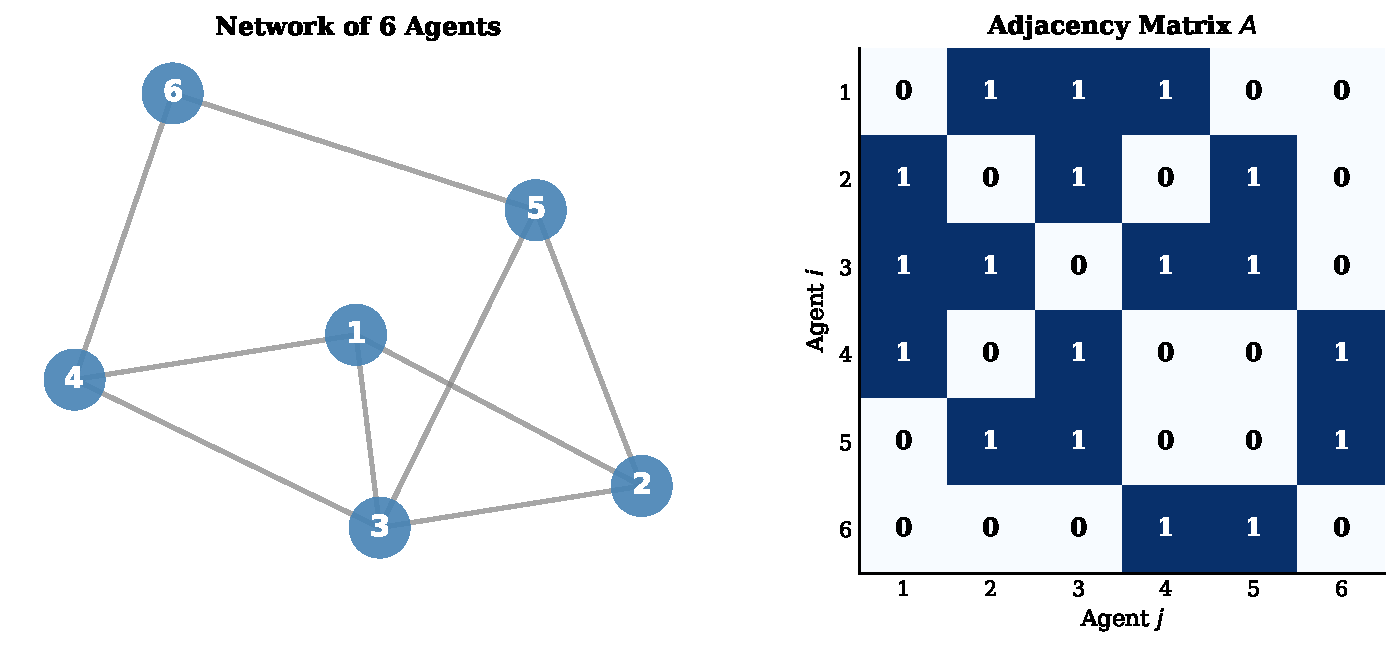
\includegraphics[width=\textwidth]{figures/network_example_chapter_3.pdf}
    \caption[Example network with six agents and corresponding adjacency matrix]{Example of a network with six agents (left) and the corresponding adjacency matrix (right). Nodes represent agents, and edges represent connections. The matrix encodes the network by entries equal to $1$ in each position $(i,j)$ where agent $i$ is connected to agent $j$, with $0$ indicating no connection. Note that this matrix is not normalised.}
    \label{fig:network_generation_example}
\end{figure}

For our population of $n$ agents we need to keep track of who is connected to whom, and we do this by building an adjacency matrix $\mat{G}$ whose element $G_{ij}$ encodes whether agent $i$ is connected to agent $j$. This encoding lets us efficiently compute neighbour-weighted averages such as the CoMO term.

Formally, we let the agent with index $i$ have a set of neighbours $N_i \subseteq \{1, 2, \ldots, n\}$ (assumed to be non-empty), and let $|N_i|$ denote its cardinality. We then define the network structure by the row-normalised adjacency matrix $\mat{G} \in \RR^{n \times n}$ where $G_{ij} = \frac{1}{|N_i|}$ if $j \in N_i$ (i.e., agent $j$ is a neighbour of agent $i$), and $G_{ij} = 0$ otherwise. Due to the row normalisation, $\sum_j G_{ij} = 1$ as all agents have at least one neighbour. With this definition, for any vector $\vect{x} = {(x_1, \ldots, x_n)}^\top$ we have ${(\mat{G}\vect{x})}_i = \frac{1}{|N_i|} \sum_{j \in N_i} x_j$, so $\mat{G}\vect{x}$ returns the vector of all neighbour-weighted averages in a single operation.

The adjacency matrix, along with the CoMO mechanism (see Section~\ref{sec:abm:como}), is used to introduce network effects into our model. When $G_{ij} > 0$, agent $j$ can influence agent $i$. For simplicity, we let all neighbours be equally close in terms of influencing each other.

For the results in this chapter, we construct the network using an Erd\H{o}s--R\'enyi random graph with connection probability $p = 0.1$ \parencite{ErdosRenyi1959, Gilbert1959}. The Erd\H{o}s--R\'enyi-based adjacency matrix is constructed by considering each possible connection between two agents independently. For each such possible connection (pair of agents $i$ and $j$), we create an undirected edge between the two agents with probability $p$, meaning that we have both $i \in N_j$ and $j \in N_i$. The result is a symmetric, unweighted adjacency matrix with $(n-1)p$ as the expected number of neighbours for each agent. For our simulations with $n = 100$ agents and $p = 0.1$ this gives an average of $9.9$ neighbours for each agent; for $n = 500$ it gives approximately $49.9$. After this, we row-normalise and retrieve the finalised adjacency matrix $\mat{G}$.


\subsection{The CoMO Mechanism}
\label{sec:abm:como}
In our simulations we include the CoMO mechanism of \textcite[Eqs.~1--2]{DahlFoldnesGronneberg2024} through the network-structured variant motivated in Section~\ref{sec:bg:social_comparison}, to capture the network effects of social comparison. The mechanism captures the potential of being ``left out'' of activity on social media to be costly. When friends have higher SMU, an individual loses out on social context and shared experiences, incurring a cost.

To formalise this for each agent $i$ at time $t$, we define their CoMO to be the positive gap between their own SMU and the average SMU of a reference group:

\begin{equation}
    c_{it} = \max\left(0, s_{i,t-1}^{\text{ref}} - s_{i,t-1}\right)
    \label{eq:como_main}
\end{equation}

For the results in this chapter, $s_{i,t-1}^{\text{ref}}$ will either be the population mean $\bar{s}_{t-1}$ or, when using an adjacency matrix, the adjacency-weighted neighbour mean ${(\mat{G}\vect{s}_{t-1})}_i = \sum_j G_{ij} s_{j,t-1}$. However, the mechanism allows for any reference group.

The CoMO mechanism introduces a cost to agents with an SMU smaller than the average in the reference group, and hence introduces network effects through peer comparison. In Chapter~\ref{chap:model}, we will provide a more thorough discussion of the CoMO mechanism.

\subsection{Update Rules}
\label{sec:abm:smu_dynamics}
Throughout the simulation, the agent's SMU should be evolving, and we need to specify how this evolution works. Our goal is to create semi-realistic behaviour in our agents, where each agent has habitual usage levels that they tend towards, but where daily use fluctuates. For example, an agent who typically uses social media for three hours might on some days use it for two hours or four hours, but a use of $10$ hours on any day should be extremely unlikely for this agent. We will later specify learning rules to let agents adapt to their environment.

We implement this type of behaviour through a mean-reverting first-order autoregressive (AR(1)) process. In an AR(1) process, we let each value of the process depend on the previous value and some noise. For a process with value $X_t$ at time $t$, $X_t = \phi X_{t-1} + \varepsilon_t$, where $\phi$ is called the persistence parameter and $\varepsilon_t$ is random noise. When $|\phi| < 1$, we say that the process is stationary, and we get a mean-reverting dynamic \parencite[Sec.~3.4, p.~53]{Hamilton1994}.

In our simulations we use such a mean-reverting AR(1) process where each agent's SMU fluctuates around their personal target level $\mu^s_i$. We write the update as:

\begin{equation}
    s_{it} = \phi \cdot s_{i,t-1} + (1 - \phi) \mu^s_i + \varepsilon^s_{it}, \quad \varepsilon^s_{it} \sim \N(0, {(\sigma^s_i)}^2)
    \label{eq:smu_ar1}
\end{equation}
Here, $\phi \in [0, 1)$ controls how quickly the agents revert to their target, and ensures the magnitude of changes in behaviour stays reasonable between each time step. In this way, agents are allowed to change behaviour, but still remain close to stable habitual behaviour of the past. The term $\mu^s_i$ pulls the agent towards its target SMU level. $\varepsilon^s_{it}$ is an error term that makes the process stochastic. For simplicity, we reuse the agent-specific scale $\sigma^s_i$ from initialisation rather than introducing a separate noise parameter. The target is updated through the learning rule, which allows the agents to adapt without extreme changes. We also clip the SMU values to $[0, 16]$ hours per day to ensure realistic values.

As with SMU, we need to define how agents' WB is updated throughout the simulation. We want each agent to have daily variation around a more stable trend. Well-being should be allowed to vary, as some agents are naturally happier than others, but we do not want overly large jumps from day to day. We also want the WB to be influenced directly by SMU and the CoMO effect. Each agent's use of social media should influence WB, and peer comparison should influence WB for agents below the average when the CoMO mechanism is active.

Combining these, we use the following update rule for the WB of agent $i$ at time $t$:

\begin{equation}
    y_{it} = \mu^y_i + \gamma_1 s_{it} + \gamma_2 \cdot c_{it} + \varepsilon^y_{it}, \quad \varepsilon^y_{it} \sim \N(0, {(\sigma^y_i)}^2)
    \label{eq:wb_basic}
\end{equation}
Here, $\mu^y_i$ is agent $i$'s baseline WB and $\varepsilon^y_{it}$ is the stochastic error term, while $\gamma_1$ and $\gamma_2$ measure the influence of SMU and CoMO on WB, respectively. Unlike with SMU, we model WB without persistence. We do this for simplicity, and because our interest is mainly in the contemporaneous effects of SMU and CoMO on WB\@.

Section~\ref{sec:abm:simpsons} extends this update rule to add delayed effects.

\subsection{Learning Rules}
\label{sec:abm:learning}
To make simulations more realistic, we implement learning to let agents adapt their behaviour based on the past. In real life, people generally adjust their behaviour based on experience. Thus, if an agent has a high SMU, leading to a low WB, we want them to be able to notice and change their behaviour accordingly. Similarly, if increasing SMU leads to increasing WB, agents should be given a way to notice this and adapt. This learning is crucial for the simulation, as it allows emergent behaviour to occur as agents adapt to their social environment.

In general we can allow the learning to target all attributes of the agent. For the simulations presented here, we let agents learn by updating their target SMU, $\mu^s_i$. Thus, the update also changes the magnitude of the influence on WB through SMU (and variables using SMU).

Agents update their target SMU using regression-based learning, as a way to move towards higher WB\@. This lets agents remember how their last days have been, what they did on those days, and update their behaviour based on any recent trends. For each agent we store a rolling window of the $W$ most recent $(s_{it}, y_{it})$ pairs. $W$ should not be very large, as learning based on more than just a few recent days is unrealistic. We estimate the slope of WB regressed on SMU on these pairs using OLS:
\begin{equation}
    \hat{\beta}_{it} = \frac{\sum_{\tau=1}^{W}(s_{i,t-\tau} - \bar{s}_{iW})(y_{i,t-\tau} - \bar{y}_{iW})}{\sum_{\tau=1}^{W}{(s_{i,t-\tau} - \bar{s}_{iW})}^2}
\end{equation}

Then, we update the target as follows:
\begin{equation}
    \mu^s_i \leftarrow \mu^s_i + \eta \cdot \text{clip}(\hat{\beta}_{it}, -5, 5)
\end{equation}

Here, $\eta$ is the learning rate, and we clip the estimated slope to avoid extreme values.

Thus, at each time $t$, each agent estimates the relationship between SMU and WB based on their own experience over the last few days, and moves their baseline behaviour slightly in the direction of increasing their own WB\@. This implementation of learning would be hard to model using standard statistical methods, but using ABMs makes this feasible.


\subsection{Design of Three Simulation Scenarios}
\label{sec:abm:dynamics}
For the results in this chapter, we simulate three different scenarios:

\begin{itemize}
    \item \textbf{Reference:} Baseline where all study types should recover the correct parameters. No network effects, neither CoMO nor adjacency.
    \item \textbf{CoMO:} Same as reference, but with the addition of population-mean-based CoMO with $\gamma_2 = -0.4$. No adjacency.
    \item \textbf{Network \& CoMO:} Same as reference, but with adjacency-weighted CoMO (still $\gamma_2 = -0.4$).
\end{itemize}

For each scenario, the simulation flow is as follows:

\begin{enumerate}
  \item Initialise $n$ agents with attributes (see Section~\ref{sec:abm:attributes}).
  \item For each time step $t = 1, \ldots, T$:
  \begin{enumerate}
    \item Compute CoMO\@.
    \item Update SMU and WB\@.
    \item Apply learning and update attributes.
  \end{enumerate}
\end{enumerate}

We simulate for $T = 500$ time steps, discard the first $B = 100$ time steps as burn-in, and store the results from the other time periods. In the case of the RCTs, the simulations are altered slightly (see Section~\ref{sec:abm:methods}). After simulating, we can apply the various research methods whose performance we wish to investigate. For an overview of the parameters used in the scenarios, see Table~\ref{tab:abm_main_params}.

\begin{table}[htbp]
\centering
\caption[Main parameter values used in simulations]{Main parameter values used in simulations.}
\label{tab:abm_main_params}
\begin{tabular}{llc}
\toprule
Parameter & Description & Value \\
\midrule
$n$ & Number of agents & 100 (500 for RCT) \\
$T$ & Number of days & 500 \\
$B$ & Burn-in period & 100 \\
$\phi$ & SMU persistence & 0.5 \\
$\gamma_1$ & SMU$\to$WB coefficient & $-0.5$ \\
$\gamma_2$ & CoMO$\to$WB coefficient & $-0.4$ \\
$\eta$ & Learning rate & 0.05 \\
$W$ & Learning window & 10 \\
\bottomrule
\end{tabular}
\end{table}

We note that the target estimand investigated in this chapter is the direct effect of own SMU on WB, with corresponding parameter $\gamma_1$. This scoping thus does not emphasise total effects. This simplification suffices for what we want to illustrate. The DGPs used are also illustrative, and not empirically calibrated. We use negative values for $\gamma_1$ and $\gamma_2$ for concreteness, but emphasise that the bias mechanisms found are due to the network effects. Thus, sign reversal would not change the conclusion. The simulations are therefore best interpreted as showing what \emph{can} happen in plausible networked worlds, not what \emph{does} happen in the SMU--WB literature.

%% Section 3.3: Implementation of Research Methods in Simulations
\section{Implementation of Research Methods in Simulations}
\label{sec:abm:methods}
To test our simulation results we implement three research methods that have been commonly used in the SMU--WB literature. For an explanation of how each method works and the assumptions they make, see Section~\ref{sec:intro:causal}. This section describes how each method is applied to the simulated data as a way to investigate the bias introduced by the network effects of the CoMO mechanism and adjacency implementation.

For the cross-sectional OLS (see Section~\ref{sec:intro:cross_sectional}), we need to use the output of the simulation at a single time step. We choose to use the last time step of the simulation, and hence regress WB on SMU across all $n$ agents at this time step. This gives an estimate of the cross-sectional association between SMU and WB at that time, which we interpret as an estimate of $\gamma_1$. The cross-sectional OLS estimator gives the answer that the approach most commonly used in empirical research (giving people a one-time survey asking about their SMU and WB) would give.

When it comes to the panel fixed effects estimation (described in Section~\ref{sec:intro:panel}), we use the data from the simulation after the burn-in period. Hence, we have $T - B = 400$ observations per agent. We first demean the data for each agent by subtracting their respective individual mean from their observations. Afterwards, we estimate the association between SMU and WB using the demeaned data, getting an estimate for $\gamma_1$. This procedure allows us to isolate within-agent variation over time, as it removes all time-invariant agent attributes from the estimation procedure.

To perform a simulated RCT (see Section~\ref{sec:intro:rct} for theory on RCTs), we need to decide on what intervention to simulate. We decide on the following treatment as an illustrative intervention. After the burn-in period, we assign $20\%$ of agents randomly to the treatment. The other $80\%$ of agents receive no treatment. The treated agents are capped in how much SMU they can have per day, to one hour per day. This cap is in effect for the rest of the simulation. The other agents (the ones in the control group) continue as normal, learning and modifying their behaviour as described in previous sections.

To be able to compare the treatment effect resulting from this simulation, we use the scaled estimator from Equation~\eqref{eq:rct_scaled}. This divides the difference in mean WB between the two groups by the difference in their mean SMU\@. Performing this scaling converts the treatment effect to a unit comparable to $\gamma_1$, which allows us to directly compare the estimated effect from the RCT with the estimates from cross-sectional OLS and the panel data with fixed effects. As in the cross-sectional OLS, we use the observations from the final time step for our RCT estimates.

The three methods are different in their implementations, which leads to large differences in their effective sample size (ESS). Cross-sectional OLS uses the $n$ observations at the final time step, and thus has an effective sample size of $n = 100$. The panel fixed effects use the temporal structure to draw on $n \times (T - B) = 40{,}000$ observations, giving them a substantially higher ESS than the other methods, though serial correlation in the AR(1) SMU process means the effective information is somewhat less than $40{,}000$ independent samples. The RCT, on the other hand, with its estimate based on the difference between the treated and control groups, achieves an effective sample size dominated by the smaller group. With $n = 100$ and $20\%$ treated, this leads to an ESS well below $100$, far lower than the other two.

To make the methods more comparable, we adjust the sample size for the RCT simulations by setting $n = 500$. With $20\%$ being assigned to the treatment, this brings the RCT's ESS closer to that of cross-sectional OLS, making noise from variation due to sample size more similar across the two methods. We choose not to make any adjustments to the panel fixed effects, as we consider the larger ESS an inherent advantage of the method. Making this adjustment, we can more easily interpret differences in bias as coming from network effects violating assumptions, and not just differences in sample size. We note that, as $p = 0.1$ is fixed, the increase in $n$ also increases the expected degree. Thus, this adjustment partly conflates method and density effects. Future work could perform a more careful analysis.

%% Section 3.4: Simulation Results
\section{Simulation Results}
\label{sec:abm:results}
We run and report results from simulations of the three scenarios. We run $M = 250$ simulations for each scenario and report Monte Carlo verification of bias estimates across these runs. We also plot the distributions of estimates to verify bias.

\subsection{Reference Scenario}
\label{sec:abm:reference}
Before investigating how the network effects introduced by CoMO and adjacency affect the results of the three research methods, we verify that the methods correctly recover the direct effect of SMU on WB, $\gamma_1 = -0.5$, when these mechanisms are absent. Hence, in the reference scenario we remove the CoMO effect on WB by setting $\gamma_2 = 0$ in Equation~\eqref{eq:wb_basic}. This yields the WB update equation:
\begin{equation}
    y_{it} = \mu^y_i + \gamma_1 s_{it} + \varepsilon^y_{it} = \mu^y_i - 0.5 \cdot s_{it} + \varepsilon^y_{it}
    \label{eq:wb_reference}
\end{equation}
The result is a simple DGP where the WB of an agent only depends on the agent's own SMU through $\gamma_1$, which the three research methods should be able to correctly recover.

\begin{table}[htbp]
\centering
\caption[Mean estimates of direct effect in the reference scenario]{Mean estimates of direct effect in the reference scenario across $M = 250$ Monte Carlo replications. True effect: $\gamma_1 = -0.5$.}
\label{tab:abm_reference}
\begin{tabular}{lcc}
\toprule
Method & Mean Estimate & Relative Bias (\%) \\
\midrule
Cross-sectional OLS & $-0.489$ & $2.3\%$ \\
Panel Fixed Effects & $-0.500$ & $0.1\%$ \\
RCT & $-0.487$ & $2.7\%$ \\
\bottomrule
\end{tabular}
\end{table}

The results for the simulations in the reference scenario are reported in Table~\ref{tab:abm_reference}. They show that all three methods recover a good estimate of the true effect of SMU on WB\@. This is as expected, as the reference DGP satisfies the assumptions needed for the methods to give unbiased results. In particular, we see that cross-sectional OLS gives a mean estimate of $-0.489$, panel fixed effects gives $-0.500$, and the RCT gives $-0.487$. All three estimates are close to the true value $\gamma_1 = -0.5$, confirming that our simulations and estimation procedures are implemented correctly.

\begin{figure}[htbp]
    \centering
    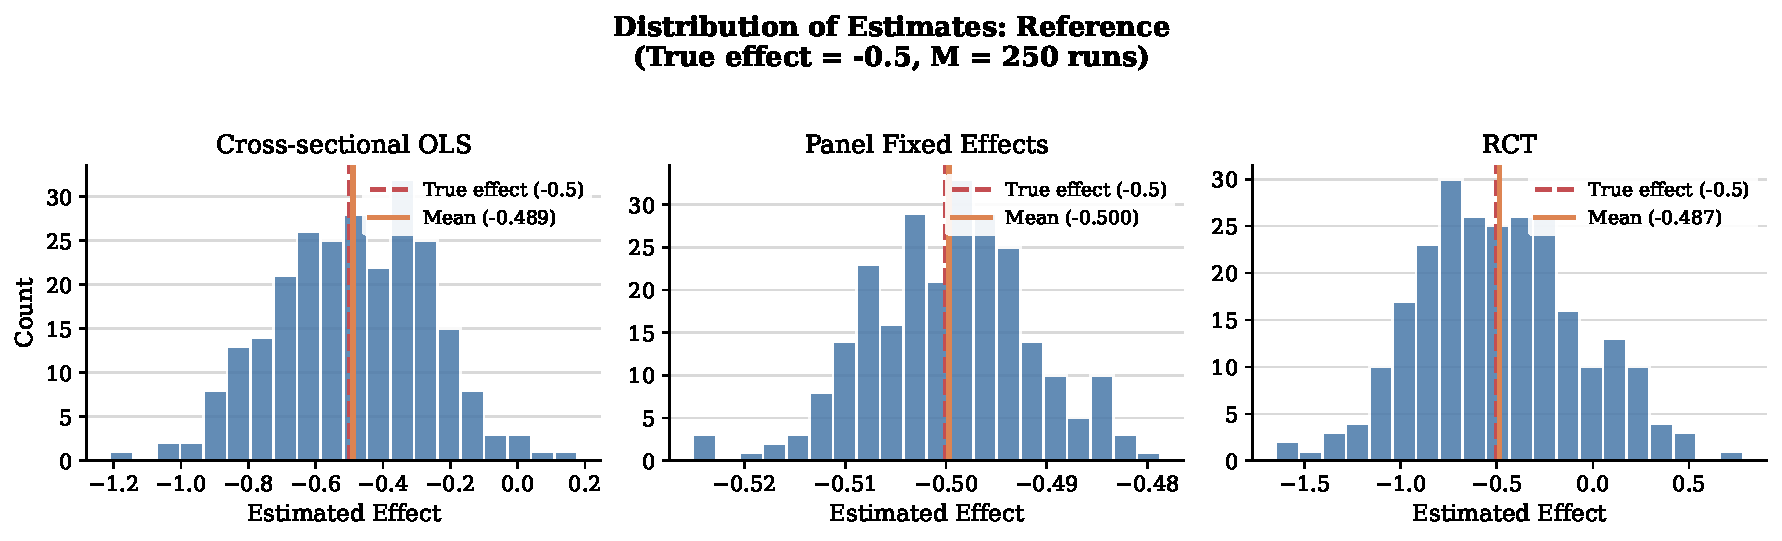
\includegraphics[width=\textwidth]{figures/abm_histogram_reference.pdf}
    \caption[Distribution of estimates for the reference scenario]{Distribution of simulation estimates for the reference scenario. All three methods correctly cluster around the true effect ($\gamma_1 = -0.5$, shown as vertical dashed line) when CoMO and agent adjacency are absent.}
    \label{fig:abm_histogram_reference}
\end{figure}

We also plot the distribution of the estimated values in Figure~\ref{fig:abm_histogram_reference}, where we see that the values are spread evenly around the true value. We note that the variation of the panel fixed effects is substantially smaller than that of the cross-sectional OLS and RCT\@. The RCT has slightly higher variation than OLS, despite comparable ESS\@. This is expected due to the additional SMU components in the scaled estimator (Equation~\eqref{eq:rct_scaled}) contributing some variance. The reference scenario establishes a baseline for comparison of the bias introduced by the CoMO and adjacency mechanisms in the other scenarios.

\subsection{CoMO Scenario}

In the second simulation we include the CoMO variable. With $\gamma_2 = -0.4$ this gives the following WB update equation:

\begin{equation}
    y_{it} = \mu^y_i + \gamma_1 s_{it} + \gamma_2 \cdot c_{it} + \varepsilon^y_{it}
     = \mu^y_i - 0.5 \cdot s_{it} - 0.4 \cdot c_{it} + \varepsilon^y_{it}
    \label{eq:wb_como}
\end{equation}

In this scenario the $c_{it} = \max(0, \bar{s}_{t-1} - s_{i,t-1})$ mechanism uses the population mean $\bar{s}_{t-1}$ as the reference group. This introduces network effects to the simulation through the peer comparison in the CoMO term. As the three research methods we are testing do not account for this in their structure, we expect them to yield biased results, which is exactly what we find in our simulations (see Table~\ref{tab:abm_como}): cross-sectional OLS gives a mean estimate of $-0.400$ with a bias of $20.1\%$, panel fixed effects yields $-0.391$ with a bias of $21.8\%$, and the RCT estimates $-0.371$ with a bias of $25.9\%$.

\begin{table}[htbp]
\centering
\caption[Mean estimates of direct effect in the CoMO scenario]{Mean estimates of direct effect in the CoMO scenario across $M = 250$ Monte Carlo replications. True effect: $\gamma_1 = -0.5$.}
\label{tab:abm_como}
\begin{tabular}{lcc}
\toprule
Method & Mean Estimate & Relative Bias (\%) \\
\midrule
Cross-sectional OLS & $-0.400$ & $20.1\%$ \\
Panel Fixed Effects & $-0.391$ & $21.8\%$ \\
RCT & $-0.371$ & $25.9\%$ \\
\bottomrule
\end{tabular}
\end{table}

Figure~\ref{fig:abm_histogram_como} shows the distribution of the estimates together with the true coefficient, showing a clear bias towards zero for all three methods. Hence, our results show that all three methods correctly identify the direction of the effect, but underestimate its magnitude when the CoMO mechanism is present. The bias towards zero is expected: when CoMO is introduced, agents who would otherwise benefit from low SMU are instead also affected negatively through the CoMO mechanism. Methods that do not take CoMO into account will fail to capture all of this negative association. With more negative association among the agents with lower SMU, the slope of the association flattens out, and we see a bias towards zero.

\begin{figure}[htbp]
    \centering
    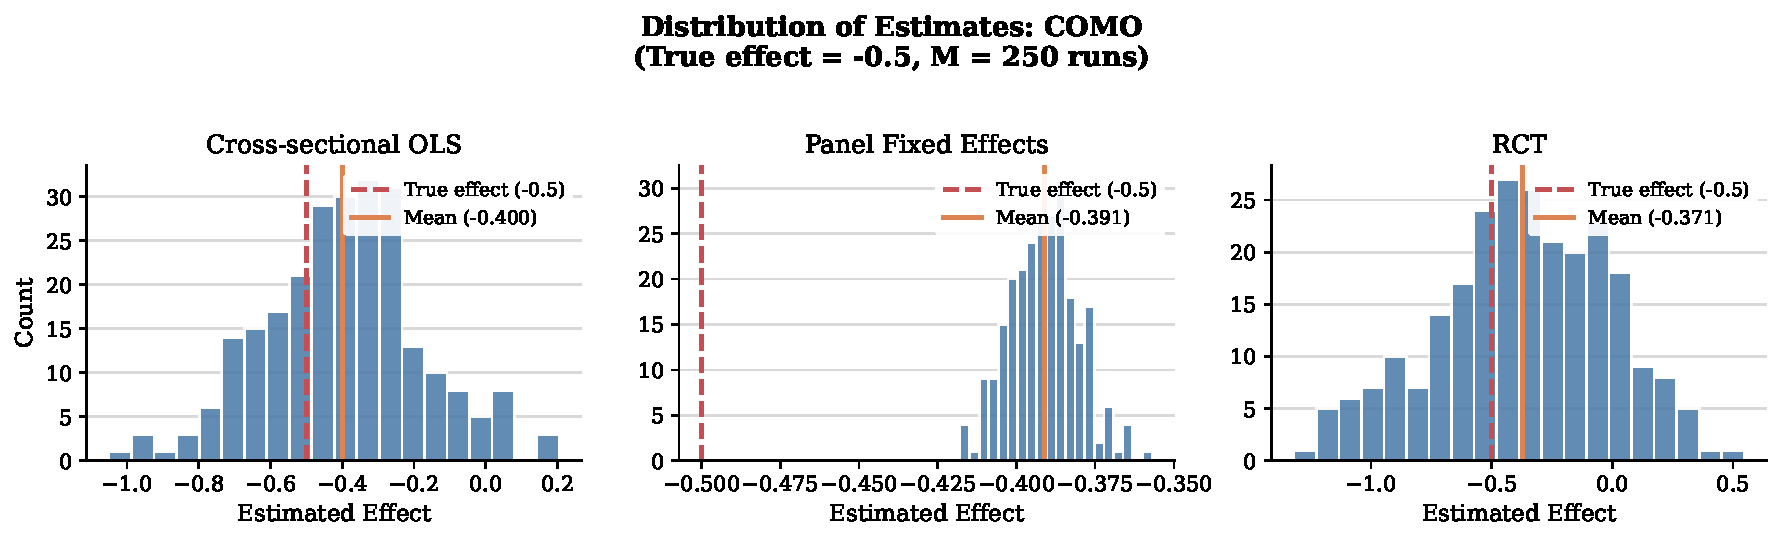
\includegraphics[width=\textwidth]{figures/abm_histogram_como.pdf}
    \caption[Distribution of estimates for the CoMO scenario]{Distribution of simulation estimates for the CoMO scenario. The true effect $\gamma_1 = -0.5$ is marked with a vertical dashed line. All methods show bias towards zero due to peer comparison through CoMO\@. As in the reference case, panel fixed effects has lower variance due to higher ESS.}
    \label{fig:abm_histogram_como}
\end{figure}

\subsection{Network \& CoMO Scenario}

The final scenario introduces both an adjacency matrix $\mat{G}$ and the CoMO mechanism. The adjacency matrix is constructed as an Erd\H{o}s--R\'enyi network with connection probability $p = 0.1$ as described in Section~\ref{sec:abm:network}. Using this matrix, we now calculate CoMO as $c_{it} = \max(0, {(\mat{G}\vect{s}_{t-1})}_i - s_{i,t-1})$ using the adjacency-weighted neighbour mean ${(\mat{G}\vect{s}_{t-1})}_i = \sum_j G_{ij} s_{j,t-1}$. Hence, we introduce local peer comparison, instead of the global comparison of the CoMO scenario.

With the same parameters as we used before, the WB update equation becomes:
\begin{equation}
    y_{it} = \mu^y_i - 0.5 \cdot s_{it} - 0.4 \cdot c_{it} + \varepsilon^y_{it}
    \label{eq:wb_network_como}
\end{equation}

The results are presented in Table~\ref{tab:abm_network_como}, and show the following: cross-sectional OLS yields a mean estimate of $-0.371$ with a bias of $25.7\%$, panel fixed effects produces $-0.391$ with a bias of $21.8\%$, and the RCT gives $-0.341$ with a bias of $31.9\%$.

\begin{table}[htbp]
\centering
\caption[Mean estimates of direct effect in the Network \& CoMO scenario]{Mean estimates of direct effect in the Network \& CoMO scenario across $M = 250$ Monte Carlo replications. True effect: $\gamma_1 = -0.5$.}
\label{tab:abm_network_como}
\begin{tabular}{lcc}
\toprule
Method & Mean Estimate & Relative Bias (\%) \\
\midrule
Cross-sectional OLS & $-0.371$ & $25.7\%$ \\
Panel Fixed Effects & $-0.391$ & $21.8\%$ \\
RCT & $-0.341$ & $31.9\%$ \\
\bottomrule
\end{tabular}
\end{table}

As with the CoMO scenario, we see correct sign estimation, but an underestimation of the effect magnitude. In practice, this means that we underestimate the harmful effects of SMU on WB\@. The RCT shows the largest bias here (under the network-density caveat from Section~\ref{sec:abm:methods}), and the increase in bias from the global to the local comparison is larger for the RCT than for OLS\@. When we change from global peer comparison to local, network effects become stronger. The smaller reference group increases the network influence, while the global comparison averages it out more. Local groups allow for larger magnitude and variation in effects.

\begin{figure}[htbp]
    \centering
    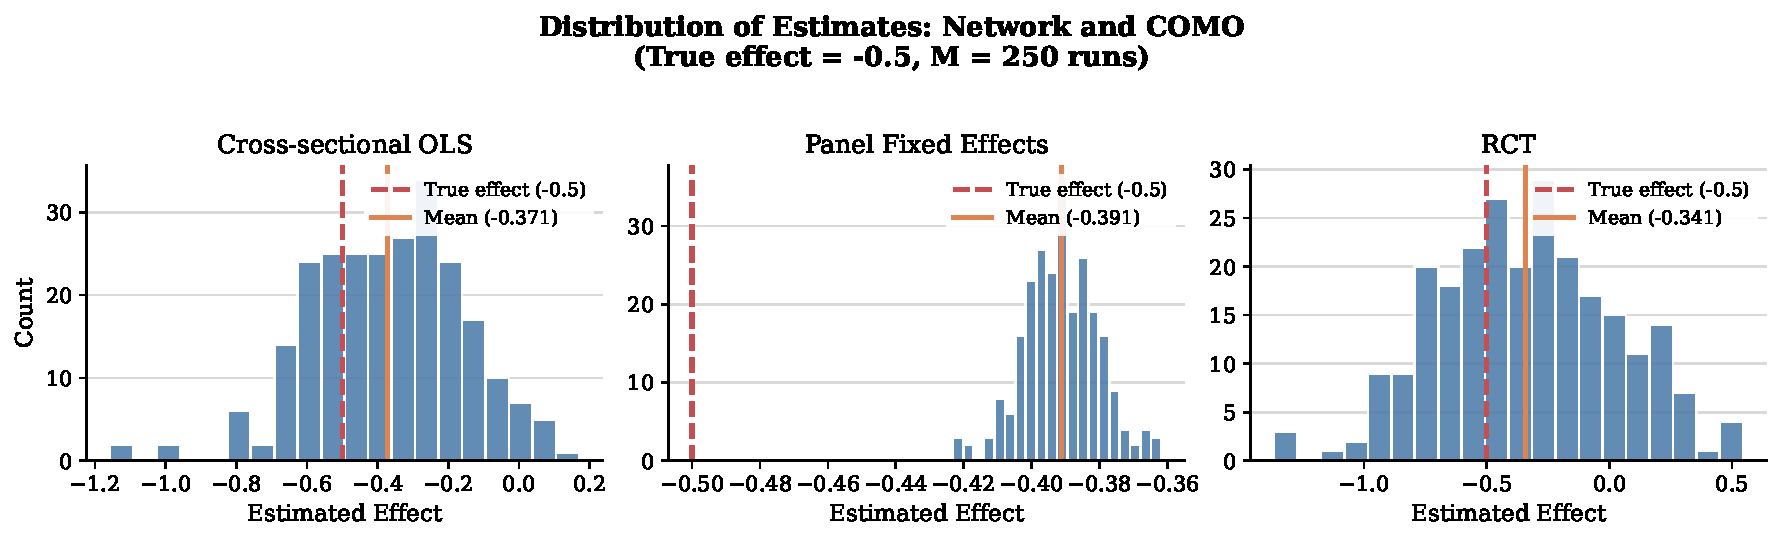
\includegraphics[width=\textwidth]{figures/abm_histogram_network_como.pdf}
    \caption[Distribution of estimates for the Network \& CoMO scenario]{Distribution of simulation estimates for the Network \& CoMO scenario using an Erd\H{o}s--R\'enyi graph with $p = 0.1$. The true effect $\gamma_1 = -0.5$ is marked with a vertical dashed line. All methods show bias towards zero, with the RCT having the largest bias.}
    \label{fig:abm_histogram_network_como}
\end{figure}

\subsection{Summary of Simulation Results}

We present a summary of the results across all three scenarios and research methods in Table~\ref{tab:abm_summary}. The table compares mean effect estimates, absolute bias, and relative bias.

\begin{table}[htbp]
\centering
\caption[Simulation results across all scenarios and methods]{Simulation results across all scenarios and methods. True effect: $\gamma_1 = -0.5$. Results based on $M = 250$ Monte Carlo replications per scenario.}
\label{tab:abm_summary}
\begin{tabular}{llccc}
\toprule
Scenario & Method & Mean & Abs.\ Bias & Rel.\ Bias (\%) \\
\midrule
Reference & Cross-sectional OLS & $-0.489$ & $0.011$ & $2.3\%$ \\
Reference & Panel Fixed Effects & $-0.500$ & $0.000$ & $0.1\%$ \\
Reference & RCT & $-0.487$ & $0.013$ & $2.7\%$ \\
\midrule
CoMO & Cross-sectional OLS & $-0.400$ & $0.100$ & $20.1\%$ \\
CoMO & Panel Fixed Effects & $-0.391$ & $0.109$ & $21.8\%$ \\
CoMO & RCT & $-0.371$ & $0.129$ & $25.9\%$ \\
\midrule
Network \& CoMO & Cross-sectional OLS & $-0.371$ & $0.129$ & $25.7\%$ \\
Network \& CoMO & Panel Fixed Effects & $-0.391$ & $0.109$ & $21.8\%$ \\
Network \& CoMO & RCT & $-0.341$ & $0.159$ & $31.9\%$ \\
\bottomrule
\end{tabular}
\end{table}

The results have some clear takeaways: in the reference scenario, the research methods work as intended, and are all able to capture the true effect of SMU on WB ($\gamma_1 = -0.5$). With $M = 250$ Monte Carlo replications, we observe very low bias for all three methods in the reference. In the CoMO and Network \& CoMO scenarios, all the effect estimates are biased towards zero under the specified DGPs, with the bias ranging from around $20\%$ to $32\%$. The RCT, often perceived as the most robust study type (see Section~\ref{sec:intro:rct}), shows the largest bias in our simulations (although the caveat from Section~\ref{sec:abm:methods} should be noted). This is due to the violation of the SUTVA assumption that its estimation rests on, coming from spillover effects from the treated group. When the agents in the treatment group reduce their SMU, this changes the reference level for the untreated agents, leading to biased estimates.

In Figure~\ref{fig:abm_forest}, we also provide a forest plot summary of the results with confidence bands to give a visualisation of the uncertainty from the Monte Carlo replications. This shows how the cross-sectional OLS and RCT have similar variation due to comparable ESS (with the RCT slightly wider), while the panel fixed effects method yields a much higher ESS, and thus a much lower variation.

\begin{figure}[htbp]
    \centering
    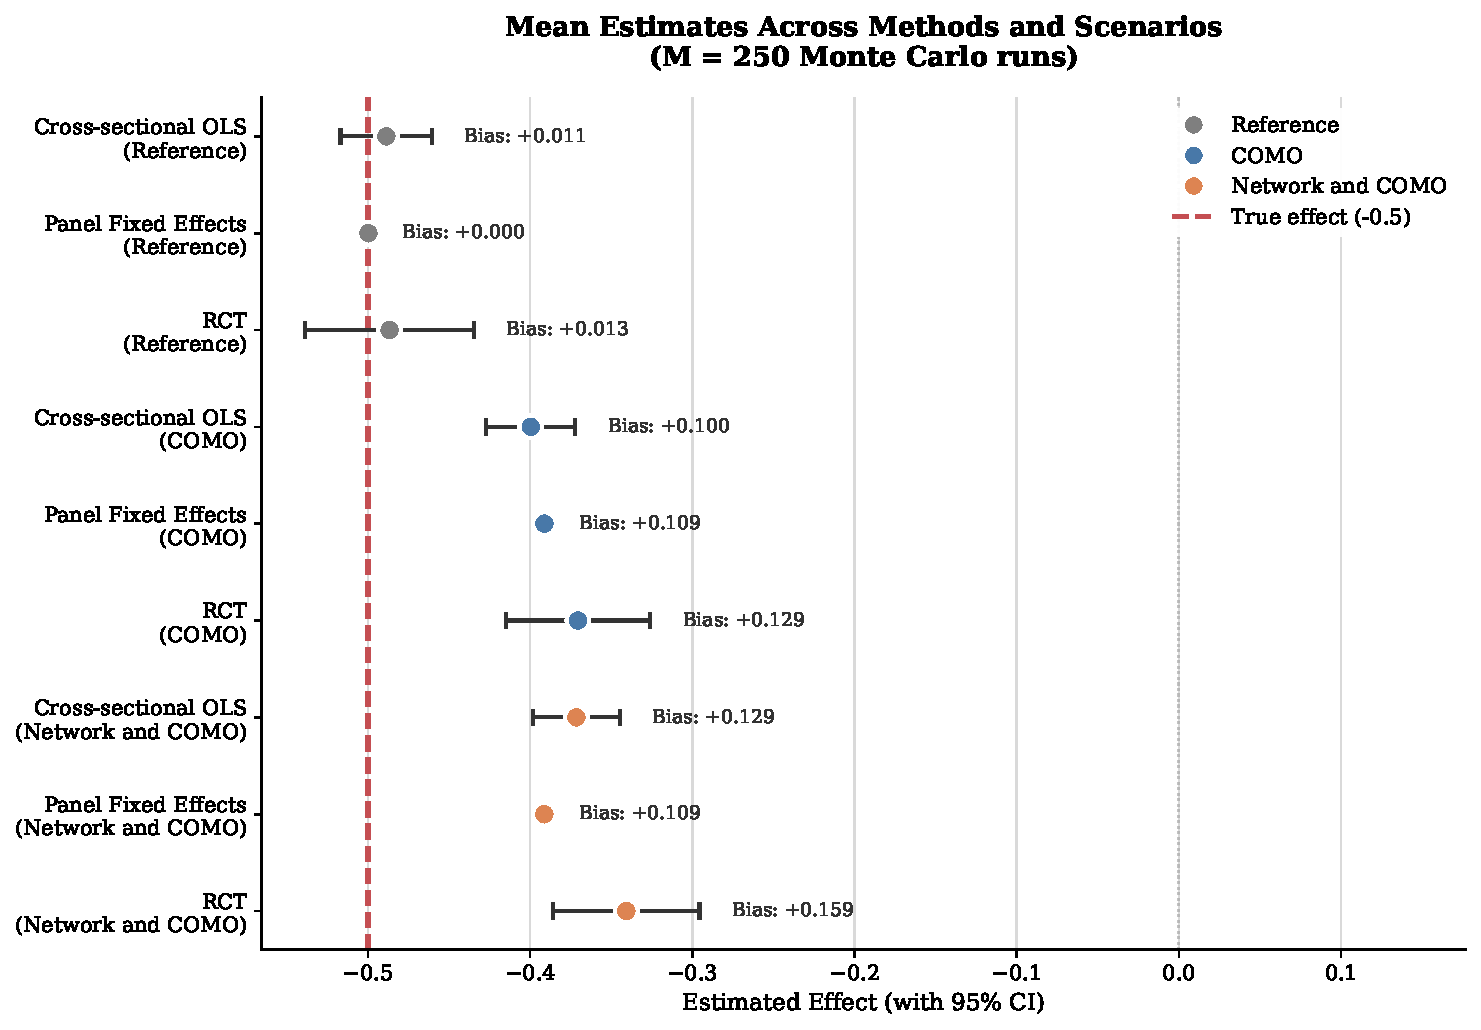
\includegraphics[width=\textwidth]{figures/abm_forest.pdf}
    \caption[Forest plot of mean estimates by method and scenario]{Forest plot of mean estimates for all methods and scenarios. Error bars show the $95\%$ CI of the mean across the Monte Carlo replications. The true effect $\gamma_1 = -0.5$ is marked with a vertical dashed line. All the methods exhibit bias in the non-reference scenarios.}
    \label{fig:abm_forest}
\end{figure}

%% Section 3.5: Demonstration of Simpson's Paradox
\section{Demonstration of Simpson's Paradox}
\label{sec:abm:simpsons}
The ABM framework we have implemented is general and allows for more complex simulations than the ones we have run above. ABMs have been proposed as a tool for simulating complex large-scale systems, including entire national economies \parencite{Farmer2009}. To demonstrate the versatility of the framework and how it can be used to investigate complex statistical phenomena, we use simulations to demonstrate Simpson's Paradox in the SMU--WB case.

In our case, we will demonstrate how, under plausible model assumptions, we can get a scenario where SMU has a negative influence on WB, and increased SMU leads to a decrease in WB on a population level, but where regressing WB on SMU at any given time $t$ will still yield a positive association. This showcases the intricacies involved in the research of the causal effect of SMU on WB\@.

\subsection{Background: What is Simpson's Paradox?}
\label{sec:abm:simpsons:bg}
Simpson's Paradox, first described by \textcite{Simpson1951}, is a phenomenon where a statistical association observed in aggregated data reverses or disappears when the data is partitioned into subgroups. The paradox is not just a statistical curiosity; it can occur in real data and thus has implications for causal inference. We provide an example of a classic version of Simpson's Paradox to explain the phenomenon.

\begin{example}[Classic Simpson's Paradox]
\label{ex:simpsons}
We construct a toy dataset for a study on the effectiveness of a treatment in two hospitals. In Hospital A, mostly severe cases are treated, while in Hospital B there are mostly mild cases:

\begin{center}
\begin{tabular}{lccc}
\toprule
 & Hospital A & Hospital B & Combined \\
\midrule
Treated patients ($n$) & 1{,}000 & 100 & 1{,}100 \\
Treatment success rate & $40\%$ & $90\%$ & $44.5\%$ \\[4pt]
Control patients ($n$) & 100 & 1{,}000 & 1{,}100 \\
Control success rate & $30\%$ & $80\%$ & $75.5\%$ \\
\midrule
Treatment effect & $+10\%$ & $+10\%$ & $-31\%$ \\
\bottomrule
\end{tabular}
\end{center}

Here we have constructed our toy data such that the treatment is beneficial in each hospital separately ($+10\%$ in both), but still appears harmful in total when we aggregate the data ($-31\%$). The effect stems from the unequal allocation between the two hospitals. Hospital A treats more serious cases (low baseline success rates), and contains the majority of treated patients. Hospital B, on the other hand, mostly treats milder cases, but contains most of the control patients. When aggregating, this leads to the treated group being dominated by the harder cases of Hospital A, while the control group contains mostly the easier patients from Hospital B, leading to a reversal of the observed association.
\end{example}

To not be confused by Simpson's Paradox we need to employ careful causal reasoning. The correct analysis of a problem depends on its causal structure. In the language of causal inference: if a hospital is a confounder (with an effect on both treatment assignment and outcomes, as it is in Example~\ref{ex:simpsons}), we need to condition on it. However, if the hospital is a mediator (where the treatment affects the outcome through the hospital choice), we should not. The logic of when to condition and when not to condition to land at the correct causal conclusion is discussed in \textcite[Ch.~6]{Pearl2009}.

There are multiple factors that make Simpson's Paradox a phenomenon that is particularly relevant to SMU--WB research:
\begin{itemize}
    \item \textbf{Aggregation happening over time}: Longitudinal trends and cross-sectional associations calculated at any given time point are not necessarily the same. Thus, it is possible to have a positive association between individual SMU and WB at any given moment (where those feeling better also have higher SMU), while still having increased SMU causing lower WB over time.
    \item \textbf{Network heterogeneity}: Due to network effects, associations within peer groups may be different from associations found at the population level due to homophily \parencite{McPherson2001} and peer influence.
    \item \textbf{Selection effects}: If there are selection effects present, where for example individuals with high SMU differ in some systematic way from those with low SMU, this can confound the relationship between SMU and WB\@.
\end{itemize}

\subsection{Adjusted Simulation Design}
\label{sec:abm:simpsons:design}
To demonstrate Simpson's Paradox, we add another component to our simulation structure, which we will call the \emph{delayed decline} mechanism. We include this mechanism to capture the idea that SMU might lead to short-term reward through entertainment and social connection, but long-term costs through reduced sleep quality and increased social comparison \parencites{Valkenburg2022}[Ch.~5]{Haidt2024}, see also Section~\ref{sec:bg:social_comparison}. An increased strength in the effect of CoMO on WB combined with this mechanism leads to the paradox arising.

The delayed decline mechanism alters the WB update rule by adding a temporal structure to how SMU influences WB\@. This is done through an impulse response function, which is a concept from time series analysis used to describe a system response over time to a one-time shock \parencite[Sec.~1.1, p.~5]{Hamilton1994}. In this way we can implement delayed consequences of SMU into our simulations. For our impulse response function we use a difference-of-exponential kernel, which is commonly used for modelling drug effects with varying onset and decay rates \parencite[Eq.~(9.11), p.~207]{Rosenbaum2016}.

The technical implementation adds these delayed decline terms to WB for each agent $i$ at each time $t$, computed as a sum of difference-of-exponentials weighted by past SMU values:
\begin{equation}
    \Delta y_{it}^{\text{delayed}} = \sum_{\tau=0}^{H-1} \left( \alpha_r e^{-\tau/\tau_f} - \alpha_p e^{-\tau/\tau_s} \right) s_{i,t-\tau}
    \label{eq:delayed_decline}
\end{equation}
Here, $\alpha_r$, $\alpha_p$, $\tau_f$, and $\tau_s$ are parameters controlling the reward and penalty scaling, influencing the magnitude and rapidity of decline of the additions made to WB\@. With a rapidly declining positive term and a slowly declining negative term we can capture immediate gratification with accumulating costs. In Figure~\ref{fig:delayed_decline_kernel}, we visualise the kernel with the parameter values used for the simulation. See Appendix~\ref{app:code:abm} for the parameter specifications. These values give a large immediate reward, with a decline spread out over time. Hence, at any given time, agents with a higher SMU get an immediate reward. This can dominate the negative direct and CoMO effects in the short term, while also incurring a future cost, which is how the paradox occurs.

\begin{figure}[htbp]
    \centering
    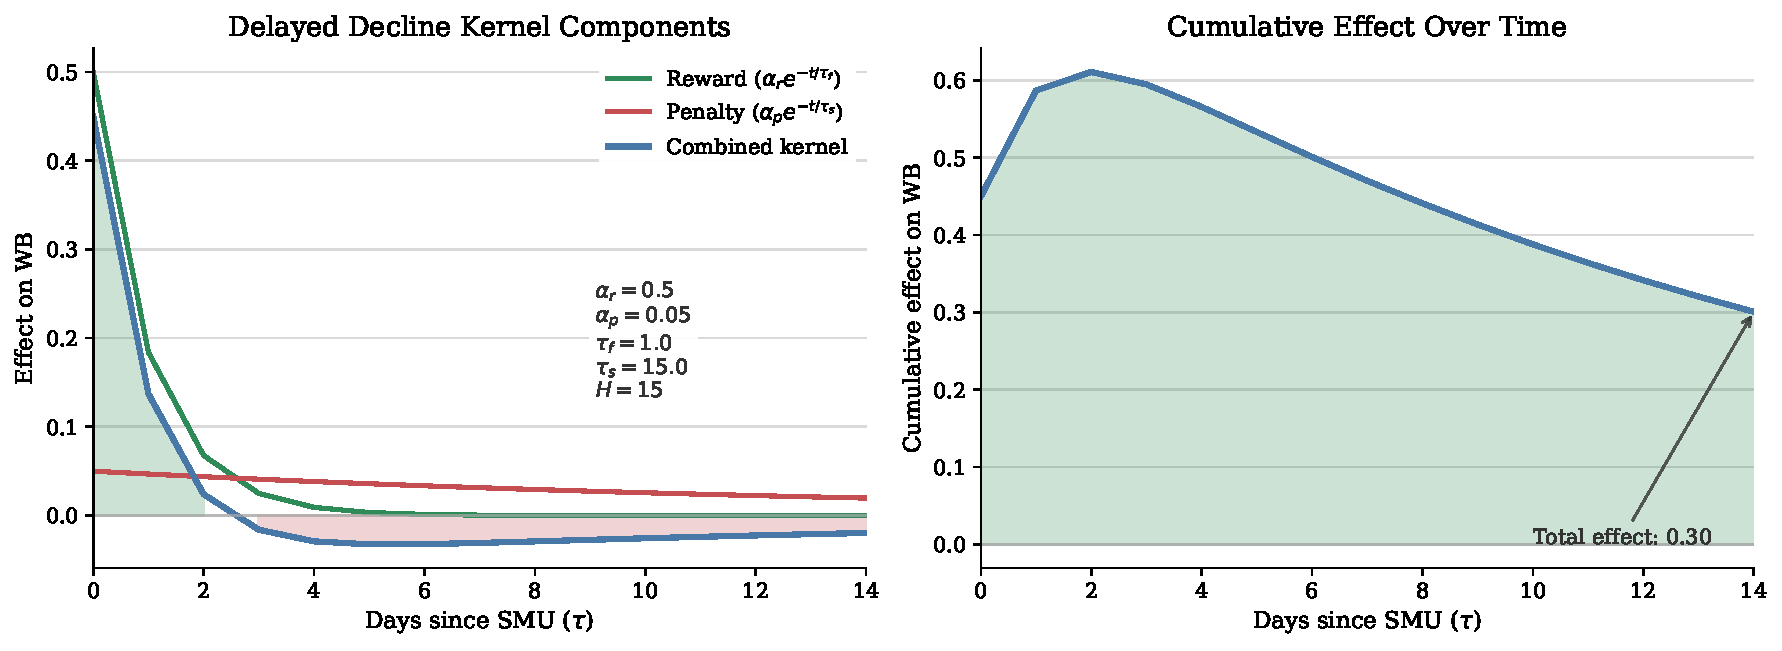
\includegraphics[width=\textwidth]{figures/delayed_decline_kernel.pdf}
    \caption[Delayed decline kernel used in the Simpson's Paradox simulation]{The delayed decline kernel used in the Simpson's Paradox simulation. The left panel shows the kernel effect, which is multiplied by each agent's SMU on the given day in the past. The green reward component declines rapidly due to $\tau_f = 1$, while the red penalty component declines slowly as $\tau_s = 15$. The red component is shown as positive here, but is subtracted from the green component in the blue combined kernel, which shows an immediate positive effect that quickly turns negative. The right panel shows the cumulative effect, assuming a constant unit of SMU over time. The kernel adds a positive cumulative effect, but the net effect after taking the direct effects of SMU and CoMO into account often becomes negative.}
    \label{fig:delayed_decline_kernel}
\end{figure}

To allow the delayed effects to have a clear influence at a population level, we use a larger population and more time steps than in the previous simulation. Additional parameter values are given in Appendix~\ref{app:code:abm}.

\subsection{Results and Interpretation}
\label{sec:abm:simpsons:results}
We visualise population mean SMU and WB throughout the simulation in Figure~\ref{fig:abm_simpsons_trends}. Here we see that after an initial volatile period (where the delayed effects kick in), the population moves to a decline in WB and increase in SMU\@.

\begin{figure}[htbp]
    \centering
    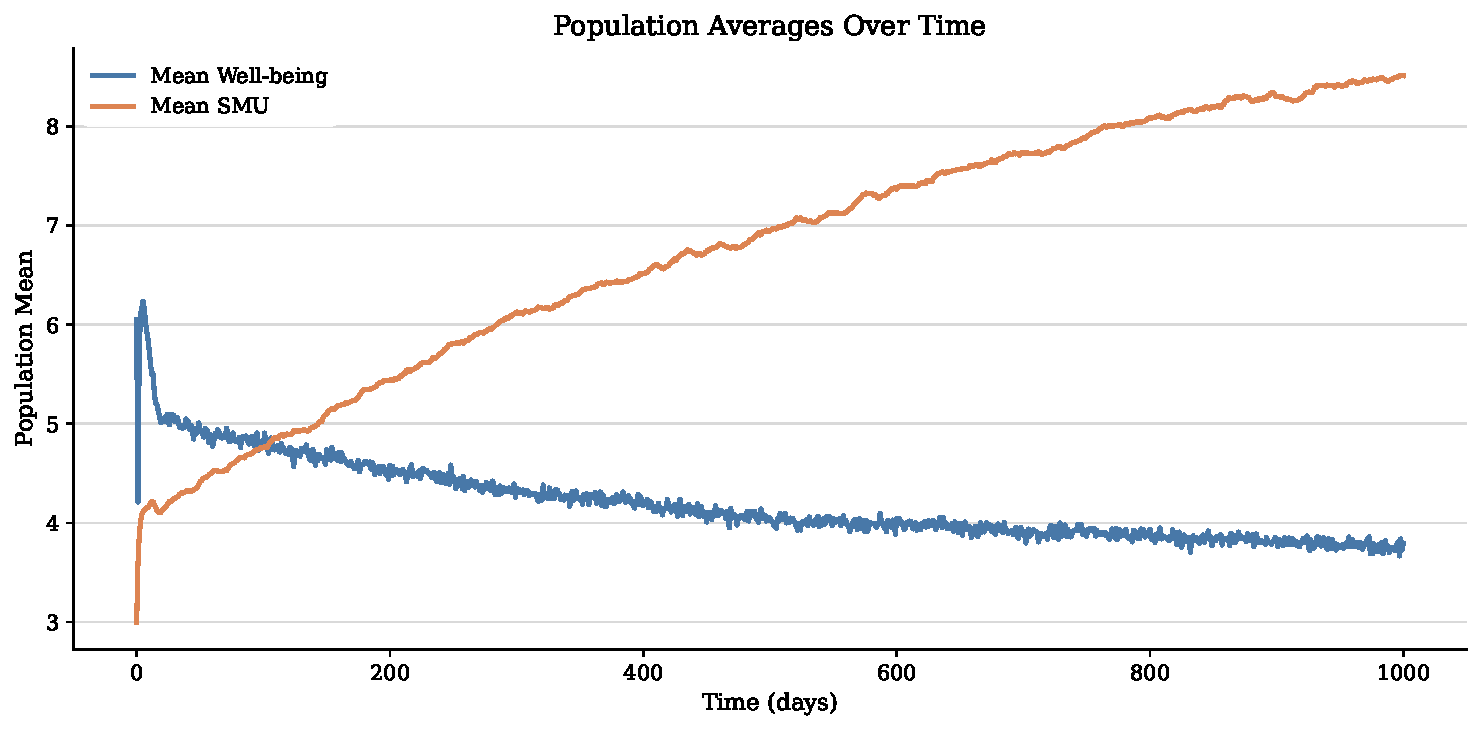
\includegraphics[width=\textwidth]{figures/abm_simpsons_trends.pdf}
    \caption[Average SMU and WB over time for the simulated population]{Average SMU and WB over time for the simulated population. The erratic start is caused by the delayed decline mechanism slowly kicking in.}
    \label{fig:abm_simpsons_trends}
\end{figure}

In Figure~\ref{fig:abm_simpsons_regressions} we visualise Simpson's Paradox. Here we again plot the mean WB of the population throughout the simulation period. We also show a scatter plot of the agents' SMU and WB values at times $t = 100$, $t = 500$, and $t = 900$, along with regression lines of simple linear regression using OLS\@. These all have positive slopes, showing how naive regression at any $t$ shows a different association than the one we observe at a population level.

\begin{figure}[htbp]
    \centering
    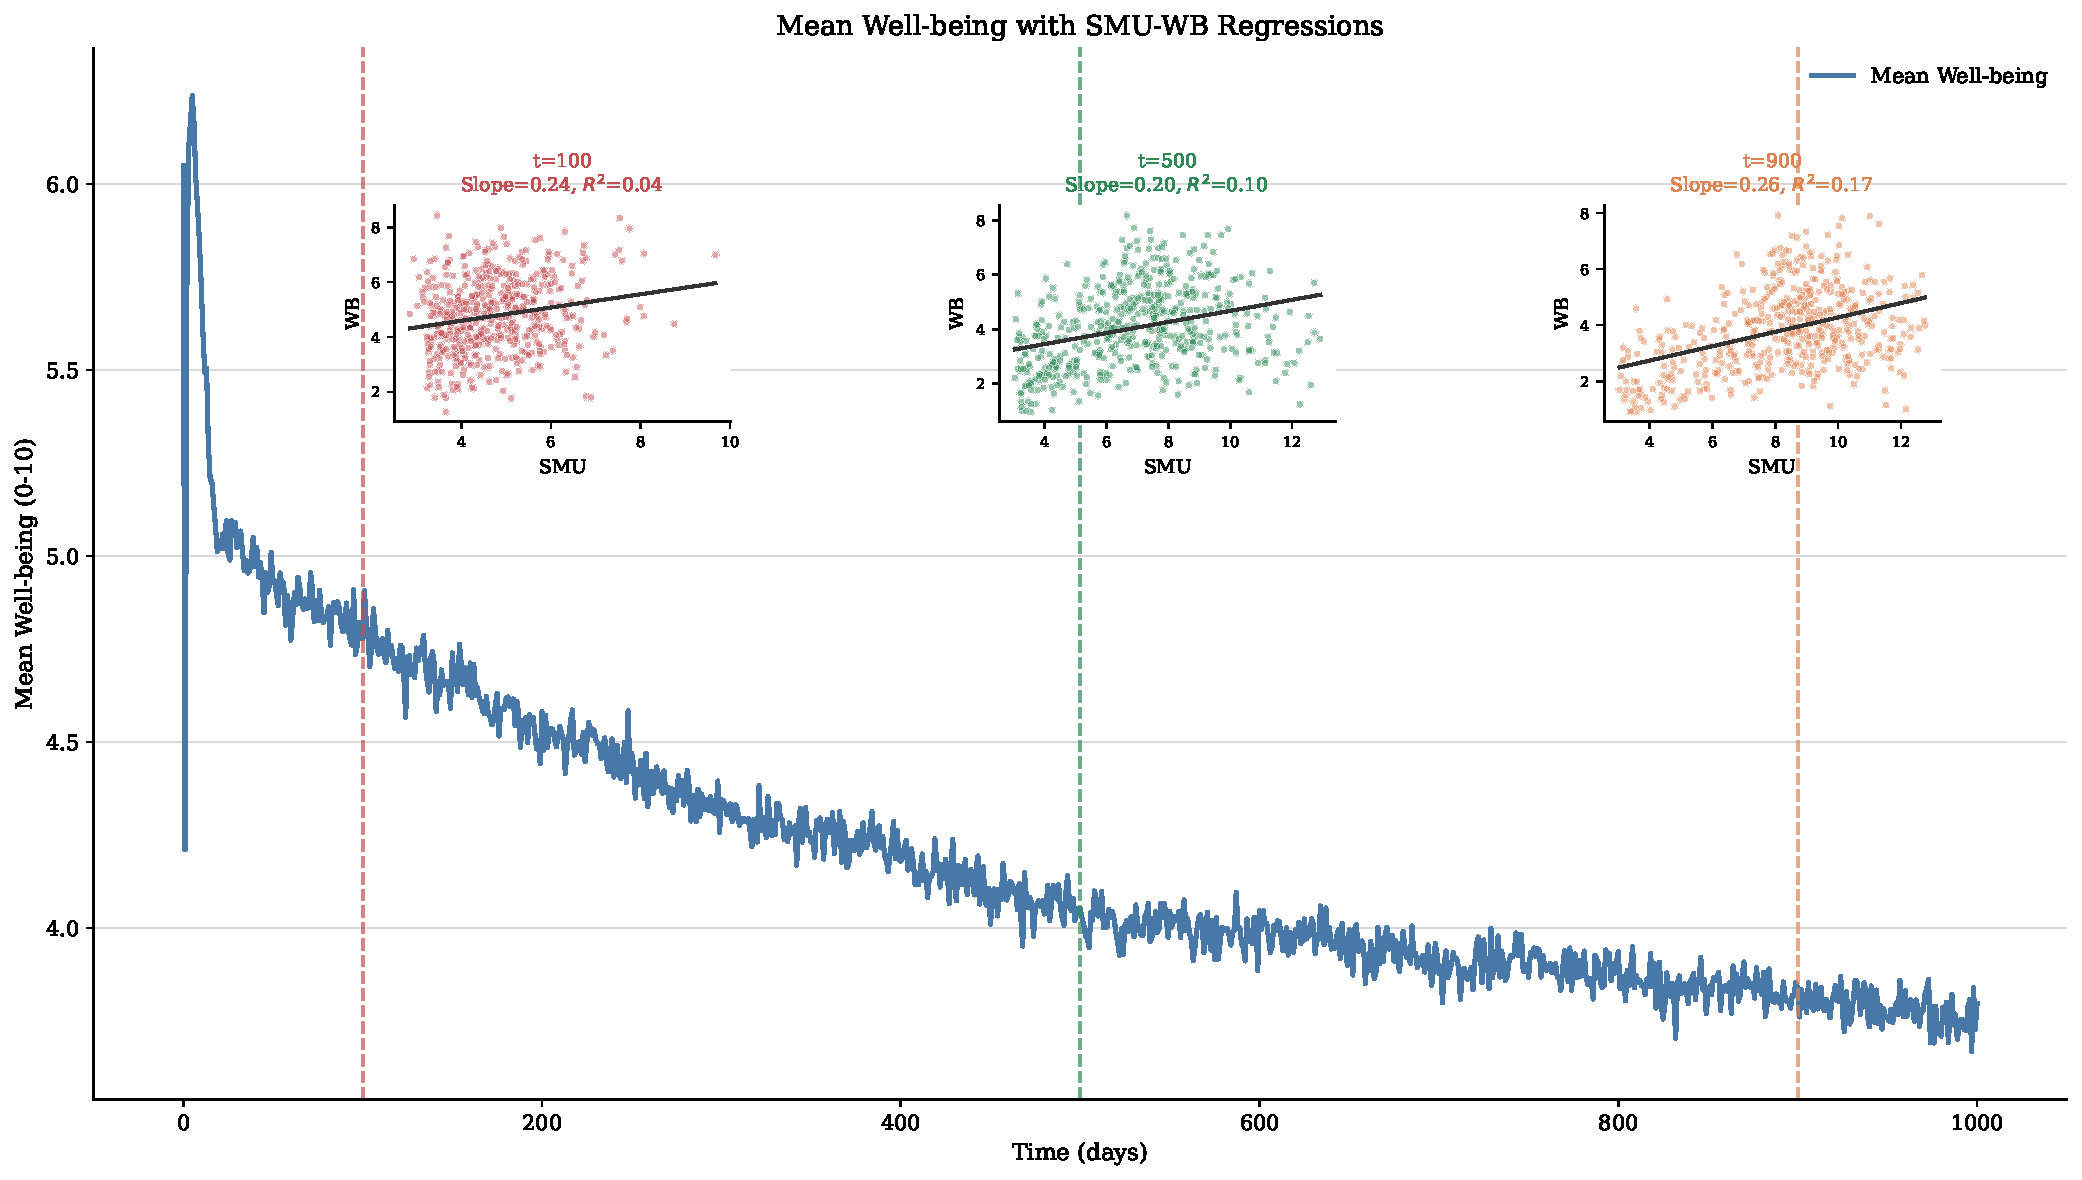
\includegraphics[width=\textwidth]{figures/abm_simpsons_regressions.pdf}
    \caption[Mean WB over time with cross-sectional SMU--WB regressions]{The blue line shows average WB over time for the simulated population. At $t = 100$, $500$, and $900$ we show scatter plots of all agents, with cross-sectional regression lines of the relationship between SMU and WB at each time point, all with positive slopes.}
    \label{fig:abm_simpsons_regressions}
\end{figure}

Hence, we see how the delayed decline mechanism combined with peer-comparison effects can lead to Simpson's Paradox. This implies a difficulty and a need to be very careful when interpreting results from the SMU--WB literature. From the point of view of a social scientist, we can imagine a researcher conducting a cross-sectional survey of a population at some time, finding a positive association between SMU and WB\@. From this, it would seem reasonable to conclude that SMU is harmless, or maybe even beneficial. Even a researcher who performed a longitudinal study, conducting multiple cross-sectional studies throughout time, would consistently find a positive association. However, as we can see when we look at the population-level trends, Simpson's Paradox is present, and the true causal effect is negative. Thus, we see that standard research methods might give very misleading results, and can even actively point in the opposite direction of the truth, when peer-comparison effects and temporal dynamics are present. This could have serious consequences when combined with large-scale policy implementations based on such findings.

In subsequent chapters we will focus on developing methods dealing with the bias shown in Section~\ref{sec:abm:results}.

%% Section 3.6: Discussion and Implications
\section{Discussion and Implications}
\label{sec:abm:implications}
Our simulation results showed biased estimates when the CoMO term and neighbour adjacency introduced network effects. We also showed how Simpson's Paradox led to further difficulties for causal interpretations. This section discusses the results with implications for the existing SMU--WB literature, and the path forward.

\subsection{Biased Results}

Why do we see biased results in our simulations? When we introduce the CoMO term with either population-level or neighbour-weighted social comparison, we are introducing network effects into our model, as well as an omitted regressor when it is not accounted for in the modelling.

The estimates made by cross-sectional OLS get biased because of violation of exogeneity in Assumption~\ref{ass:cross_sectional}. Here, CoMO will be an omitted regressor that is correlated with both SMU and WB\@.

For the OLS case, we can look formally at what is being calculated. The true DGP of our simulation is:

\begin{equation}
    y_i = \mu^y_i + \gamma_1 s_i + \gamma_2 \cdot c_i + \varepsilon_i
    \label{eq:ols_true_model_equation}
\end{equation}

The cross-sectional OLS regression estimates (omitting the CoMO variable):

\begin{equation}
y_i = \alpha + \tilde{\gamma}_1 s_i + u_i
\end{equation}

The OLS estimator is $\hat{\tilde{\gamma}}_1 = \frac{\Cov(s, y)}{\Var(s)}$. Substituting in the true model of Equation~\eqref{eq:ols_true_model_equation} for $y$ yields the standard omitted-variable bias formula \parencite[see][Eq.~(3.2.11), p.~60]{Angrist2009}, showing that $\hat{\tilde{\gamma}}_1$ converges in probability to:

\begin{equation}
\hat{\tilde{\gamma}}_1 \pto \gamma_1 + \gamma_2 \cdot \frac{\Cov(s, c)}{\Var(s)}
\end{equation}

For the CoMO term, agents with low SMU have higher values, so $\Cov(s, c) < 0$. As we also have $\gamma_2 < 0$, we get $\gamma_2 \cdot \frac{\Cov(s, c)}{\Var(s)} > 0$. As $\gamma_1$ is negative, this positive bias pulls it towards zero. This explains the bias towards zero, which is what we observe in our simulation results.

Assumption violations also lead to bias in the other two research methods. For the panel fixed effects we require uncorrelated errors and regressors across time in the strict exogeneity Assumption~\ref{ass:panel}. The network effects introduce time-varying confounding that cannot be controlled for by the fixed effects. The estimates made by RCTs rely on the SUTVA assumption (Assumption~\ref{ass:sutva}). When we cap SMU for the treatment group, this influences the reference level used in CoMO calculations for untreated agents as well. Hence, there is a spillover of the treatment into the control group, breaking the SUTVA assumption.

Mathematically, the SUTVA assumption translates into the RCT estimator $\hat{\tau} = \bar{y}^{\text{treated}} - \bar{y}^{\text{control}}$ being unbiased only when the outcomes of agents in the control group are unaffected by the treatment. However, when treated agents get their SMU reduced, this changes $\bar{s}^{\text{ref}}$ in the CoMO calculation for all agents (due to the network). Some of the outcome change of the treated group thus gets transferred to the control group, biasing $\hat{\tau}$ towards zero.

\subsection{Implications for Existing Literature}

As discussed in Section~\ref{sec:intro:motivation}, current research on SMU and WB has provided mixed results. We find it likely that network effects play a role. This has an important implication for the field of SMU--WB research in particular. Unlike other experimental fields, such as pharmaceutical trials, where patient outcomes are biologically independent (one patient taking a drug does not change drug efficacy in other patients), the individuals in SMU--WB research are involved in inherently networked systems. Thus, the SUTVA assumption underlying the gold standard of empirical research, RCTs, is violated. This leaves the field in a state where the causal question is still unanswered, which motivates the development of models taking network effects explicitly into account in subsequent chapters.

\subsection{Implications for Modelling of SMU--WB}

This chapter has shown that methods relying on individuals as independent units can be substantially biased when estimating causal effects in the presence of network effects. This motivates approaching the question through explicit modelling of network effects. In the next chapters, we will do just this. In Chapter~\ref{chap:model} we define a model for the influence of SMU on WB that explicitly includes network effects and the CoMO variable. In Chapters~\ref{chap:estimation} and~\ref{chap:monte_carlo} we use theory of maximum likelihood and two-stage least squares to find estimators for this model, and implement a Monte Carlo simulation study to validate the procedure. As we will see, under the assumption of our network-aware model, the estimators will produce unbiased estimates of the causal effects we are seeking. The model applies to a simpler DGP than the one used for our ABMs. In particular, it is static. Thus, we narrow the gap to ABMs without closing it. We discuss the remaining gap in Section~\ref{sec:discussion_conclusion:gap}.



% Chapter 4: The Recursive CoMO Model
%% Chapter 4: The Recursive CoMO Model

\chapter{The Recursive CoMO Model}
\label{chap:model}
In Chapter~\ref{chap:abm} we showed that under network effects, standard research methods give biased estimates of the causal effect of SMU on WB\@. This chapter introduces a model specification dealing with this issue by explicitly modelling the CoMO mechanism and the network structure. We present the model structure and equations, illustrate them with an example, and establish identification. This lays the theoretical framework for the estimation strategies we will employ in Chapter~\ref{chap:estimation}, where we develop both 2SLS and ML estimators.

When showing identification, we follow two paths, corresponding to the two estimators later developed. The first is to adapt the reasoning of \textcite{Bramoulle2009}, exploiting network structure for identification. This corresponds to the assumptions made for the 2SLS estimator. The second is to exploit the covariance structure of the model, due to the Gaussian likelihood, requiring the normality assumption underpinning the ML estimator. The identification results of this chapter (Propositions~\ref{prop:screen_identification},~\ref{prop:wb_identification}, and~\ref{prop:wb_ml_identification}) thus rely on existing tools, but are our own original derivations for the recursive CoMO model.

The modelling framework of this chapter addresses the central finding from Chapter~\ref{chap:abm} that network effects lead to bias. However, it does so on a static DGP, which makes identification and estimation tractable at a cost to realism. We discuss this simplification cost in Section~\ref{sec:model:discussion} and Section~\ref{sec:discussion_conclusion:gap}.

%% Section 4.1: Model Components
\section{Model Components}
\label{sec:model:components}
To make a model taking network structure into account, we first need a framework for modelling the relationship between SMU and WB\@. We do this by providing an equation for each, with a \emph{recursive} structure connecting them together, meaning that we let SMU influence WB, but not the other way around. The model also needs to take into account a network of $n$ individuals, with connections among the individuals. As we will see, we do this by a row-normalised adjacency matrix $\mat{G}$ (see Definition~\ref{def:row_normalised} and Section~\ref{sec:bg:networks} for theory on the adjacency matrix).

For the modelling of SMU and WB itself, we let each individual $i$ have the following variables:
\begin{itemize}
    \item Observed social media use $s_i$
    \item Observed well-being $y_i$
\end{itemize}

As in Chapter~\ref{chap:abm}, we let observed SMU be measured in hours per day, and observed WB be a continuous scale from $0$ to $10$. Each individual also has a set of neighbours (friends) $N_i \subseteq \{1, \ldots, n\}$, with these connections being represented in the adjacency matrix $\mat{G}$.

The model itself has a recursive structure, and consists of two equations modelling individuals' SMU and WB:
\begin{enumerate}
    \item \textbf{SMU equation}: An individual's SMU depends on peer SMU and exogenous factors.
    \item \textbf{WB equation}: An individual's WB depends on the individual's own SMU, the CoMO variable, peer WB, and exogenous factors.
\end{enumerate}

The recursive structure is advantageous as it allows the two equations to be estimated separately. Since SMU does not depend on WB, we can estimate the SMU equation based on only the observed $(\vect{s}, \mat{G})$. Similarly, the WB equation can be estimated from observed $(\vect{y}, \vect{s}, \mat{G})$ as it does not require any output from the SMU estimation.

%% Section 4.2: SMU Equation
\section{SMU Equation}
\label{sec:model:screen}
\subsection{Model Specification}

For the SMU equation we want to allow individual SMU to be realistic by including a baseline around which individuals vary, along with noise. We also want to include network effects, and do this through a term for the influence of the mean SMU of neighbours.

These components build the following model for the SMU of individual $i$:
\begin{equation}
\label{eq:screen_time}
    s_i = \beta_0 + \beta_1 \sbar_i + u_i, \quad i = 1, \ldots, n
\end{equation}

Here,

\begin{itemize}
    \item $\beta_0$ is a coefficient for baseline SMU
    \item $\beta_1$ is a coefficient that captures the peer influence on SMU $\sbar_i$, where $\sbar_i = \frac{1}{|N_i|}\sum_{j \in N_i} s_j = (\mat{G}\vect{s})_i$ is the average over the SMU of the peers of individual $i$ (defined through $\mat{G}$)
    \item $u_i \iid \N(0, \sigma_u^2)$ are independent normal error terms
\end{itemize}

For our purposes, it is also useful to have the equation in matrix form, as we will primarily use this later for parameter estimation. With $\vect{1} = (1, \ldots, 1)^\top$ denoting the vector of $n$ ones, $\vect{s} = (s_1, \ldots, s_n)^\top$ the vector of SMU values, and $\vect{u} = (u_1, \ldots, u_n)^\top$ the vector of errors, we can write the equation in matrix form as:

\begin{equation}
\label{eq:screen_matrix}
    \vect{s} = \beta_0 \vect{1} + \beta_1 \mat{G}\vect{s} + \vect{u}
\end{equation}

The focus point of this model is the $\beta_1$ parameter, which introduces the network effects. The parameter captures the degree of conformity to peers when it comes to SMU\@. When $\beta_1 > 0$, it draws the SMU of each individual towards the average of their peers. If $\beta_1 < 0$, individuals are non-conformist, and move in the opposite direction of their peer average. If $\beta_1 = 0$, the model does not include any influence from peers on individuals' SMU\@. Thus, this model can capture peer dynamics affecting individual SMU\@.

\subsection{Reduced Form with Distribution}

In preparation for estimation in Chapter~\ref{chap:estimation}, we follow the methods of \textcite[Sec.~2.3]{Bramoulle2009} and write the matrix version of the SMU equation in reduced form.

First, we rearrange terms in~\eqref{eq:screen_matrix}:

\begin{equation}
    \label{eq:screen_rearranged}
    (\mat{I} - \beta_1\mat{G})\vect{s} = \beta_0\vect{1} + \vect{u}
\end{equation}

We then make the following assumption:

\begin{assumption}[SMU Stability]
    \label{ass:screen_stability}
    The peer effect parameter satisfies $|\beta_1| < 1$.
\end{assumption}

Using Assumption~\ref{ass:screen_stability}, it follows from Proposition~\ref{prop:invertibility} in Section~\ref{sec:bg:sar} that $(\mat{I} - \beta_1\mat{G})$ is invertible, and we can thus write our reduced form of the equation:
\begin{equation}
\label{eq:screen_reduced}
    \vect{s} = (\mat{I} - \beta_1\mat{G})^{-1}\beta_0\vect{1}
             + (\mat{I} - \beta_1\mat{G})^{-1}\vect{u}
\end{equation}

We note that $\vect{u} \sim \N(\vect{0}, \sigma_u^2\mat{I})$ is the only random term in the reduced form equation~\eqref{eq:screen_reduced}, and so we can immediately write down the distribution of $\vect{s}$:

\begin{equation}
    \label{eq:s_distribution}
    \vect{s} \sim \N\left((\mat{I} - \beta_1\mat{G})^{-1}\beta_0\vect{1}, \;
    \sigma_u^2(\mat{I} - \beta_1\mat{G})^{-1}
    [(\mat{I} - \beta_1\mat{G})^{-1}]^\top\right)
\end{equation}

This follows from the following property of linear transformations of multivariate normal vectors: If $\vect{u} \sim \N(\vect{\mu}, \mat{\Sigma})$, then $\mat{A}\vect{u} + \vect{b} \sim \N(\mat{A}\vect{\mu} + \vect{b}, \mat{A}\mat{\Sigma}\mat{A}^\top)$, applied to $\N(\vect{\mu}, \mat{\Sigma}) = \N(\vect{0}, \sigma_u^2\mat{I})$.

%% Section 4.3: WB Equation
\section{WB Equation}
\label{sec:model:wellbeing}
\subsection{The CoMO Term}
\label{sec:model:como}
The introduction of our asymmetric, network-structured CoMO specification is a novel way of capturing peer effects within a structural network model. In Chapter~\ref{chap:abm} we showed how ignoring network effects of social comparison leads to bias in estimation of the effect of SMU on WB\@. The CoMO mechanism, introduced in the SMU--WB context by \textcite[Eqs.~1--2]{DahlFoldnesGronneberg2024} and motivated in Section~\ref{sec:bg:social_comparison}, captures the cost of missing out on shared context and experiences that individuals incur when their SMU is less than that of their peers. Thus, we are able to capture network effects in our model that would otherwise lead to biased estimates.

We define CoMO in our model as follows.

\begin{definition}[Cost of Missing Out]
    \label{def:como}
    The CoMO term for individual $i$ is:
    \begin{equation}
        c_i = \max(0, \sbar_i - s_i) = (\sbar_i - s_i)^+
    \end{equation}
\end{definition}

Here, $\sbar_i$ is the average SMU of the peers of individual $i$, as defined in Equation~\eqref{eq:screen_time}. In Figure~\ref{fig:como_function} we provide a graphical illustration of the CoMO effect.

\begin{figure}[htbp]
    \centering
    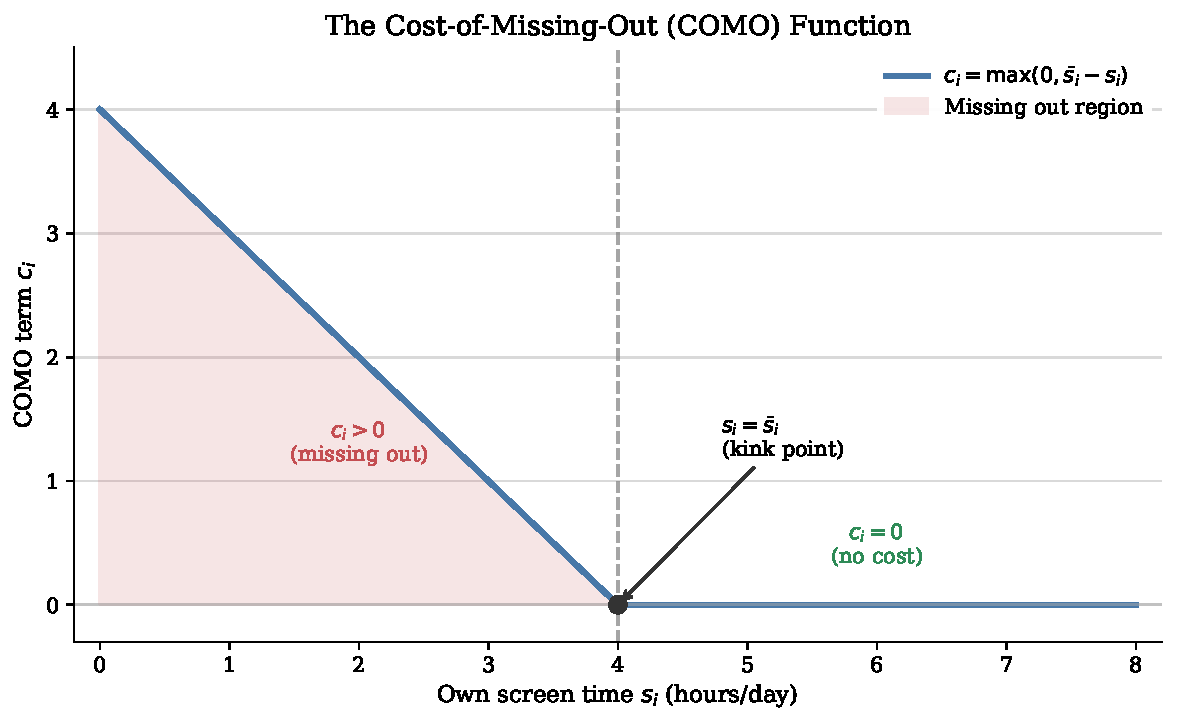
\includegraphics[width=0.8\textwidth]{figures/como_function.pdf}
    \caption[The CoMO function $c_i = \max(0, \sbar_i - s_i)$]{The blue line shows the CoMO function $c_i = \max(0, \sbar_i - s_i)$ for an individual with peer average $\sbar_i = 4$. When $s_i$ falls below the peer average $\sbar_i$, we get a positive CoMO term. When $s_i = \sbar_i$, we get a kink, showing the asymmetry of the CoMO mechanism.}
    \label{fig:como_function}
\end{figure}

The non-linear form of the CoMO term comes from our belief that individuals might pay a cost for having SMU below their peers, but that having SMU above the peer level does not necessarily give a direct positive effect on WB\@. Hence, we use the max operator, which leads to a mechanism that kicks in when $s_i < \sbar_i$. When an individual uses social media less than their peers, they experience the cost of missing out in proportion to the difference. When $s_i \geq \sbar_i$, i.e., when an individual uses social media at least as much as peers, there is no CoMO effect, $c_i = 0$. When the coefficient on CoMO in the WB equation is negative, CoMO reduces WB\@.

We also write the CoMO mechanism in vector notation:
\begin{equation}
    \vect{c} = (\mat{G}\vect{s} - \vect{s})^+ = \max(\vect{0}, \mat{G}\vect{s} - \vect{s})
\end{equation}
Here, the max is applied element-wise.

\subsection{Model Specification}

The WB part of the model is more complicated than the SMU part, as this is where we introduce the CoMO mechanism defined above. We want to let the network effects of neighbour SMU and WB influence the WB of each individual, as well as include a realistic baseline with random variation.

To include all these aspects, we use the following equation to model the WB of individual $i$:

\begin{equation}
\label{eq:wellbeing}
    y_i = \gamma_0 + \gamma_1 s_i + \gamma_2 c_i + \gamma_3 \ybar_i
        + \varepsilon_i, \quad i = 1, \ldots, n
\end{equation}

Here,

\begin{itemize}
    \item $\gamma_0$ is a coefficient for baseline WB
    \item $\gamma_1$ is a coefficient for the direct effect of individual SMU on WB
    \item $\gamma_2$ is a coefficient that captures the effect of the CoMO term $c_i$ on WB (Definition~\ref{def:como})
    \item $\gamma_3$ is a coefficient that captures the influence of peer WB, $\ybar_i$, on individual WB, where $\ybar_i = \frac{1}{|N_i|}\sum_{j \in N_i} y_j = (\mat{G}\vect{y})_i$ is the average WB of the peers of individual $i$ (defined through $\mat{G}$)
    \item $\varepsilon_i \iid \N(0, \sigma_\varepsilon^2)$ are independent normal error terms
\end{itemize}

A result of this specification is that the marginal effect of own SMU on WB is piecewise. This comes from the CoMO formulation $c_i = \max(0, \sbar_i - s_i)$. When holding the peer average $\sbar_i$ fixed, $\partial y_i / \partial s_i = \gamma_1 - \gamma_2$ when $s_i < \sbar_i$, and $\partial y_i / \partial s_i = \gamma_1$ when $s_i \geq \sbar_i$.

The $\gamma_1$, $\gamma_2$, and $\gamma_3$ parameters of the specification are the most interesting, and we provide a short interpretation of them here. $\gamma_1$ captures the direct effect of an individual's own SMU on their WB\@. Thus, if $\gamma_1 < 0$, a high SMU leads to lower WB, while $\gamma_1 > 0$ implies the opposite. For $\gamma_2$ we similarly have that the parameter controls the influence of the CoMO effect on individual WB\@. If $\gamma_2 < 0$, the CoMO effect has a negative influence on the WB of individuals who have less SMU than their peers. If $\gamma_2 = 0$, there is no social comparison, and when $\gamma_2 > 0$, this would imply a positive effect of lower SMU coming from peer comparison. Lastly, $\gamma_3$ controls the influence of peer WB on own WB\@. If $\gamma_3 > 0$, the positive WB of peers has a positive influence, while $\gamma_3 < 0$ would encode a cost of being around peers with high WB\@.

As with the SMU equation, we want a version in matrix form. Using the same notation as before, we introduce the design matrix
\begin{equation}
    \mat{X} = [\vect{1}, \vect{s}, \vect{c}]
\end{equation}
and let $\gammavec = (\gamma_0, \gamma_1, \gamma_2)^\top$ denote the parameter vector corresponding to the columns of $\mat{X}$. The matrix form of the WB equation is then:

\begin{equation}
    \label{eq:wellbeing_matrix}
    \vect{y} = \mat{X}\gammavec + \gamma_3\mat{G}\vect{y} + \vect{\varepsilon}
\end{equation}

\subsection{Reduced Form with Distribution}
For the purpose of model estimation in Chapter~\ref{chap:estimation}, we also write the WB equation in reduced form.

We first let $\Ay = \mat{I} - \gamma_3\mat{G}$. Then, rearranging Equation~\eqref{eq:wellbeing_matrix}, we get:

\begin{equation}
    \Ay\vect{y} = \mat{X}\gammavec + \vect{\varepsilon}
\end{equation}

We then make the following assumption:

\begin{assumption}[WB Stability]
    \label{ass:wb_stability}
    The peer effect parameter satisfies $|\gamma_3| < 1$.
\end{assumption}

Under Assumption~\ref{ass:wb_stability} it follows from Proposition~\ref{prop:invertibility} in Section~\ref{sec:bg:sar} that $\Ay$ is invertible, and we can thus write our reduced form of the equation:

\begin{equation}
    \label{eq:wellbeing_reduced}
    \vect{y} = \Ay^{-1}\mat{X}\gammavec + \Ay^{-1}\vect{\varepsilon}
\end{equation}

For the distribution of $\vect{y}$, the WB equation is more difficult to work with than the SMU equation. This is because the reduced form~\eqref{eq:wellbeing_reduced} includes $\vect{s}$ in two separate places in $\mat{X} = [\vect{1}, \vect{s}, \vect{c}]$: both through the direct effect of $\vect{s}$, and through $\vect{s}$ being part of the CoMO term $\vect{c} = \max(\vect{0}, \mat{G}\vect{s} - \vect{s})$. As the CoMO term is a non-linear function of $\vect{s}$ we do not get a straightforward unconditional distribution of $\vect{y}$.

However, if we condition on $\vect{s}$, both $\vect{s}$ and $\vect{c}$ will be fixed, and there only remains one random component: $\vect{\varepsilon} \sim \N(\vect{0}, \sigma_\varepsilon^2\mat{I})$. Thus, for the conditional case, we can apply the same linear transformation property as for the distribution of $\vect{s}$. Doing this, we get the following conditional distribution:

\begin{equation}
\label{eq:wellbeing_conditional_dist}
    \vect{y} \mid \vect{s} \sim \N\!\left(\Ay^{-1}\mat{X}\gammavec, \;\;
    \sigma_\varepsilon^2 \Ay^{-1}[\Ay^{-1}]^\top\right)
\end{equation}

The fact that we can get this conditional distribution comes from the recursive structure of our model. This distribution will be central when we develop an estimation strategy based on ML in Chapter~\ref{chap:estimation}. Since $\vect{s}$ is observed, we can condition on it directly and work with the multivariate normal likelihood of~\eqref{eq:wellbeing_conditional_dist}, avoiding the trouble caused by the non-linearity of the CoMO term.

%% Section 4.4: Illustrative Example
\section{Illustrative Example}
\label{sec:model:example}
Before moving to model assumptions and identification, we illustrate the various components of our model by working through an example with $n = 4$ individuals. The example also previews the network-lag intuition that underlies the identification argument in Section~\ref{sec:model:identification}.

\subsection{Network Structure}

To define the network structure, we need to decide what connections to make between the four individuals. We define the following relationships: individual 1 is friends with 2 and 3, individual 2 is friends with 1 and 4, individual 3 is friends with 1 only, and individual 4 is friends with 2 only. This creates an intransitive network, as 3 and 4 are not directly connected, but are still connected through other individuals. This feature of intransitivity will be used in Section~\ref{sec:model:identification}.

Based on these connections, the row-normalised adjacency matrix is:
\begin{equation}
    \mat{G} = \begin{pmatrix}
        0 & 1/2 & 1/2 & 0 \\
        1/2 & 0 & 0 & 1/2 \\
        1 & 0 & 0 & 0 \\
        0 & 1 & 0 & 0
    \end{pmatrix}
\end{equation}

In Figure~\ref{fig:network_example} we visualise this network along with the computed values below.

\begin{figure}[htbp]
    \centering
    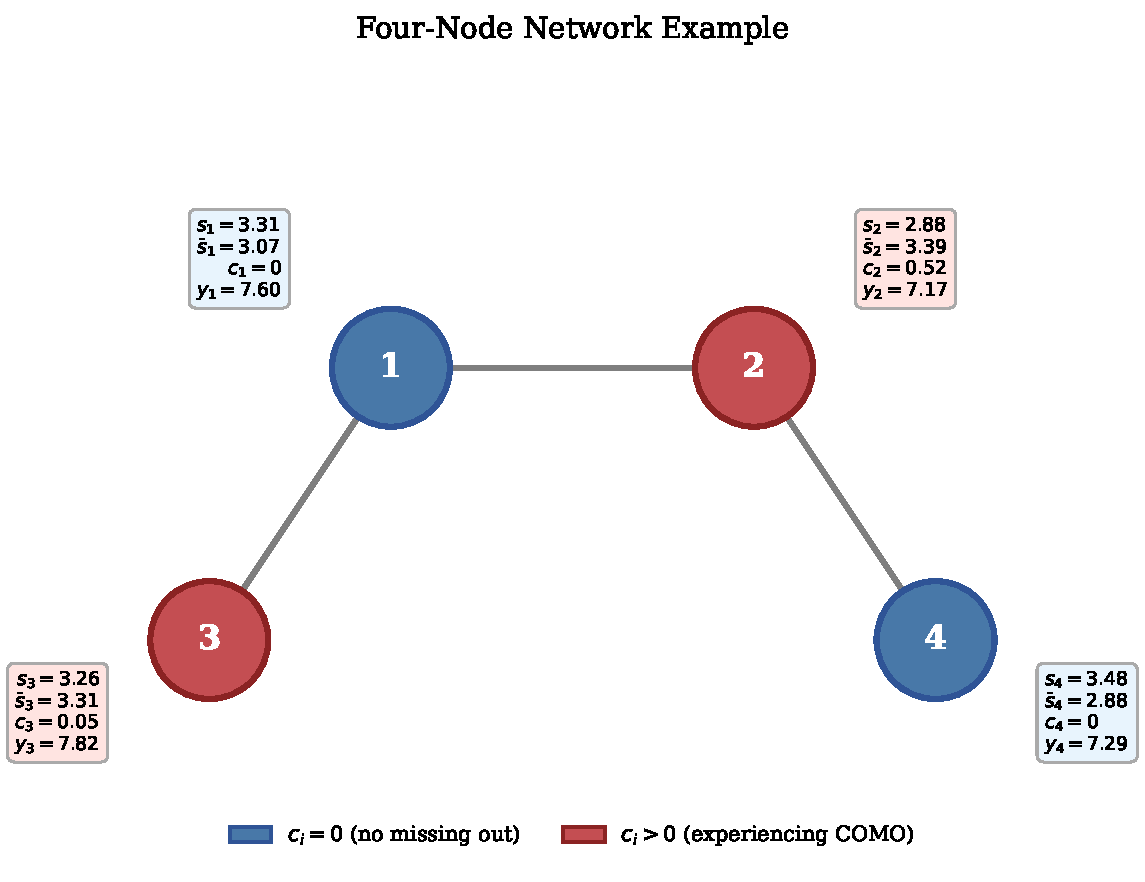
\includegraphics[width=0.85\textwidth]{figures/network_example_chapter_4.pdf}
    \caption[Four-node network example with SMU, peer average, CoMO, and WB]{Illustration of the four-node network used in the example. Nodes represent individuals, and edges represent network connections. For each node we show the values of individual SMU, $s_i$, the peer average $\sbar_i$, the CoMO term $c_i$, and the WB $y_i$. Individual 2 (red) experiences the largest CoMO effect, as they have SMU notably below their peer average.}
    \label{fig:network_example}
\end{figure}

\subsection{Computation of SMU, CoMO, and WB}

We suppose that the true parameters are $\beta_0 = 2.5$, $\beta_1 = 0.2$, $\sigma_u = 0.5$ ($\sigma_u^2 = 0.25$). This represents a baseline of 2.5 hours of daily SMU, a positive association with average peer use, and moderate variation. We also suppose that the errors are given as $\vect{u} = (0.2, -0.3, 0.1, 0.4)^\top$.

Using the reduced form $\vect{s} = (\mat{I} - \beta_1\mat{G})^{-1}(\beta_0\vect{1} + \vect{u})$ we can then calculate $\vect{s}$, and get (after matrix inversion):

\begin{equation}
    \vect{s} \approx (3.31, 2.88, 3.26, 3.48)^\top
\end{equation}

Using $\mat{G}$ we can then also calculate the peer averages of each individual:

\begin{equation}
    \mat{G}\vect{s} \approx (3.07, 3.39, 3.31, 2.88)^\top
\end{equation}

We use the peer averages to calculate the CoMO experienced by each individual:

\begin{align}
    c_1 &= \max(0, 3.07 - 3.31) = 0 \\
    c_2 &= \max(0, 3.39 - 2.88) = 0.52 \\
    c_3 &= \max(0, 3.31 - 3.26) = 0.05 \\
    c_4 &= \max(0, 2.88 - 3.48) = 0
\end{align}

In this example, individual 2 experiences the largest CoMO effect, as they use social media notably less than their peer average. Individual 3 experiences a negligible CoMO ($c_3 = 0.05$), while individuals 1 and 4 have $c_i = 0$.

Now, we suppose that the true parameters of the WB equation are $\gamma_0 = 7$, $\gamma_1 = -0.3$, $\gamma_2 = -0.5$, $\gamma_3 = 0.2$, and $\sigma_\varepsilon = 0.4$ ($\sigma_\varepsilon^2 = 0.16$), with observed variation $\vect{\varepsilon} = (0.1, -0.2, 0.3, -0.1)^\top$ for the individuals. This represents a high baseline WB of 7, with a negative effect of SMU and CoMO, a slightly positive effect of peer WB, and moderate variation.

These parameters give the following WB equation:

\begin{equation}
    y_i = 7 - 0.3 s_i - 0.5 c_i + 0.2 \ybar_i + \varepsilon_i
\end{equation}

Inserting our values in the reduced form of Equation~\eqref{eq:wellbeing_reduced} yields:

\begin{equation}
    \vect{y} \approx (7.60, 7.17, 7.82, 7.29)^\top
\end{equation}

We note that individual 2 has the lowest WB, partly caused by the CoMO term ($c_2 = 0.52$), which contributes $-0.5 \times 0.52 = -0.26$ to their WB\@.

\subsection{Network Lags and Friends-of-Friends}
\label{sec:model:network_lags}
A feature of the network that will become useful in Section~\ref{sec:model:identification} is that powers of $\mat{G}$ encode indirect network connections. Continuing our example above, we illustrate by computing $\mat{G}^2$:

\begin{equation}
    \mat{G}^2 = \begin{pmatrix}
        3/4 & 0 & 0 & 1/4 \\
        0 & 3/4 & 1/4 & 0 \\
        0 & 1/2 & 1/2 & 0 \\
        1/2 & 0 & 0 & 1/2
    \end{pmatrix}
\end{equation}

Even though $G_{14} = 0$, we have $(\mat{G}^2)_{14} = 1/4 > 0$. Thus, although individuals 1 and 4 are not directly connected, they are linked in $\mat{G}^2$ through their shared friend 2. A change in individual 4's SMU can only reach individual 1 through the network chain $4 \to 2 \to 1$. We call this an \emph{intransitive triad}: the presence of three individuals where $i$ connects to $j$ and $j$ to $k$ but $i$ does not connect to $k$. Such triads let friends-of-friends supply identifying variation beyond what direct friends provide. We will use this intuition in Section~\ref{sec:model:identification} to construct excluded instruments from network lags.

For this network, $\mat{I}$, $\mat{G}$, and $\mat{G}^2$ are also linearly independent, satisfying the formal condition we will use for the WB identification result.

Through this example we have shown how to construct the model variables for a fixed network, as well as how friends-of-friends connections appear through powers of $\mat{G}$. We now move on to the model assumptions required for identification and estimation.

%% Section 4.5: Model Assumptions
\section{Model Assumptions}
\label{sec:model:assumptions}
For identification and estimation, we need to make some assumptions on our model. In addition to Assumptions~\ref{ass:screen_stability} and~\ref{ass:wb_stability}, we make the following four assumptions for our recursive CoMO model:

\begin{assumption}[Error Independence]
\label{ass:error_indep}
The errors $u_i$ of Equation~\eqref{eq:screen_time} and $\varepsilon_j$ of Equation~\eqref{eq:wellbeing} are mutually independent for all
$i, j$.
\end{assumption}

\begin{assumption}[Error Normality]
\label{ass:normality}
The errors are drawn independently from two respective normal distributions: $u_i \iid \N(0, \sigma_u^2)$ and $\varepsilon_i \iid \N(0, \sigma_\varepsilon^2)$.
\end{assumption}

\begin{assumption}[Network Exogeneity]
\label{ass:network_exog}
The network $\mat{G}$ is exogenous, i.e., independent of the errors ($\vect{u}$, $\vect{\varepsilon}$) jointly.
\end{assumption}

\begin{assumption}[No Isolated Nodes]
\label{ass:no_isolates}
Every individual has at least one connection: $|N_i| \geq 1$ for all $i$. This ensures that $\mat{G}$ is row-stochastic, i.e., each row sums to one.
\end{assumption}

Assumption~\ref{ass:error_indep} is central to the estimation strategy of Section~\ref{sec:model:estimation_strategy}. When combined with the recursive structure, it ensures that $\vect{s}$ and $\vect{c}$ are exogenous in the WB equation, as we establish in Section~\ref{sec:model:id_wellbeing}.

In Assumption~\ref{ass:normality} we make a stronger assumption on the errors than \textcite[Sec.~2.1]{Bramoulle2009} do. They do not make any distributional assumptions on their errors, requiring only the moment condition $\E[\vect{\varepsilon} \mid \vect{x}] = \vect{0}$ (and allowing for heteroskedasticity and within-network dependence). We make a distributional assumption as well, as we need this for our ML estimation framework.

We also note that Assumption~\ref{ass:network_exog} is a strong assumption. It rules out mechanisms of network formation where friendships are based on unobserved factors that also affect outcomes, which is arguably not realistic. To give a clarifying example, suppose an unobserved personality trait, such as neuroticism, influences well-being. If individuals high on this trait also befriend each other more easily, this would lead to a network structure correlated with the error terms, violating the exogeneity assumption. This type of homophily, the tendency of similar individuals to flock together, is common in social networks \parencite{McPherson2001}. Relaxing this assumption is thus an important direction for future work.

%% Section 4.6: Identification
\section{Identification}
\label{sec:model:identification}
This section shows that our model is identified. By this we mean that the model parameters are uniquely recoverable given the distribution of observable data. In general, a model is identified if differences in parameter values lead to different observable distributions, i.e., we have an injective mapping from parameters to data distributions. If a model is not identified, there can be multiple parameter values that lead to the same observational distribution. Thus, no matter how much data we have, the parameters cannot be distinguished, and estimation would be fruitless. As we want to develop an estimation strategy in Chapter~\ref{chap:estimation}, we need to show that the parameters are identifiable. For the WB equation we provide two arguments: first we use networked instruments, following the logic of \textcite{Bramoulle2009} (Section~\ref{sec:bg:identification}), and then we show identification by exploiting the Gaussian likelihood. For the SMU equation we only provide the latter. The Gaussian likelihood approach draws on the SAR framework of Section~\ref{sec:bg:sar}.

\subsection{SMU Equation}

We start by showing that the SMU equation~\eqref{eq:screen_time} is identified. As constructed, the equation is a standard SAR model (Section~\ref{sec:bg:sar}) with only a constant as exogenous regressor.

With no individual-level covariates, the IV approach of \textcite{Bramoulle2009} does not apply. We will discuss this in more detail in Section~\ref{sec:est:screen_2sls}. We choose not to include covariates for simplicity. However, adding a covariate $x_i$ (for example, an individual's age or gender) with coefficient $\alpha$ would provide the exogenous characteristics needed to use network lags as instruments. A direct application of Proposition~\ref{prop:bramoulle} would then give us that $\beta_1$ is identified as long as $\mat{I}$, $\mat{G}$, and $\mat{G}^2$ are linearly independent and the non-cancellation condition $\beta_1\alpha \neq 0$ holds. If a contextual effect $\delta$ on $\bar{x}_i$ is included, the condition is $\delta + \beta_1\alpha \neq 0$.

Instead of taking this path, we have our simpler equation, for which identification follows from the distributional Assumption~\ref{ass:normality}. The idea of the approach is to use the fact that $\vect{s}$ is fully determined by its mean and covariance under normality. We can expand the precision matrix (the inverse of the covariance) as a polynomial in $\mat{G}$. This gives coefficients that identify $\beta_1$ and $\sigma_u^2$ under a condition of linear independence on the relevant matrices. When these are identified, we can use the mean to identify $\beta_0$.

\begin{proposition}[Identification of SMU Parameters]
\label{prop:screen_identification}
Under Assumptions~\ref{ass:screen_stability},~\ref{ass:normality},~\ref{ass:network_exog}, and~\ref{ass:no_isolates}, if the matrices $\mat{I}$, $\mat{G} + \mat{G}^\top$, and $\mat{G}^\top\mat{G}$ are linearly independent, then the parameters $(\beta_0, \beta_1, \sigma_u^2)$ are identified.
\end{proposition}

\begin{proof}
It suffices to show that any two triples of the parameters $(\beta_0, \beta_1, \sigma_u^2)$ that produce the same distribution of $\vect{s}$ are necessarily equal. By Assumption~\ref{ass:normality} we know that this distribution is multivariate normal. Thus, it is fully described by its mean and covariance. Our strategy is to first identify $\beta_1$ and $\sigma_u^2$ from the covariance, and then identify $\beta_0$ from the mean.

Using the result of Equation~\eqref{eq:s_distribution}, the covariance of $\vect{s}$ is
\[
    \mat{\Sigma}_s(\beta_1, \sigma_u^2)
    = \sigma_u^2 \As(\beta_1)^{-1}\As(\beta_1)^{-\top}.
\]
Here, $\As(\beta_1) = \mat{I} - \beta_1\mat{G}$ as before.

The precision matrix is well-defined, as $\As(\beta_1)$ is invertible under Assumption~\ref{ass:screen_stability} by Proposition~\ref{prop:invertibility}. Taking the inverse, we get that the precision matrix is given by
\[
    \mat{\Sigma}_s^{-1}
    = \frac{1}{\sigma_u^2}\As(\beta_1)^\top\As(\beta_1).
\]
We can expand the product to get
\[
    \As(\beta_1)^\top\As(\beta_1)
    = (\mat{I} - \beta_1\mat{G}^\top)(\mat{I} - \beta_1\mat{G})
    = \mat{I} - \beta_1(\mat{G} + \mat{G}^\top) + \beta_1^2 \mat{G}^\top\mat{G},
\]
yielding
\[
    \mat{\Sigma}_s^{-1}
    = \tfrac{1}{\sigma_u^2}\mat{I}
    - \tfrac{\beta_1}{\sigma_u^2}(\mat{G} + \mat{G}^\top)
    + \tfrac{\beta_1^2}{\sigma_u^2}\mat{G}^\top\mat{G}.
\]
So we have that the precision matrix is a linear combination of $\mat{I}$, $\mat{G} + \mat{G}^\top$, and $\mat{G}^\top\mat{G}$, with coefficients depending on $(\beta_1, \sigma_u^2)$.

We now suppose a different parameter pair $(\tilde\beta_1, \tilde\sigma_u^2)$ gives the same precision matrix. Then, subtracting the two precision matrices gives
\[
    \Big(\tfrac{1}{\sigma_u^2} - \tfrac{1}{\tilde\sigma_u^2}\Big)\mat{I}
    - \Big(\tfrac{\beta_1}{\sigma_u^2} - \tfrac{\tilde\beta_1}{\tilde\sigma_u^2}\Big)(\mat{G} + \mat{G}^\top)
    + \Big(\tfrac{\beta_1^2}{\sigma_u^2} - \tfrac{\tilde\beta_1^2}{\tilde\sigma_u^2}\Big)\mat{G}^\top\mat{G}
    = \mat{0}.
\]
The assumption of linear independence of $\mat{I}$, $\mat{G} + \mat{G}^\top$, and $\mat{G}^\top\mat{G}$ implies that the only solution is for each of the three coefficients to be equal to zero. But then the coefficient of $\mat{I}$ implies $\sigma_u^2 = \tilde\sigma_u^2$, the substitution of which into the coefficient of $\mat{G} + \mat{G}^\top$ then gives $\beta_1 = \tilde\beta_1$. The third coefficient is then also zero. This shows that both $\beta_1$ and $\sigma_u^2$ are identified.

We now need to show that $\beta_0$ is identified from the mean of $\vect{s}$. Using Equation~\eqref{eq:s_distribution} we get that $\E[\vect{s}] = \beta_0 \As(\beta_1)^{-1}\vect{1}$. 

We expand the term by applying the Neumann series for $\As(\beta_1)^{-1}$ from Proposition~\ref{prop:invertibility}. By the row-stochastic property of $\mat{G}$ (Assumption~\ref{ass:no_isolates}), $\mat{G}\vect{1} = \vect{1}$, and similarly $\mat{G}^k\vect{1} = \vect{1}$ by induction for all $k \geq 0$. Combining these gives
\[
    \As(\beta_1)^{-1}\vect{1}
    = \sum_{k=0}^{\infty} \beta_1^k \mat{G}^k \vect{1}
    = \sum_{k=0}^{\infty} \beta_1^k \vect{1}
    = (1 - \beta_1)^{-1}\vect{1},
\]

The final step follows as the geometric series converges to $(1-\beta_1)^{-1}$ by Assumption~\ref{ass:screen_stability}. The result gives us that $\E[\vect{s}] = \beta_0(1-\beta_1)^{-1}\vect{1}$. As $|\beta_1| < 1$ by Assumption~\ref{ass:screen_stability}, $1-\beta_1 \neq 0$. Since $\beta_1$ is identified, it follows that the mean uniquely determines $\beta_0$.
\end{proof}

\subsection{IV Identification of the WB Equation}
\label{sec:model:id_wellbeing}
The WB equation~\eqref{eq:wellbeing} contains multiple elements that make identification more challenging:

\begin{enumerate}
    \item To avoid Manski's reflection problem \parencite[Sec.~2]{Manski1993}, we need to ensure that $\vect{s}$, $\vect{c}$, and $\mat{G}\vect{y}$ are not collinear.
    \item The CoMO term $\vect{c} = \max(\vect{0}, \mat{G}\vect{s} - \vect{s})$ is a non-linear function of $\vect{s}$ and $\mat{G}\vect{s}$. We need to ensure that our model is identified despite this non-linearity.
    \item We need to identify the peer effect term $\mat{G}\vect{y}$, which is endogenous. By the reduced form $\vect{y} = (\mat{I} - \gamma_3\mat{G})^{-1}(\cdots + \vect{\varepsilon})$, we see that each $y_j$ depends on the error terms through the matrix inverse, which makes $\mat{G}\vect{y}$ correlated with $\vect{\varepsilon}$.
\end{enumerate}

In this section we address these by applying a network IV approach, based on the requirements of exogeneity and relevance of instruments in Section~\ref{sec:bg:iv}. In Section~\ref{sec:model:wb_ml_identification} we provide a strategy similar to the one we used for the SMU equation.

We adapt the identification logic of \textcite{Bramoulle2009}. This uses the network through friends-of-friends, whose characteristics only influence individual WB indirectly through the effect on direct friends. This makes them candidates for excluded instruments. As we have the non-linear CoMO term and no linear contextual terms in our recursive CoMO model, we cannot apply Proposition~\ref{prop:bramoulle} directly. However, standard IV machinery can still be applied, as our model is linear in its parameters with CoMO only entering conditionally on observed $\vect{s}$ through the regressor $\vect{c}$. It is thus possible to adapt the logic of \textcite{Bramoulle2009} to the recursive CoMO model. We do this in Proposition~\ref{prop:wb_identification} below, with a proof consisting of three steps: (i)~$\vect{s}$ and $\vect{c}$ are shown to be exogenous regressors, (ii)~$\mat{G}\vect{c}$ and $\mat{G}^2\vect{s}$ are shown to be valid excluded instruments for $\mat{G}\vect{y}$, and (iii)~this combined with a rank condition is shown to identify $\gamma_3$, with identification of $(\gamma_0, \gamma_1, \gamma_2)$ then following from standard regression moments.

\begin{proposition}[IV Identification of WB Structural Parameters]
\label{prop:wb_identification}
Let $\mat{W} = [\vect{1}, \vect{s}, \vect{c}, \mat{G}\vect{y}]$ collect the WB regressors and $\mat{Z} = [\vect{1}, \vect{s}, \vect{c}, \mat{G}\vect{c}, \mat{G}^2\vect{s}]$ collect the included exogenous regressors and the two excluded instruments. Under Assumptions~\ref{ass:screen_stability},~\ref{ass:wb_stability},~\ref{ass:error_indep},~\ref{ass:network_exog}, and~\ref{ass:no_isolates}, further suppose that $\mat{X} = [\vect{1}, \vect{s}, \vect{c}]$ has full column rank and that the rank condition
\[
    \rank(\E[\mat{Z}^\top\mat{W}]) = 4
\]
holds. Then the structural parameters $(\gamma_0, \gamma_1, \gamma_2, \gamma_3)$ are identified.
\end{proposition}

\begin{proof}
The argument proceeds in the three steps outlined above.

\textbf{Step 1: Exogeneity of $\vect{s}$ and $\vect{c}$, and full column rank of $\mat{X}$.}
This step lays the groundwork for the identification of $(\gamma_0, \gamma_1, \gamma_2)$. 

We begin with the reduced form~\eqref{eq:screen_reduced}, and note that $\vect{s}$ is a deterministic function of $(\vect{u}, \mat{G})$. By Assumptions~\ref{ass:error_indep} and~\ref{ass:network_exog}, we have $(\vect{u}, \mat{G}) \perp \vect{\varepsilon}$. So $\vect{\varepsilon}$ is independent of $(\vect{u}, \mat{G})$, and also of any function of $(\vect{u}, \mat{G})$, including $(\vect{s}, \mat{G})$. Hence, $\vect{\varepsilon}$ is also independent of $\vect{s}$, and we have established the conditional mean-zero property
\[
    \E[\vect{\varepsilon} \mid \vect{s}, \mat{G}]
    = \E[\vect{\varepsilon}] = \vect{0}.
\]
Similarly, the CoMO term $\vect{c} = \max(\vect{0}, \mat{G}\vect{s} - \vect{s})$ is a deterministic function of $(\vect{s}, \mat{G})$, and hence measurable with respect to the same conditioning information. As further conditioning on $\vect{c}$ adds no new information, we also have
\[
    \E[\vect{\varepsilon} \mid \vect{s}, \vect{c}, \mat{G}]
    = \vect{0}.
\]
Thus, $\vect{s}$ and $\vect{c}$ are exogenous regressors in the WB equation.

The condition of full column rank of $\mat{X} = [\vect{1}, \vect{s}, \vect{c}]$ is required to make $(\gamma_0, \gamma_1, \gamma_2)$ separately identified. The condition can fail in degenerate cases where the realised network and SMU vector make $\vect{c}$ collinear with $\vect{1}$ and $\vect{s}$. It is satisfied generically and is taken as a working assumption.

\textbf{Step 2: Validity of $\mat{G}\vect{c}$ and $\mat{G}^2\vect{s}$ as excluded instruments.}
We now show that $\mat{G}\vect{c}$ and $\mat{G}^2\vect{s}$ are valid excluded instruments by verifying exogeneity, exclusion, and relevance.

\emph{Exogeneity.} As both $\mat{G}\vect{c}$ and $\mat{G}^2\vect{s}$ are deterministic functions of $(\vect{s}, \mat{G})$, the argument from Step~1 applies. Conditioning on them adds no information beyond what $(\vect{s}, \mat{G})$ already does, so
\[
    \E[\vect{\varepsilon} \mid \vect{s}, \vect{c}, \mat{G}\vect{c}, \mat{G}^2\vect{s}, \mat{G}]
    = \vect{0}.
\]

\emph{Exclusion.} In the WB equation~\eqref{eq:wellbeing}, neither $\mat{G}\vect{c}$ nor $\mat{G}^2\vect{s}$ appears directly as a regressor. We note that $\mat{G}\vect{c}$ is a valid excluded instrument at the \emph{first} network lag. The non-linearity of the CoMO term is what makes this possible. In a standard fully linear SARX model, there are no excluded instruments at the first network lag.

\emph{Relevance.} We need to show that $\mat{G}\vect{c}$ and $\mat{G}^2\vect{s}$ are relevant for $\mat{G}\vect{y}$, i.e., that they are correlated. 

We show this by applying the Neumann series expansion $(\mat{I} - \gamma_3\mat{G})^{-1} = \sum_{k=0}^{\infty}\gamma_3^k\mat{G}^k$ (see the proof of Proposition~\ref{prop:invertibility}) to the reduced form~\eqref{eq:wellbeing_reduced}. If we let $\vect{w} = \gamma_0\vect{1} + \gamma_1\vect{s} + \gamma_2\vect{c}$ collect the exogenous components, we then get that
\[
    \vect{y} = \sum_{k=0}^{\infty}\gamma_3^k\mat{G}^k\vect{w} + \sum_{k=0}^{\infty}\gamma_3^k\mat{G}^k\vect{\varepsilon}.
\]
We left-multiply by $\mat{G}$ and take expectations conditional on $(\vect{s}, \mat{G})$. This fixes $\vect{c}$ and $\vect{w}$, and also makes the error terms vanish by Assumptions~\ref{ass:error_indep} and~\ref{ass:network_exog}. We also apply the fact that $\mat{G}^k\vect{1} = \vect{1}$ for all $k$ (due to $\mat{G}$ being row-stochastic). This yields
\begin{equation}
\label{eq:Gy_conditional}
    \E[\mat{G}\vect{y} \mid \vect{s}, \mat{G}]
    = \frac{\gamma_0}{1-\gamma_3}\vect{1}
    + \gamma_1\mat{G}\vect{s}
    + \gamma_2\mat{G}\vect{c}
    + \gamma_1\gamma_3\mat{G}^2\vect{s}
    + \gamma_2\gamma_3\mat{G}^2\vect{c}
    + \cdots
\end{equation}

We can read off from the expansion that $\mat{G}\vect{c}$ enters at order $k = 0$ with coefficient $\gamma_2$. Thus, it is a relevant instrument as long as $\gamma_2 \neq 0$. Furthermore, we see that $\mat{G}^2\vect{s}$ enters at order $k = 1$ with coefficient $\gamma_1\gamma_3$. It is therefore relevant whenever $\gamma_1\gamma_3 \neq 0$. As long as either $\gamma_2 \neq 0$ or $\gamma_1\gamma_3 \neq 0$ we thus have that at least one of the instruments is relevant. Remark~\ref{rem:boundary_cases} considers what happens in the boundary cases.

\textbf{Step 3: Identification under the rank condition.}
With the assumed rank condition $\rank(\E[\mat{Z}^\top\mat{W}]) = 4$ (which is equivalent to the relevance part of Definition~\ref{def:valid_instruments}) and the results of Steps~1 and~2, we now have that the standard IV moment condition \parencite[Eq.~(4.2.2), p.~141]{Angrist2009}
\[
    \E[\mat{Z}^\top(\vect{y} - \mat{W}\gammavec_W)] = \vect{0},
    \qquad \gammavec_W = (\gamma_0, \gamma_1, \gamma_2, \gamma_3)^\top,
\]
has a unique solution at the true parameter. This identifies $\gamma_3$. In Remark~\ref{rem:wb_rank_sufficient} we give sufficient conditions for the rank condition to hold. Using this, we can rewrite the structural equation as $\vect{y} - \gamma_3\mat{G}\vect{y} = \mat{X}\gammavec + \vect{\varepsilon}$. Here, the left-hand side is observable and the right-hand side can be seen as a linear regression with exogenous regressor $\mat{X}$ of full column rank. Thus, the standard moment conditions for linear regression identify the remaining parameters $(\gamma_0, \gamma_1, \gamma_2)$. We have thus shown that all four structural parameters are identified.
\end{proof}

The proposition only identifies the structural parameters, and not $\sigma_\varepsilon^2$. This is because the IV moment conditions $\E[\mat{Z}^\top\vect{\varepsilon}] = \vect{0}$ do not contain second-moment information about $\vect{\varepsilon}$, which would be needed for identification. By the model specification we have that $\sigma_\varepsilon^2 = \E[\varepsilon_i^2]$. Thus, we can identify it based on the residual second moment. Proposition~\ref{prop:wb_ml_identification} follows another route, using the conditional covariance of $\vect{y}$ given $\vect{s}$ to identify $\sigma_\varepsilon^2$ jointly with the structural parameters. In practice (Chapter~\ref{chap:estimation}), the 2SLS estimator estimates the structural parameters and not $\sigma_\varepsilon^2$, instead obtaining standard errors based on the residuals.

\begin{remark}[Sufficient Conditions for the Rank Condition]
\label{rem:wb_rank_sufficient}
Two conditions are together sufficient for the rank condition $\rank(\E[\mat{Z}^\top\mat{W}]) = 4$ to hold. The first is the linear independence of $\mat{I}$, $\mat{G}$, and $\mat{G}^2$. This implies the linear independence of $\vect{s}$, $\mat{G}\vect{s}$, and $\mat{G}^2\vect{s}$ for almost all realisations of $\vect{u}$. Thus, $\mat{G}^2\vect{s}$ contributes variation outside the span of the included regressors $[\vect{1}, \vect{s}, \vect{c}]$. The second condition is that at least one excluded instrument has a non-zero coefficient in the Neumann expansion~\eqref{eq:Gy_conditional}. This means that we need either $\gamma_2 \neq 0$ (making $\mat{G}\vect{c}$ relevant) or $\gamma_1\gamma_3 \neq 0$ (making $\mat{G}^2\vect{s}$ relevant). In Section~\ref{sec:mc:check_identification} we provide a numerical check of the first condition.
\end{remark}

\begin{remark}[Boundary Cases]
\label{rem:boundary_cases}
In Chapter~\ref{chap:estimation} we use Wald tests for the null hypotheses $\gamma_2 = 0$ and $\gamma_2 = \gamma_3 = 0$. For these to be valid we need identification in the boundary cases. In such cases, identification becomes simpler and does not require Proposition~\ref{prop:wb_identification}. Specifically, if $\gamma_3 = 0$, the troublesome $\mat{G}\vect{y}$ vanishes, and $(\gamma_0, \gamma_1, \gamma_2)$ are identified by OLS on $\mat{X}$ (under full column rank of $\mat{X}$). If $\gamma_2 = 0$ while $\gamma_3 \neq 0$, the CoMO term is removed, but the WB equation remains a SAR model. The parameters are identified by Proposition~\ref{prop:wb_ml_identification}. Hence, the Wald tests are well-defined.
\end{remark}

\subsection{Likelihood-Based Identification of the WB Equation}
\label{sec:model:wb_ml_identification}
We also provide a likelihood-based proof of identification for the WB equation. This is a more natural argument for the ML estimator (Section~\ref{sec:est:wb_ml}), as it relies on exploiting normality. Compared to the IV-based result of Proposition~\ref{prop:wb_identification}, this also provides joint identification of $\sigma_\varepsilon^2$ with the structural parameters. Combined with Proposition~\ref{prop:wb_identification}, this shows that the WB equation is identified both from population moments and from the conditional Gaussian likelihood.

\begin{proposition}[ML Identification of WB Parameters]
\label{prop:wb_ml_identification}
Suppose that $\mat{X} = [\vect{1}, \vect{s}, \vect{c}]$ has full column rank and that the matrices $\mat{I}$, $\mat{G} + \mat{G}^\top$, and $\mat{G}^\top\mat{G}$ are linearly independent. Further, suppose Assumptions~\ref{ass:wb_stability},~\ref{ass:error_indep},~\ref{ass:normality},~\ref{ass:network_exog}, and~\ref{ass:no_isolates} hold. Then, the parameters $(\gamma_0, \gamma_1, \gamma_2, \gamma_3, \sigma_\varepsilon^2)$ are identified from the conditional distribution of $\vect{y}$ given $\vect{s}$.
\end{proposition}

\begin{proof}
The proof mirrors the approach used for the SMU equation in Proposition~\ref{prop:screen_identification}. From Assumption~\ref{ass:normality} we have that the conditional distribution of $\vect{y} \mid \vect{s}$ is multivariate normal, and given by Equation~\eqref{eq:wellbeing_conditional_dist}. Thus, the distribution of $\vect{y} \mid \vect{s}$ is fully described by the mean and covariance. We use the conditional covariance to identify $\gamma_3$ and $\sigma_\varepsilon^2$, and then the conditional mean to identify $\gammavec = (\gamma_0, \gamma_1, \gamma_2)^\top$.

By Assumption~\ref{ass:wb_stability} we have that $\Ay = \mat{I} - \gamma_3\mat{G}$ is invertible (Proposition~\ref{prop:invertibility}). Thus, the conditional precision matrix is well-defined. We expand the expression and get
\[
    \mat{\Sigma}_{y \mid s}^{-1}
    = \tfrac{1}{\sigma_\varepsilon^2}\Ay^{\top}\Ay
    = \tfrac{1}{\sigma_\varepsilon^2}\mat{I}
    - \tfrac{\gamma_3}{\sigma_\varepsilon^2}(\mat{G} + \mat{G}^\top)
    + \tfrac{\gamma_3^2}{\sigma_\varepsilon^2}\mat{G}^\top\mat{G}.
\]
This is the same structure as the precision matrix in the proof of Proposition~\ref{prop:screen_identification}. It thus follows by the same argument using linear independence, here with $(\beta_1, \sigma_u^2)$ replaced by $(\gamma_3, \sigma_\varepsilon^2)$, that $\gamma_3$ and $\sigma_\varepsilon^2$ are uniquely determined and thus identified.

We then need to identify $\gammavec$ from the conditional mean $\E[\vect{y} \mid \vect{s}] = \Ay^{-1}\mat{X}\gammavec$. As $\gamma_3$ is identified, $\Ay$ is known. By left-multiplying on both sides we get $\mat{X}\gammavec = \Ay\,\E[\vect{y} \mid \vect{s}]$. Now, as $\mat{X}$ is assumed to have full column rank, the linear system has a unique solution $\gammavec = (\mat{X}^\top\mat{X})^{-1}\mat{X}^\top\Ay\,\E[\vect{y} \mid \vect{s}]$. This identifies $(\gamma_0, \gamma_1, \gamma_2)$.
\end{proof}

We note the difference in requirements between Proposition~\ref{prop:wb_ml_identification} and Proposition~\ref{prop:wb_identification}. The ML approach needs linear independence of $\mat{I}$, $\mat{G} + \mat{G}^\top$, and $\mat{G}^\top\mat{G}$, as well as normality (Assumption~\ref{ass:normality}). The IV approach needs only linear independence of $\mat{I}$, $\mat{G}$, and $\mat{G}^2$ together with the relevance condition on $\gamma_2$ or $\gamma_1\gamma_3$. Thus, the ML approach trades a parametric condition for the IV relevance condition, which, as we will see, leads to better performance. In Chapter~\ref{chap:monte_carlo} we run Monte Carlo simulations using Erd\H{o}s--R\'enyi networks for which both conditions hold generically (see Section~\ref{sec:mc:check_identification}).

%% Section 4.7: Estimation Strategy
\section{Estimation Strategy}
\label{sec:model:estimation_strategy}
The recursive CoMO model structure allows the two equations to be estimated separately, each conditioning on observed data.

There are no terms in the SMU equation~\eqref{eq:screen_time} that depend on terms from the WB equation~\eqref{eq:wellbeing}. Thus, its parameters can be estimated without taking the WB equation into consideration. We can use ML theory to do this, and note that we could also use 2SLS if we were to include at least one individual-level covariate (see Section~\ref{sec:est:screen_2sls}). Our strategy in Chapter~\ref{chap:estimation} will thus be to use ML to obtain estimates $(\hat\beta_0, \hat\beta_1, \hat\sigma_u^2)$, using observed $(\vect{s}, \mat{G})$.

Two components in the WB equation involve SMU: $\vect{s}$ directly and the CoMO term $\vect{c} = \max(\vect{0}, \mat{G}\vect{s} - \vect{s})$. Both are computed from observed $\vect{s}$ and the known network $\mat{G}$. No estimated quantities from the SMU equation are needed. We can then use either ML theory or 2SLS theory to estimate the parameters and obtain $(\hat\gamma_0, \hat\gamma_1, \hat\gamma_2, \hat\gamma_3, \hat\sigma_\varepsilon^2)$. We develop both approaches in Chapter~\ref{chap:estimation}.

As established in Section~\ref{sec:model:id_wellbeing}, the recursive structure makes $\vect{s}$, and any function of $\vect{s}$ (such as $\mat{G}\vect{s}$, $\mat{G}^2\vect{s}$, or the CoMO term $\vect{c}$), exogenous in the WB equation. This means that we can treat observed $\vect{s}$ and $\vect{c}$ as exogenous regressors, and it also points towards a way to find valid instruments for the endogenous $\mat{G}\vect{y}$ term.

\begin{remark}[Relationship to Generated-Regressor Problems]
\label{rem:generated_regressor}
In our situation, both $\vect{s}$ and $\vect{y}$ are directly observed. As the WB estimator conditions on observed $\vect{s}$, and not on an estimated $\hat{\vect{s}}$ from the SMU equation, there is no generated-regressor problem \parencite{Pagan1984}. We thus do not need to implement any first-stage correction for the standard errors from the WB equation. In a setting where $\vect{s}$ were unobserved and we had to predict $\vect{s}$ from the SMU equation, a generated-regressor correction would be required.
\end{remark}

The data needed to apply the model in practice (network, SMU, and WB measurements for the same individuals) are discussed in Section~\ref{sec:discussion_conclusion:data_requirements}.

%% Section 4.8: Discussion and Model Limitations
\section{Discussion and Model Limitations}
\label{sec:model:discussion}
The recursive CoMO model is motivated by the results in Chapter~\ref{chap:abm}: standard research methods are biased when network effects are not accounted for. The model introduces network effects in both the SMU and the WB dynamics. Individual SMU is allowed to be influenced by peer SMU\@. Individual WB can be influenced by both peer WB and peer SMU through the CoMO mechanism. By including terms for this as regressors, the recursive CoMO model can capture these network effects. The recursive structure ensures that the two equations can be estimated separately from observed data, keeping estimation tractable despite the network effects and the CoMO non-linearity.

In defining the recursive CoMO model, many choices and restrictions were made. This section discusses other potential modelling directions, modelling choices, and when the recursive CoMO model is appropriate.

\subsection{Model Structure and Assumptions}

The recursive structure of our model assumes that SMU is determined independently of WB\@. This might be unrealistic, as there might be feedback from WB to SMU as well. If, in reality, individuals with low WB use social media more because of their low WB, this assumption is violated. In Chapter~\ref{chap:simultaneous} we relax this assumption by introducing a feedback parameter $\beta_2$ from WB to SMU, yielding the simultaneous CoMO model where SMU and WB are jointly determined. This makes the recursive CoMO model nested within the simultaneous CoMO model as the special case where $\beta_2 = 0$. We develop a formal test based on this in Chapter~\ref{chap:simultaneous}. The extension introduces additional complexity that complicates estimation. Our recursive CoMO model avoids this.

The model relies on two strong assumptions relating to the network structure: Assumption~\ref{ass:network_exog} and the fact that we need to observe the entire network.

\textcite[p.~415]{McPherson2001} open their paper with the observation that ``similarity breeds connection''. Assumption~\ref{ass:network_exog} requires the opposite. As violations of this assumption would lead to biased estimation procedures, we consider this assumption to be the strongest, and most unrealistic, of the recursive CoMO model.

The requirement that we observe the entire network is less problematic per se, but might lead to problems in practice as this might be difficult or expensive to do. If some connections are unobserved, or only parts of the network structure are available, our recursive CoMO model would need modifications to account for this.

To ensure the system has a unique equilibrium, we require $|\beta_1| < 1$ and $|\gamma_3| < 1$ in Assumptions~\ref{ass:screen_stability} and~\ref{ass:wb_stability}. While we expect these assumptions to hold in realistic scenarios, very strong peer effects (approaching 1) could lead to numerically unstable estimation procedures and imply that the model is implausible.

\subsection{Modelling of Network Effects: The CoMO Mechanism}

We choose to model network effects through peer comparison and the CoMO mechanism, defined through the max operator non-linearity: $c_i = \max(0, \sbar_i - s_i)$. However, there are other possibilities both for the functional form of CoMO and for modelling network effects in general:

\begin{itemize}
    \item Smooth CoMO approximation: The CoMO effect could be defined as a smooth function, through, for example, $c_i = \log(1 + \exp(\sbar_i - s_i))$. We prefer the simplicity of interpretation and implementation of a linear effect when below average, and zero above.
    \item Symmetric CoMO: Instead of using $\max(0, \sbar_i - s_i)$, we could have a symmetric CoMO effect: $(\sbar_i - s_i)$, where using SMU more than peer average is rewarded, or $(s_i - \sbar_i)^2$, where we also penalise high use. In Section~\ref{sec:bg:social_comparison} we find plausible arguments in the literature for a negative influence of having SMU below average. However, we do not find similar arguments in the literature for any influence of above-average use. Hence, we choose to implement CoMO using the asymmetric max operator.
    \item General threshold effect: CoMO could be implemented as a general threshold effect $c_i = \one[\sbar_i - s_i > \delta]$ for some $\delta$. We consider setting the threshold to $0$ to be realistic and unproblematic, and hence do not consider other thresholds.
    \item Weighted comparisons: In the calculation of network effects, arguably different friends should be weighted differently, as a uniform weighting throughout a network seems unrealistic. We use uniform weighting as deciding network weights would be a difficult problem, leading to even more trouble in obtaining full network observations for estimation.
    \item Network effects without CoMO: A model with $\gamma_1 s_i + \gamma_3\ybar_i$, but no CoMO term, would still include network effects, but avoid the non-linearity. However, this cannot capture the relative comparison that is central to our hypothesis.
    \item Modelling of temporal dynamics: Our recursive CoMO model is static, ignoring any temporal dynamics. Including effects over time through some panel extension with lagged effects would yield a more realistic model, but introduce additional complexity.
\end{itemize}

In general, we have made choices to be as simple and realistic as possible, while also being tractable. When possible, such as in the CoMO specification, we have also placed some value on interpretability. In Chapter~\ref{chap:simultaneous} we extend the model in the direction of simultaneity, adding more realism, but also complexity and difficulty in the estimation procedure.

\subsection{Best Fit for the Recursive CoMO Model}

We summarise this section as a practical list of conditions under which the recursive CoMO model is most appropriate:

\begin{itemize}
    \item SMU dynamics are relatively stable, and not strongly influenced by WB
    \item We have a well-defined and fully observed network, where connections are not thought to have been significantly formed by individuals' WB or SMU
    \item Peer effects are likely present, but not extremely strong
    \item We have a moderate to large sample size we can use for estimation ($n \geq 100$)
\end{itemize}

In situations where there is strong feedback from WB to SMU, the simultaneous CoMO model we develop in Chapter~\ref{chap:simultaneous} is more appropriate.


\section{Chapter Summary}
\label{sec:model:summary}
In this chapter we developed the recursive CoMO model, consisting of the SMU equation~\eqref{eq:screen_time} and the WB equation~\eqref{eq:wellbeing}. The model analyses the effect of SMU on WB with explicit modelling of network effects, in particular using the non-linear CoMO mechanism of Section~\ref{sec:model:como}. This directly addresses the bias issues of Chapter~\ref{chap:abm}. We illustrated the model components through an example with a small-$n$ network, discussed model assumptions, and showed that the recursive CoMO model is identified under certain conditions on the network structure. Lastly, we gave an overview of the estimation strategy for Chapter~\ref{chap:estimation}, clarifying that both equations are estimated from observed data without sequential dependence, and discussed limitations of the model.


% Chapter 5: Estimation of the Recursive CoMO Model
%% Chapter 5: Estimation of the Recursive CoMO Model

\chapter{Estimation of the Recursive CoMO Model}
\label{chap:estimation}
In Chapter~\ref{chap:model} we introduced the recursive CoMO model as a way to explicitly model network effects. In this chapter, we develop estimation methods for this model. The derivations of this chapter are new for the recursive CoMO model, but rely on the standard tools of Sections~\ref{sec:bg:mle}--\ref{sec:bg:iv}.

We continue working under the assumptions made in Section~\ref{sec:model:assumptions}. We thus assume the stability of both equations through Assumptions~\ref{ass:screen_stability} and~\ref{ass:wb_stability}, error independence and normality through Assumptions~\ref{ass:error_indep} and~\ref{ass:normality}, and network exogeneity through Assumption~\ref{ass:network_exog}. Most importantly, we treat the network adjacency matrix $\mat{G}$ as fixed and known.

We develop maximum likelihood estimators for both the SMU and WB equations. The idea is to use change-of-variables to turn the equations into multivariate normal densities with a Jacobian correction term. These take a form that can be simplified into lower-dimensional computational problems through the method of profiling. We can then also develop analytical Hessians of the log-likelihoods, which provide standard errors for asymptotic inference that we can use for hypothesis testing.

For the WB equation, we develop a two-stage least squares estimator by exploiting network structure, building on the arguments we made when showing identification in Section~\ref{sec:model:identification}. A two-stage least squares approach is not feasible for the SMU equation, and we discuss why. 

As outlined in Section~\ref{sec:model:estimation_strategy}, both equations are estimated from observed data: the SMU equation uses $(\vect{s}, \mat{G})$, and the WB equation uses $(\vect{y}, \vect{s}, \mat{G})$. No estimated quantities from the SMU equation enter the WB estimation. We end the chapter with a comparison of the ML and 2SLS estimators, and hypothesis tests for the CoMO effect and network coefficients. In Chapter~\ref{chap:monte_carlo} we will validate the estimators through Monte Carlo simulations.

%% Section 5.1: ML Estimation of the SMU Equation
\section{ML Estimation of the SMU Equation}
\label{sec:est:screen_ml}
We begin with estimating the parameters of the SMU equation. We derive the likelihood function, concentrated likelihood, and analytical Hessian, and explain how to optimise in practice.

\subsection{The Likelihood Function}

For reference, we repeat the SMU equation~\eqref{eq:screen_matrix}:
\[
    \vect{s} = \beta_0 \vect{1} + \beta_1 \mat{G}\vect{s} + \vect{u}
\]
Writing $\As = \mat{I} - \beta_1\mat{G}$, this can be rearranged to:
\begin{equation}
    \As\vect{s} - \beta_0\vect{1} = \vect{u}, \quad \vect{u} \sim \N(\vect{0}, \sigma_u^2\mat{I})
\end{equation}
Since we know the distribution of $\vect{u}$, we can use the change-of-variables formula (Theorem~\ref{thm:change_of_variables}) to find the likelihood function of $\vect{s}$.

First, the standard multivariate normal density of $\vect{u}$ is:
\begin{equation}
    f_{\vect{u}}(\vect{u}) = (2\pi\sigma_u^2)^{-n/2} \exp\left(-\frac{1}{2\sigma_u^2}\vect{u}^\top\vect{u}\right)
\end{equation}

The transformation $\vect{u} = \As\vect{s} - \beta_0\vect{1}$ has Jacobian $\frac{\partial \vect{u}}{\partial \vect{s}^\top} = \As$, so $\left|\det\!\left(\frac{\partial \vect{u}}{\partial \vect{s}^\top}\right)\right| = |\det(\As)|$. Thus, by Theorem~\ref{thm:change_of_variables}, $f_{\vect{s}}(\vect{s}) = f_{\vect{u}}(\As\vect{s} - \beta_0\vect{1}) \cdot |\det(\As)|$. Inserting $\As\vect{s} - \beta_0\vect{1}$ into $f_{\vect{u}}(\vect{u})$ and taking the logarithm yields the log-likelihood:
\begin{equation}
\label{eq:loglik_screen}
    \ell_s(\beta_0, \beta_1, \sigma_u^2) = \log|\As| - \frac{n}{2}\log(2\pi)
    - \frac{n}{2}\log(\sigma_u^2)
    - \frac{1}{2\sigma_u^2}\|\As\vect{s} - \beta_0\vect{1}\|^2
\end{equation}

Here we have used $\vect{u}^\top\vect{u} = \|\vect{u}\|^2$. In the log-likelihood, $|\As|$ denotes $\det(\As)$. The absolute value coming from the change-of-variables formula can be dropped because, under Assumption~\ref{ass:screen_stability} ($|\beta_1| < 1$), $\det(\As) > 0$ by Proposition~\ref{prop:det_positive}.

We note that the main difference from a standard regression likelihood comes through the Jacobian term $\log|\As| = \log|\mat{I} - \beta_1\mat{G}|$ that is included through the change-of-variables.

\subsection{Concentrated Likelihood}

To simplify the optimisation of the likelihood in~\eqref{eq:loglik_screen}, we follow the profile likelihood technique of Section~\ref{sec:bg:profile_likelihood}. We profile out both $\beta_0$ and $\sigma_u^2$ and thus reduce the computation to a one-dimensional optimisation of $\beta_1$.

\subsubsection{Profile Likelihood for $\beta_0$}

To profile out $\beta_0$ we take the derivative of $\ell_s$ with respect to $\beta_0$ and set this equal to zero:
\begin{equation}
    \frac{\partial \ell_s}{\partial \beta_0} =
    \frac{1}{\sigma_u^2}\vect{1}^\top(\As\vect{s} - \beta_0\vect{1}) = 0
\end{equation}
Now, solving for $\beta_0$ yields the following estimate of $\beta_0$ in terms of $\beta_1$:
\begin{equation}
\label{eq:beta0_profile}
    \hat\beta_0(\beta_1) = \frac{1}{n}\vect{1}^\top\As\vect{s}
    = \frac{1}{n}\vect{1}^\top(\vect{s} - \beta_1\mat{G}\vect{s})
    = \frac{1}{n}\sum_{i=1}^n (s_i - \beta_1\sbar_i)
\end{equation}
We note that this estimate is the sample mean of the transformed variable $\As\vect{s}$.

\subsubsection{Profile Likelihood for $\sigma_u^2$}

For $\sigma_u^2$ we similarly find $\partial \ell_s / \partial \sigma_u^2 = 0$:
\begin{equation}
    \frac{\partial \ell_s}{\partial \sigma_u^2} =
    -\frac{n}{2\sigma_u^2} + \frac{1}{2\sigma_u^4}\|\As\vect{s} - \beta_0\vect{1}\|^2 = 0
\end{equation}

Now, solving for $\sigma_u^2$ and substituting $\hat\beta_0(\beta_1)$ for $\beta_0$, we get:
\begin{equation}
    \hat\sigma_u^2(\beta_1) = \frac{1}{n}\|\As\vect{s} - \hat\beta_0(\beta_1)\vect{1}\|^2
    = \frac{\text{SSE}_s(\beta_1)}{n}
\end{equation}

Here, $\text{SSE}_s(\beta_1)$ denotes the residual sum of squares at $\beta_1$.

\subsubsection{Concentrated Log-Likelihood}

Now we can substitute both profile estimates back into~\eqref{eq:loglik_screen}, cancel terms, and get the concentrated log-likelihood:
\begin{equation}
\label{eq:concentrated_screen}
    \ell_s^c(\beta_1) = \log|\mat{I} - \beta_1\mat{G}|
    - \frac{n}{2}\log\left(\frac{\text{SSE}_s(\beta_1)}{n}\right) + \text{const.}
\end{equation}

Here we collected all constants in the final term as they do not matter for optimisation. We see that the maximum likelihood estimate for $\beta_1$ will be the one that best balances a large Jacobian determinant and a good fit in terms of low residual variance.

\subsection{Optimisation}

We define a short algorithm for optimisation of the concentrated likelihood~\eqref{eq:concentrated_screen}. Since the concentrated likelihood is a univariate function of $\beta_1$, we maximise over the stability region $|\beta_1| < 1$ (Assumption~\ref{ass:screen_stability}) using bounded optimisation. In practice, we minimise the negative concentrated log-likelihood, which is equivalent to maximising the log-likelihood. We then use the profile estimates to directly calculate $\hat\beta_0$ and $\hat\sigma_u^2$. Implementation details are reported in Appendix~\ref{app:code:recursive}.

\begin{algorithm}[H]
\caption[ML Estimation of SMU Equation]{ML Estimation of SMU Equation.}
\label{alg:screen_ml}
\begin{algorithmic}[1]
\Require Data $\vect{s}$, network $\mat{G}$
\State Define $f(\beta_1) = -\ell_s^c(\beta_1)$ \Comment{Negative concentrated log-likelihood}
\State $\hat\beta_1 \gets \arg\min_{\beta_1 \in (-1, 1)} f(\beta_1)$ \Comment{Bounded optimisation}
\State $\hat\beta_0 \gets \frac{1}{n}\vect{1}^\top(\mat{I} - \hat\beta_1\mat{G})\vect{s}$
\State $\hat\sigma_u^2 \gets \frac{1}{n}\|(\mat{I} - \hat\beta_1\mat{G})\vect{s} - \hat\beta_0\vect{1}\|^2$
\State \Return $(\hat\beta_0, \hat\beta_1, \hat\sigma_u^2)$
\end{algorithmic}
\end{algorithm}

\subsection{The Analytical Hessian}
\label{sec:est:screen_hessian}
As explained in Section~\ref{sec:bg:mle}, asymptotic inference is based on the Hessian matrix of the log-likelihood. It provides standard errors used for both confidence intervals (see Chapter~\ref{chap:monte_carlo}) and hypothesis tests. In this section we derive the full $3 \times 3$ analytical Hessian for the log-likelihood of the SMU equation. We denote the parameter vector as $\thetavec_s = (\beta_0, \beta_1, \sigma_u^2)^\top$, and also define a shorthand for the residual vector:
\begin{equation}
    \vect{r}_s = \As\vect{s} - \beta_0\vect{1}
\end{equation}

In the derivations below, we apply two matrix calculus identities that are stated and proved in Section~\ref{sec:bg:change_of_variables}:
\begin{enumerate}
    \item \textbf{Derivative of log-determinant} (Lemma~\ref{lem:logdet_deriv}). For invertible $\mat{A}(\theta)$:
    \begin{equation*}
        \frac{\partial \log|\mat{A}|}{\partial \theta} = \tr\!\left[\mat{A}^{-1}\frac{\partial \mat{A}}{\partial \theta}\right]
    \end{equation*}

    \item \textbf{Derivative of matrix inverse} (Lemma~\ref{lem:matinv_deriv}). For invertible $\mat{A}(\theta)$:
    \begin{equation*}
        \frac{\partial \mat{A}^{-1}}{\partial \theta} = -\mat{A}^{-1}\frac{\partial \mat{A}}{\partial \theta}\mat{A}^{-1}
    \end{equation*}
\end{enumerate}

For our purpose, with $\As = \mat{I} - \beta_1\mat{G}$, we have $\frac{\partial \As}{\partial \beta_1} = -\mat{G}$. Applying the identities to $\As$ yields:
\begin{align}
    \frac{\partial \log|\As|}{\partial \beta_1} &= \tr[\As^{-1}(-\mat{G})] = -\tr[\As^{-1}\mat{G}] \label{eq:logdet_screen_applied} \\
    \frac{\partial \As^{-1}}{\partial \beta_1} &= -\As^{-1}(-\mat{G})\As^{-1} = \As^{-1}\mat{G}\As^{-1} \label{eq:matinv_screen_applied}
\end{align}

We will apply these results in our derivations below.

\subsubsection{First Derivatives}

We first derive the first-order derivatives of the log-likelihood~\eqref{eq:loglik_screen}, yielding the gradient (or score) vector.

We start with $\beta_0$, which enters only through the quadratic term:
\begin{equation}
    \frac{\partial \ell_s}{\partial \beta_0}
    = \frac{\partial}{\partial \beta_0} (-\frac{1}{2\sigma_u^2}\vect{r}_s^\top\vect{r}_s)
\end{equation}

$\frac{\partial \vect{r}_s}{\partial \beta_0} = -\vect{1}$, and we get:
\begin{equation}
    \frac{\partial \ell_s}{\partial \beta_0}
    = -\frac{1}{2\sigma_u^2} \cdot 2\vect{r}_s^\top(-\vect{1})
    = \frac{1}{\sigma_u^2}\vect{1}^\top\vect{r}_s
\end{equation}

We then look at $\beta_1$, which is present in both the Jacobian term $\log|\As|$ and the quadratic term. We apply~\eqref{eq:logdet_screen_applied} and $\frac{\partial \vect{r}_s}{\partial \beta_1} = -\mat{G}\vect{s}$, and get:
\begin{align}
    \frac{\partial \ell_s}{\partial \beta_1}
    &= -\tr[\As^{-1}\mat{G}] - \frac{1}{2\sigma_u^2} \cdot 2\vect{r}_s^\top(-\mat{G}\vect{s}) \nonumber\\
    &= -\tr[\As^{-1}\mat{G}] + \frac{1}{\sigma_u^2}\vect{r}_s^\top\mat{G}\vect{s}
\end{align}

Lastly, $\sigma_u^2$ is included in $-\frac{n}{2}\log(\sigma_u^2)$ and $-\frac{1}{2\sigma_u^2}\vect{r}_s^\top\vect{r}_s$, but not in the residual. Taking the derivative is straightforward, and we get:
\begin{equation}
    \frac{\partial \ell_s}{\partial \sigma_u^2}
    = -\frac{n}{2\sigma_u^2} + \frac{\vect{r}_s^\top\vect{r}_s}{2\sigma_u^4}
\end{equation}

\subsubsection{Second Derivatives}

Now we derive all six unique second derivatives of the log-likelihood~\eqref{eq:loglik_screen}, yielding the analytical Hessian matrix $\mat{H}^s$ for the SMU equation. As $\partial^2\ell/\partial\theta_i\partial\theta_j = \partial^2\ell/\partial\theta_j\partial\theta_i$, we only need to find the upper-triangular elements of the Hessian to derive the full matrix.

\textbf{$H^s_{\beta_0,\beta_0}$:} Using $\frac{\partial \vect{r}_s}{\partial \beta_0} = -\vect{1}$, we get:
\begin{equation}
    H^s_{\beta_0,\beta_0} = \frac{\partial^2 \ell_s}{\partial \beta_0^2} = \frac{\partial}{\partial\beta_0} (\frac{1}{\sigma_u^2}\vect{1}^\top\vect{r}_s) = \frac{1}{\sigma_u^2}\vect{1}^\top(-\vect{1}) = -\frac{n}{\sigma_u^2}
\end{equation}

\textbf{$H^s_{\beta_0,\beta_1}$:} Using $\frac{\partial \vect{r}_s}{\partial \beta_1} = -\mat{G}\vect{s}$, we get:
\begin{equation}
    H^s_{\beta_0,\beta_1} = \frac{\partial^2 \ell_s}{\partial \beta_0 \partial \beta_1} = \frac{\partial}{\partial\beta_1} (\frac{1}{\sigma_u^2}\vect{1}^\top\vect{r}_s) = \frac{1}{\sigma_u^2}\vect{1}^\top(-\mat{G}\vect{s}) = -\frac{1}{\sigma_u^2}\vect{1}^\top\mat{G}\vect{s}
\end{equation}

\textbf{$H^s_{\beta_0,\sigma_u^2}$:} Straightforward differentiation with respect to $\sigma_u^2$ yields:
\begin{equation}
    H^s_{\beta_0,\sigma_u^2} = \frac{\partial^2 \ell_s}{\partial \beta_0 \partial \sigma_u^2} = \frac{\partial}{\partial\sigma_u^2} \!\left(\frac{1}{\sigma_u^2}\vect{1}^\top\vect{r}_s\right) = -\frac{1}{\sigma_u^4}\vect{1}^\top\vect{r}_s
\end{equation}

\textbf{$H^s_{\beta_1,\beta_1}$:} The calculations for this element are more involved. We need to differentiate each of the terms of $\frac{\partial \ell_s}{\partial \beta_1}$ with respect to $\beta_1$.

For the trace term, we use~\eqref{eq:matinv_screen_applied} to get:
\begin{align}
    \frac{\partial}{\partial \beta_1}\bigl[-\tr[\As^{-1}\mat{G}]\bigr]
    &= -\tr\!\left[\frac{\partial \As^{-1}}{\partial \beta_1}\mat{G}\right]
    = -\tr[\As^{-1}\mat{G}\As^{-1}\mat{G}]
    = -\tr[(\As^{-1}\mat{G})^2]
\end{align}

For the term with the residual, we use $\frac{\partial \vect{r}_s}{\partial \beta_1} = -\mat{G}\vect{s}$, and get:
\begin{align}
    \frac{\partial}{\partial \beta_1}\left[\frac{1}{\sigma_u^2}\vect{r}_s^\top\mat{G}\vect{s}\right]
    = \frac{1}{\sigma_u^2}(-\mat{G}\vect{s})^\top\mat{G}\vect{s}
    = -\frac{1}{\sigma_u^2}\vect{s}^\top\mat{G}^\top\mat{G}\vect{s}
\end{align}

Combining the results above, we get:
\begin{equation}
\label{eq:Hs_11}
    H^s_{\beta_1,\beta_1} = \frac{\partial^2 \ell_s}{\partial \beta_1^2} = \frac{\partial}{\partial\beta_1} (-\tr[\As^{-1}\mat{G}] + \frac{1}{\sigma_u^2}\vect{r}_s^\top\mat{G}\vect{s}) = -\tr[(\As^{-1}\mat{G})^2] - \frac{1}{\sigma_u^2}\vect{s}^\top\mat{G}^\top\mat{G}\vect{s}
\end{equation}

\textbf{$H^s_{\beta_1,\sigma_u^2}$:} Here the trace term does not contribute, and we are left with a straightforward derivative:
\begin{equation}
    H^s_{\beta_1,\sigma_u^2} = \frac{\partial^2 \ell_s}{\partial \beta_1 \partial \sigma_u^2} = \frac{\partial}{\partial \sigma_u^2}\!\left[\frac{1}{\sigma_u^2}\vect{r}_s^\top\mat{G}\vect{s}\right] = -\frac{1}{\sigma_u^4}\vect{r}_s^\top\mat{G}\vect{s}
\end{equation}

\textbf{$H^s_{\sigma_u^2,\sigma_u^2}$:} The final term is also a straightforward calculation:
\begin{equation}
    H^s_{\sigma_u^2,\sigma_u^2} = \frac{\partial^2 \ell_s}{\partial (\sigma_u^2)^2} = \frac{\partial}{\partial \sigma_u^2} \!\left(-\frac{n}{2\sigma_u^2} + \frac{\vect{r}_s^\top\vect{r}_s}{2\sigma_u^4}\right) = \frac{n}{2\sigma_u^4} - \frac{\vect{r}_s^\top\vect{r}_s}{\sigma_u^6}
\end{equation}

\subsubsection{Full Hessian Matrix}

We collect all the elements from the derivations above, and write the full Hessian in block form:
\begin{equation}
\label{eq:screen_hessian_block}
    \mat{H}^s = \begin{pmatrix}
        -\frac{n}{\sigma_u^2} & -\frac{\vect{1}^\top\mat{G}\vect{s}}{\sigma_u^2} & -\frac{\vect{1}^\top\vect{r}_s}{\sigma_u^4} \\[6pt]
        -\frac{\vect{1}^\top\mat{G}\vect{s}}{\sigma_u^2} & -\tr[(\As^{-1}\mat{G})^2] - \frac{\vect{s}^\top\mat{G}^\top\mat{G}\vect{s}}{\sigma_u^2} & -\frac{\vect{r}_s^\top\mat{G}\vect{s}}{\sigma_u^4} \\[6pt]
        -\frac{\vect{1}^\top\vect{r}_s}{\sigma_u^4} & -\frac{\vect{r}_s^\top\mat{G}\vect{s}}{\sigma_u^4} & \frac{n}{2\sigma_u^4} - \frac{\vect{r}_s^\top\vect{r}_s}{\sigma_u^6}
    \end{pmatrix}
\end{equation}

As we will see when deriving the Hessian for the WB equation in Section~\ref{sec:est:wb_hessian}, there is a structural similarity in how the spatial autoregressive parameter ($\beta_1$ or $\gamma_3$) introduces the trace term $-\tr[(\mat{A}^{-1}\mat{G})^2]$ from the Jacobian.

\subsubsection{Standard Errors}

Leaning on the theory in Section~\ref{sec:bg:mle} we can use the derived analytical Hessian to compute the standard errors of our estimators. From~\eqref{eq:mle_se}, the observed information matrix is $\hat{\mathcal{I}}_{n,s}(\hat{\thetavec}_s) = -\mat{H}^s(\hat{\thetavec}_s)$, where $\hat{\thetavec}_s$ are our estimated parameters. We then also get an estimate for the standard error of each parameter $j$ in $\hat{\thetavec}_s$ as:
\begin{equation}
    \widehat{\text{SE}}(\hat\theta_{s,j}) = \sqrt{[\hat{\mathcal{I}}_{n,s}(\hat{\thetavec}_s)^{-1}]_{jj}}
\end{equation}

When $\hat{\beta}_0$ and $\hat{\sigma}_u^2$ attain their profile values at the MLE, the residual satisfies $\vect{1}^\top\vect{r}_s = 0$ and $\vect{r}_s^\top\vect{r}_s = n\hat{\sigma}_u^2$. This is due to the first-order condition for $\beta_0$ ($\partial \ell_s / \partial \beta_0 = 0$) making the residuals sum to zero, and the first-order condition for $\sigma_u^2$ yielding $\hat{\sigma}_u^2 = \frac{1}{n}\vect{r}_s^\top\vect{r}_s$. If we apply these simplifications to the information matrix (or Hessian), some of the off-diagonal elements that contain $\vect{r}_s$ disappear or get simplified, which is convenient for numerical computation of the information matrix.

%% Section 5.2: Why 2SLS Fails for the SMU Equation
\section{Why 2SLS Fails for the SMU Equation}
\label{sec:est:screen_2sls}
For the SMU equation:
\begin{equation}
    s_i = \beta_0 + \beta_1\sbar_i + u_i
\end{equation}
we cannot apply 2SLS for estimation. This is because the only exogenous regressor is a constant, which does not provide enough variation for identification. For the \textcite{Bramoulle2009} (Proposition~\ref{prop:bramoulle}) identification strategy, 2SLS uses instruments that are constructed from powers of $\mat{G}$ applied to exogenous variables.

When we only have the constant available as an exogenous variable, this leads to the following set of candidate instruments:
\begin{equation}
    \mat{Z} = [\vect{1}, \mat{G}\vect{1}, \mat{G}^2\vect{1}, \ldots]
\end{equation}

However, this leads to a problem: as $\mat{G}$ is row-normalised, each row will, by Definition~\ref{def:row_normalised}, sum to one, and $\mat{G}\vect{1} = \vect{1}$. Repeatedly applying this gives:
\begin{equation}
    \mat{G}^k\vect{1} = \vect{1} \quad \text{for all } k \geq 1
\end{equation}

which shows that all candidate instruments collapse to the same constant vector, providing no additional variation for $\beta_1$. No matter how many powers of $\mat{G}$ are included, the instrument matrix $\mat{Z}$ has rank one, and 2SLS does not work.

If one wanted to use 2SLS for the SMU equation, one would need to include additional exogenous covariates $\mat{X}$. These could, for example, be age, gender, or other individual measures. In that case, $\mat{G}^2\mat{X}$, $\mat{G}^3\mat{X}$, etc.\ would be valid excluded instruments that could provide identification for $\beta_1$ through the network structure. For our purposes, we simplify the SMU equation by not requiring the inclusion of such covariates, and thus use ML estimation for the SMU equation. Instead of relying on excluded instruments, our ML estimation relies on the distributional assumption (Assumption~\ref{ass:normality}) to provide identifying variation, because different values of $\beta_1$ lead to different covariance structures in the distribution of $\vect{s}$, which the likelihood function can capture.

%% Section 5.3: ML Estimation of the WB Equation
\section{ML Estimation of the WB Equation}
\label{sec:est:wb_ml}
This section develops estimators for the parameters of the WB equation in a similar fashion to the development for SMU in Section~\ref{sec:est:screen_ml}. We derive the likelihood function, concentrated likelihood, and analytical Hessian, and explain how to optimise in practice.

\subsection{The Likelihood Function}

For reference, we repeat the WB equation~\eqref{eq:wellbeing_matrix}:
\[
    \vect{y} = \mat{X}\gammavec + \gamma_3\mat{G}\vect{y} + \vect{\varepsilon}
\]

Using the conditional distribution~\eqref{eq:wellbeing_conditional_dist} from Section~\ref{sec:model:wellbeing}, we rearrange to obtain
\begin{equation}
    \Ay\vect{y} - \mat{X}\gammavec = \vect{\varepsilon}, \quad \vect{\varepsilon} \sim \N(\vect{0}, \sigma_\varepsilon^2\mat{I})
\end{equation}
where $\Ay = \mat{I} - \gamma_3\mat{G}$, $\mat{X} = [\vect{1}, \vect{s}, \vect{c}]$, and $\gammavec = (\gamma_0, \gamma_1, \gamma_2)^\top$. In the rest of this section, all distributional statements and likelihoods will be conditional on $\vect{s}$ (and hence also on $\vect{c}$). To improve readability, we do not include the conditioning bar in the notation, but note that the conditioning is present.

As the functional form is essentially the same, the change-of-variables argument used for the SMU equation (Theorem~\ref{thm:change_of_variables}) applies in the same way, and we can directly write down the log-likelihood as:
\begin{align}
\label{eq:loglik_wb}
    \ell_y(\gamma_0, \gamma_1, \gamma_2, \gamma_3, \sigma_\varepsilon^2)
    &= \log|\Ay| - \frac{n}{2}\log(2\pi) - \frac{n}{2}\log(\sigma_\varepsilon^2) \nonumber\\
    &\quad - \frac{1}{2\sigma_\varepsilon^2}\|\Ay\vect{y} - \mat{X}\gammavec\|^2
\end{align}

Here $\log|\Ay|$ denotes the log-determinant. The absolute value from the change-of-variables formula can be dropped because, under Assumption~\ref{ass:wb_stability} ($|\gamma_3| < 1$), $\det(\Ay) > 0$ by Proposition~\ref{prop:det_positive}.

Having a conditional form of the likelihood is necessary for our estimation procedure. Since $\vect{s}$ is observed, we condition on it directly. The recursive CoMO model structure, together with the error independence assumption (Assumption~\ref{ass:error_indep}), ensures that observed $\vect{s}$ is exogenous in the WB equation (as argued in Section~\ref{sec:model:estimation_strategy}). Conditioning on observed $\vect{s}$ also implies that the CoMO term $\vect{c} = \max(\vect{0}, \mat{G}\vect{s} - \vect{s})$ is fixed, which avoids complications from the non-linearity of the max operator.

\subsection{Concentrated Likelihood}

To simplify the optimisation of the likelihood in~\eqref{eq:loglik_wb} we can, as with the SMU equation, profile out linear parameters. In the WB case, we can profile out all parameters but $\gamma_3$, which reduces the ML computation to a one-dimensional optimisation.

\subsubsection{Profile Likelihood for $\gammavec$}

We can find the profile likelihood for the three parameters $\gamma_0$, $\gamma_1$, and $\gamma_2$ at the same time through profiling out the complete $\gammavec$. To do this we take the derivative of $\ell_y$ with respect to $\gammavec$ and set this equal to zero:
\begin{equation}
    \frac{\partial \ell_y}{\partial \gammavec} = \frac{1}{\sigma_\varepsilon^2}\mat{X}^\top(\Ay\vect{y} - \mat{X}\gammavec) = \vect{0}
\end{equation}

Solving for $\gammavec$, we get the following equation for $\gammavec$ in terms of $\gamma_3$:

\begin{equation}
\label{eq:gamma_profile}
    \hat{\gammavec}(\gamma_3) = (\mat{X}^\top\mat{X})^{-1}\mat{X}^\top\Ay\vect{y}
\end{equation}
We notice that this is the OLS estimator applied to the transformed variable $\Ay\vect{y}$ regressed on $\mat{X}$. Thus, when $\gamma_3$ is fixed, we can obtain the linear parameters by standard least squares.

\subsubsection{Profile Likelihood for $\sigma_\varepsilon^2$}

We now take the derivative of $\ell_y$ with respect to $\sigma_\varepsilon^2$ and set this equal to zero:

\begin{equation}
    \frac{\partial \ell_y}{\partial \sigma_\varepsilon^2} =
    -\frac{n}{2\sigma_\varepsilon^2} + \frac{1}{2\sigma_\varepsilon^4}\|\Ay\vect{y} - \mat{X}\gammavec\|^2 = 0
\end{equation}

Solving this for $\sigma_\varepsilon^2$ and substituting in $\hat{\gammavec}(\gamma_3)$ for $\gammavec$, we get:

\begin{equation}
    \hat\sigma_\varepsilon^2(\gamma_3) =
    \frac{1}{n}\|\Ay\vect{y} - \mat{X}\hat{\gammavec}(\gamma_3)\|^2
    = \frac{\text{SSE}_y(\gamma_3)}{n}
\end{equation}

Here, $\text{SSE}_y(\gamma_3)$ denotes the residual sum of squares at $\gamma_3$.

\subsubsection{Concentrated Log-Likelihood}

We insert the profile estimates found above into~\eqref{eq:loglik_wb}, cancel terms where possible, collect the constant terms, and get the concentrated log-likelihood for the WB equation:
\begin{equation}
\label{eq:concentrated_wb}
    \ell_y^c(\gamma_3) = \log|\mat{I} - \gamma_3\mat{G}|
    - \frac{n}{2}\log\left(\frac{\text{SSE}_y(\gamma_3)}{n}\right) + \text{const.}
\end{equation}

This likelihood has a similar form to the concentrated likelihood for SMU in equation~\eqref{eq:concentrated_screen}. We again have a balance between a Jacobian log-determinant term and a goodness-of-fit term based on residuals.

\subsection{Optimisation}
As for the SMU equation in Section~\ref{sec:est:screen_ml}, we provide an algorithm for the ML estimation of the WB equation. This requires both data in the form of $(\vect{y}, \vect{s})$ and the observed network $\mat{G}$. Using the concentrated likelihood~\eqref{eq:concentrated_wb}, we first perform a bounded maximisation over $\gamma_3 \in (-1, 1)$, and then use profile estimates to directly calculate the other parameters.

\begin{algorithm}[H]
\caption[ML Estimation of WB Equation]{ML Estimation of WB Equation.}
\label{alg:wb_ml}
\begin{algorithmic}[1]
\Require Data $(\vect{y}, \vect{s})$, network $\mat{G}$
\State Compute $\vect{c} = \max(\vect{0}, \mat{G}\vect{s} - \vect{s})$ \Comment{CoMO term}
\State Form $\mat{X} = [\vect{1}, \vect{s}, \vect{c}]$
\State Define $f(\gamma_3) = -\ell_y^c(\gamma_3)$ \Comment{Negative concentrated log-likelihood}
\State $\hat\gamma_3 \gets \arg\min_{\gamma_3 \in (-1, 1)} f(\gamma_3)$ \Comment{Bounded optimisation}
\State $\hat{\gammavec} \gets (\mat{X}^\top\mat{X})^{-1}\mat{X}^\top
    (\mat{I} - \hat\gamma_3\mat{G})\vect{y}$ \Comment{Profile estimates via OLS}
\State $\hat\sigma_\varepsilon^2 \gets \frac{1}{n}\|(\mat{I} - \hat\gamma_3\mat{G})\vect{y}
    - \mat{X}\hat{\gammavec}\|^2$
\State \Return $(\hat\gamma_0, \hat\gamma_1, \hat\gamma_2, \hat\gamma_3,
    \hat\sigma_\varepsilon^2)$
\end{algorithmic}
\end{algorithm}

\subsection{The Analytical Hessian}
\label{sec:est:wb_hessian}
We now derive the Hessian matrix of the log-likelihood to be used for asymptotic inference. Using the same approach as with the SMU Hessian in Section~\ref{sec:est:screen_hessian}, we derive all elements of the full $5 \times 5$ WB Hessian. For this derivation we use the same matrix calculus identities as before (Lemmas~\ref{lem:logdet_deriv} and~\ref{lem:matinv_deriv}). Applied to $\Ay = \mat{I} - \gamma_3\mat{G}$, these now become:
\begin{align}
    \frac{\partial \log|\Ay|}{\partial \gamma_3} &= -\tr[\Ay^{-1}\mat{G}] \label{eq:logdet_wb_applied} \\
    \frac{\partial \Ay^{-1}}{\partial \gamma_3} &= \Ay^{-1}\mat{G}\Ay^{-1} \label{eq:matinv_wb_applied}
\end{align}

We again define the full parameter vector $\thetavec_y = (\gamma_0, \gamma_1, \gamma_2, \gamma_3, \sigma_\varepsilon^2)^\top$
and the residual:
\begin{equation}
    \vect{r} = \Ay\vect{y} - \mat{X}\gammavec
\end{equation}
where $\mat{X} = [\vect{1}, \vect{s}, \vect{c}]$ and $\gammavec = (\gamma_0, \gamma_1, \gamma_2)^\top$. To simplify calculations we denote the columns of $\mat{X}$ by $\vect{x}_0 = \vect{1}$, $\vect{x}_1 = \vect{s}$, and $\vect{x}_2 = \vect{c}$.

\subsubsection{First Derivatives}

We first derive the first-order derivatives of the log-likelihood~\eqref{eq:loglik_wb}, yielding the gradient (or score) vector.

We start with the derivatives with respect to $\gamma_0$, $\gamma_1$, and $\gamma_2$, which all have a similar form where only the quadratic term contributes. For $k = 0, 1, 2$, we have $\frac{\partial \vect{r}}{\partial \gamma_k} = -\vect{x}_k$, yielding:

\begin{align}
    \frac{\partial \ell_y}{\partial \gamma_k} = \frac{\partial}{\partial \gamma_k} (-\frac{1}{2\sigma_\varepsilon^2}\vect{r}^\top\vect{r}) = -\frac{1}{2\sigma_\varepsilon^2} \cdot 2\vect{r}^\top(-\vect{x}_k) = \frac{1}{\sigma_\varepsilon^2}\vect{x}_k^\top\vect{r}
\end{align}

We write out the expressions explicitly for each $\gamma_k$:
\begin{align}
    \frac{\partial \ell_y}{\partial \gamma_0} &=
    \frac{1}{\sigma_\varepsilon^2}\vect{1}^\top\vect{r} \label{eq:score_g0}\\
    \frac{\partial \ell_y}{\partial \gamma_1} &=
    \frac{1}{\sigma_\varepsilon^2}\vect{s}^\top\vect{r} \\
    \frac{\partial \ell_y}{\partial \gamma_2} &=
    \frac{1}{\sigma_\varepsilon^2}\vect{c}^\top\vect{r}
\end{align}

Next, we derive the derivative with respect to $\gamma_3$. Here, both the Jacobian term $\log|\Ay|$ and the quadratic term contribute. For the Jacobian term, we use~\eqref{eq:logdet_wb_applied}, and for the quadratic term we have $\frac{\partial \vect{r}}{\partial \gamma_3} = -\mat{G}\vect{y}$. Using this, we get:
\begin{align}
    \frac{\partial \ell_y}{\partial \gamma_3}
    &= -\tr[\Ay^{-1}\mat{G}] - \frac{1}{2\sigma_\varepsilon^2} \cdot 2\vect{r}^\top(-\mat{G}\vect{y}) \nonumber\\
    &= -\tr[\Ay^{-1}\mat{G}] + \frac{1}{\sigma_\varepsilon^2}\vect{r}^\top\mat{G}\vect{y} \label{eq:score_g3}
\end{align}

Lastly we obtain the derivative with respect to $\sigma_\varepsilon^2$, which is included in both $-\frac{n}{2}\log\sigma_\varepsilon^2$ and $-\frac{1}{2\sigma_\varepsilon^2}\vect{r}^\top\vect{r}$. Taking the derivative is straightforward, and we get:
\begin{equation}
\label{eq:score_sigma}
    \frac{\partial \ell_y}{\partial \sigma_\varepsilon^2}
    = -\frac{n}{2\sigma_\varepsilon^2} + \frac{\vect{r}^\top\vect{r}}{2\sigma_\varepsilon^4}
\end{equation}

\subsubsection{Second Derivatives}

With five parameters in the log-likelihood~\eqref{eq:loglik_wb}, we need to derive 15 unique second derivatives to get the analytical WB Hessian matrix $\mat{H}^y$. We organise the derivation by block structure for clarity. We separate $\mat{H}^y$ into the following structure:

\begin{equation}
\label{eq:hessian_block}
    \mat{H}^y = \begin{pmatrix}
        \mat{H}^y_{XX} & \mat{H}^y_{X\gamma_3} & \mat{H}^y_{X\sigma_\varepsilon^2} \\
        (\mat{H}^y_{X\gamma_3})^\top & H^y_{\gamma_3,\gamma_3} & H^y_{\gamma_3,\sigma_\varepsilon^2} \\
        (\mat{H}^y_{X\sigma_\varepsilon^2})^\top & H^y_{\gamma_3,\sigma_\varepsilon^2} & H^y_{\sigma_\varepsilon^2,\sigma_\varepsilon^2}
    \end{pmatrix}
\end{equation}

Here, $\mat{H}^y_{XX}$ contains the second derivatives of the linear parameters ($\gamma_0, \gamma_1, \gamma_2$), $\mat{H}^y_{X\gamma_3}$ and $\mat{H}^y_{X\sigma_\varepsilon^2}$ contain the cross-derivatives of the linear parameters with $\gamma_3$ and $\sigma_\varepsilon^2$, respectively, and the bottom-right $2 \times 2$ block contains the remaining three unique second derivatives. We derive the second derivatives for each of these elements.

\textbf{We begin with the linear parameter block}, $\mat{H}^y_{XX}$.

From the first derivatives, we had that $\frac{\partial \ell_y}{\partial \gamma_j} = \frac{1}{\sigma_\varepsilon^2}\vect{x}_j^\top\vect{r}$. Now, differentiating this with respect to $\gamma_k$, and using (like before) $\frac{\partial \vect{r}}{\partial \gamma_k} = -\vect{x}_k$, we get:
\begin{equation}
    H^y_{\gamma_j,\gamma_k} = \frac{1}{\sigma_\varepsilon^2}\vect{x}_j^\top(-\vect{x}_k) = -\frac{1}{\sigma_\varepsilon^2}\vect{x}_j^\top\vect{x}_k
\end{equation}

For $j = 0, 1, 2$ and $k = 0, 1, 2$, this gives all the elements of the $3 \times 3$ block $\mat{H}^y_{XX}$. In matrix form, we can write this as:
\begin{equation}
    \mat{H}^y_{XX} = -\frac{1}{\sigma_\varepsilon^2}\mat{X}^\top\mat{X}
\end{equation}

We also note down the six unique second-order derivatives explicitly:
\begin{align}
    H^y_{\gamma_0,\gamma_0} &= -\frac{n}{\sigma_\varepsilon^2}, \qquad
    H^y_{\gamma_0,\gamma_1} = -\frac{\vect{1}^\top\vect{s}}{\sigma_\varepsilon^2}, \qquad
    H^y_{\gamma_0,\gamma_2} = -\frac{\vect{1}^\top\vect{c}}{\sigma_\varepsilon^2} \\[4pt]
    H^y_{\gamma_1,\gamma_1} &= -\frac{\vect{s}^\top\vect{s}}{\sigma_\varepsilon^2}, \qquad
    H^y_{\gamma_1,\gamma_2} = -\frac{\vect{s}^\top\vect{c}}{\sigma_\varepsilon^2}, \qquad
    H^y_{\gamma_2,\gamma_2} = -\frac{\vect{c}^\top\vect{c}}{\sigma_\varepsilon^2}
\end{align}

\textbf{Next we derive the cross-derivatives of the linear parameters with $\gamma_3$}.

We again differentiate $\frac{\partial \ell_y}{\partial \gamma_j} = \frac{1}{\sigma_\varepsilon^2}\vect{x}_j^\top\vect{r}$, this time with respect to $\gamma_3$. Using $\frac{\partial \vect{r}}{\partial \gamma_3} = -\mat{G}\vect{y}$, we get:
\begin{equation}
    H^y_{\gamma_j,\gamma_3} = \frac{1}{\sigma_\varepsilon^2}\vect{x}_j^\top(-\mat{G}\vect{y}) = -\frac{1}{\sigma_\varepsilon^2}\vect{x}_j^\top\mat{G}\vect{y}
\end{equation}

For $j = 0, 1, 2$, this gives the $3 \times 1$ block $\mat{H}^y_{X\gamma_3}$. In matrix form:
\begin{equation}
    \mat{H}^y_{X\gamma_3} = -\frac{1}{\sigma_\varepsilon^2}\mat{X}^\top\mat{G}\vect{y}
\end{equation}
Again we also write down the explicit second-order derivatives: $H^y_{\gamma_0,\gamma_3} = -\frac{\vect{1}^\top\mat{G}\vect{y}}{\sigma_\varepsilon^2}$, \; $H^y_{\gamma_1,\gamma_3} = -\frac{\vect{s}^\top\mat{G}\vect{y}}{\sigma_\varepsilon^2}$, \; $H^y_{\gamma_2,\gamma_3} = -\frac{\vect{c}^\top\mat{G}\vect{y}}{\sigma_\varepsilon^2}$.

\textbf{Now we move on to the cross-derivatives of the linear parameters with $\sigma_\varepsilon^2$}.

Differentiating $\frac{\partial \ell_y}{\partial \gamma_j} = \frac{1}{\sigma_\varepsilon^2}\vect{x}_j^\top\vect{r}$ with respect to $\sigma_\varepsilon^2$, we get:
\begin{equation}
    H^y_{\gamma_j,\sigma_\varepsilon^2} = \frac{\partial}{\partial \sigma_\varepsilon^2}\!\left(\frac{1}{\sigma_\varepsilon^2}\vect{x}_j^\top\vect{r}\right) = -\frac{1}{\sigma_\varepsilon^4}\vect{x}_j^\top\vect{r}
\end{equation}

For $j = 0, 1, 2$, this gives the $3 \times 1$ block $\mat{H}^y_{X\sigma_\varepsilon^2}$. In matrix form:
\begin{equation}
    \mat{H}^y_{X\sigma_\varepsilon^2} = -\frac{1}{\sigma_\varepsilon^4}\mat{X}^\top\vect{r}
\end{equation}

The explicit elements are: $H^y_{\gamma_0,\sigma_\varepsilon^2} = -\frac{\vect{1}^\top\vect{r}}{\sigma_\varepsilon^4}$, \; $H^y_{\gamma_1,\sigma_\varepsilon^2} = -\frac{\vect{s}^\top\vect{r}}{\sigma_\varepsilon^4}$, \; $H^y_{\gamma_2,\sigma_\varepsilon^2} = -\frac{\vect{c}^\top\vect{r}}{\sigma_\varepsilon^4}$.

\textbf{Lastly, we derive the three remaining second derivatives: $H^y_{\gamma_3,\gamma_3}$, $H^y_{\gamma_3,\sigma_\varepsilon^2}$, and $H^y_{\sigma_\varepsilon^2,\sigma_\varepsilon^2}$}.

We start with $H^y_{\gamma_3,\gamma_3}$, which is the most complex element. For this element, we have to differentiate both terms of $\frac{\partial \ell_y}{\partial \gamma_3}$ with respect to $\gamma_3$.

For the trace term we apply~\eqref{eq:matinv_wb_applied} to get:
\begin{align}
    \frac{\partial}{\partial \gamma_3}\bigl[-\tr[\Ay^{-1}\mat{G}]\bigr]
    &= -\tr\!\left[\frac{\partial \Ay^{-1}}{\partial \gamma_3}\mat{G}\right]
    = -\tr[\Ay^{-1}\mat{G}\Ay^{-1}\mat{G}]
    = -\tr[(\Ay^{-1}\mat{G})^2]
\end{align}

For the residual term, as $\frac{\partial \vect{r}}{\partial \gamma_3} = -\mat{G}\vect{y}$, we get:
\begin{align}
    \frac{\partial}{\partial \gamma_3}\left[\frac{1}{\sigma_\varepsilon^2}\vect{r}^\top\mat{G}\vect{y}\right]
    = \frac{1}{\sigma_\varepsilon^2}(-\mat{G}\vect{y})^\top\mat{G}\vect{y}
    = -\frac{1}{\sigma_\varepsilon^2}\vect{y}^\top\mat{G}^\top\mat{G}\vect{y}
\end{align}

We combine the two derivations above to get the final element:
\begin{equation}
\label{eq:Hg3g3}
    H^y_{\gamma_3,\gamma_3} = -\tr[(\Ay^{-1}\mat{G})^2]
    - \frac{1}{\sigma_\varepsilon^2}\vect{y}^\top\mat{G}^\top\mat{G}\vect{y}
\end{equation}

The next element is $H^y_{\gamma_3,\sigma_\varepsilon^2}$. Here we take the derivative of $\frac{\partial \ell_y}{\partial \gamma_3}$ with respect to $\sigma_\varepsilon^2$. The trace term vanishes, and so we are left with the contribution from the residual term:
\begin{equation}
    H^y_{\gamma_3,\sigma_\varepsilon^2} = \frac{\partial}{\partial \sigma_\varepsilon^2}\!\left[\frac{1}{\sigma_\varepsilon^2}\vect{r}^\top\mat{G}\vect{y}\right] = -\frac{1}{\sigma_\varepsilon^4}\vect{r}^\top\mat{G}\vect{y}
\end{equation}

The final element is $H^y_{\sigma_\varepsilon^2,\sigma_\varepsilon^2}$. Straightforward differentiation of $\frac{\partial \ell_y}{\partial \sigma_\varepsilon^2} = -\frac{n}{2\sigma_\varepsilon^2} + \frac{\vect{r}^\top\vect{r}}{2\sigma_\varepsilon^4}$ with respect to $\sigma_\varepsilon^2$ yields:
\begin{equation}
    H^y_{\sigma_\varepsilon^2,\sigma_\varepsilon^2} = \frac{\partial}{\partial \sigma_\varepsilon^2}\!\left(-\frac{n}{2\sigma_\varepsilon^2} + \frac{\vect{r}^\top\vect{r}}{2\sigma_\varepsilon^4}\right) =
    \frac{n}{2\sigma_\varepsilon^4} - \frac{\vect{r}^\top\vect{r}}{\sigma_\varepsilon^6}
\end{equation}

We thus have all the unique elements of the WB Hessian.

\subsubsection{Full Hessian Matrix}

Collecting together all the unique elements derived above we can write down the full $5 \times 5$ Hessian matrix for the WB equation. With the previous parameter ordering of $(\gamma_0, \gamma_1, \gamma_2, \gamma_3, \sigma_\varepsilon^2)$, we have:
\begin{equation}
\label{eq:wb_hessian_full}
    \mat{H}^y = \begin{pmatrix}
        -\dfrac{n}{\sigma_\varepsilon^2}
        & -\dfrac{\vect{1}^\top\vect{s}}{\sigma_\varepsilon^2}
        & -\dfrac{\vect{1}^\top\vect{c}}{\sigma_\varepsilon^2}
        & -\dfrac{\vect{1}^\top\mat{G}\vect{y}}{\sigma_\varepsilon^2}
        & -\dfrac{\vect{1}^\top\vect{r}}{\sigma_\varepsilon^4}
        \\[10pt]
        -\dfrac{\vect{1}^\top\vect{s}}{\sigma_\varepsilon^2}
        & -\dfrac{\vect{s}^\top\vect{s}}{\sigma_\varepsilon^2}
        & -\dfrac{\vect{s}^\top\vect{c}}{\sigma_\varepsilon^2}
        & -\dfrac{\vect{s}^\top\mat{G}\vect{y}}{\sigma_\varepsilon^2}
        & -\dfrac{\vect{s}^\top\vect{r}}{\sigma_\varepsilon^4}
        \\[10pt]
        -\dfrac{\vect{1}^\top\vect{c}}{\sigma_\varepsilon^2}
        & -\dfrac{\vect{s}^\top\vect{c}}{\sigma_\varepsilon^2}
        & -\dfrac{\vect{c}^\top\vect{c}}{\sigma_\varepsilon^2}
        & -\dfrac{\vect{c}^\top\mat{G}\vect{y}}{\sigma_\varepsilon^2}
        & -\dfrac{\vect{c}^\top\vect{r}}{\sigma_\varepsilon^4}
        \\[10pt]
        -\dfrac{\vect{1}^\top\mat{G}\vect{y}}{\sigma_\varepsilon^2}
        & -\dfrac{\vect{s}^\top\mat{G}\vect{y}}{\sigma_\varepsilon^2}
        & -\dfrac{\vect{c}^\top\mat{G}\vect{y}}{\sigma_\varepsilon^2}
        & -\tr[(\Ay^{-1}\mat{G})^2] - \dfrac{\vect{y}^\top\mat{G}^\top\mat{G}\vect{y}}{\sigma_\varepsilon^2}
        & -\dfrac{\vect{r}^\top\mat{G}\vect{y}}{\sigma_\varepsilon^4}
        \\[10pt]
        -\dfrac{\vect{1}^\top\vect{r}}{\sigma_\varepsilon^4}
        & -\dfrac{\vect{s}^\top\vect{r}}{\sigma_\varepsilon^4}
        & -\dfrac{\vect{c}^\top\vect{r}}{\sigma_\varepsilon^4}
        & -\dfrac{\vect{r}^\top\mat{G}\vect{y}}{\sigma_\varepsilon^4}
        & \dfrac{n}{2\sigma_\varepsilon^4} - \dfrac{\vect{r}^\top\vect{r}}{\sigma_\varepsilon^6}
    \end{pmatrix}
\end{equation}

The structure of this matrix is similar to that of the $3 \times 3$ SMU Hessian~\eqref{eq:screen_hessian_block}. The upper-left $3 \times 3$ block $\mat{H}^y_{XX} = -\frac{1}{\sigma_\varepsilon^2}\mat{X}^\top\mat{X}$ corresponds to the $-\frac{n}{\sigma_u^2}$ term in the SMU Hessian. The WB Hessian's $\gamma_3$ row and column are similar to SMU's $\beta_1$ row and column, with trace terms on the diagonal stemming from the Jacobians of the change-of-variables transformations. There is also a similar algebraic structure to the rows and columns of the error parameters $\sigma_\varepsilon^2$ and $\sigma_u^2$.

\subsubsection{Standard Errors}

As with the SMU Hessian, the observed information matrix based on the WB Hessian is $\hat{\mathcal{I}}_{n,y}(\hat{\thetavec}_y) = -\mat{H}^y(\hat{\thetavec}_y)$, where $\hat{\thetavec}_y$ are our estimated parameters. From this we can calculate the standard error of each parameter $j$ in $\hat{\thetavec}_y$ as:
\begin{equation}
\label{eq:se_formula}
    \widehat{\text{SE}}(\hat\theta_{y,j}) = \sqrt{[\hat{\mathcal{I}}_{n,y}(\hat{\thetavec}_y)^{-1}]_{jj}}
\end{equation}

The general ML theory for spatial autoregressive models \parencite[Thm.~3.2, p.~1906]{Lee2004} presented in Section~\ref{sec:bg:mle} guarantees the asymptotic validity of these standard errors. Under certain regularity conditions (see discussion in Section~\ref{sec:est:regularity}), we also have the general central-limit-theorem result:
\begin{equation}
    \sqrt{n}(\hat{\thetavec}_y - \thetavec_{y,0}) \dto \N(\vect{0}, \mathcal{I}_y(\thetavec_{y,0})^{-1})
\end{equation}
With asymptotic normality, we are justified in using the standard errors of~\eqref{eq:se_formula} for both hypothesis tests and confidence intervals, which we will do in Chapter~\ref{chap:monte_carlo}.

\subsubsection{Recovering $\sigma$ from $\hat\sigma^2$}

We note that the model parametrisation in terms of ($\sigma_u^2$, $\sigma_\varepsilon^2$) means that using formula~\eqref{eq:se_formula} gives standard errors for $\hat\sigma^2$, and not for $\hat\sigma$. To find an estimate and standard error for $\sigma = \sqrt{\sigma^2}$ we can apply the delta method (Theorem~\ref{thm:delta_method}).

To apply the method we let $g(\sigma^2) = \sqrt{\sigma^2}$, which has the derivative $g'(\sigma^2) = 1/(2\sigma)$. Using this, we get:
\begin{equation}
\label{eq:delta_method_sigma}
    \hat\sigma = \sqrt{\hat\sigma^2}, \qquad
    \widehat{\text{SE}}(\hat\sigma) = \frac{1}{2\hat\sigma} \cdot \widehat{\text{SE}}(\hat\sigma^2)
\end{equation}


\subsubsection{Numerical Verification of the Hessian}

Hessians can be approximated numerically. To ensure that the analytical Hessian we have derived is correct, and that standard errors and inference based on it can be trusted, we therefore perform a numerical verification of the Hessian in Chapter~\ref{chap:monte_carlo}. To do this, we apply a finite-difference approximation based on the centred finite-difference scheme for second-order derivatives \parencite[Eq.~(1.13), p.~8]{LeVeque2007}, extended to mixed partial derivatives using a four-point scheme. This scheme approximates the Hessian as:
\begin{multline}
    \hat{H}_{ij}^{y,\text{num}} = \frac{1}{4h^2}\bigl[\ell(\thetavec_y + h\vect{e}_i + h\vect{e}_j) - \ell(\thetavec_y + h\vect{e}_i - h\vect{e}_j) \\
    - \ell(\thetavec_y - h\vect{e}_i + h\vect{e}_j) + \ell(\thetavec_y - h\vect{e}_i - h\vect{e}_j)\bigr]
\end{multline}

Here, $\ell$ is the log-likelihood function, $\thetavec_y$ is the vector of parameters at which the Hessian is evaluated, $\vect{e}_i$ is the $i$-th standard basis vector, and $h > 0$ is a small step size (we use $h = 10^{-5}$). The scheme works by perturbing two parameters at the same time in all four possible sign combinations. Then, taking the scaled difference approximates each Hessian entry $\partial^2 \ell / \partial\theta_i\partial\theta_j$. The method has a truncation error of order $O(h^2)$.

If the calculated analytical and numerical Hessians agree within a small relative error, such as $10^{-3}$, this would provide strong evidence for the correctness of the analytical derivations.

\subsubsection{Computational Considerations}
\label{sec:est:computational}
The most expensive element of the analytical Hessian is the trace term $\tr[(\Ay^{-1}\mat{G})^2]$ in~\eqref{eq:Hg3g3}. Computing $\Ay^{-1}$ via LU factorisation scales as $O(n^3)$ \parencite[Alg.~3.2.1, p.~116]{GolubVanLoan2013}, so for networks larger than a few thousand individuals, direct computation becomes infeasible. An alternative is to approximate the trace using \emph{Hutchinson's stochastic trace estimator} \parencite{AvronToledo2011}. This has the advantage of reusing the LU factorisation already computed for the log-determinant. We describe how this can be done in Appendix~\ref{app:code:hutchinson}. For the Monte Carlo simulations performed in Chapter~\ref{chap:monte_carlo} we will only use network sizes where direct computation of the exact trace is feasible ($n \leq 2{,}000$).


%% Section 5.4: Regularity Conditions for ML
\section{Regularity Conditions for ML}
\label{sec:est:regularity}
We rely on the conditions established for spatial autoregressive models by \textcite[Thm.~3.2, p.~1906; Assumptions 1--8, pp.~1902--1904]{Lee2004} for the asymptotic properties of our MLEs. In our framework, the conditions that need to be met are:

\begin{enumerate}
    \item \textbf{Parameter space}: The true parameters lie in the interior of the parameter space, along with the stability restrictions $|\beta_1| < 1$ and $|\gamma_3| < 1$ (Assumptions~\ref{ass:screen_stability} and~\ref{ass:wb_stability}).
    \item \textbf{Network regularity}: The weight matrix $\mat{G}$ has uniformly bounded row and column sums and is non-degenerate.
    \item \textbf{Error distribution}: The errors $u_i$ and $\varepsilon_i$ are i.i.d.\ normal (Assumptions~\ref{ass:error_indep} and~\ref{ass:normality}).
    \item \textbf{Identification}: The true parameter values are identified (Propositions~\ref{prop:screen_identification} and~\ref{prop:wb_ml_identification} for the SMU and WB equations, respectively).
\end{enumerate}

If the conditions above hold, it follows from \textcite[Thm.~3.2, p.~1906]{Lee2004} that the MLE is consistent and asymptotically normal with the information matrix giving the asymptotic variance. Because of our recursive structure, the WB equation conditional on observed $\vect{s}$ is a standard SAR model with design matrix $\mat{X} = [\vect{1}, \vect{s}, \vect{c}]$, so the results of \textcite{Lee2004} apply directly.

In our setting with Assumptions~\ref{ass:screen_stability}--\ref{ass:no_isolates}, all of the conditions above are satisfied: the parameter space, apart from the stability restrictions $|\beta_1| < 1$ and $|\gamma_3| < 1$, is open, so the true parameters lie in the interior. By Assumption~\ref{ass:no_isolates}, $\mat{G}$ is row-stochastic and thus has row sums equal to one. For the column sums, the $j$-th column sum of $\mat{G}$ equals the number of individuals who have $j$ as a friend, divided by their respective degrees. This is bounded by the maximum in-degree, which in realistic social networks grows slowly relative to $n$. $\mat{G}$ will not be degenerate as long as the network is not pathologically structured (e.g., neither complete nor empty). The error distribution condition holds by Assumptions~\ref{ass:error_indep} and~\ref{ass:normality}, and the model is identified by Propositions~\ref{prop:screen_identification} and~\ref{prop:wb_ml_identification} for the SMU and WB equations, respectively.

%% Section 5.5: 2SLS Estimation of the WB Equation
\section{2SLS Estimation of the WB Equation}
\label{sec:est:wb_2sls}
When considering the SMU equation, we derived an ML estimator, but not a 2SLS estimator, for reasons discussed in Section~\ref{sec:est:screen_2sls}. As we will see in this section, the same problems do not arise for the WB equation. Here we use the instrumental variables framework introduced in Section~\ref{sec:bg:iv} to develop a 2SLS estimator for the WB equation. We also find the corresponding standard error formulas, and present diagnostic tests for both instruments and endogeneity.

\subsection{The Endogeneity Problem}

The WB equation has the following form:
\begin{equation}
    \vect{y} = \gamma_0\vect{1} + \gamma_1\vect{s} + \gamma_2\vect{c}
    + \gamma_3\mat{G}\vect{y} + \vect{\varepsilon}
\end{equation}

As discussed in Section~\ref{sec:bg:iv}, the spatial lag $\mat{G}\vect{y}$ is endogenous: when individuals $i$ and $j$ are connected, $y_j$ depends on $\varepsilon_i$, so $\E[(\mat{G}\vect{y})_i \cdot \varepsilon_i] \neq 0$. This breaks the OLS exogeneity assumption, so we need instruments for $\mat{G}\vect{y}$.

The regressors $\vect{s}$ and $\vect{c}$ do not have this same problem. They are exogenous in the WB equation, depending only on $\vect{u}$ from the SMU equation. By Assumption~\ref{ass:error_indep} (see Section~\ref{sec:model:id_wellbeing}), $\vect{u}$ is independent of $\vect{\varepsilon}$.

\subsection{Instrument Construction}
\label{sec:est:instruments}
We now follow the identification strategy of Section~\ref{sec:model:identification} to develop instruments for $\mat{G}\vect{y}$. The main idea is to use network lags of exogenous variables as instruments to provide identification through the network. We again note that $\vect{s}$ and $\vect{c}$ are predetermined, and thus exogenous in the WB equation.

In Proposition~\ref{prop:wb_identification} we showed that the excluded instruments $\mat{G}\vect{c}$ and $\mat{G}^2\vect{s}$ satisfy both relevance and exogeneity, and are sufficient for model identification. The relevance was shown through the reduced form, where the Neumann expansion~\eqref{eq:Gy_conditional} made the correlation with $\mat{G}\vect{y}$ clear (see Section~\ref{sec:model:identification}). Exclusion follows because the instruments are not direct regressors in the structural equation~\eqref{eq:wellbeing}. Exogeneity follows because, by Assumptions~\ref{ass:error_indep} and~\ref{ass:network_exog}, all instruments are functions of $(\vect{s}, \mat{G})$ alone, and thus independent of $\vect{\varepsilon}$.

For estimation we also include the excluded instrument $\mat{G}^2\vect{c}$, which is relevant and exogenous by the same argument as above. We thus have an overidentified model with three instruments for the endogenous variable $\mat{G}\vect{y}$. With finite samples, including this additional network lag can increase estimation performance.

Including the exogenous direct regressors, we thus have the following instrument set:
\begin{equation}
\label{eq:instrument_set}
    \mat{Z} = [\vect{1}, \vect{s}, \vect{c}, \mat{G}\vect{c},
    \mat{G}^2\vect{s}, \mat{G}^2\vect{c}]
\end{equation}

We note that $\mat{G}\vect{s}$ is not included in the instrument set, despite also being exogenous. We choose to omit it because of its similarity to the CoMO term. From the functional form of the CoMO term, $c_i = (\mat{G}\vect{s})_i - s_i$ when $c_i > 0$. Thus, $\mat{G}\vect{s}$ is nearly collinear with the already included $\vect{s}$ and $\vect{c}$. This makes the instrument weak relative to the others.

\subsection{The 2SLS Estimator}

We now develop our 2SLS estimator. In the previous setting using ML, $\gammavec = (\gamma_0, \gamma_1, \gamma_2)^\top$ was profiled out separately from $\gamma_3$. Here we will estimate all four coefficients jointly, and thus in this section we define $\gammavec_W = (\gamma_0, \gamma_1, \gamma_2, \gamma_3)^\top$ to capture all the coefficients (we use the subscript $W$ to distinguish it from the three-dimensional $\gammavec$). We first define $\mat{W}$, the matrix of all the regressors, along with $\mat{P}_Z$, the projection matrix onto the column space of the instrument set $\mat{Z}$:

\begin{equation}
    \mat{W} = [\vect{1}, \vect{s}, \vect{c}, \mat{G}\vect{y}]
\end{equation}

\begin{equation}
    \mat{P}_Z = \mat{Z}(\mat{Z}^\top\mat{Z})^{-1}\mat{Z}^\top
\end{equation}

\subsubsection{First Stage: Project $\mat{W}$ onto $\mat{Z}$}
The first part of the 2SLS procedure is to project the regressor matrix onto the instrument matrix, obtaining $\hat{\mat{W}}$:
\begin{equation}
    \hat{\mat{W}} = \mat{P}_Z\mat{W}
\end{equation}

As we have included the exogenous regressors $\vect{1}, \vect{s}, \vect{c}$ in $\mat{Z}$, these are simply projected onto themselves. For $\mat{G}\vect{y}$, this projection replaces it with the OLS predicted value from a regression on $\mat{Z}$:
\begin{equation}
    \widehat{\mat{G}\vect{y}} = \mat{Z}\hat{\bm{\pi}}, \qquad \hat{\bm{\pi}} = (\mat{Z}^\top\mat{Z})^{-1}\mat{Z}^\top\mat{G}\vect{y}
\end{equation}


\subsubsection{Second Stage: Project $\vect{y}$ onto $\hat{\mat{W}}$}

We now project $\vect{y}$ onto the $\hat{\mat{W}}$ matrix found in the first stage to obtain the 2SLS estimator:
\begin{equation}
    \hat{\gammavec}_W^{\text{2SLS}} = (\hat{\mat{W}}^\top\hat{\mat{W}})^{-1}
    \hat{\mat{W}}^\top\vect{y}
\end{equation}

By substituting for $\hat{\mat{W}}$, we can also write this equivalently in the standard IV form:
\begin{equation}
    \hat{\gammavec}_W^{\text{2SLS}} = (\mat{W}^\top\mat{P}_Z\mat{W})^{-1}
    \mat{W}^\top\mat{P}_Z\vect{y}
\end{equation}

This is the 2SLS estimator for the WB equation. By projecting onto the instrument space through $\mat{P}_Z$ in the first stage, we replace the endogenous regressor with its instrumented component, which uses only exogenous variation under valid instruments. When standard regularity conditions with valid instruments (see Definition~\ref{def:valid_instruments}) are met, the 2SLS estimator is consistent and asymptotically normal \parencite[Sec.~4.2.1]{Angrist2009}:
\begin{equation}
    \sqrt{n}(\hat{\gammavec}_W^{\text{2SLS}} - \gammavec_{W,0}) \dto \N(\vect{0},\, \sigma_\varepsilon^2(\mat{Q}_{WZ}\mat{Q}_{ZZ}^{-1}\mat{Q}_{ZW})^{-1})
\end{equation}
Here, $n^{-1}\mat{W}^\top\mat{Z} \pto \mat{Q}_{WZ}$, $n^{-1}\mat{Z}^\top\mat{Z} \pto \mat{Q}_{ZZ}$, and $\mat{Q}_{ZW} = \mat{Q}_{WZ}^\top$. A strength of the 2SLS estimator compared to the MLE is that it does not require any distributional assumption on $\vect{\varepsilon}$. Instead, it relies on the moment conditions $\E[\mat{Z}^\top\vect{\varepsilon}] = \vect{0}$. Hence, the 2SLS estimator is more robust to distributional misspecification than the MLE, but generally less efficient when the distributional assumption holds.

\subsection{Standard Errors}

We find the expressions for both homoskedastic and heteroskedasticity-consistent (HC1) standard errors for the 2SLS estimator \parencite[Sec.~8.1, p.~299]{Angrist2009}.

\subsubsection{Homoskedastic Standard Errors}

Under the assumption that $\Var(\varepsilon_i) = \sigma_\varepsilon^2$ for all $i$, we have the following expression for the covariance matrix of the 2SLS estimator:
\begin{equation}
    \widehat{\Var}(\hat{\gammavec}_W^{\text{2SLS}}) =
    \hat\sigma^2(\mat{W}^\top\mat{P}_Z\mat{W})^{-1}
\end{equation}

In this expression, $\hat\sigma^2 = \frac{1}{n-k}\|\vect{y} - \mat{W}\hat{\gammavec}_W^{\text{2SLS}}\|^2$ and $k = 4$ is the number of parameters. In Assumption~\ref{ass:normality} we assume i.i.d.\ normal errors with constant variance $\sigma_\varepsilon^2$, which is stronger than homoskedasticity alone. Hence, the formula above provides valid estimates of the standard errors.

\subsubsection{Heteroskedasticity-Consistent (HC1) Standard Errors}

For the homoskedastic standard errors we required an assumption of homoskedasticity. This assumption might not always hold. HC1 provides a more robust way to estimate standard errors using the sandwich formula:
\begin{equation}
\label{eq:robust_se}
    \widehat{\Var}_{\text{robust}}(\hat{\gammavec}_W^{\text{2SLS}}) =
    (\mat{W}^\top\mat{P}_Z\mat{W})^{-1}
    \left(\frac{n}{n-k}\sum_{i=1}^n \hat\varepsilon_i^2 (\mat{P}_Z\mat{W})_i (\mat{P}_Z\mat{W})_i^\top\right)
    (\mat{W}^\top\mat{P}_Z\mat{W})^{-1}
\end{equation}
where $\hat\varepsilon_i = y_i - \mat{W}_i \hat{\gammavec}_W^{\text{2SLS}}$ are residuals from the 2SLS, and $(\mat{P}_Z\mat{W})_i$ picks out the $i$-th row of $\mat{P}_Z\mat{W}$. Here the factor $n/(n-k)$ is the HC1 degrees-of-freedom correction. In the Monte Carlo simulations of Chapter~\ref{chap:monte_carlo}, we use the robust standard errors.

\subsection{Diagnostics}
\label{sec:est:diagnostics}
In this section we explain how to implement various diagnostic tests that can be used to assess the validity and strength of our 2SLS estimation.

\subsubsection{First-Stage $F$-Statistic}

The first-stage $F$-statistic tests for weak instruments through the null hypothesis $H_0$ that the excluded instruments (those not in $\mat{W}$) have coefficients jointly equal to zero.

We conduct the test by running a first-stage regression of the endogenous variable $\mat{G}\vect{y}$ on the full instrument set:
\begin{equation}
    \mat{G}\vect{y} = \mat{Z}\bm{\pi} + \vect{v}
\end{equation}

Here, $\bm{\pi}$ is the vector of first-stage coefficients and $\vect{v}$ is the first-stage error term. The $F$-statistic then tests whether the coefficients on $\mat{G}\vect{c}$, $\mat{G}^2\vect{s}$, and $\mat{G}^2\vect{c}$ in $\bm{\pi}$ are jointly zero. With $q$ the number of excluded instruments and $p$ the total number of regressors in $\mat{Z}$, the statistic is calculated as:
\begin{equation}
    F = \frac{(RSS_r - RSS_u)/q}{RSS_u/(n - p)}
\end{equation}
where $RSS_r$ is the residual sum of squares from the restricted regression (excluding the instruments) and $RSS_u$ is the residual sum of squares from the unrestricted regression.

A common rule of thumb, due to \textcite[p.~557]{Staiger1997}, is that $F > 10$ indicates sufficiently strong instruments, while $F < 10$ signals potentially weak instruments. \textcite[Table~1]{StockYogo2005} provide more formal critical values that support this threshold. When instruments are weak, the 2SLS estimates can be biased and may perform worse than OLS\@.

\subsubsection{Overidentification Test}

When we have an overidentified model (more instruments than endogenous variables), we can test instrument validity through the Sargan--Hansen $J$-test \parencite{Sargan1958, Hansen1982}. The intuition behind this test is that if all the instruments are valid, they should approximately agree on the same parameter estimate. When we have more than one instrument, we can thus use this as a consistency check that helps validate the instruments. For our model we have three excluded instruments and one endogenous regressor, making this test relevant. The test statistic is:
\begin{equation}
    J = n \cdot \frac{\hat{\vect{\varepsilon}}^\top\mat{Z}(\mat{Z}^\top\mat{Z})^{-1} \mat{Z}^\top\hat{\vect{\varepsilon}}}{\hat{\vect{\varepsilon}}^\top\hat{\vect{\varepsilon}}}
\end{equation}

This tests $H_0$: all instruments are valid. Under $H_0$, $J \dto \chi^2_{m-k}$ as $n \to \infty$, with $m$ the number of instruments and $k$ the number of parameters. With our $\mat{Z}$ from~\eqref{eq:instrument_set}, we have $m = 6$ instruments and $k = 4$ parameters. Thus, for our model we have $J \dto \chi^2_2$ under $H_0$. We can thus reject $H_0$ at significance level $\alpha$ if $J > \chi^2_{2,1-\alpha}$, where $\chi^2_{2,1-\alpha}$ is the $(1-\alpha)$-quantile of the $\chi^2_2$ distribution.

If $H_0$ is rejected, this suggests that at least one instrument is invalid, i.e., that it is correlated with the error term. In our case, this would decrease the plausibility of the exogeneity assumption (Assumption~\ref{ass:error_indep}). It is important to note that non-rejection of the Sargan--Hansen $J$-test is necessary, but not sufficient, for instrument validity.

\subsubsection{Hausman Test}

The final diagnostic test we provide is the Hausman test \parencite{Hausman1978}. This tests $H_0$ (no endogeneity) versus $H_1$ (endogeneity present). It does so by comparing the OLS and 2SLS estimates of the endogenous regressor's coefficient $\gamma_3$. We have a single endogenous regressor ($\mat{G}\vect{y}$), and thus the test reduces to a scalar comparison:
\begin{equation}
    H = \frac{(\hat{\gamma}_{3,\text{2SLS}} - \hat{\gamma}_{3,\text{OLS}})^2}{\widehat{\Var}(\hat{\gamma}_{3,\text{2SLS}}) - \widehat{\Var}(\hat{\gamma}_{3,\text{OLS}})}
\end{equation}

Under $H_0$, both the OLS and 2SLS estimators are consistent, but OLS is more efficient. $H \dto \chi^2_q$ as $n \to \infty$ under $H_0$, with $q$ being the number of endogenous regressors ($q = 1$ in our WB equation). When endogeneity is present (under $H_1$), 2SLS remains consistent, while OLS is inconsistent and exhibits bias. Thus, a rejection of $H_0$ indicates the need to use 2SLS over OLS\@. We note that the statistic might not always be defined, as the variance difference $\widehat{\Var}(\hat{\gamma}_{3,\text{2SLS}}) - \widehat{\Var}(\hat{\gamma}_{3,\text{OLS}})$ is only guaranteed to be positive semi-definite asymptotically, so it may fail to be positive in finite samples, leaving the test statistic undefined.

%% Section 5.6: Comparison of ML and 2SLS
\section{Comparison of ML and 2SLS}
\label{sec:est:comparison}
In this section we compare the assumptions and properties of the ML and 2SLS estimators for the WB equation. Table~\ref{tab:ml_vs_2sls} provides an overview of the similarities and differences.

\begin{table}[htbp]
\centering
\caption[Comparison of the ML and 2SLS estimators for the WB equation]{Comparison of the ML and 2SLS estimators for the WB equation.}
\label{tab:ml_vs_2sls}
\small
\begin{tabular}{lcc}
\toprule
Property & ML & 2SLS \\
\midrule
Consistency & Yes & Yes \\
Efficiency (under normality) & Optimal (asymptotically) & Less efficient \\
Distributional assumption & Normality & No parametric assumption \\
Robustness to non-normality & Partial, SEs sensitive & Robust \\
Requires $|\gamma_3| < 1$ & Yes & Yes \\
Estimates $\sigma_\varepsilon^2$ directly & Yes & No, indirectly \\
Computational method & Non-linear optimisation & Linear algebra only \\
Standard errors & From analytical Hessian & From sandwich formula \\
\bottomrule
\end{tabular}
\end{table}

Some of the points in Table~\ref{tab:ml_vs_2sls} require a short explanation:

First, the table indicates a difference in efficiency between the estimators. This stems from the MLE asymptotically achieving the Cram\'er--Rao lower bound under normality, making it asymptotically efficient (Theorem~\ref{thm:mle_asymptotic}). This is not true for the 2SLS estimator, which is consistent but generally not as efficient.

The efficiency of the ML estimator relies on normality, which is not required by the 2SLS estimator. This makes the 2SLS estimator more robust, as it only relies on the moment conditions $\E[\mat{Z}^\top\vect{\varepsilon}] = \vect{0}$ and standard regularity conditions. When normality is violated, the ML point estimates can remain consistent as quasi-ML estimates under additional regularity assumptions \parencite[Thm.~3.2, p.~1906]{Lee2004}, while the analytical Hessian-based standard errors are no longer valid. 2SLS retains valid robust standard errors under weaker distributional assumptions.

\subsubsection{Practical Recommendation}

In practice we advise using both methods and comparing their estimates. If the estimates agree and are robust to the choice of method, this increases confidence in the results. If the estimates diverge, the source of the discrepancy should be investigated. In particular, for the ML estimates one would want to check whether the normality assumption seems plausible, and for the 2SLS estimates one would want to check instrument strength. We recommend reporting both sets of estimates in applied work, as this provides the reader with valuable information about robustness.

For our model, we provide a comparison between the estimators in Chapter~\ref{chap:monte_carlo}, where we investigate their finite-sample performance through Monte Carlo simulations and show that both recover the true parameters under the model assumptions.

%% Section 5.7: Hypothesis Testing for the CoMO Effect
\section{Hypothesis Testing for the CoMO Effect}
\label{sec:est:testing}
The CoMO effect is present in our model through the $\gamma_2$ parameter. This parameter is perhaps the most interesting aspect of our model, as it captures a non-linear network-based mechanism. In this section we develop hypothesis tests for this parameter, as well as a joint test for both of the network-related coefficients $\gamma_2$ and $\gamma_3$.

The key hypothesis we want to test is:
\begin{align}
    H_0&: \gamma_2 = 0 \quad \text{(No CoMO effect)} \\
    H_1&: \gamma_2 \neq 0 \quad \text{(CoMO effect present)}
\end{align}

The test captures one of the central questions of our thesis: whether peer SMU comparison has an effect on WB\@. Developing a test for this allows us to use data to test $H_0$. Rejecting it would give evidence that individuals' WB depends not only on their own SMU but also on their peers' SMU\@. We note that here we define a two-sided test, while the CoMO mechanism anticipates $\gamma_2 < 0$ (reduction in WB from less SMU than peers). If this direction is known \emph{a priori}, the one-sided test with $H_1\!: \gamma_2 < 0$ would have more power.

\subsection{Wald Test}

We define the Wald test statistic by applying the Wald principle from the theory in Section~\ref{sec:bg:asymptotic}:
\begin{equation}
    t = \frac{\hat\gamma_2}{\widehat{\text{SE}}(\hat\gamma_2)}
    \stackrel{H_0}{\sim} \N(0, 1) \quad \text{asymptotically}
\end{equation}

Here the standard errors used can be either from ML or 2SLS estimates. Under $H_0$, the Wald test statistic has the standard normal distribution asymptotically. We thus reject $H_0$ at significance level $\alpha$ if $|t| > z_{1-\alpha/2}$, where $z_{1-\alpha/2}$ is the $(1 - \alpha/2)$-quantile of the standard normal. We could also equivalently test using the Wald statistic $W = t^2$, which is distributed as $\chi^2_1$ under $H_0$.

\subsection{Confidence Intervals}

From the connection between a confidence interval and hypothesis testing we can also build confidence intervals for $\gamma_2$. The Wald test above implies the following asymptotic $(1-\alpha)$ confidence interval for $\gamma_2$:
\begin{equation}
    \hat\gamma_2 \pm z_{1-\alpha/2} \cdot \widehat{\text{SE}}(\hat\gamma_2)
\end{equation}

Here we can also use the standard errors from either ML or 2SLS\@. If we base it on the ML estimator, we find the CI using the Hessian-based standard errors from~\eqref{eq:se_formula}. For the 2SLS estimator, we find the CI using the robust standard errors from~\eqref{eq:robust_se}.

\subsection{Joint Tests}

In addition to testing the CoMO effect by itself, we might want to test whether network effects are present by testing whether the coefficients of all network-related terms are zero:
\begin{align}
    H_0&: \gamma_2 = \gamma_3 = 0 \quad \text{(No network effects on WB)}
\end{align}

This can also be tested with a Wald statistic:
\begin{equation}
    W = \hat{\gammavec}_R^\top[\mat{R}\widehat{\Var}(\hat{\thetavec}_y)\mat{R}^\top]^{-1}\hat{\gammavec}_R \dto \chi^2_2 \quad \text{as } n \to \infty
\end{equation}

Here, as before, $\hat{\thetavec}_y$ is the full estimated parameter vector, which can come from either ML or 2SLS estimation. $\mat{R}$ is a restriction matrix that selects the $\gamma_2$ and $\gamma_3$ components, and $\hat{\gammavec}_R = (\hat\gamma_2, \hat\gamma_3)^\top$ is the restricted estimated parameter vector.

%% Section 5.8: Chapter Summary
\section{Chapter Summary}
\label{sec:est:summary}
In this chapter, we developed estimators for the recursive CoMO model of Chapter~\ref{chap:model}.

For both the SMU and WB equations, we found concentrated log-likelihoods and used these to derive ML estimators and analytical Hessians for asymptotic inference. We explained why 2SLS estimation is infeasible for the SMU equation. For the WB equation we used network instruments to derive the 2SLS estimators, along with estimators for standard errors. We compared the two estimators: ML is efficient under normality, while 2SLS is less efficient but more robust under distributional misspecification. Lastly, we developed hypothesis tests for the network coefficients.

In the next chapter, we apply Monte Carlo simulations to validate the derived estimators. We verify that they recover true parameters, and that the standard errors from analytical Hessians and the 2SLS sandwich estimators are correct.


% Chapter 6: Monte Carlo Study
%% Chapter 6: Monte Carlo Study

\chapter{Monte Carlo Study}
\label{chap:monte_carlo}
In this chapter, we apply Monte Carlo simulations to validate the estimators developed in Chapter~\ref{chap:estimation}. We find that both estimation approaches recover parameters with low bias and near-nominal confidence interval coverage at $n = 500$ in our base case ($p = 0.01$). The ML estimator is more efficient, and a density study shows that 2SLS struggles as networks grow denser due to weak instruments.

We begin by explaining the simulation design, including the DGP and network generation. We verify the derived Hessians numerically, before validating both ML and 2SLS estimators. We check consistency and calibration of standard errors through confidence interval coverage. For the ML estimators, we verify asymptotic normality, and for the 2SLS estimators, we also provide various diagnostics. The validations are performed under the recursive CoMO DGP with the assumptions of normal errors and exogenous fully observed networks. We investigate how network density and sample size affect estimator performance. Robustness to misspecification such as non-normal errors, homophily in the network, or partial observations is outside the scope of this chapter, but discussed in Chapter~\ref{chap:discussion_conclusion}.

%% Section 6.1: Simulation Design
\section{Simulation Design}
\label{sec:mc:design}
We begin by covering our simulation design: how the DGP is specified, implementation of network generation, identification checking, simulation flow, and calculation of performance metrics.

\subsection{Data-Generating Process}
\label{sec:mc:dgp}
We define our data-generating process using the recursive CoMO model from Chapter~\ref{chap:model}. It generates data according to the following equations for SMU and WB:
\begin{equation}
    \vect{s} = (\mat{I} - \beta_1\mat{G})^{-1}(\beta_0\vect{1} + \vect{u}), \qquad \vect{u} \sim \N(\vect{0}, \sigma_u^2\mat{I})
\end{equation}

\begin{equation}
    \vect{y} = (\mat{I} - \gamma_3\mat{G})^{-1}(\gamma_0\vect{1} + \gamma_1\vect{s} + \gamma_2\vect{c} + \vect{\varepsilon}), \qquad \vect{\varepsilon} \sim \N(\vect{0}, \sigma_\varepsilon^2\mat{I})
\end{equation}

In the WB equation, the CoMO term is included through $\vect{c} = \max(\vect{0}, \mat{G}\vect{s} - \vect{s})$.

For the DGP, we need to define our true parameter values. We set the values to be illustrative and semi-realistic. All the values are given in Table~\ref{tab:mc_true_params}. For the SMU equation, we set $\beta_0 = 2.5$. Through $\E[\vect{s}] = \beta_0(1 - \beta_1)^{-1}\vect{1}$ this represents a plausible average SMU for adolescents of approximately $3.85$ hours per day. For the WB equation, we set $\gamma_0 = 7.0$, above the midpoint of the 0--10 Cantril ladder scale \parencite[p.~22]{Cantril1965}. Peer conformity parameters are set to be moderate and well within the required stability regions with $\beta_1 = 0.35$ and $\gamma_3 = 0.25$ (see Assumption~\ref{ass:screen_stability} and Assumption~\ref{ass:wb_stability}). We set errors to be moderate to high to allow for individual heterogeneity. Lastly, we set the direct effects of SMU and CoMO to be $\gamma_1 = -0.5$ and $\gamma_2 = -0.8$, respectively. These reflect a hypothesis of negative influence and should be seen as purely illustrative, not as empirically calibrated values. This is not a claim about the direction of the true effects in real populations. The methodological conclusions about estimator performance are unaffected by the sign of $\gamma_1$ and $\gamma_2$.

\begin{table}[htbp]
\centering
\caption[True parameter values for Monte Carlo simulations]{True parameter values for Monte Carlo simulations.}
\label{tab:mc_true_params}
\begin{tabular}{llcl}
\toprule
Parameter & Interpretation & True Value & Justification \\
\midrule
\multicolumn{4}{l}{\textit{SMU Equation}} \\
$\beta_0$ & SMU intercept & 2.5 & Implies mean $\approx 3.85$ hours/day \\
$\beta_1$ & Peer conformity & 0.35 & Moderate peer influence \\
$\sigma_u^2$ & Error variance & 1.44 & Individual heterogeneity ($\sigma_u = 1.2$) \\
\midrule
\multicolumn{4}{l}{\textit{WB Equation}} \\
$\gamma_0$ & WB intercept & 7.0 & Above midpoint of Cantril scale \\
$\gamma_1$ & Direct SMU effect & $-0.5$ & Negative effect of own SMU \\
$\gamma_2$ & CoMO effect & $-0.8$ & Negative effect of missing out \\
$\gamma_3$ & Peer WB effect & 0.25 & Moderate peer influence \\
$\sigma_\varepsilon^2$ & Error variance & 1.00 & Individual heterogeneity \\
\bottomrule
\end{tabular}
\end{table}

\subsection{Network Generation}
\label{sec:mc:network}
We now explain how we generate networks for our simulations. We base our networks on the Erd\H{o}s--R\'enyi model $G(n, p)$ from Section~\ref{sec:bg:networks}, conditioned on not having any isolates. We connect each pair of individuals in the network independently with probability $p$. After building a matrix in this way with ones indicating connections, we row-normalise it to obtain $\mat{G}$. Then, $(\mat{G}\vect{x})_i$ gives the neighbour-weighted mean of $x_j$. We need to satisfy Assumption~\ref{ass:no_isolates} of no isolated individuals. For the less connected networks used in this chapter, there is a substantial chance of drawing isolates with the above procedure. For example, with $n = 500$ and $p = 0.01$, the expected number of isolates per network drawn is approximately $500 \times 0.99^{499} \approx 3.3$. We solve this issue by redrawing networks until we get a network without any isolated individuals. Thus, we ensure that the sample size will be exactly $n$, the size of the network, in every Monte Carlo replication.

In the base case of our Monte Carlo simulations, we use a network with $n = 500$ individuals and connection probability $p = 0.01$. Thus, we have an expected degree of approximately five. This represents a sparse social network. In Section~\ref{sec:mc:density}, we will see that increasing density degrades performance, as denser networks become more homogeneous, which reduces instrument strength for the 2SLS procedure and increases RMSE\@.

\subsection{Identification Verification}
\label{sec:mc:check_identification}
Section~\ref{sec:model:identification} provides two routes for identification, with two distinct network conditions. The IV identification (Proposition~\ref{prop:wb_identification}) requires linear independence of $\mat{I}$, $\mat{G}$, and $\mat{G}^2$, while the ML identification (Propositions~\ref{prop:screen_identification} and~\ref{prop:wb_ml_identification}) requires linear independence of $\mat{I}$, $\mat{G} + \mat{G}^\top$, and $\mat{G}^\top\mat{G}$. When running simulations, we verify the IV condition explicitly for each generated network. We do not verify the ML condition explicitly. The IV condition is the Bramoull\'e condition of Proposition~\ref{prop:bramoulle}, and is satisfied with high probability for Erd\H{o}s--R\'enyi networks with high $n$ and $0 < p < 1$, because such networks almost always contain some intransitive triads \parencite[p.~46]{Bramoulle2009}.

The requirement of linear independence is equivalent to there being no non-trivial solution to the equation $\alpha_0 \mat{I} + \alpha_1 \mat{G} + \alpha_2 \mat{G}^2 = \mat{0}$. To check this, we calculate the rank of the $n^2 \times 3$ matrix $\mat{F} = [\operatorname{vec}(\mat{I}), \operatorname{vec}(\mat{G}), \operatorname{vec}(\mat{G}^2)]$, where $\operatorname{vec}(\cdot)$ denotes the column-vectorisation of a matrix. The matrices are linearly independent if and only if $\rank(\mat{F}) = 3$.

A sufficient check is whether $\mat{G}$ has at least three distinct eigenvalues. This follows from the form of the polynomial $\alpha_0 \mat{I} + \alpha_1 \mat{G} + \alpha_2 \mat{G}^2 = \mat{0}$, which, if there were a non-trivial solution, would imply that every eigenvalue of $\mat{G}$ is a root of $\alpha_0 + \alpha_1 \lambda + \alpha_2 \lambda^2 = 0$, with at most two roots. This would not be possible if $\mat{G}$ has three or more distinct eigenvalues.

For networks with heterogeneous structure, the condition will in practice almost always hold. There are some degenerate cases where it does not hold. For example, a complete network ($\mat{G} = \frac{1}{n-1}(\mat{J} - \mat{I})$, with $\mat{J}$ the matrix of all ones) gives only two distinct eigenvalues. In the density study of Section~\ref{sec:mc:density}, we verify that the condition holds separately for each generated network (see Table~\ref{tab:mc_identification}).

The ML condition (used by both the SMU and WB ML estimators) can be checked by the same rank procedure applied to $[\operatorname{vec}(\mat{I}), \operatorname{vec}(\mat{G} + \mat{G}^\top), \operatorname{vec}(\mat{G}^\top\mat{G})]$. This condition is similar to the empirically satisfied IV condition, but was not verified explicitly.

\subsection{Simulation Procedure}
\label{sec:mc:procedure}
We now give an overview of the simulation flow. In our main results verifying consistency and coverage of our estimators, we use $R = 1{,}000$ replications. For the sensitivity analyses investigating the effects of network size and density (Sections~\ref{sec:mc:density}--\ref{sec:mc:convergence}), we use $R = 500$. Implementation details, including parallelisation and seeding, are reported in Appendix~\ref{app:code:recursive}.

For each replication $r = 1, \ldots, R$, we:
\begin{enumerate}
    \item \textbf{Generate a network}: We generate a new network $\mat{G}^{(r)}$ from $G(n, p)$. If there are isolated individuals, we redraw until we obtain one with no isolates. We then row-normalise the network. In practice, this entails that the variation in our Monte Carlo simulations will come from both the network structure and the error draws. We choose to simulate in this way, as opposed to using a fixed network, since we believe this best represents what would happen in practice when a researcher observes data from a real social network.
    \item \textbf{Draw errors}: We draw $\vect{u}^{(r)} \sim \N(\vect{0}, \sigma_u^2\mat{I})$ and $\vect{\varepsilon}^{(r)} \sim \N(\vect{0}, \sigma_\varepsilon^2\mat{I})$ with independence.
    \item \textbf{Compute SMU}: We now compute $\vect{s}^{(r)}$, the SMU vector for this replication, as: $\vect{s}^{(r)} = (\mat{I} - \beta_1\mat{G}^{(r)})^{-1}(\beta_0\vect{1} + \vect{u}^{(r)})$.
    \item \textbf{Compute CoMO}: Using $\vect{s}^{(r)}$ from above, we can now compute: $\vect{c}^{(r)} = \max(\vect{0}, \mat{G}^{(r)}\vect{s}^{(r)} - \vect{s}^{(r)})$.
    \item \textbf{Compute WB}: With both SMU and CoMO from above, we then compute: $\vect{y}^{(r)} = (\mat{I} - \gamma_3\mat{G}^{(r)})^{-1}(\gamma_0\vect{1} + \gamma_1\vect{s}^{(r)} + \gamma_2\vect{c}^{(r)} + \vect{\varepsilon}^{(r)})$.
    \item \textbf{Estimate}: Having generated our data for the replication, we now apply the estimators. For the SMU equation, we apply Algorithm~\ref{alg:screen_ml}. For the WB equation, we apply both Algorithm~\ref{alg:wb_ml} and the 2SLS estimator from Section~\ref{sec:est:wb_2sls}.
    \item \textbf{Store}: We calculate statistics (see below) and store them. We also store the point estimates $\hat{\thetavec}^{(r)}$ and standard errors $\widehat{\text{SE}}^{(r)}$ of the estimators.
\end{enumerate}

In step 7, we calculate all the performance metrics we want to report for each parameter $\theta_j$. These are all the metrics defined in Section~\ref{sec:bg:monte_carlo}: Bias, standard deviation of estimates (Std), root mean squared error (RMSE), mean estimated standard error ($\overline{\text{SE}}$), and $95\%$ confidence interval coverage. For the ML estimators, we additionally compute standardised $z$-scores~\eqref{eq:mc_zscore_def}.

%% Section 6.2: ML Estimator Validation
\section{ML Estimator Validation}
\label{sec:mc:ml}
This section performs the main Monte Carlo validation for the ML estimators of both the SMU and WB equations.

\subsection{Numerical Verification of the Hessian}
\label{sec:mc:hessian_verification}
Before validating, we first verify the analytical Hessians of Sections~\ref{sec:est:screen_hessian} and~\ref{sec:est:wb_hessian} against a four-point central-difference approximation. We use step size $h = 10^{-5}$, and find that all non-trivial entries of the observed information matrices $-\mat{H}^s$ and $-\mat{H}^y$ agree to within relative error $10^{-4}$. For more details and full comparison tables, see Appendix~\ref{app:code:hessian}.

\subsection{SMU Equation}
\label{sec:mc:ml_screen}
We begin with the ML estimator of the SMU equation, found through Algorithm~\ref{alg:screen_ml}. Table~\ref{tab:mc_screen_ml} reports the Monte Carlo results with $n = 500$ individuals and $R = 1{,}000$ replications. Figure~\ref{fig:mc_hist_smu_ml} displays histograms of the estimates. All parameters are recovered with low bias, close correspondence between empirical and Hessian-based variation, and approximately $95\%$ coverage. However, $\beta_0$ has higher bias and standard deviation than the other parameters, which can be explained by the form of our model. Since $\mat{G}$ is row-normalised, $\mat{G}\vect{1} = \vect{1}$ and $\mat{G}^k\vect{1} = \vect{1}$ for all $k \geq 0$. As $|\beta_1| < 1$, we can use the Neumann series to write: $(\mat{I} - \beta_1\mat{G})^{-1}\vect{1} = \sum_{k=0}^{\infty} \beta_1^k \mat{G}^k \vect{1} = \sum_{k=0}^{\infty} \beta_1^k \vect{1} = \frac{1}{1-\beta_1}\vect{1}$. Using this, we have that the mean of the reduced form of our model is $\E[\vect{s}] = \beta_0(1 - \beta_1)^{-1}\vect{1}$. Here, we note that both the intercept and the peer effect determine the equilibrium level.

The practical significance of this is that there is partial confounding between $\beta_0$ and $\beta_1$, which increases the variance of $\hat\beta_0$. We do not observe the same increase in variance for $\beta_1$, as it is identified through cross-sectional network variation from $\mat{G}\vect{s}$. All in all, the results provide evidence that our estimation procedure works as intended, and that the analytical Hessian provides correctly calibrated standard errors. In particular, $\beta_1$, which requires the Jacobian term for identification (Section~\ref{sec:est:screen_ml}), is well estimated.

\begin{table}[htbp]
\centering
\caption[Monte Carlo results for SMU ML estimator]{Monte Carlo results for SMU ML estimator ($n = 500$, $R = 1{,}000$).}
\label{tab:mc_screen_ml}
\begin{tabular}{lcccccc}
\toprule
Parameter & True & Mean Est. & Bias & Std(Est.) & Mean SE & Coverage \\
\midrule
$\beta_0$ & 2.5 & 2.5234 & 0.0234 & 0.2544 & 0.2476 & 0.946 \\
$\beta_1$ & 0.35 & 0.3438 & $-0.0062$ & 0.0646 & 0.0629 & 0.951 \\
$\sigma_u^2$ & 1.44 & 1.4334 & $-0.0066$ & 0.0933 & 0.0916 & 0.946 \\
\bottomrule
\end{tabular}
\end{table}

\begin{figure}[htbp]
    \centering
    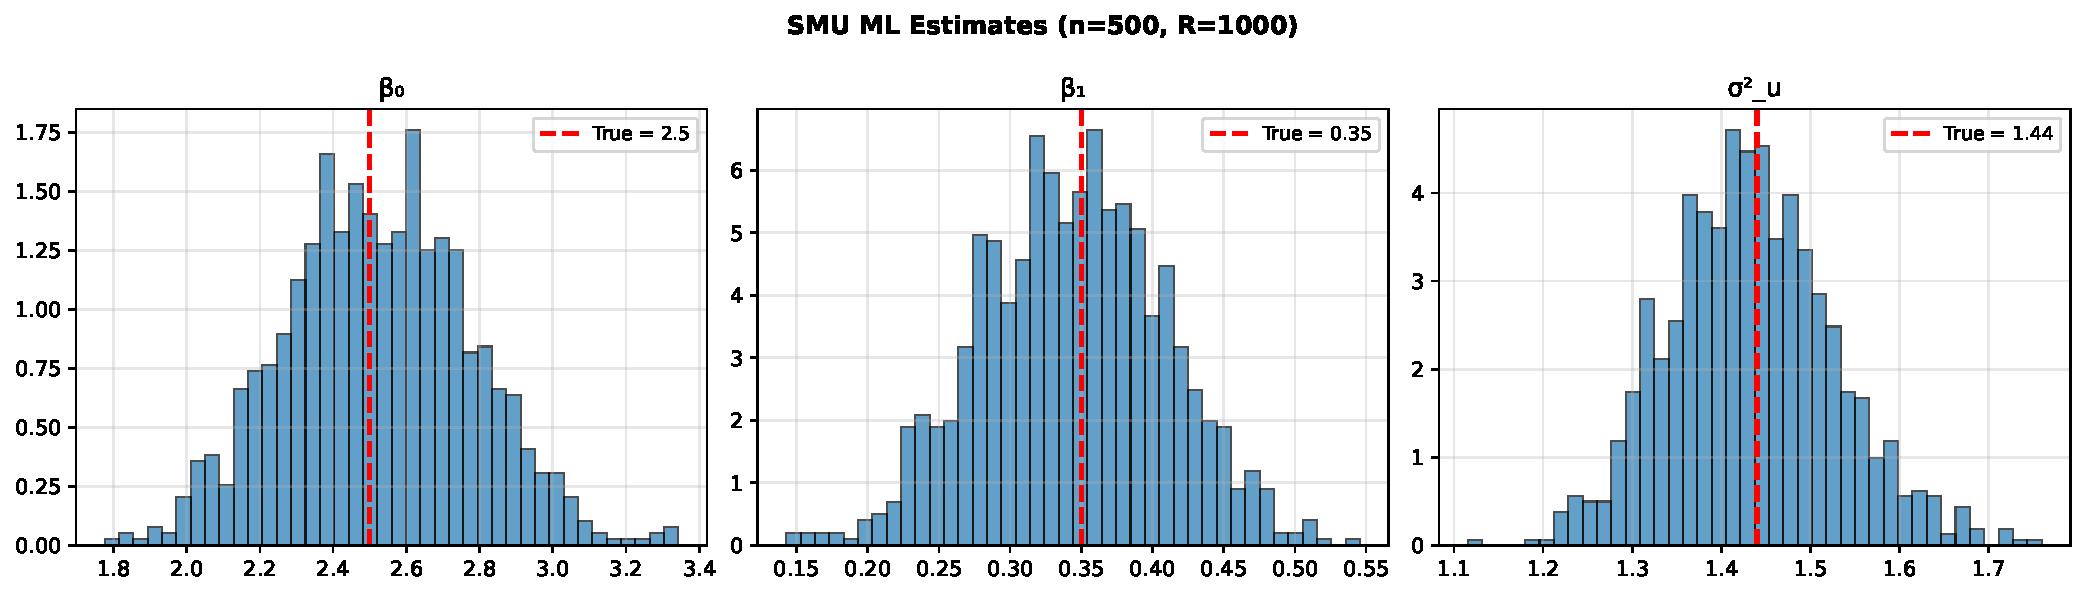
\includegraphics[width=\textwidth]{figures/mc_hist_smu_ml.pdf}
    \caption[Histograms of SMU ML estimates]{The figure shows histograms of $R = 1{,}000$ replications of SMU ML estimates. The true parameter values are marked by dashed red lines. We note that all three distributions are centred around the true value, showing approximate unbiasedness of the estimators.}
    \label{fig:mc_hist_smu_ml}
\end{figure}

\subsection{WB Equation}
\label{sec:mc:ml_wb}
Moving on to the WB equation, we apply Algorithm~\ref{alg:wb_ml}. Results are reported in Table~\ref{tab:mc_ml_results}, and histograms in Figure~\ref{fig:mc_hist_wb_ml}. The results are similar to those for the SMU equation: we have low bias, correspondence between standard errors, and good confidence interval coverage for all parameters, with the intercept $\gamma_0$ again showing higher bias and standard deviation. This is due to the same mechanism as before (see detailed explanation above for the SMU equation): the mean of the reduced form of $\vect{y}$ depends on $\gamma_0(1 - \gamma_3)^{-1}$, making the intercept partially confounded with the peer effect. Both the parameter $\gamma_2$ for the CoMO effect and $\gamma_3$ for the influence of peer WB are correctly estimated.

\begin{table}[htbp]
\centering
\caption[Monte Carlo results for WB ML estimator]{Monte Carlo results for WB ML estimator ($n = 500$, $R = 1{,}000$).}
\label{tab:mc_ml_results}
\begin{tabular}{lcccccc}
\toprule
Parameter & True & Mean Est. & Bias & Std(Est.) & Mean SE & Coverage \\
\midrule
$\gamma_0$ & 7.0 & 7.0306 & 0.0306 & 0.5050 & 0.5074 & 0.945 \\
$\gamma_1$ & $-0.5$ & $-0.4988$ & 0.0012 & 0.0538 & 0.0548 & 0.963 \\
$\gamma_2$ & $-0.8$ & $-0.7959$ & 0.0041 & 0.0938 & 0.0947 & 0.948 \\
$\gamma_3$ & 0.25 & 0.2442 & $-0.0058$ & 0.0623 & 0.0622 & 0.944 \\
$\sigma_\varepsilon^2$ & 1.00 & 0.9939 & $-0.0061$ & 0.0617 & 0.0632 & 0.956 \\
\bottomrule
\end{tabular}
\end{table}

\begin{figure}[htbp]
    \centering
    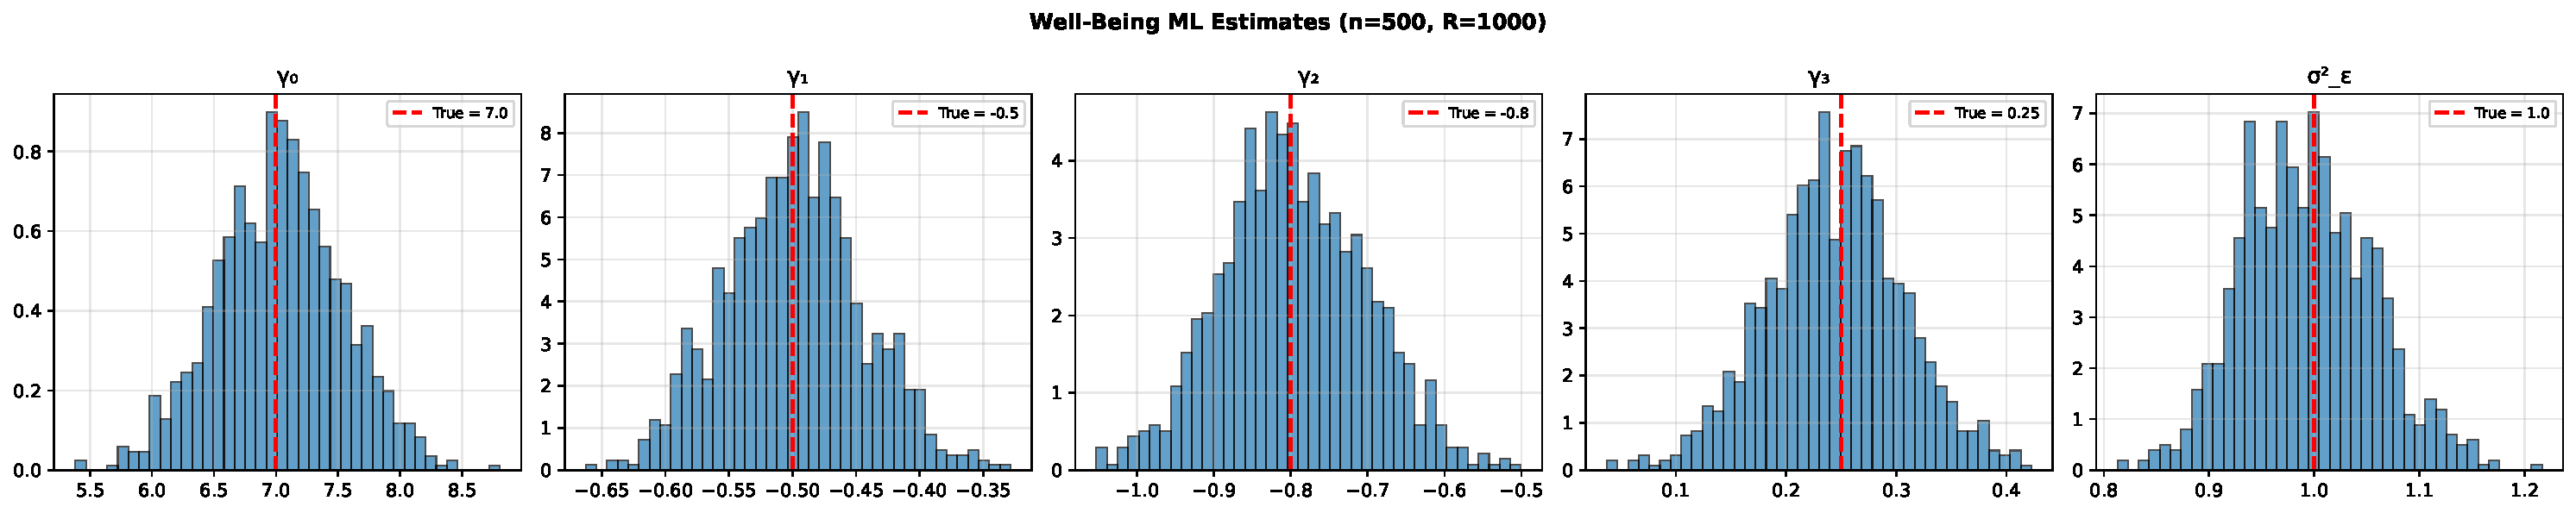
\includegraphics[width=\textwidth]{figures/mc_hist_wb_ml.pdf}
    \caption[Histograms of WB ML estimates]{Histograms of WB ML estimates across $R = 1{,}000$ replications. True parameter values shown as dashed red lines.}
    \label{fig:mc_hist_wb_ml}
\end{figure}

\subsection{Asymptotic Normality}
\label{sec:mc:normality}
We now validate the asymptotic normality of the ML estimators. Following the asymptotic theory of Section~\ref{sec:est:regularity} (see also Theorem~\ref{thm:mle_asymptotic}), we expect the standardised $z$-scores~\eqref{eq:mc_zscore_def} to be approximately $\N(0, 1)$-distributed.

For the WB equation, we plot histograms together with $\N(0, 1)$ overlays in Figure~\ref{fig:mc_zscore_hist}, and provide quantile-quantile plots in Figure~\ref{fig:mc_qq_ml}. Both show a close fit to the normal approximation for all estimated parameters. The empirical distributions follow the $\N(0, 1)$ reference closely, and the points in the Q-Q plots lie tightly along the diagonal with no evidence of heavy tails. These results confirm that the asymptotic approximation is adequate when $n = 500$.

\begin{figure}[htbp]
    \centering
    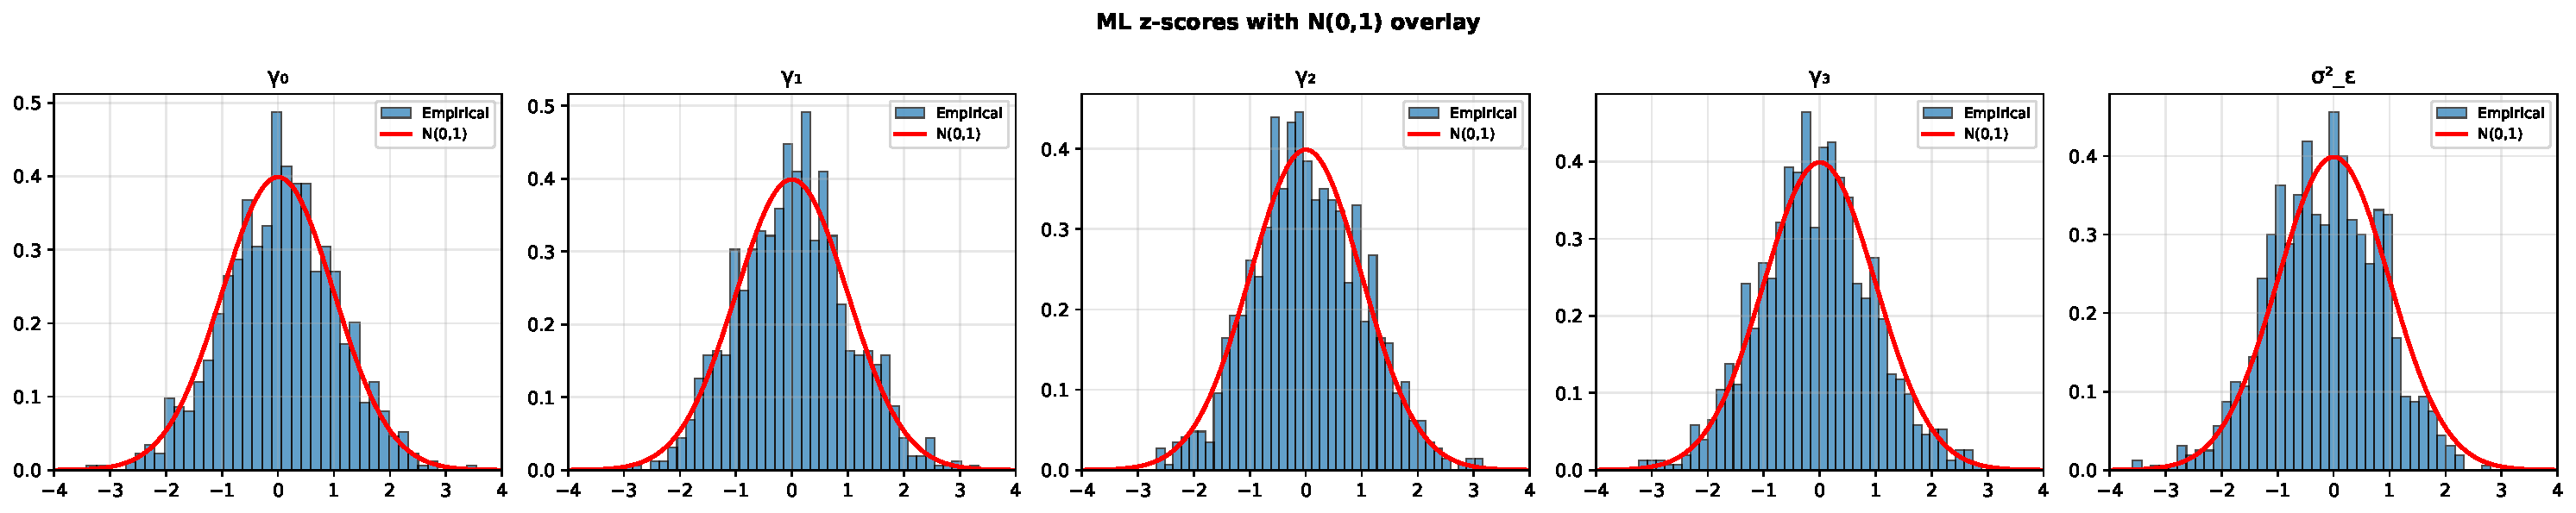
\includegraphics[width=\textwidth]{figures/mc_zscore_hist.pdf}
    \caption[Histograms of WB ML $z$-scores with $\N(0,1)$ overlays]{Histograms of ML $z$-scores with $\N(0,1)$ overlays (red curves) for each WB parameter.}
    \label{fig:mc_zscore_hist}
\end{figure}

\begin{figure}[htbp]
    \centering
    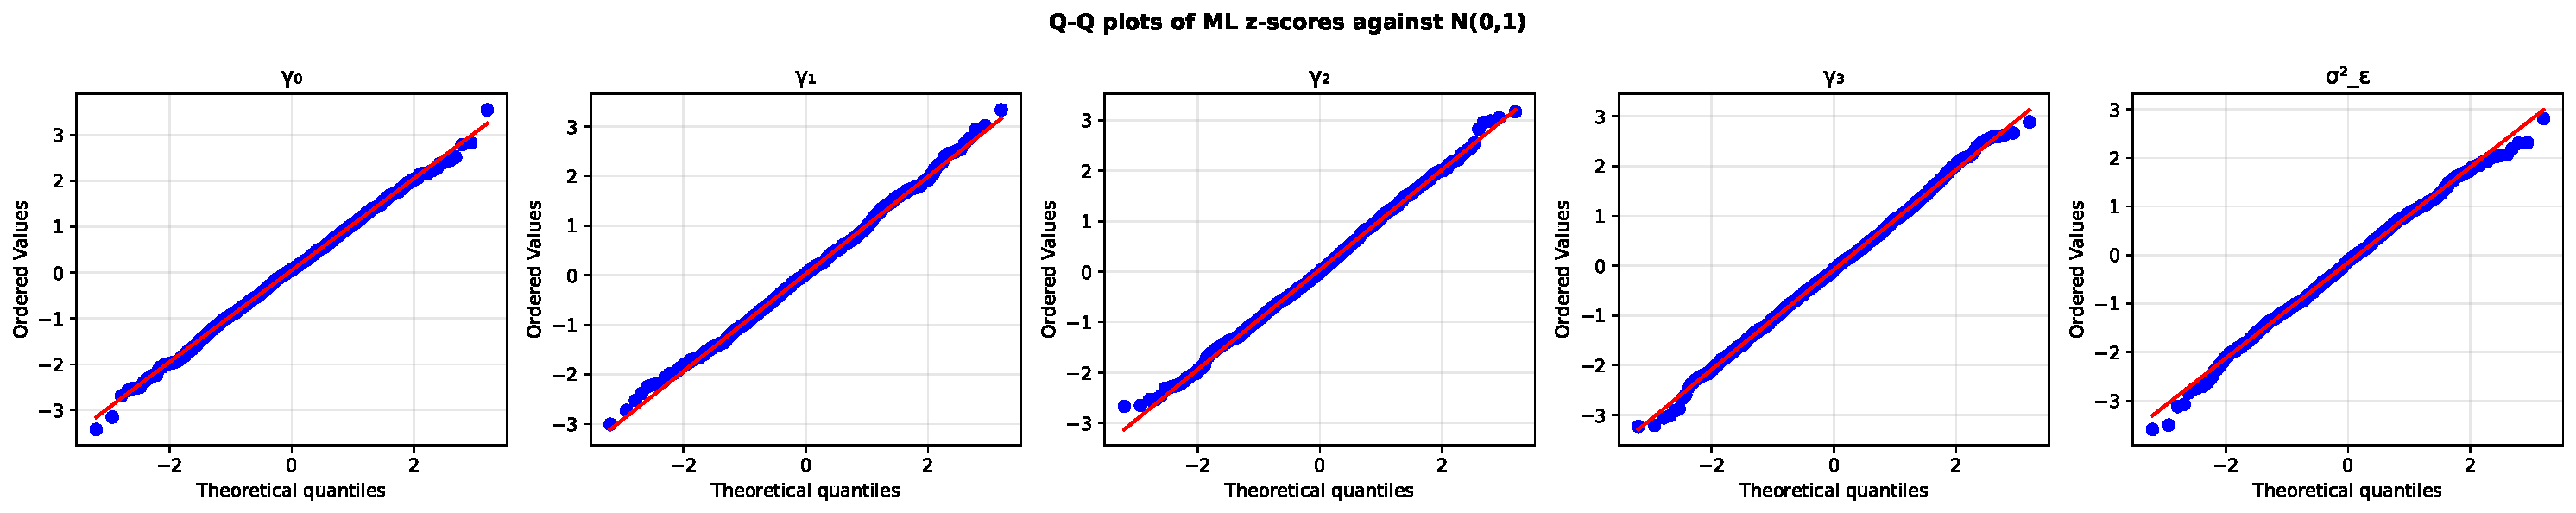
\includegraphics[width=\textwidth]{figures/mc_qq_ml.pdf}
    \caption[Q-Q plots of WB ML $z$-scores against $\N(0,1)$ quantiles]{Q-Q plots of empirical ML $z$-scores against the theoretical $\N(0,1)$ quantiles.}
    \label{fig:mc_qq_ml}
\end{figure}

We also provide an overview of summary statistics for the ML $z$-scores in Table~\ref{tab:mc_zscores_wb}. Here, all means are within $0.16$ of zero, and standard deviations within $0.02$ of $1$. This shows close correspondence with the theoretical mean of $0$ and standard deviation of $1$, respectively. The slightly larger discrepancy in the $\sigma_\varepsilon^2$ $z$-score mean (and similarly the $\sigma_u^2$ mean in Table~\ref{tab:mc_zscores_smu}) is consistent with general finite-sample downward bias of variance estimators for MLE \parencite[p.~331]{Casella2002}. The skewness and kurtosis are also negligible.

The ML $z$-scores for the SMU equation show similar results. For brevity, we omit the overlay and Q-Q plots, instead only reporting the summary statistics in Table~\ref{tab:mc_zscores_smu}. These also show a good correspondence with the expected theoretical values.

\begin{table}[htbp]
\centering
\caption[Summary statistics of WB ML $z$-scores]{Summary statistics of WB ML $z$-scores ($n = 500$, $R = 1{,}000$).}
\label{tab:mc_zscores_wb}
\begin{tabular}{lcccc}
\toprule
Parameter & Mean($z$) & Std($z$) & Skewness & Kurtosis \\
\midrule
$\gamma_0$ & 0.050 & 0.999 & $-0.070$ & 0.008 \\
$\gamma_1$ & 0.028 & 0.980 & 0.113 & $-0.098$ \\
$\gamma_2$ & 0.041 & 0.988 & 0.103 & $-0.139$ \\
$\gamma_3$ & $-0.079$ & 1.001 & 0.014 & 0.070 \\
$\sigma_\varepsilon^2$ & $-0.158$ & 0.983 & $-0.132$ & $-0.072$ \\
\bottomrule
\end{tabular}
\end{table}

\begin{table}[htbp]
\centering
\caption[Summary statistics of SMU ML $z$-scores]{Summary statistics of SMU ML $z$-scores ($n = 500$, $R = 1{,}000$).}
\label{tab:mc_zscores_smu}
\begin{tabular}{lcccc}
\toprule
Parameter & Mean($z$) & Std($z$) & Skewness & Kurtosis \\
\midrule
$\beta_0$ & 0.068 & 1.027 & $-0.059$ & $-0.123$ \\
$\beta_1$ & $-0.074$ & 1.028 & 0.095 & $-0.108$ \\
$\sigma_u^2$ & $-0.138$ & 1.023 & $-0.156$ & 0.192 \\
\bottomrule
\end{tabular}
\end{table}

%% Section 6.3: 2SLS Estimator Validation
\section{2SLS Estimator Validation}
\label{sec:mc:2sls}
In this section, we perform the Monte Carlo simulations validating the 2SLS estimator for the WB equation. A caveat on instrument strength should be kept in mind while reading this section. At the base $p = 0.01$ network density level, instrument strength is only moderate, with about $76\%$ of replications exceeding the \textcite[p.~557]{Staiger1997} threshold of $F = 10$. For the full diagnostics, see Section~\ref{sec:mc:first_stage}.

\subsection{Validation of the WB Equation}
\label{sec:mc:2sls_wb}
We now perform a Monte Carlo simulation to validate the 2SLS estimator of Section~\ref{sec:est:wb_2sls} for the WB equation, similar to that used for the ML estimator. We use the same instrument set as in~\eqref{eq:instrument_set}, $\mat{Z} = [\vect{1}, \vect{s}, \vect{c}, \mat{G}\vect{c}, \mat{G}^2\vect{s}, \mat{G}^2\vect{c}]$. We report the results in Table~\ref{tab:mc_2sls_results}, and display histograms of the estimates in Figure~\ref{fig:mc_hist_2sls}. Our results support the estimation strategy. Low bias, correspondence between empirical and HC1 standard errors, and coverage close to $95\%$ all indicate that the estimator is approximately unbiased and well-calibrated. We note that the coverage being consistently slightly above $95\%$ is in line with conservative standard errors when instrument strength is moderate (see Section~\ref{sec:mc:first_stage}).

We do not have a direct estimate of $\sigma_\varepsilon^2$ from the 2SLS estimator. If needed, we could obtain this indirectly from the residual variance. As we want to verify the 2SLS method specifically in this section, our results do not include this parameter.

\begin{table}[htbp]
\centering
\caption[Monte Carlo results for WB 2SLS estimator]{Monte Carlo results for WB 2SLS estimator ($n = 500$, $R = 1{,}000$).}
\label{tab:mc_2sls_results}
\begin{tabular}{lcccccc}
\toprule
Parameter & True & Mean Est. & Bias & Std(Est.) & Mean SE & Coverage \\
\midrule
$\gamma_0$ & 7.0 & 6.9227 & $-0.0773$ & 2.2312 & 2.2503 & 0.968 \\
$\gamma_1$ & $-0.5$ & $-0.4921$ & 0.0079 & 0.0792 & 0.0828 & 0.964 \\
$\gamma_2$ & $-0.8$ & $-0.7844$ & 0.0156 & 0.1125 & 0.1167 & 0.965 \\
$\gamma_3$ & 0.25 & 0.2564 & 0.0064 & 0.3138 & 0.3141 & 0.968 \\
\bottomrule
\end{tabular}
\end{table}

\begin{figure}[htbp]
    \centering
    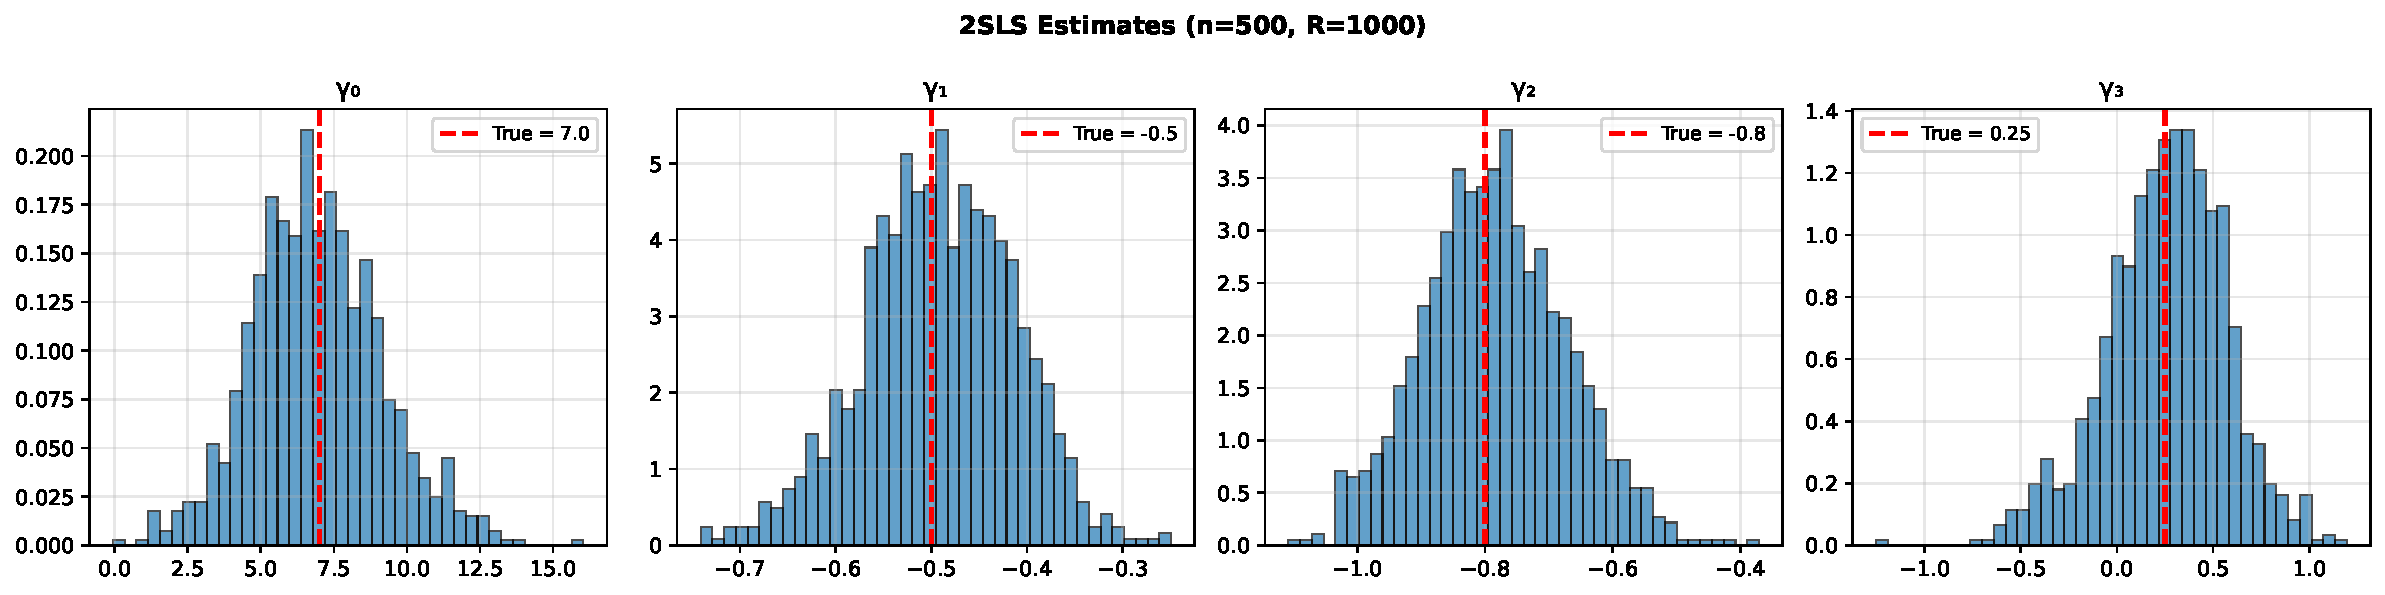
\includegraphics[width=\textwidth]{figures/mc_hist_2sls.pdf}
    \caption[Histograms of WB 2SLS estimates]{The figure shows histograms of 2SLS estimates from $R = 1{,}000$ Monte Carlo replications. We mark the true parameter values with dashed red lines.}
    \label{fig:mc_hist_2sls}
\end{figure}

\subsection{First-Stage Diagnostics}
\label{sec:mc:first_stage}
We now move on to tests and diagnostics of the 2SLS estimators (see Section~\ref{sec:est:diagnostics}), starting with the first-stage $F$-statistic.

This statistic tests the first stage of the 2SLS regression by checking whether the regression of $\mat{G}\vect{y}$ on $\mat{Z}$ has sufficient explanatory power. If it does not, we cannot expect 2SLS inference to be reliable. In our main Monte Carlo simulation for the 2SLS estimator, we thus also calculate the $F$-statistic for each of the $R = 1{,}000$ replications. A plot of the distribution of first-stage $F$-statistics is shown in Figure~\ref{fig:mc_fstat_hist}.

\begin{figure}[htbp]
    \centering
    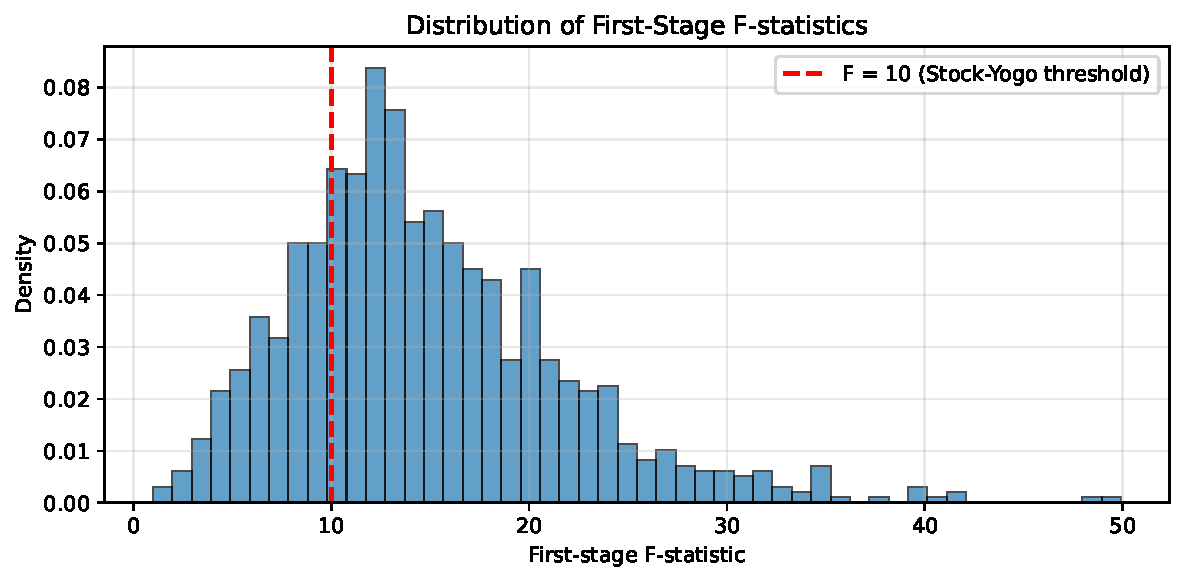
\includegraphics[width=0.8\textwidth]{figures/mc_fstat_hist.pdf}
    \caption[Distribution of first-stage $F$-statistics]{The figure plots the distribution of first-stage $F$-statistics for the $R = 1{,}000$ Monte Carlo replications. We mark the \textcite{Staiger1997} threshold of $F = 10$ with a dashed red line. Around $76\%$ of replications are above this threshold.}
    \label{fig:mc_fstat_hist}
\end{figure}

When interpreting these values, we follow the rule of thumb of \textcite{Staiger1997} and consider instruments that have $F < 10$ to be weak (for more details, see also the formal critical values of \textcite[Table~1]{StockYogo2005}). We report summary statistics including the fraction of replications with $F > 10$ in Table~\ref{tab:mc_fstat}.

\begin{table}[htbp]
\centering
\caption[First-stage $F$-statistic summary]{First-stage $F$-statistic summary ($n = 500$, $R = 1{,}000$).}
\label{tab:mc_fstat}
\begin{tabular}{lc}
\toprule
Statistic & Value \\
\midrule
Mean $F$ & 14.78 \\
Median $F$ & 13.55 \\
Fraction $F > 10$ & 0.759 \\
Fraction $F > 20$ & 0.202 \\
\bottomrule
\end{tabular}
\end{table}

Both the mean and median $F$-statistics of $14.78$ and $13.55$, respectively, are above the \textcite{Staiger1997} threshold of $10$. However, the fraction of $F$-statistics above $10$, at $75.9\%$, indicates that around $24\%$ of replications might have weak instruments. Based on this, we conclude that at $n = 500$ and $p = 0.01$, we have moderately strong instruments. In most replications, instruments are strong, and we obtain well-calibrated estimates in terms of bias and coverage. However, there are replications with weaker instruments, which might make 2SLS less efficient and thus the ML estimator preferable when the ML distributional requirements are met. This is also confirmed by the standard deviations, which are larger for the 2SLS estimates (Table~\ref{tab:mc_2sls_results}) than for the ML estimates (Table~\ref{tab:mc_ml_results}). The implication of these results is that researchers should take care to verify instrument strength before applying the 2SLS estimator.

\subsection{Overidentification and Hausman Tests}
\label{sec:mc:overid}
We now move on to the overidentification and Hausman tests (see Section~\ref{sec:est:diagnostics}). The results are calculated based on the same Monte Carlo simulation as before, with $n = 500$ and $R = 1{,}000$, and are reported in Table~\ref{tab:mc_diagnostics}.

As we have three excluded instruments and one endogenous regressor, our model is overidentified, and we can apply the Sargan--Hansen $J$-test. When all excluded instruments are valid, we have that $J \sim \chi^2_2$, and test rejection at the $5\%$ level should happen in approximately $5\%$ of replications. From Table~\ref{tab:mc_diagnostics}, we see that our Monte Carlo rejection rate is $4\%$, slightly below the expected value. The deviation is modest, about $1.5$ standard errors below the expected value when $R = 1{,}000$, and could thus reflect sampling variability. However, it might also indicate a mild effect from weak instruments in some of the replications, which would be in line with the observed first-stage $F$-statistics discussed above.

The Hausman test compares OLS and 2SLS estimates. Our DGP includes the endogenous $\mat{G}\vect{y}$ by construction, which means we expect a rejection rate higher than the nominal $5\%$ level, as the Hausman test should indicate the presence of endogeneity. However, the results reported in Table~\ref{tab:mc_diagnostics} show a Hausman rejection rate of $4.8\%$, close to the size expected under no endogeneity. With the other test results in mind, this result is not very surprising. The Hausman test does not have much power when the efficiency gap between OLS and 2SLS is high \parencite[p.~1258]{Hausman1978}. In our case, without very strong instruments, 2SLS is relatively imprecise, which makes the Hausman test statistic too noisy to separate the two estimators. However, as we will see in Section~\ref{sec:mc:ols_bias}, there is substantial bias in the OLS estimate $\hat\gamma_3$. Thus, the endogeneity present in our model still matters, even if the Hausman test does not have the power to detect it.

\begin{table}[htbp]
\centering
\caption[Diagnostic test rejection rates]{Diagnostic test rejection rates ($n = 500$, $R = 1{,}000$).}
\label{tab:mc_diagnostics}
\begin{tabular}{lcc}
\toprule
Test & Rejection Rate & Expected \\
\midrule
Sargan--Hansen $J$-test (H$_0$: instruments valid) & 0.040 & $\approx 0.05$ \\
Hausman test (H$_0$: no endogeneity) & 0.048 & $\gg 0.05$ \\
\bottomrule
\end{tabular}
\end{table}

\begin{remark}[Hausman Test Edge Case]
We include a reminder of the potential for the Hausman test statistic to be undefined in some cases due to the possibility of the difference $\widehat{\Var}(\hat{\gamma}_{\text{2SLS}}) - \widehat{\Var}(\hat{\gamma}_{\text{OLS}})$ in the denominator being negative in finite samples. Usually this should not occur, as 2SLS should have larger variance, but since the estimates are noisy, this might sometimes happen nonetheless. For our Monte Carlo run, this is not relevant, as it occurred in none of the $R = 1{,}000$ replications.
\end{remark}

\subsection{OLS Bias}
\label{sec:mc:ols_bias}
We end this section with a comparison to the OLS estimator. This estimator ignores the endogeneity of $\mat{G}\vect{y}$, which makes it biased compared to our ML and 2SLS estimators. The results for the (endogenous) $\gamma_3$ parameter are displayed in Table~\ref{tab:mc_ols_bias}. They show a much higher bias for OLS compared to the other two estimators. This is due to the simultaneity and network structure of our setup, which lead to a correlation between higher $\mat{G}\vect{y}$ and higher $\varepsilon_i$. OLS ends up with an inflated estimate of the peer effect, while our ML and 2SLS estimators correctly handle the endogenous regressor.

\begin{table}[htbp]
\centering
\caption[OLS, ML, and 2SLS bias comparison for $\gamma_3$]{OLS, ML, and 2SLS bias comparison for $\gamma_3$ ($n = 500$, $R = 1{,}000$).}
\label{tab:mc_ols_bias}
\begin{tabular}{lccc}
\toprule
Method & Mean $\hat\gamma_3$ & Bias & RMSE \\
\midrule
OLS & 0.4050 & 0.1550 & 0.1852 \\
ML & 0.2442 & $-0.0058$ & 0.0625 \\
2SLS & 0.2564 & 0.0064 & 0.3139 \\
\bottomrule
\end{tabular}
\end{table}

%% Section 6.4: Comparison of ML and 2SLS
\section{Comparison of ML and 2SLS}
\label{sec:mc:comparison}
We have validated both the ML and 2SLS estimators. Now we will compare their performance in finite samples for the WB equation. This will give us insight into when it is preferable to use one or the other. This section builds on the theoretical comparison of Section~\ref{sec:est:comparison}.

We begin with a comparison of the bias and efficiency of the estimators. As we are working under an assumption of normality, we expect the ML estimator to outperform the 2SLS estimator. This is exactly what we find. In Table~\ref{tab:mc_comparison}, we report the bias and RMSE comparison of the two methods, along with a measure of relative efficiency, defined as $\text{RMSE}_{\text{2SLS}} / \text{RMSE}_{\text{ML}}$. Under normality, the relative efficiency should be $\geq 1$ for all parameters, as the ML estimator is more efficient than 2SLS, with magnitude depending on instrument strength. Our results show a lower bias for the ML estimator across the board, and relative efficiencies ranging from around $1.2$ to $5.0$. The highest relative efficiencies are for $\gamma_0$ ($4.41$) and $\gamma_3$ ($5.02$). The latter corresponds well with the previous test result showing that the instruments are only moderately strong. For $\gamma_0$, the efficiency gap can be explained by the intercept identification issue discussed in Section~\ref{sec:mc:ml_wb}.

\begin{table}[htbp]
\centering
\caption[ML vs.\ 2SLS comparison for the WB equation]{ML vs.\ 2SLS comparison for the WB equation ($n = 500$, $R = 1{,}000$).}
\label{tab:mc_comparison}
\begin{tabular}{lccccc}
\toprule
 & \multicolumn{2}{c}{Bias} & \multicolumn{2}{c}{RMSE} & Relative \\
\cmidrule(lr){2-3} \cmidrule(lr){4-5}
Parameter & ML & 2SLS & ML & 2SLS & Efficiency \\
\midrule
$\gamma_0$ & 0.0306 & $-0.0773$ & 0.5059 & 2.2325 & 4.41 \\
$\gamma_1$ & 0.0012 & 0.0079 & 0.0539 & 0.0796 & 1.48 \\
$\gamma_2$ & 0.0041 & 0.0156 & 0.0939 & 0.1136 & 1.21 \\
$\gamma_3$ & $-0.0058$ & 0.0064 & 0.0625 & 0.3139 & 5.02 \\
\bottomrule
\end{tabular}
\end{table}

We further compare ML and 2SLS through scatter plots of the estimates in Figure~\ref{fig:mc_ml_vs_2sls_scatter}. Here, agreement corresponds to a clustering of points around the identity line, which would indicate that the estimators recover the same underlying parameters. We see a relatively good correspondence between the estimators for the $\gamma_1$ and $\gamma_2$ parameters, with a difference for the $\gamma_3$ parameter. This is due to the higher efficiency of the ML estimator for this parameter, making the ML points cluster more tightly around the true value.

\begin{figure}[htbp]
    \centering
    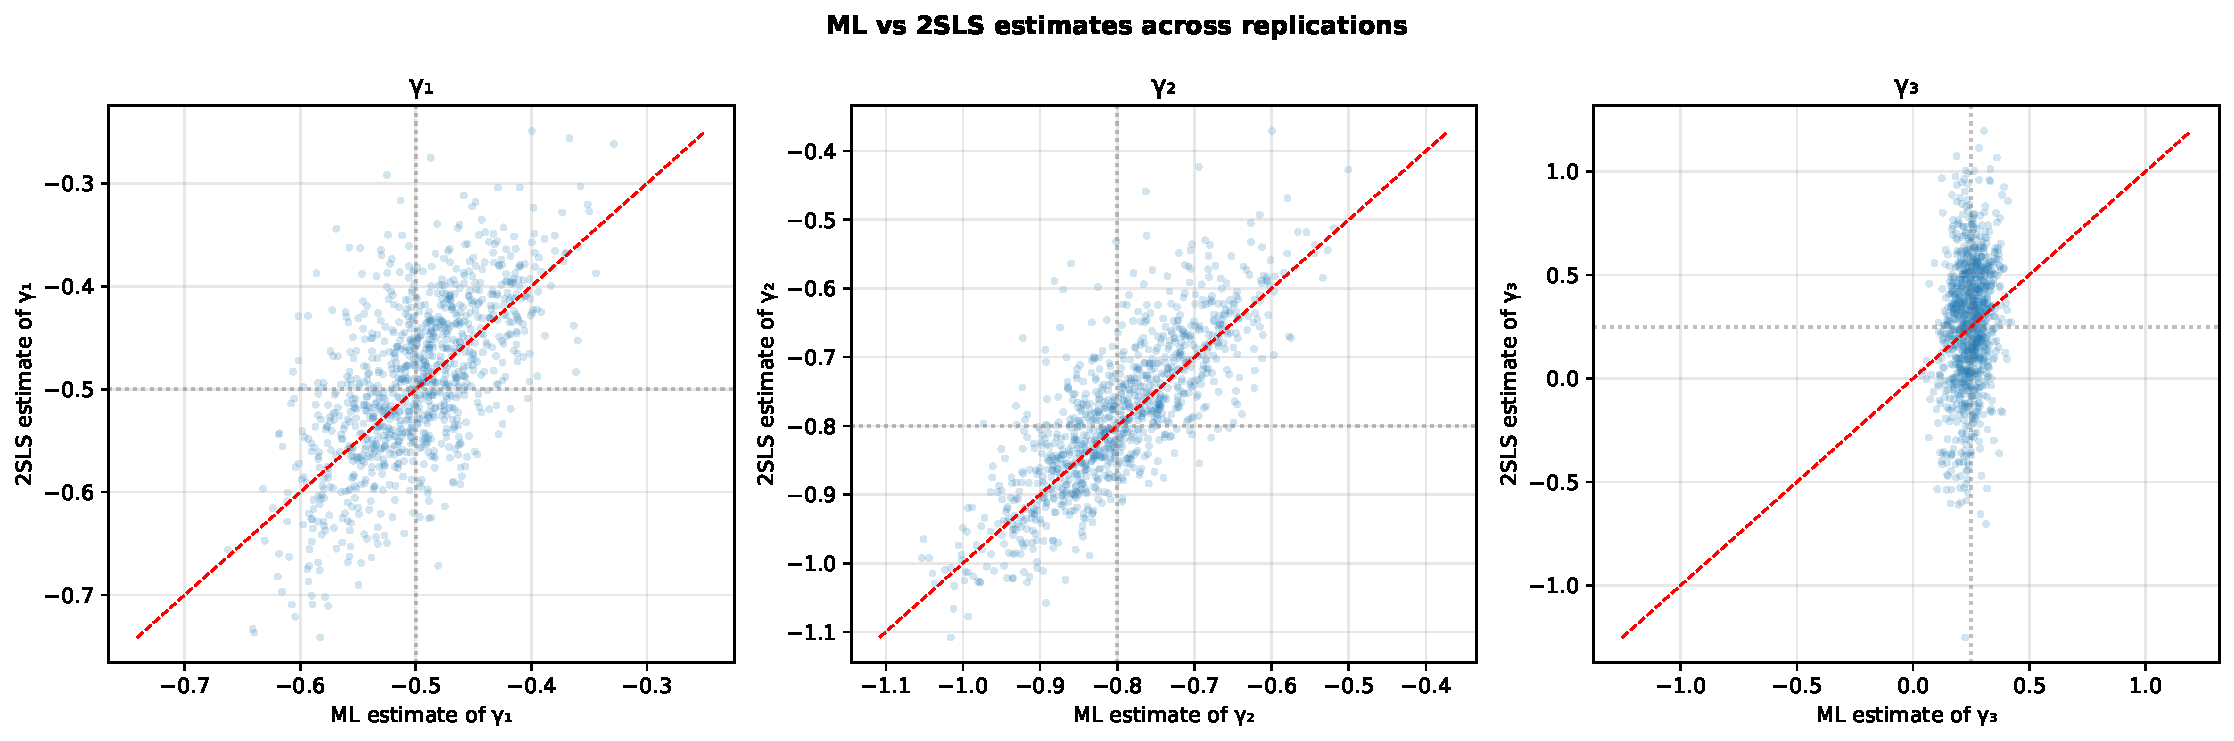
\includegraphics[width=\textwidth]{figures/mc_ml_vs_2sls_scatter.pdf}
    \caption[Scatter plots of ML vs.\ 2SLS estimates]{Scatter plots of ML vs.\ 2SLS estimates for $\gamma_1$, $\gamma_2$, and $\gamma_3$ across the Monte Carlo replications. The dashed red line is the identity line. We note a higher variance for the 2SLS estimates, especially for $\gamma_3$.}
    \label{fig:mc_ml_vs_2sls_scatter}
\end{figure}

%% Section 6.5: Wald Test Calibration
\section{Wald Test Calibration}
\label{sec:mc:wald}
In Section~\ref{sec:est:testing}, we developed a Wald test for the CoMO coefficient $\gamma_2$, and a joint Wald test for the network-term coefficients $\gamma_2$ and $\gamma_3$. This section validates these. The two null hypotheses are
\begin{align}
    H_0^{(a)}&: \gamma_2 = 0 \quad \text{(no CoMO effect, single Wald test)}, \\
    H_0^{(b)}&: \gamma_2 = \gamma_3 = 0 \quad \text{(no network effects, joint Wald test)}.
\end{align}

We evaluate the empirical sizes of the tests: the number of times they reject under the null hypotheses, for both the ML and the 2SLS covariance estimators. The Hessian-based standard errors of~\eqref{eq:se_formula} are used for the ML approach, where the analytical observed information matrix of Section~\ref{sec:est:wb_hessian} is inverted, and the $(\gamma_2, \gamma_3)$ block is extracted. The corresponding block of the HC1-robust sandwich matrix from~\eqref{eq:robust_se} is used for 2SLS\@. Using these, we can compute the test for $\gamma_2$ as $t = \hat\gamma_2 / \widehat{\text{SE}}(\hat\gamma_2)$ and for $\gamma_2$ and $\gamma_3$ as $W = \hat{\gammavec}_R^\top [\mat{R}\,\widehat{\Var}(\hat{\thetavec}_y)\,\mat{R}^\top]^{-1} \hat{\gammavec}_R$ (see Section~\ref{sec:est:testing}). These statistics are asymptotically standard-normal and $\chi^2_2$ distributed, respectively.

The Monte Carlo simulations are run with $n = 500$, $p = 0.01$, $R = 1{,}000$, and network generation as in Section~\ref{sec:mc:procedure}. The null DGP uses the same parameters as in Table~\ref{tab:mc_true_params} except that we set $\gamma_2 = \gamma_3 = 0$. We use this same DGP for both tests, as it satisfies both null hypotheses. We do not verify the size of the single-hypothesis test when $\gamma_3 \neq 0$ here. We compare the sizes to the nominal level of $\alpha = 0.05$. The rejection rates are reported in Table~\ref{tab:mc_wald}. We also show the empirical cumulative distribution functions (CDFs) of the joint Wald $p$-values in Figure~\ref{fig:mc_wald_pvalues}. Under correct calibration, these should lie on 45-degree lines in the plots.

\begin{table}[htbp]
\centering
\caption[Wald test size]{Wald test size ($n = 500$, $R = 1{,}000$, $\alpha = 0.05$). Size is the rejection rate under the null DGP ($\gamma_2 = \gamma_3 = 0$).}
\label{tab:mc_wald}
\begin{tabular}{llc}
\toprule
Estimator & Test (null hypothesis) & Size \\
\midrule
ML   & Single $(H_0: \gamma_2 = 0)$              & 0.050 \\
ML   & Joint  $(H_0: \gamma_2 = \gamma_3 = 0)$   & 0.045 \\
2SLS & Single $(H_0: \gamma_2 = 0)$              & 0.041 \\
2SLS & Joint  $(H_0: \gamma_2 = \gamma_3 = 0)$   & 0.038 \\
\bottomrule
\end{tabular}
\end{table}

\begin{figure}[htbp]
    \centering
    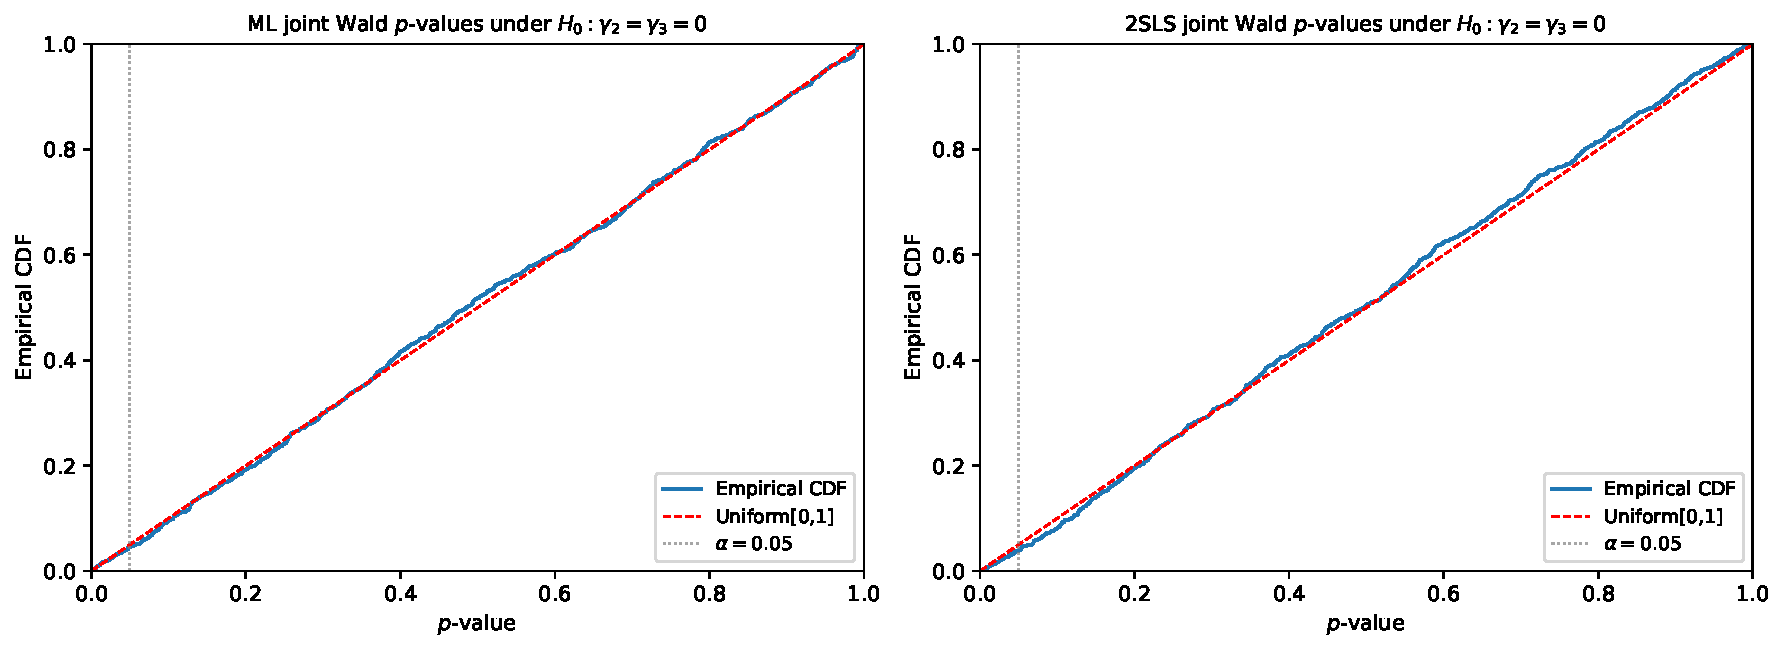
\includegraphics[width=\textwidth]{figures/mc_wald_pvalues.pdf}
    \caption[Empirical CDFs of joint Wald $p$-values under the null]{The plots show empirical CDFs of joint Wald $p$-values under the null DGP, with covariance estimators for ML in the left panel, and 2SLS in the right panel. We mark the theoretical $\text{Uniform}[0, 1]$ CDF with a red dashed line. The dotted vertical line shows the nominal level $\alpha = 0.05$ used for reporting the values in Table~\ref{tab:mc_wald}.}
    \label{fig:mc_wald_pvalues}
\end{figure}

The results show a good calibration under the null across the four tests. For $R = 1{,}000$ replications, the Monte Carlo standard error of a rejection rate near $0.05$ is $\sqrt{0.05 \times 0.95 / 1{,}000} \approx 0.007$. This gives the two-standard-error band of $0.036$ to $0.064$ around the nominal level. All sizes are within this band, with the ML rejection rates of $0.050$ and $0.045$ being very close to nominal, and the 2SLS rejection rates of $0.041$ and $0.038$ being slightly below it. The mild under-rejection of 2SLS might be explained by the HC1 standard errors being conservative (see Section~\ref{sec:mc:2sls}). The CDF plots of Figure~\ref{fig:mc_wald_pvalues} confirm the good calibration, with empirical CDFs close to the expected 45-degree lines. Together with the $z$-score analysis of Section~\ref{sec:mc:normality}, these results provide evidence that the asymptotic approximations of Section~\ref{sec:est:testing} hold when $n = 500$.

We do not include an empirical power study here, as at the current DGP the coefficients are large enough that single-point power is uninformative. A comparable power analysis for the nested Wald test in the simultaneous CoMO model is reported in Section~\ref{sec:simul:wald_test}.

%% Section 6.6: Effect of Network Density
\section{Effect of Network Density}
\label{sec:mc:density}
Differences in network density can affect the performance of estimators. Because of this, we include a section testing estimator robustness under varying network densities.

When network density changes, this also changes the number of connections per individual in the network. As $\mat{G}$ is row-normalised, this leads to neighbour averages being computed over a different number of neighbours, which in turn affects $\mat{G}\vect{y}$. With higher density, this term becomes more homogeneous, which can make instruments weaker and hence also degrade the performance of 2SLS estimators.

To investigate the effect of network density, we perform Monte Carlo simulations with varying levels of the connection probability $p$:
\begin{equation}
    p \in \{0.01, 0.02, 0.03, 0.05, 0.10\}
\end{equation}

We use $n = 500$ individuals, and thus get the expected degrees of approximately $5$, $10$, $15$, $25$, and $50$ for these networks. This creates examples ranging from a moderately sparse network to a relatively homogeneous one, allowing us to properly test our estimators. To reduce the computational burden, we lower the number of replications to $R = 500$ (from $R = 1{,}000$ previously). Otherwise, we keep the exact same DGP parameters as before (see Table~\ref{tab:mc_true_params}). We focus on the $\gamma_2$ and $\gamma_3$ parameters, as their identification depends most directly on the network structure. When changing $\mat{G}$ and the instruments derived from it, these are thus the most informative parameters to track. The remaining parameters are less sensitive to the network structure.

The main results are covered in Tables~\ref{tab:mc_density_g2} and~\ref{tab:mc_density_g3}, with corresponding plots in Figure~\ref{fig:mc_density_sensitivity}. We also report the mean first-stage $F$-statistic at each density, along with a verification that the Bramoull\'e identification condition (linear independence of $\mat{I}$, $\mat{G}$, and $\mat{G}^2$) holds, in Table~\ref{tab:mc_identification}.

\begin{table}[htbp]
\centering
\caption[Effect of network density on $\gamma_2$ estimation]{Effect of network density on $\gamma_2$ estimation ($n = 500$, $R = 500$).}
\label{tab:mc_density_g2}
\begin{tabular}{lccccccc}
\toprule
 & & \multicolumn{3}{c}{ML} & \multicolumn{3}{c}{2SLS} \\
\cmidrule(lr){3-5} \cmidrule(lr){6-8}
$p$ & Exp.\ Degree & Bias & RMSE & Coverage & Bias & RMSE & Coverage \\
\midrule
0.01 & 5 & $-0.0061$ & 0.0959 & 0.946 & 0.0060 & 0.1172 & 0.946 \\
0.02 & 10 & 0.0030 & 0.1053 & 0.948 & 0.0159 & 0.1228 & 0.946 \\
0.03 & 15 & 0.0052 & 0.1143 & 0.952 & 0.0194 & 0.1286 & 0.950 \\
0.05 & 25 & 0.0054 & 0.1210 & 0.944 & 0.0243 & 0.1345 & 0.962 \\
0.10 & 50 & 0.0052 & 0.1250 & 0.940 & 0.0166 & 0.1350 & 0.950 \\
\bottomrule
\end{tabular}
\end{table}

\begin{table}[htbp]
\centering
\caption[Effect of network density on $\gamma_3$ estimation]{Effect of network density on $\gamma_3$ estimation ($n = 500$, $R = 500$).}
\label{tab:mc_density_g3}
\begin{tabular}{lccccccc}
\toprule
 & & \multicolumn{3}{c}{ML} & \multicolumn{3}{c}{2SLS} \\
\cmidrule(lr){3-5} \cmidrule(lr){6-8}
$p$ & Exp.\ Degree & Bias & RMSE & Coverage & Bias & RMSE & Coverage \\
\midrule
0.01 & 5 & $-0.0087$ & 0.0633 & 0.942 & 0.0151 & 0.3047 & 0.962 \\
0.02 & 10 & $-0.0138$ & 0.0900 & 0.956 & 0.0134 & 0.6636 & 0.956 \\
0.03 & 15 & $-0.0229$ & 0.1101 & 0.972 & 0.0538 & 0.9472 & 0.964 \\
0.05 & 25 & $-0.0328$ & 0.1473 & 0.962 & 0.2460 & 1.6079 & 0.968 \\
0.10 & 50 & $-0.0637$ & 0.2157 & 0.938 & 0.4487 & 2.7588 & 0.980 \\
\bottomrule
\end{tabular}
\end{table}


\begin{table}[htbp]
\centering
\caption[Identification condition check and mean first-stage $F$-statistics]{Identification condition check and mean first-stage $F$-statistics ($n = 500$, $R = 500$).}
\label{tab:mc_identification}
\begin{tabular}{lcc}
\toprule
$p$ & Fraction with rank$[\mat{I}, \mat{G}, \mat{G}^2] = 3$ & Mean first-stage $F$ \\
\midrule
0.01 & 1.00 & 15.36 \\
0.02 & 1.00 & 8.95 \\
0.03 & 1.00 & 6.70 \\
0.05 & 1.00 & 4.91 \\
0.10 & 1.00 & 3.48 \\
\bottomrule
\end{tabular}
\end{table}

We first note the results of Table~\ref{tab:mc_identification}: the identification condition holds for all networks, and there is a decline in the mean first-stage $F$-statistic as network density grows. This is because the network becomes more homogeneous, leading instrument strength to decrease as less variation can be provided by the network structure. We now discuss the effect this has on our parameter estimates.

For the $\gamma_2$ parameter for the CoMO effect, both estimators perform well under the varying network densities. We find this in both Table~\ref{tab:mc_density_g2} and the plots of Figure~\ref{fig:mc_density_sensitivity} (top row). While we do observe a slightly degraded performance for denser networks in terms of an increase in RMSE (and, arguably, for the bias of the 2SLS estimator), the increase is not drastic. Both estimators have low bias and relatively good coverage at all simulated network densities.

The $\gamma_3$ parameter corresponding to the endogenous term tells a different story. As reported in Table~\ref{tab:mc_density_g3} and seen in Figure~\ref{fig:mc_density_sensitivity} (bottom row), the performance of the two estimators diverges as the density of the network grows. For the ML estimator, we observe a slight to moderate increase in both bias and RMSE as the density grows, with coverage staying near the nominal level. Thus, the performance degrades slightly with network density, but we still recover the parameter with low bias and standard deviation. The slight increase in ML bias for the $\gamma_3$ parameter might be caused by denser networks making $\mat{G}$ closer to a rank-one matrix, implying less curvature from the Jacobian term. This makes identifying $\gamma_3$ harder, as it becomes more confounded with the intercept. The 2SLS estimator, on the other hand, exhibits a sharp increase in both bias and RMSE as the network density increases. The coverage does stay close to nominal, but this might be due to increasingly wide confidence intervals, not actual performance, as the RMSE for $\hat\gamma_3$ increases by around an order of magnitude across the density range. The degradation of the 2SLS estimator is much more pronounced than for the ML estimator. This corresponds well with our previous reasoning: as the network density grows, the network becomes more homogeneous, weakening instrument strength. Homogeneous, well-connected networks do not provide the same network-based variation as sparse networks do, leading to a degradation of the 2SLS estimates. This is consistent with the observed decline in the $F$-statistics (Table~\ref{tab:mc_identification}).

\begin{figure}[htbp]
    \centering
    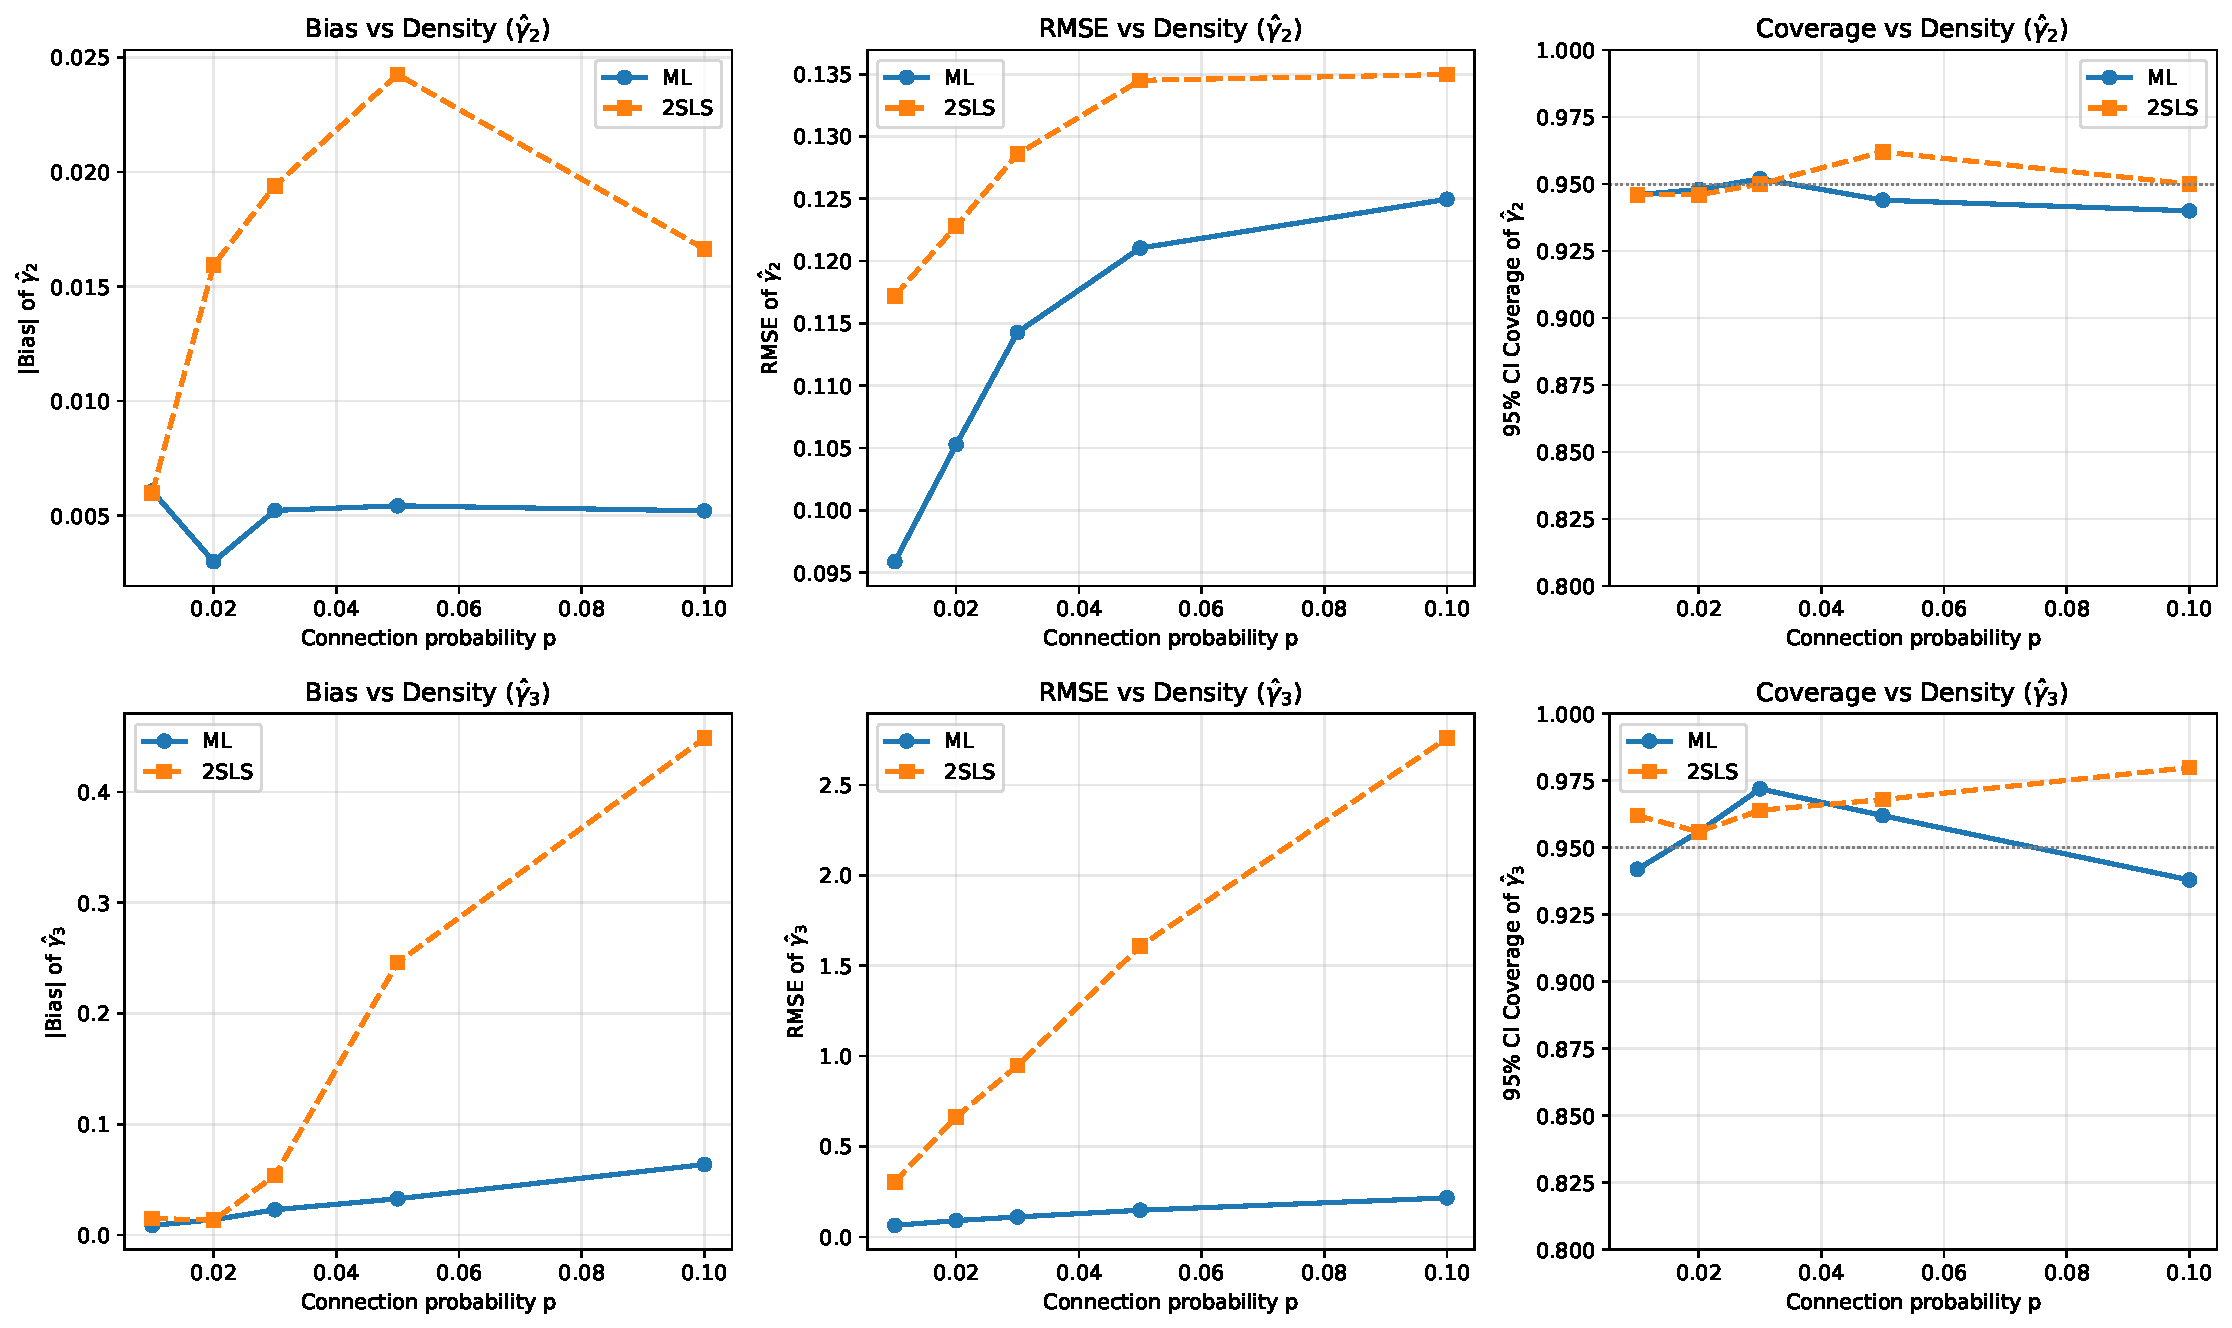
\includegraphics[width=\textwidth]{figures/mc_density_sensitivity.pdf}
    \caption[Effect of network density on bias, RMSE, and CI coverage]{We plot the effect of network density on absolute bias, RMSE, and $95\%$ CI coverage for $\hat\gamma_2$ (top row) and $\hat\gamma_3$ (bottom row). There is a stark difference between the ML and 2SLS performance for the endogenous $\gamma_3$ parameter.}
    \label{fig:mc_density_sensitivity}
\end{figure}

The results of our Monte Carlo simulations on network density show a divergence between the ML and 2SLS estimators. When networks are sparse, both estimators can be successfully applied. However, as density grows, the mean $F$-statistic quickly falls below the \textcite{Staiger1997} threshold of $10$. The 2SLS estimator degrades as weak-instrument issues arise. This leads to the following conclusion: for sparse networks, both the ML and 2SLS estimators can be applied, while in settings with denser networks, ML is preferred.

%% Section 6.7: Convergence as Sample Size Increases
\section{Convergence as Sample Size Increases}
\label{sec:mc:convergence}
Lastly, we perform simulations investigating the convergence as the sample size increases. We do this by increasing the size of the network while holding the expected degree constant. Keeping the degree constant allows us to isolate the effect of increased sample size, giving a complementary study to the density study of Section~\ref{sec:mc:density}. If the estimators work as expected, we should observe improved performance as $n$ grows.

To perform the simulations, we fix the expected degree at $10$ and simulate for the following sample sizes:
\begin{equation}
    n \in \{500, 750, 1{,}000, 1{,}500, 2{,}000\}
\end{equation}

To keep the expected degree fixed, we need to scale the connection probability $p$ as the network size increases. Setting $p = 10/(n-1)$, we get approximately $10$ as the expected number of connections per individual, along with $p \approx 0.020, 0.013, 0.010, 0.007, 0.005$ for the five sample sizes. Otherwise, we use the same DGP parameters as before (see Table~\ref{tab:mc_true_params}), and use $R = 500$ Monte Carlo replications.

As with the density study, we report results for the $\gamma_2$ and $\gamma_3$ parameters, since these are the most network-dependent and hence the most informative to investigate (see discussion in Section~\ref{sec:mc:density}). We report the results for $\gamma_2$ in Table~\ref{tab:mc_convergence_g2} and for $\gamma_3$ in Table~\ref{tab:mc_convergence_g3}, along with log-log plots of convergence for both in Figure~\ref{fig:mc_convergence}.

\begin{table}[htbp]
\centering
\caption[Convergence of ML and 2SLS estimators for $\gamma_2$]{Convergence of ML and 2SLS estimators for $\gamma_2$ (True = $-0.8$, $R = 500$).}
\label{tab:mc_convergence_g2}
\begin{tabular}{lccccccc}
\toprule
 & & \multicolumn{3}{c}{ML} & \multicolumn{3}{c}{2SLS} \\
\cmidrule(lr){3-5} \cmidrule(lr){6-8}
$n$ & $p$ & Bias & RMSE & Coverage & Bias & RMSE & Coverage \\
\midrule
500 & 0.0200 & $-0.0059$ & 0.1034 & 0.960 & 0.0084 & 0.1187 & 0.968 \\
750 & 0.0134 & 0.0008 & 0.0927 & 0.926 & 0.0124 & 0.1038 & 0.952 \\
1{,}000 & 0.0100 & 0.0007 & 0.0781 & 0.946 & 0.0072 & 0.0887 & 0.940 \\
1{,}500 & 0.0067 & 0.0012 & 0.0625 & 0.946 & 0.0072 & 0.0703 & 0.952 \\
2{,}000 & 0.0050 & 0.0032 & 0.0556 & 0.946 & 0.0055 & 0.0627 & 0.942 \\
\bottomrule
\end{tabular}
\end{table}

\begin{table}[htbp]
\centering
\caption[Convergence of ML and 2SLS estimators for $\gamma_3$]{Convergence of ML and 2SLS estimators for $\gamma_3$ (True = $0.25$, $R = 500$).}
\label{tab:mc_convergence_g3}
\begin{tabular}{lccccccc}
\toprule
 & & \multicolumn{3}{c}{ML} & \multicolumn{3}{c}{2SLS} \\
\cmidrule(lr){3-5} \cmidrule(lr){6-8}
$n$ & $p$ & Bias & RMSE & Coverage & Bias & RMSE & Coverage \\
\midrule
500 & 0.0200 & $-0.0096$ & 0.0920 & 0.956 & 0.0350 & 0.6827 & 0.962 \\
750 & 0.0134 & $-0.0167$ & 0.0783 & 0.946 & 0.0357 & 0.4970 & 0.954 \\
1{,}000 & 0.0100 & $-0.0106$ & 0.0668 & 0.946 & $-0.0084$ & 0.4552 & 0.966 \\
1{,}500 & 0.0067 & $-0.0027$ & 0.0556 & 0.942 & 0.0120 & 0.3549 & 0.954 \\
2{,}000 & 0.0050 & $-0.0003$ & 0.0458 & 0.950 & $-0.0051$ & 0.3082 & 0.968 \\
\bottomrule
\end{tabular}
\end{table}

\begin{figure}[htbp]
    \centering
    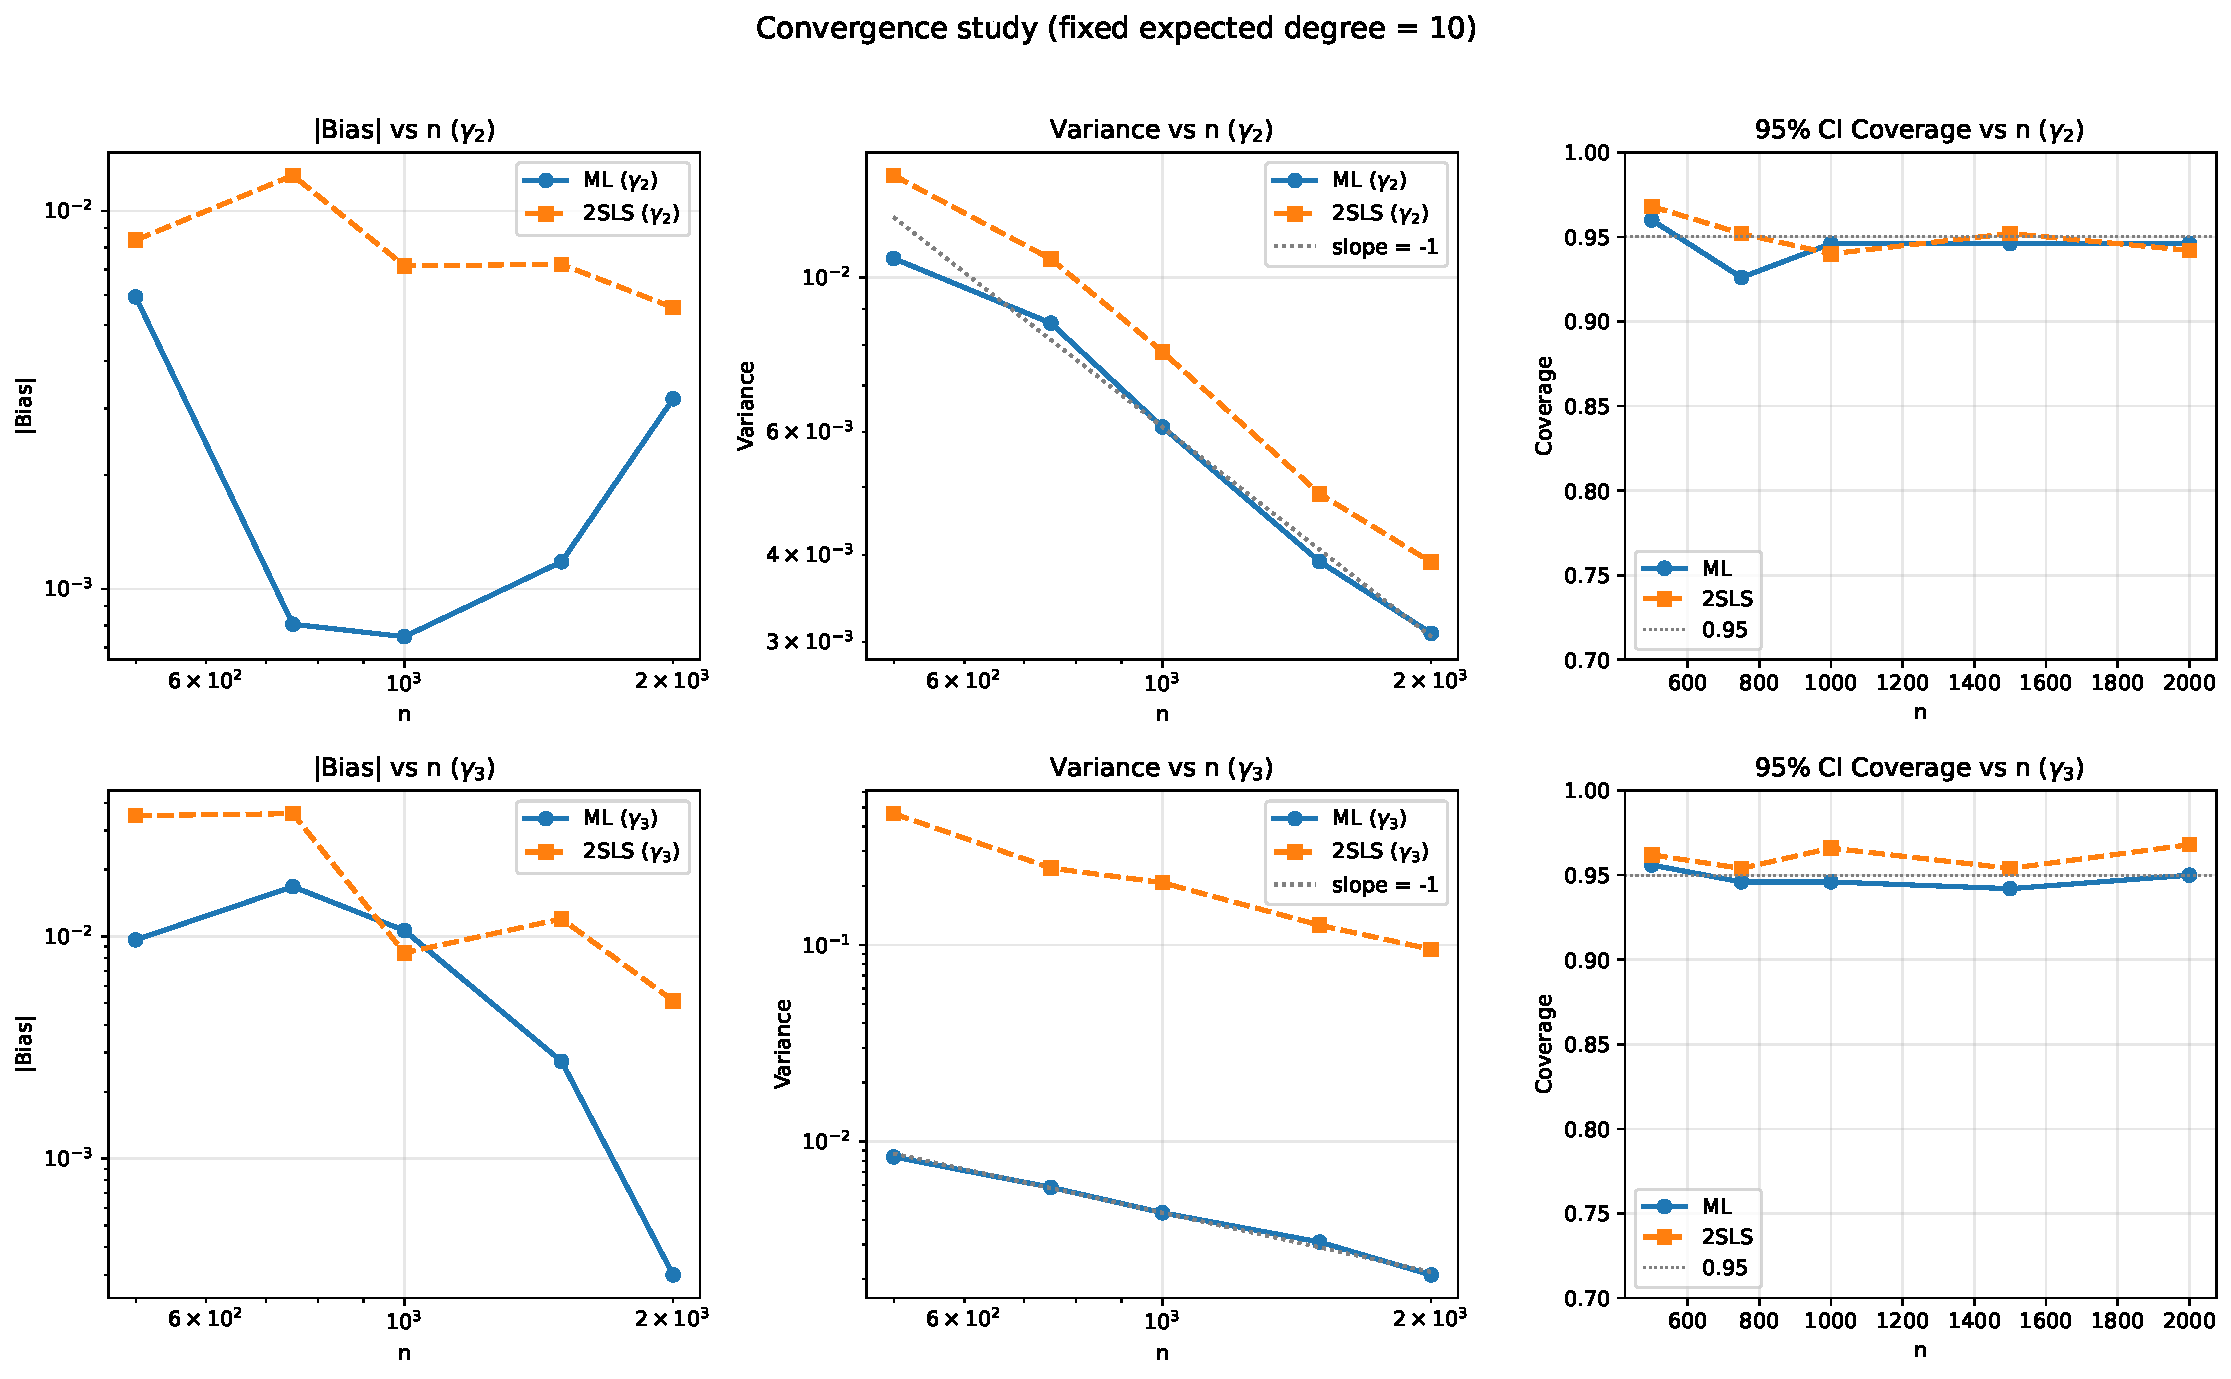
\includegraphics[width=\textwidth]{figures/mc_convergence.pdf}
    \caption[Convergence of ML and 2SLS estimators with sample size]{We display the convergence of ML and 2SLS estimators. The top row shows results for $\gamma_2$, the bottom row for $\gamma_3$. The plots show $|\text{Bias}|$ vs.\ $n$ on a log-log scale, variance vs.\ $n$ on a log-log scale, and $95\%$ CI coverage vs.\ $n$. We include a reference line at $0.95$, and grey dotted reference slopes ($-1$).}
    \label{fig:mc_convergence}
\end{figure}

Following the asymptotic theory review in Section~\ref{sec:est:regularity} for ML and Section~\ref{sec:est:wb_2sls} for 2SLS, we expect both estimators to become more precise as $n$ increases. The usual $\sqrt{n}$ asymptotics imply a reduction in variance of $O(n^{-1})$, which implies $\text{RMSE} = O(n^{-1/2})$. In a log-log plot such as Figure~\ref{fig:mc_convergence}, this corresponds to points following lines with a slope of $-1$ for variance as $n$ increases. The bias is expected to approach zero, while the coverage is expected to get closer to $0.95$ as $n$ increases.

We begin by looking at the results for the $\gamma_2$ parameter (Table~\ref{tab:mc_convergence_g2} and top row of Figure~\ref{fig:mc_convergence}). Here, both estimators show clear convergence as the RMSE values decrease monotonically, with variance following a slope of $-1$. The ML estimator's RMSE decreases from roughly $0.103$ when $n = 500$ to $0.056$ at $n = 2{,}000$. Similarly, the RMSE of the 2SLS estimator decreases from around $0.119$ to $0.063$. Both estimators have negligible biases at all sample sizes, with variation in both bias and coverage being attributable to Monte Carlo sampling errors. For example, for the coverage, $\sqrt{0.95 \times 0.05 / 500} \approx 0.010$ implies a two-standard-error band of approximately $0.93$ to $0.97$.

The results for $\gamma_3$ are similar (Table~\ref{tab:mc_convergence_g3} and bottom row of Figure~\ref{fig:mc_convergence}), showing clear convergence. For the ML estimator, RMSE decreases from $0.092$ to $0.046$, while for 2SLS it decreases from $0.683$ to $0.308$, both with variances following a slope of $-1$. While both estimators converge appropriately, the RMSE of the 2SLS estimator is much larger than the ML RMSE, in line with the results of weak instruments from the earlier density study (Section~\ref{sec:mc:density}). Bias remains negligible and coverage stays near the nominal level at all sample sizes, with variability within the Monte Carlo sampling error.

Hence, the simulations of this section show that both estimators become more precise as $n$ increases, with variances approximately following the standard $\sqrt{n}$-convergence rate when network degree is fixed.

%% Section 6.8: Summary of Findings
\section{Summary of Findings}
\label{sec:mc:summary}
The results of the Monte Carlo simulations provide us with the empirical validation needed for the estimators developed in Chapter~\ref{chap:estimation}. The results demonstrate that the estimators work correctly under the model assumptions.

We summarise the findings of this chapter in a condensed list and discuss the practical implications for model application.

\begin{enumerate}
    \item \textbf{Hessian verification}: Analytical derivations of Hessians in Sections~\ref{sec:est:screen_hessian} and~\ref{sec:est:wb_hessian} match numerical finite-difference approximations, validating the standard errors.

    \item \textbf{Consistency}: At $n = 500$, both the ML and 2SLS estimators recover true parameters with negligible bias.

    \item \textbf{Coverage}: At $n = 500$, both ML and 2SLS estimators achieve approximate $95\%$ confidence interval coverage. For ML, coverage falls between $0.944$ and $0.963$, while for 2SLS it falls between $0.964$ and $0.968$. The slight over-coverage of the 2SLS estimator is attributable to conservative standard errors as a consequence of moderate instrument strength.

    \item \textbf{Asymptotic normality}: Our results verify that for the ML estimators, standardised $z$-scores are close to $\N(0, 1)$ when $n = 500$, confirming that the asymptotic approximation from \textcite[Thm.~3.2, p.~1906]{Lee2004} holds.

    \item \textbf{Efficiency}: We show that the ML estimator is more efficient than 2SLS\@. Relative efficiency ranges from $1.21$ ($\gamma_2$) to $5.02$ ($\gamma_3$) in the $n = 500$ case. The higher relative efficiency of $\gamma_3$ can be explained by moderate instrument strength.

    \item \textbf{OLS bias}: Fitting an OLS estimator that ignores the endogeneity present in our model yields an estimate with substantial bias in $\hat\gamma_3$. Our estimators that take endogeneity into account do not suffer from the same problem.

    \item \textbf{Wald test calibration}: For both the ML and 2SLS covariance estimators, the Wald tests give empirical sizes within Monte Carlo error of the nominal $0.05$ level (ranging from $0.038$ to $0.050$). This provides evidence that the asymptotic approximations underlying Wald inference hold at $n = 500$.

    \item \textbf{Network density}: When network density increases, the mean first-stage $F$-statistic decreases sharply. Instruments weaken, and 2SLS estimator performance drops. The ML estimator is more robust to density changes, with low bias across all tested densities. In our base case (expected degree $\approx 5$), the $F$-statistic of $14.78$ exceeds the threshold of $10$, and both estimators perform well.

    \item \textbf{Convergence}: Holding the expected degree fixed at $10$ and increasing $n$ from $500$ to $2{,}000$ showed that both estimators converge in accordance with expected asymptotic theory. While RMSE decreases monotonically for $\gamma_3$ with both estimators, the 2SLS estimator exhibits roughly an order of magnitude larger RMSE than ML, consistent with weak instruments at this density.
\end{enumerate}

We provide a few practical recommendations based on these findings, which should be followed before applying the model to data. First, after implementing the analytical Hessian, verify correspondence with a numerical approach to check the implementation. Second, when fitting the model, apply both ML and 2SLS estimators as a robustness check. If parameter estimates disagree, this should be cause for investigation. In such cases, ML estimates should be verified by checking the plausibility of the normality assumption, while the 2SLS estimates should be verified by checking instrument strength. Lastly, before applying 2SLS, verify instrument strength by reporting the first-stage $F$-statistic (preferring ML estimates if $F < 10$ and normality is plausible), and check that the network is sparse enough. For networks with expected degree exceeding $\approx 10$, ML is preferred if normality is plausible.


% Chapter 7: The Simultaneous CoMO Model
%% Chapter 7: The Simultaneous CoMO Model

\chapter{The Simultaneous CoMO Model}
\label{chap:simultaneous}
This chapter extends the recursive CoMO model of Chapters~\ref{chap:model}--\ref{chap:monte_carlo} by allowing feedback from WB to SMU\@. Removing this structural assumption makes the model more realistic, but also adds complexity to the estimation. We introduce the \emph{simultaneous} framework with joint estimation of SMU and WB using full information maximum likelihood (FIML). This chapter functions as a self-contained extension to the main model discussed in Chapters~\ref{chap:model}--\ref{chap:monte_carlo} of this thesis.

After introducing the model, we discuss the difficulties caused by the CoMO non-linearity for simulations, and show what parameter restrictions are required for the simultaneous system to have a unique equilibrium (Section~\ref{sec:simul:model}). This fixed-point problem only arises when simulating. Given observed data, the non-linearity does not pose a problem (Remark~\ref{rem:forward_vs_inverse}).

Then, we derive the likelihood function and concentrated likelihood used for estimation. The main contribution of the chapter is the development of this FIML estimator for the simultaneous CoMO model (Section~\ref{sec:simul:likelihood}), along with Monte Carlo validation that all nine parameters are recovered with low bias and well-calibrated numerical Hessian-based standard errors (Section~\ref{sec:simul:monte_carlo}). We also discuss computational considerations, limitations of the model, and how the simultaneous CoMO model compares with the recursive CoMO model (Section~\ref{sec:simul:discussion}).

The proofs found in this chapter combine standard analytical tools with derivations specifically tailored to the simultaneous CoMO model. In Definition~\ref{def:como_indicator} we define the model-specific CoMO indicator matrix. We specialise standard results for our purposes in Lemma~\ref{lem:neumann_norm_bound} and Lemma~\ref{lem:lipschitz_max}, which keeps the chapter self-contained. Proposition~\ref{prop:contraction} combines these results via the Banach fixed-point theorem to establish uniqueness and convergence of the equilibrium of the simultaneous CoMO model. This is our own contribution, along with the FIML estimator developed and validated in this chapter.

%% Section 7.1: The Simultaneous CoMO Model
\section{The Simultaneous CoMO Model}
\label{sec:simul:model}
In this section, we define and develop the simultaneous CoMO model. We deal with the difficulties caused by the non-linear CoMO term (the CoMO concept of \textcite[Eqs.~1--2]{DahlFoldnesGronneberg2024}, formalised in Chapter~\ref{chap:model}), and write the model in a piecewise linear reduced form. This leads into the derivations of the likelihood and estimation procedure in Section~\ref{sec:simul:likelihood}.

The motivation of the simultaneous CoMO model comes from its increased realism compared to the recursive CoMO model of Chapter~\ref{chap:model}. In the recursive CoMO model, we assume that SMU is determined independently of WB\@. However, as discussed in Section~\ref{sec:model:discussion}, this can be unrealistic. There might exist plausible mechanisms that could make SMU depend on WB\@. For example, individuals with low WB may use social media as a form of comfort or distraction, leading to increased SMU \parencite[see, e.g.,][on compensatory internet use]{KardefeltWinther2014}. Feedback mechanisms might also emerge, where individual SMU influences peers' WB, which in turn has an influence on individual SMU\@.

If such mechanisms exist and are ignored in the modelling procedure, this might lead to biased estimates. Linear models with simultaneous social interaction and a network structure have been studied before \parencite[e.g.,][]{Lee2010}. However, the novel non-linear CoMO term introduces complications that are not dealt with in standard linear specifications. Thus, our simultaneous CoMO model provides a novel way of modelling these complex interdependencies.

\subsection{Model Specification}
\label{sec:simul:specification}
We specify the simultaneous CoMO model by adding a new term to the SMU equation of our recursive CoMO model. This term, $\beta_2 y_i$, introduces linear feedback of WB into the SMU equation. The model thus consists of the two equations:
\begin{align}
\label{eq:simul_screen}
    s_i &= \beta_0 + \beta_1\sbar_i + \beta_2 y_i + u_i \\
\label{eq:simul_wb}
    y_i &= \gamma_0 + \gamma_1 s_i + \gamma_2 c_i + \gamma_3\ybar_i + \varepsilon_i
\end{align}
The terms are defined as before: $c_i = \max(0, \sbar_i - s_i)$ captures the CoMO effect (see Definition~\ref{def:como}), $\sbar_i = (\mat{G}\vect{s})_i$ and $\ybar_i = (\mat{G}\vect{y})_i$ are peer averages based on the network, and the errors are mutually independent, distributed as $u_i \iid \N(0, \sigma_u^2)$ and $\varepsilon_i \iid \N(0, \sigma_\varepsilon^2)$. We still require all the assumptions from the recursive CoMO model to hold. Thus, we have the stability conditions $|\beta_1| < 1$ and $|\gamma_3| < 1$ (Assumptions~\ref{ass:screen_stability} and~\ref{ass:wb_stability}), error independence and normality (Assumptions~\ref{ass:error_indep} and~\ref{ass:normality}), network exogeneity (Assumption~\ref{ass:network_exog}), and that $\mat{G}$ is a row-stochastic adjacency matrix with zero diagonal (Definition~\ref{def:row_normalised}).

The only difference from the recursive CoMO model is the new feedback term $\beta_2 y_i$ in the SMU equation. With $\beta_2 < 0$, this introduces a negative feedback from WB to SMU, with lower WB associated with more use of social media. This would correspond to a mechanism of ``escapism'' or ``coping'' through SMU\@. If $\beta_2 > 0$, the opposite effect is present, and if $\beta_2 = 0$, the model reduces to the recursive CoMO model of Chapter~\ref{chap:model}. Thus, the recursive CoMO model is nested within the simultaneous CoMO model. We will use this nested form to test $H_0: \beta_2 = 0$ in the Monte Carlo Section~\ref{sec:simul:monte_carlo}.

\subsection{Matrix Notation}
\label{sec:simul:matrix}
It will be useful to have the model specification in matrix form. Using the same notation as in Chapter~\ref{chap:model}, with $\As = \mat{I} - \beta_1\mat{G}$ and $\Ay = \mat{I} - \gamma_3\mat{G}$, a simple rearrangement of the structural equations gives:
\begin{align}
\label{eq:simul_screen_matrix}
    \As\vect{s} - \beta_2\vect{y} &= \beta_0\vect{1} + \vect{u} \\
\label{eq:simul_wb_matrix}
    \Ay\vect{y} - \gamma_1\vect{s} - \gamma_2\vect{c} &= \gamma_0\vect{1} + \vect{\varepsilon}
\end{align}

This is a system with dimension $2n$. We want to write it more compactly with a linear block system representation. To do this, we first have to introduce a different representation for the CoMO term $\vect{c} = \max(\vect{0}, \mat{G}\vect{s} - \vect{s})$, as the non-linear function of $\vect{s}$ otherwise prevents a clean form. We thus introduce the CoMO indicator matrix.

\begin{definition}[CoMO Indicator Matrix]
\label{def:como_indicator}
We define the CoMO indicator matrix as the diagonal matrix $\mat{D} = \diag(d_1, \ldots, d_n)$ where $d_i = \one[\sbar_i > s_i]$. Using this matrix, we can write:
\begin{equation}
    \vect{c} = \mat{D}(\mat{G}\vect{s} - \vect{s}) = \mat{D}(\mat{G} - \mat{I})\vect{s}
\end{equation}
\end{definition}

$\mat{D}$ captures a key difficulty introduced by the simultaneous CoMO model. It is a function of $\vect{s}$ that is not fixed, but changes with the equilibrium outcome. We will handle this difficulty in the subsection below.

Having introduced $\mat{D}$, we can rewrite the WB equation as:
\begin{equation}
    \Ay\vect{y} = \gamma_0\vect{1} + \gamma_1\vect{s} + \gamma_2\mat{D}(\mat{G} - \mat{I})\vect{s} + \vect{\varepsilon}
    = \gamma_0\vect{1} + \bigl[\gamma_1\mat{I} + \gamma_2\mat{D}(\mat{G} - \mat{I})\bigr]\vect{s} + \vect{\varepsilon}
\end{equation}

We define $\mat{\Gamma} = \gamma_1\mat{I} + \gamma_2\mat{D}(\mat{G} - \mat{I})$, and can now write the system compactly:
\begin{equation}
\label{eq:simul_block}
    \begin{pmatrix}
        \As & -\beta_2\mat{I} \\
        -\mat{\Gamma} & \Ay
    \end{pmatrix}
    \begin{pmatrix}
        \vect{s} \\ \vect{y}
    \end{pmatrix}
    =
    \begin{pmatrix}
        \beta_0\vect{1} \\ \gamma_0\vect{1}
    \end{pmatrix}
    +
    \begin{pmatrix}
        \vect{u} \\ \vect{\varepsilon}
    \end{pmatrix}
\end{equation}

As we will see, the $2n \times 2n$ block coefficient matrix is the Jacobian of the transformation from errors $(\vect{u}, \vect{\varepsilon})$ to observables $(\vect{s}, \vect{y})$ in the likelihood function. We thus denote it as $\mat{J}$:
\begin{equation}
\label{eq:jacobian_matrix}
    \mat{J} = \begin{pmatrix}
        \As & -\beta_2\mat{I} \\
        -\mat{\Gamma} & \Ay
    \end{pmatrix}
\end{equation}

\subsection{The CoMO Non-Linearity and the Fixed-Point Problem}
\label{sec:simul:como_challenge}
In this section, we explain how the CoMO non-linearity creates a difficulty, and show how a fixed-point approach provides a solution. We first provide a remark explaining when this approach is needed.

\begin{remark}[Forward Problem vs.\ Inverse Problem]
\label{rem:forward_vs_inverse}
We include a note on the two different ways in which the simultaneous CoMO model can be applied: forward through simulations, and inverse through estimation. The key point is that we only need the fixed-point iteration for equilibrium when we are simulating from the model, not when estimating on data.
\begin{itemize}
    \item \textbf{Forward problem (simulation):} When simulating, we start with given parameters $\thetavec$. We draw errors $(\vect{u}, \vect{\varepsilon})$, and draw or define the network $\mat{G}$. Now, we need to find the equilibrium outcomes $(\vect{s}, \vect{y})$ given these. This requires the solution to the fixed-point problem developed below, due to the circular dependency $\vect{s} \leftrightarrow \vect{y} \leftrightarrow \vect{c}(\vect{s})$ combined with the non-linear $\max$ operator.
    \item \textbf{Inverse problem (estimation):} When estimating, we have observed data $(\vect{s}, \vect{y})$ and the network $\mat{G}$. We want to find the parameters $\thetavec$. In this case, there is no fixed-point problem, as $\vect{s}$ is observed and the CoMO indicators $d_i = \one[\sbar_i > s_i]$ are determined from data. The structural residuals are then closed-form functions of the observed data and the parameters. As $\mat{D}$ is fixed under observed data, the log-likelihood derived in Section~\ref{sec:simul:likelihood} is a smooth function of $\thetavec$. Thus, standard gradient-based optimisation can be applied to retrieve the (quasi-)likelihood estimates, equal to the FIML estimates when the contraction condition holds.
\end{itemize}
\end{remark}

In the recursive CoMO model, the CoMO non-linearity did not lead to trouble in estimation, as its deterministic dependence on $\vect{s}$ made it an exogenous regressor in the WB equation (Section~\ref{sec:model:como}). In the simultaneous CoMO model, the CoMO term requires careful handling. When the SMU equation includes $y_i$, which in turn depends on $s_i$ (both directly and through the CoMO term), we get a circular dependency:
\begin{equation}
    \vect{s} \;\longleftrightarrow\; \vect{y} \;\longleftrightarrow\; \vect{c}(\vect{s}) \;\longleftrightarrow\; \vect{s}
\end{equation}

This circularity combined with the non-linear max operator makes it impossible to algebraically invert the system globally, and there does not exist any single global reduced closed form of how $\vect{s}$ and $\vect{y}$ depend on the errors $(\vect{u}, \vect{\varepsilon})$ and the exogenous network $\mat{G}$.

Thus, when simulating from the model with given parameter values, errors, and network, we need to apply numerical computation to find the values of $\vect{s}$ and $\vect{y}$ at the equilibrium. To do this, we will use the method of fixed-point iteration:

\begin{enumerate}
    \item Initialise $\vect{y}^{(0)}$ (in Section~\ref{sec:simul:monte_carlo} we use $\gamma_0$ plus normal noise).
    \item For $t = 0, 1, 2, \ldots$:
    \begin{enumerate}
        \item Solve for $\vect{s}^{(t+1)}$ in the SMU equation, using $\vect{y}^{(t)}$:
        \begin{equation}
            \vect{s}^{(t+1)} = \As^{-1}\bigl(\beta_0\vect{1} + \beta_2\vect{y}^{(t)} + \vect{u}\bigr)
        \end{equation}
        \item Compute $\vect{c}^{(t+1)} = \max\bigl(\vect{0}, \mat{G}\vect{s}^{(t+1)} - \vect{s}^{(t+1)}\bigr)$.
        \item Find $\vect{y}^{(t+1)}$ from the WB equation, using $\vect{s}^{(t+1)}$ and $\vect{c}^{(t+1)}$:
        \begin{equation}
            \vect{y}^{(t+1)} = \Ay^{-1}\bigl(\gamma_0\vect{1} + \gamma_1\vect{s}^{(t+1)} + \gamma_2\vect{c}^{(t+1)} + \vect{\varepsilon}\bigr)
        \end{equation}
    \end{enumerate}
    \item Stop the loop when $\|\vect{y}^{(t+1)} - \vect{y}^{(t)}\|_\infty < \delta$ for some tolerance $\delta > 0$ (in Section~\ref{sec:simul:monte_carlo} we use $\delta = 10^{-6}$).
\end{enumerate}

For this approach to work well, we need the iteration above to converge to a unique equilibrium. We thus need to show that such an equilibrium exists, and that the method above actually converges to it. To do this, we will apply the Banach fixed-point theorem \parencite[Thm.~1.1, p.~10]{GranasDugundji2003}: if $T$ is a contraction on a complete metric space, then $T$ has a unique fixed point and the iterates $T^t(\vect{y}^{(0)})$ converge to it from any starting point. We first establish some lemmas that we will use.

We first build on Proposition~\ref{prop:invertibility} to establish a useful norm bound, which is a specialisation of \textcite[Lemma~2.3.3, p.~74]{GolubVanLoan2013}.

\begin{lemma}[Neumann Series Norm Bound]
\label{lem:neumann_norm_bound}
Let $\mat{G}$ be a row-stochastic matrix, and $|\rho| < 1$. Then
\begin{equation}
\label{eq:neumann_norm_bound}
    \bigl\|(\mat{I} - \rho\mat{G})^{-1}\bigr\|_\infty \leq \frac{1}{1 - |\rho|}
\end{equation}
Here, $\|\cdot\|_\infty$ denotes the matrix operator norm induced by the vector $\ell^\infty$-norm.
\end{lemma}

\begin{proof}
By applying Proposition~\ref{prop:invertibility} we have that the Neumann series converges, and that $(\mat{I} - \rho\mat{G})^{-1} = \sum_{k=0}^{\infty}(\rho\mat{G})^k$. We also know that $\|\mat{G}\|_\infty = 1$ as $\mat{G}$ is row-stochastic. As $\|\mat{G}^k\|_\infty \leq 1$ for all $k = 1, 2, \ldots$, it follows that $\|(\rho\mat{G})^k\|_\infty \leq |\rho|^k$ (by submultiplicativity). The result now follows by applying the triangle inequality for operator norms:
\begin{equation*}
    \bigl\|(\mat{I} - \rho\mat{G})^{-1}\bigr\|_\infty
    \leq \sum_{k=0}^{\infty} \|(\rho\mat{G})^k\|_\infty
    \leq \sum_{k=0}^{\infty} |\rho|^k
    = \frac{1}{1 - |\rho|}. \qedhere
\end{equation*}
\end{proof}

Next, we re-derive the non-expansiveness of the positive part from \parencite[Proposition~4.16, p.~74]{BauschkeCombettes2017}, stated in the form we need below.

\begin{lemma}[Lipschitz Property of the Positive Part]
\label{lem:lipschitz_max}
We let $\vect{x}^+ = \max(\vect{0}, \vect{x})$ be the (componentwise) positive part of $\vect{x}$. Then, for any $\vect{a}, \vect{b} \in \RR^n$, we have:
\begin{equation}
    \|\vect{a}^+ - \vect{b}^+\|_\infty \leq \|\vect{a} - \vect{b}\|_\infty
\end{equation}
\end{lemma}

\begin{proof}
    First, as the $\ell^\infty$-norm is the componentwise maximum, the condition holds as long as the scalar component $|\max(0,a) - \max(0,b)| \leq |a - b|$, $a, b \in \RR$ holds true. We have four possible cases:
    When $a, b \geq 0$, we have directly that $|\max(0,a) - \max(0,b)| = |a - b|$. If $a, b \leq 0$, we have that $|\max(0,a) - \max(0,b)| = 0 \leq |a - b|$. The last two cases are symmetrical. For $a > 0 > b$, $|\max(0,a) - \max(0,b)| = a \leq a - b = |a - b|$, while $b > 0 > a$ gives $|\max(0,a) - \max(0,b)| = b \leq b - a = |a - b|$.
\end{proof}

We now move on to the main result.

\begin{proposition}[Contraction and Uniqueness of Equilibrium]
\label{prop:contraction}
We assume $|\beta_1| < 1$ and $|\gamma_3| < 1$ (Assumptions~\ref{ass:screen_stability} and~\ref{ass:wb_stability}), and that $\mat{G}$ is a row-stochastic adjacency matrix with zeros along the diagonal (see Definition~\ref{def:row_normalised}). Then, for fixed parameter values, error draws $\vect{u}$ and $\vect{\varepsilon}$, and network $\mat{G}$, let the map $T \colon \RR^n \to \RR^n$ be defined as:
\begin{equation}
\label{eq:fp_map}
    T(\vect{y}) = \Ay^{-1}\bigl(\gamma_0\vect{1} + \gamma_1\vect{s}(\vect{y}) + \gamma_2\vect{c}\bigl(\vect{s}(\vect{y})\bigr) + \vect{\varepsilon}\bigr)
\end{equation}
Here, $\vect{s}(\vect{y}) = \As^{-1}(\beta_0\vect{1} + \beta_2\vect{y} + \vect{u})$, and $\vect{c}(\vect{s}) = \max(\vect{0},\, \mat{G}\vect{s} - \vect{s})$ componentwise. This definition makes the mapping correspond to the updates in the fixed-point iteration defined above.

Now, under the following condition on the parameters,
\begin{equation}
\label{eq:contraction_condition}
    |\beta_2|\bigl(|\gamma_1| + 2|\gamma_2|\bigr) < (1 - |\beta_1|)(1 - |\gamma_3|)
\end{equation}
$T$ is a contraction on $(\RR^n, \|\cdot\|_\infty)$, with contraction constant
\begin{equation}
\label{eq:contraction_constant}
    q = \frac{|\beta_2|\bigl(|\gamma_1| + 2|\gamma_2|\bigr)}{(1 - |\beta_1|)(1 - |\gamma_3|)} < 1
\end{equation}

We also have that the simultaneous system~\eqref{eq:simul_screen}--\eqref{eq:simul_wb} has a unique equilibrium $(\vect{s}^*, \vect{y}^*)$, and that the fixed-point iteration converges to it from any initial $\vect{y}^{(0)} \in \RR^n$. The convergence rate is geometric, and follows:
\begin{equation}
\label{eq:fp_convergence_rate}
    \|\vect{y}^{(t)} - \vect{y}^*\|_\infty \leq \frac{q^t}{1 - q}\,\|\vect{y}^{(1)} - \vect{y}^{(0)}\|_\infty
\end{equation}
\end{proposition}

Before going through the proof, we discuss the restrictiveness of the contraction condition. We first note that the contraction constant $q$ of Proposition~\ref{prop:contraction} is an upper bound. It is shown in the proof below to be an upper bound through repeated uses of the triangle inequality, and is thus not (generally) a sharp bound. For example, different network structures need to be accounted for in the Neumann series bound $\|(\mat{I} - \rho\mat{G})^{-1}\|_\infty \leq (1-|\rho|)^{-1}$, which would arguably make us expect the bound to be conservative.

In our Monte Carlo experiments (see Section~\ref{sec:simul:monte_carlo}), we observe a faster empirical convergence than the bound would predict. In our experiments we use the parameter values listed in Table~\ref{tab:mc_simul_params} (relevant for the condition: $\beta_1 = 0.35$, $\beta_2 = -0.15$, $\gamma_1 = -0.5$, $\gamma_2 = -0.8$, $\gamma_3 = 0.25$). This gives a contraction constant~\eqref{eq:contraction_constant} equal to:
\begin{equation}
    q = \frac{0.15 \times (0.5 + 1.6)}{0.65 \times 0.75} = \frac{0.315}{0.4875} \approx 0.646
\end{equation}
It is hence smaller than $1$, and satisfies condition~\eqref{eq:contraction_condition} with a relatively large margin. A geometric convergence rate of $q \approx 0.646$ is also consistent with our empirical results in Section~\ref{sec:simul:mc_results}, where most replications converge in approximately nine iterations ($q^9 \approx 0.019$, roughly a 50-fold reduction in error, making the empirical contraction sharper than the bound). We now prove the proposition.

\begin{proof}
We first show that $T$ is a contraction with the appropriate constant, and then apply the Banach fixed-point theorem.

To show that $T$ is a contraction, we need to show that for any $\vect{y}_1, \vect{y}_2 \in \RR^n$, $\|T(\vect{y}_1) - T(\vect{y}_2)\|_\infty \leq q \cdot \|\vect{y}_1 - \vect{y}_2\|_\infty$ where $q < 1$ is the contraction constant.

We let $\vect{y}_1, \vect{y}_2 \in \RR^n$ be arbitrary, and write $\vect{s}_k = \vect{s}(\vect{y}_k)$ for $k = 1, 2$ and similarly $\vect{c}_k = \vect{c}(\vect{s}_k)$ for $k = 1, 2$. Then,
\begin{equation}
    T(\vect{y}_1) - T(\vect{y}_2) = \Ay^{-1}\bigl(\gamma_1(\vect{s}_1 - \vect{s}_2) + \gamma_2(\vect{c}_1 - \vect{c}_2)\bigr)
\end{equation}

We take norms and apply the triangle inequality, and get:
\begin{align}
    \|T(\vect{y}_1) - T(\vect{y}_2)\|_\infty
    &\leq \|\Ay^{-1}\|_\infty \bigl(|\gamma_1|\,\|\vect{s}_1 - \vect{s}_2\|_\infty + |\gamma_2|\,\|\vect{c}_1 - \vect{c}_2\|_\infty\bigr)
    \label{eq:cue_proof_1}
\end{align}

We now develop bounds for the right-hand terms of~\eqref{eq:cue_proof_1}.

By Lemma~\ref{lem:neumann_norm_bound} with $\rho = \gamma_3$, $\|\Ay^{-1}\|_\infty \leq \frac{1}{1 - |\gamma_3|}$.

For $\|\vect{c}_1 - \vect{c}_2\|_\infty$, as $\vect{c}(\vect{s}) = \max(\vect{0},\, (\mat{G} - \mat{I})\vect{s})$ (Definition~\ref{def:como}) we can apply Lemma~\ref{lem:lipschitz_max} using $\vect{a} = (\mat{G} - \mat{I})\vect{s}_1$ and $\vect{b} = (\mat{G} - \mat{I})\vect{s}_2$. This yields:
\begin{equation}
\label{eq:pf_step2_lip}
    \|\vect{c}_1 - \vect{c}_2\|_\infty \leq \|(\mat{G} - \mat{I})(\vect{s}_1 - \vect{s}_2)\|_\infty \leq \|\mat{G} - \mat{I}\|_\infty \,\|\vect{s}_1 - \vect{s}_2\|_\infty
\end{equation}
Now, as $\mat{G}$ is row-stochastic with only zeros on the diagonal, the absolute row-sum of $\mat{G} - \mat{I}$ is $2$ for every row. Thus, $\|\mat{G} - \mat{I}\|_\infty = 2$, and $\|\vect{c}_1 - \vect{c}_2\|_\infty \leq 2\,\|\vect{s}_1 - \vect{s}_2\|_\infty$.

Inserting the above into~\eqref{eq:cue_proof_1} gives us:
\begin{align}
    \|T(\vect{y}_1) - T(\vect{y}_2)\|_\infty
    &\leq \frac{1}{1 - |\gamma_3|}\bigl(|\gamma_1| + 2|\gamma_2|\bigr)\,\|\vect{s}_1 - \vect{s}_2\|_\infty \label{eq:cue_proof_2}
\end{align}

We now bound $\|\vect{s}_1 - \vect{s}_2\|_\infty$. We start by inserting from the SMU equation:
\begin{equation}
\label{eq:cue_proof_3}
    \vect{s}_1 - \vect{s}_2 = \As^{-1}\beta_2(\vect{y}_1 - \vect{y}_2)
\end{equation}

Taking norms and applying Lemma~\ref{lem:neumann_norm_bound} with $\rho = \beta_1$, we get:
\begin{equation}
\label{eq:pf_step1_bound}
    \|\vect{s}_1 - \vect{s}_2\|_\infty \leq \frac{|\beta_2|}{1 - |\beta_1|}\,\|\vect{y}_1 - \vect{y}_2\|_\infty
\end{equation}

This bound can then be inserted back into~\eqref{eq:cue_proof_2}, finally yielding:
\begin{equation}
    \|T(\vect{y}_1) - T(\vect{y}_2)\|_\infty
    \leq \underbrace{\frac{|\beta_2|\bigl(|\gamma_1| + 2|\gamma_2|\bigr)}{(1 - |\beta_1|)(1 - |\gamma_3|)}}_{= \, q}\,\|\vect{y}_1 - \vect{y}_2\|_\infty
\end{equation}

Thus, as $\vect{y}_1, \vect{y}_2$ were arbitrary, $T$ is Lipschitz with the constant $q$. Under the condition~\eqref{eq:contraction_condition} on the parameters, $q < 1$, and $T$ defines a contraction. As the space $(\RR^n, \|\cdot\|_\infty)$ is complete, we can apply the Banach fixed-point theorem \parencite[Thm.~1.1, p.~10]{GranasDugundji2003}. This gives us the following: $T$ has a unique fixed point $\vect{y}^*$. From any starting point, the iterates $\vect{y}^{(t)}$ converge to $\vect{y}^*$, with the convergence rate given by~\eqref{eq:fp_convergence_rate}. The equilibrium vector for SMU is directly obtained from $\vect{y}^*$ as $\vect{s}^* = \vect{s}(\vect{y}^*)$.
\end{proof}

\subsection{Piecewise Linear Reduced Form}
\label{sec:simul:piecewise_linear_reduced}
We will now write the model in a piecewise linear reduced form, which we will use to motivate the FIML estimation procedure of Section~\ref{sec:simul:likelihood}.

As mentioned, there is no closed-form reduced form available due to the non-linearity of the CoMO term. However, if we condition on the CoMO term, we can treat it as fixed, which allows for a \emph{piecewise linear} reduced form. This form describes the local structure of the model at the equilibrium point: at the equilibrium, the CoMO indicators $d_i = \one[\sbar_i > s_i]$ are determined by the data, making $\mat{D}$ a known, fixed matrix. The set of data points for which $\sbar_i = s_i$ exactly has probability zero, since the errors are continuously distributed, so the piecewise linear form is well-defined almost surely. We now find the piecewise linear reduced form.

We continue with the definition of $\mat{\Gamma} = \gamma_1\mat{I} + \gamma_2\mat{D}(\mat{G} - \mat{I})$ from Section~\ref{sec:simul:matrix}. Then, conditioning on CoMO makes the WB equation linear in $\vect{s}$:
\begin{equation}
    \Ay\vect{y} = \gamma_0\vect{1} + \mat{\Gamma}\vect{s} + \vect{\varepsilon}
\end{equation}
Since $\Ay$ is invertible (Proposition~\ref{prop:invertibility}), we get $\vect{y} = \Ay^{-1}(\gamma_0\vect{1} + \mat{\Gamma}\vect{s} + \vect{\varepsilon})$. Substituting into the SMU equation~\eqref{eq:simul_screen_matrix} gives:
\begin{equation}
    \As\vect{s} = \beta_0\vect{1} + \beta_2\Ay^{-1}(\gamma_0\vect{1} + \mat{\Gamma}\vect{s} + \vect{\varepsilon}) + \vect{u}
\end{equation}

Now, we collect the terms with $\vect{s}$ and apply $\Ay^{-1}\vect{1} = \sum_{k = 0}^{\infty} (\gamma_3 \mat{G})^k \vect{1} = (1 + \gamma_3 + \gamma_3^2 + \ldots) \vect{1} = \frac{1}{1-\gamma_3}\vect{1}$ (by the Neumann series in the proof of Proposition~\ref{prop:invertibility} and $\mat{G}^k \vect{1} = \vect{1}$ for all $k = 1, 2, \ldots$) to get:
\begin{equation}
    \bigl(\As - \beta_2\Ay^{-1}\mat{\Gamma}\bigr)\vect{s}
    = \bigl(\beta_0 + \tfrac{\beta_2\gamma_0}{1-\gamma_3}\bigr)\vect{1} + \beta_2\Ay^{-1}\vect{\varepsilon} + \vect{u}
\end{equation}

Defining the \emph{Schur complement} $\mat{S} = \As - \beta_2\Ay^{-1}\mat{\Gamma}$ (the Schur complement of $\Ay$ in $\mat{J}$), we get the following piecewise linear reduced form for $\vect{s}$ as long as $\mat{S}$ is invertible:

\begin{equation}
\label{eq:simul_reduced_s}
    \vect{s} = \mat{S}^{-1}\Bigl[\bigl(\beta_0 + \tfrac{\beta_2\gamma_0}{1-\gamma_3}\bigr)\vect{1} + \beta_2\Ay^{-1}\vect{\varepsilon} + \vect{u}\Bigr]
\end{equation}

We now show that $\mat{S}$ is invertible when the contraction condition~\eqref{eq:contraction_condition} holds. As we showed a similar result in the proof of Proposition~\ref{prop:contraction}, we keep this short. We combine the factoring $\mat{S} = \As(\mat{I} - \beta_2\As^{-1}\Ay^{-1}\mat{\Gamma})$ with submultiplicativity, Lemma~\ref{lem:neumann_norm_bound}, and the bound $\|\mat{\Gamma}\|_\infty \leq |\gamma_1| + 2|\gamma_2|$ (since each row of $\mat{D}(\mat{G} - \mat{I})$ has absolute row-sum at most $2$). This yields:
\begin{equation}
    \|\beta_2\As^{-1}\Ay^{-1}\mat{\Gamma}\|_\infty
    \leq \frac{|\beta_2|(|\gamma_1| + 2|\gamma_2|)}{(1-|\beta_1|)(1-|\gamma_3|)} = q < 1
\end{equation}
By the Neumann series, $\mat{I} - \beta_2\As^{-1}\Ay^{-1}\mat{\Gamma}$ is invertible. As $\As$ is invertible by Proposition~\ref{prop:invertibility}, so is $\mat{S}$.

The piecewise linear reduced form shows that $\vect{s}$ is endogenous in the WB equation, as it depends on both the error vectors $\vect{u}$ and $\vect{\varepsilon}$. This also makes $\vect{c}$ endogenous in the WB equation, and $\vect{y}$ endogenous in the SMU equation. Thus, a naive application of OLS to either equation separately would lead to biased estimates. This also breaks the assumption needed for the separate estimation strategy of Section~\ref{sec:model:estimation_strategy}. As this is no longer valid, we need to develop a joint estimation procedure, which we will now do in the section below.

%% Section 7.2: Full Information Maximum Likelihood
\section{Full Information Maximum Likelihood}
\label{sec:simul:likelihood}
In this section we develop the FIML estimator for the simultaneous CoMO model. Instead of estimating each equation separately using (limited information) maximum likelihood, as we did with the recursive CoMO model, FIML performs a joint estimation \parencite[see][Sec.~3.1.3, for joint ML estimation in spatial models with multiple weight matrices]{LeSage2009}. As shown in Section~\ref{sec:simul:piecewise_linear_reduced}, this is necessary to handle the endogeneity present in the simultaneous CoMO model. To do this, we need the joint density of $(\vect{s}, \vect{y})$. We find this through a transformation of the joint density of $(\vect{u}, \vect{\varepsilon})$. Along with the Jacobian of the transformation, this allows us to specify the log-likelihood and concentrated likelihood of the simultaneous CoMO model. We also discuss computational considerations for the log-determinant, and standard errors.

\subsection{Likelihood Derivation}
\label{sec:simul:jacobian}
As in Chapter~\ref{chap:estimation}, we apply a transformation of variables from errors to observables to find the log-likelihood of the model.

We begin by noting that under Assumptions~\ref{ass:normality} and~\ref{ass:error_indep}, the joint density of the error vectors is known:
\begin{equation}
    f(\vect{u}, \vect{\varepsilon}) = (2\pi\sigma_u^2)^{-n/2}\exp\Bigl(-\frac{\|\vect{u}\|^2}{2\sigma_u^2}\Bigr)
    \cdot (2\pi\sigma_\varepsilon^2)^{-n/2}\exp\Bigl(-\frac{\|\vect{\varepsilon}\|^2}{2\sigma_\varepsilon^2}\Bigr)
\end{equation}

We rearrange the model equations to find the mapping from $(\vect{s}, \vect{y})$ to $(\vect{u}, \vect{\varepsilon})$:
\begin{align}
\label{eq:simul_u_from_sy}
    \vect{u} &= \As\vect{s} - \beta_0\vect{1} - \beta_2\vect{y} \\
\label{eq:simul_eps_from_sy}
    \vect{\varepsilon} &= \Ay\vect{y} - \gamma_0\vect{1} - \gamma_1\vect{s} - \gamma_2\vect{c}(\vect{s})
\end{align}

To use the change-of-variables formula (Theorem~\ref{thm:change_of_variables}) we need the Jacobian of this map. The four components are the partial derivatives $\partial(\vect{u}, \vect{\varepsilon}) / \partial(\vect{s}, \vect{y})$. The derivatives of $\vect{u}(\vect{s}, \vect{y})$ are straightforward from~\eqref{eq:simul_u_from_sy}: $\partial\vect{u}/\partial\vect{s} = \As$ and $\partial\vect{u}/\partial\vect{y} = -\beta_2\mat{I}$. Similarly, from~\eqref{eq:simul_eps_from_sy}, $\partial\vect{\varepsilon}/\partial\vect{y} = \Ay$.

Lastly, we have the term involving the derivative of the CoMO function, which is trickier. We have:
\begin{equation}
    \frac{\partial\vect{\varepsilon}}{\partial\vect{s}} = -\gamma_1\mat{I} - \gamma_2\frac{\partial\vect{c}}{\partial\vect{s}}
\end{equation}

The non-linearity of the CoMO term ($c_i = \max(0, (\mat{G}\vect{s})_i - s_i)$) gives the following decomposed derivative:
\begin{equation}
    \frac{\partial c_i}{\partial s_j} = \begin{cases}
        G_{ij} - \one[i = j] & \text{if } (\mat{G}\vect{s})_i > s_i \\
        0 & \text{if } (\mat{G}\vect{s})_i < s_i
    \end{cases}
\end{equation}

This can be written in matrix form using the CoMO indicator matrix of Definition~\ref{def:como_indicator} as $\partial\vect{c}/\partial\vect{s} = \mat{D}(\mat{G} - \mat{I})$. At the kink points where $(\mat{G}\vect{s})_i = s_i$, this derivative is undefined. However, the continuous distribution of the errors also makes $\vect{s}$ continuously distributed, making $(\mat{G}\vect{s})_i = s_i$ occur with probability zero.

Combining these components, we get the full $2n \times 2n$ Jacobian matrix:
\begin{equation}
\label{eq:simul_jacobian}
    \mat{J} = \frac{\partial(\vect{u}, \vect{\varepsilon})}{\partial(\vect{s}, \vect{y})}
    = \begin{pmatrix}
        \As & -\beta_2\mat{I} \\
        -\gamma_1\mat{I} - \gamma_2\mat{D}(\mat{G} - \mat{I}) & \Ay
    \end{pmatrix}
    = \begin{pmatrix}
        \As & -\beta_2\mat{I} \\
        -\mat{\Gamma} & \Ay
    \end{pmatrix}
\end{equation}
This is exactly the matrix $\mat{J}$ from~\eqref{eq:jacobian_matrix}, as previously mentioned.

We can now apply the change-of-variables Theorem~\ref{thm:change_of_variables}, using both the derived Jacobian and the Gaussian error densities to get the following FIML log-likelihood for the simultaneous CoMO model:
\begin{equation}
\label{eq:simul_loglik}
\begin{aligned}
    \ell(\thetavec) &= \log|\det(\mat{J})| - n\log(2\pi)
    - \frac{n}{2}\log(\sigma_u^2) - \frac{n}{2}\log(\sigma_\varepsilon^2) \\
    &\quad - \frac{1}{2\sigma_u^2}\|\vect{u}\|^2
    - \frac{1}{2\sigma_\varepsilon^2}\|\vect{\varepsilon}\|^2
\end{aligned}
\end{equation}

We choose to write $\vect{u}$ and $\vect{\varepsilon}$ for the structural residuals in~\eqref{eq:simul_u_from_sy}--\eqref{eq:simul_eps_from_sy} for a cleaner expression. Here, $\thetavec = (\beta_0, \beta_1, \beta_2, \gamma_0, \gamma_1, \gamma_2, \gamma_3, \sigma_u^2, \sigma_\varepsilon^2)$ is the full parameter vector, and $\mat{J}$ is the Jacobian~\eqref{eq:simul_jacobian}.

As in Chapter~\ref{chap:estimation}, we concentrate out all nuisance parameters to reduce the numerical complexity of the optimisation. For the simultaneous CoMO model, we can concentrate out the intercepts $\beta_0$, $\gamma_0$, and the variances $\sigma_u^2$, $\sigma_\varepsilon^2$. This reduces the optimisation from nine to five dimensions.

We take the derivative of the log-likelihood with respect to each of the parameters, set them equal to $0$, and solve.
\begin{align}
    \frac{\partial \ell}{\partial \beta_0}
    &= \frac{1}{\sigma_u^2}\,\vect{1}^\top\vect{u} = 0 \\
    \frac{\partial \ell}{\partial \gamma_0}
    &= \frac{1}{\sigma_\varepsilon^2}\,\vect{1}^\top\vect{\varepsilon} = 0 \\
    \frac{\partial \ell}{\partial \sigma_u^2}
    &= -\frac{n}{2\sigma_u^2} + \frac{\|\vect{u}\|^2}{2(\sigma_u^2)^2} = 0 \\
    \frac{\partial \ell}{\partial \sigma_\varepsilon^2}
    &= -\frac{n}{2\sigma_\varepsilon^2} + \frac{\|\vect{\varepsilon}\|^2}{2(\sigma_\varepsilon^2)^2} = 0
\end{align}

This gives the following profile estimates in terms of the five remaining parameters $(\beta_1, \beta_2, \gamma_1, \gamma_2, \gamma_3)$:

\begin{align}
    \hat{\beta}_0 &= \frac{1}{n}\vect{1}^\top(\As\vect{s} - \beta_2\vect{y}) \\
    \hat{\gamma}_0 &= \frac{1}{n}\vect{1}^\top(\Ay\vect{y} - \gamma_1\vect{s} - \gamma_2\vect{c}) \\
    \hat{\sigma}_u^2 &= \frac{1}{n}\|\vect{u}\|^2, \qquad
    \hat{\sigma}_\varepsilon^2 = \frac{1}{n}\|\vect{\varepsilon}\|^2
\end{align}
Here the variances are given in terms of the residuals with inserted estimates: $\vect{u} = \As\vect{s} - \hat{\beta}_0\vect{1} - \beta_2\vect{y}$ and $\vect{\varepsilon} = \Ay\vect{y} - \hat{\gamma}_0\vect{1} - \gamma_1\vect{s} - \gamma_2\vect{c}$.

Inserting these estimates into the log-likelihood~\eqref{eq:simul_loglik} gives the concentrated log-likelihood for the simultaneous CoMO model:
\begin{equation}
\label{eq:simul_conc_loglik}
    \ell_c(\beta_1, \beta_2, \gamma_1, \gamma_2, \gamma_3) = \log|\det(\mat{J})|
    - n\log(2\pi) - n
    - \frac{n}{2}\log\hat{\sigma}_u^2 - \frac{n}{2}\log\hat{\sigma}_\varepsilon^2
\end{equation}

Here, $\hat{\sigma}_u^2$ and $\hat{\sigma}_\varepsilon^2$ are the corresponding profile-estimate expressions, with profile estimates inserted in the residuals.

We now have the required concentrated likelihood for the simultaneous CoMO model, which requires five-dimensional computational optimisation. In practice, we fit the model by numerical optimisation using L-BFGS-B \parencite{Byrd1995}. We use the assumed bounds $|\beta_1| < 1$ and $|\gamma_3| < 1$ to enforce stability, along with wider bounds on $\beta_2$, $\gamma_1$, and $\gamma_2$. Details are reported in Appendix~\ref{app:code:fiml}. In some cases, L-BFGS-B might fail to converge. When this happens, we recommend falling back to the more robust, but less efficient, Nelder--Mead algorithm \parencite{NelderMead1965}. These numerical optimisers require a starting point for their search. We implement a \emph{warm-start} as a computationally fast way to achieve a reasonable starting point: the starting point is set to the output estimates of the recursive ML procedure of Chapter~\ref{chap:estimation}. This gives starting values for $\beta_1$, $\gamma_1$, $\gamma_2$, and $\gamma_3$. For $\beta_2$, we cannot provide a warm-start and start from a neutral point: zero. For Monte Carlo simulations based on this implementation, see Section~\ref{sec:simul:mc_results}.

\begin{remark}[Quasi-Likelihood and the Contraction Condition]
\label{rem:quasi_likelihood}
The constraints $|\beta_1| < 1$ and $|\gamma_3| < 1$ from Assumptions~\ref{ass:screen_stability} and~\ref{ass:wb_stability} are weaker than the contraction condition~\eqref{eq:contraction_condition} required for uniqueness (see Proposition~\ref{prop:contraction}). When we apply the change-of-variables formula to derive our likelihood, we implicitly assume that there is a bijection between the errors and the observables. For this to hold, we need to have a unique equilibrium, and hence we need to assume the contraction condition. In parameter regions where this does not hold, we have a local quasi-likelihood and not the true likelihood. In our Monte Carlo simulations in Section~\ref{sec:simul:monte_carlo} we use true parameters that satisfy the condition with $q \approx 0.646$ (see discussion after Proposition~\ref{prop:contraction}). We also observe that our optimiser converges successfully across all $R = 1{,}000$ Monte Carlo replications. For application of the model to real data, we recommend verifying that estimated parameters satisfy the condition, which provides a diagnostic for whether the likelihood interpretation applies at $\hat{\thetavec}$.
\end{remark}

\subsection{Log-Determinant Computation}
\label{sec:simul:logdet}
This section derives a computationally efficient way to find the determinant of the $2n \times 2n$ Jacobian. A direct computation of this would be expensive for large $n$. To simplify the computation, we will write $\det(\mat{J})$ in a form consisting of only sparse matrices, allowing for efficient computation via sparse LU factorisation. This reduces the cost of evaluating the likelihood from $O(n^3)$ (required by dense inverse) to a number of sparse operations corresponding to how many non-zero entries there are.

To rewrite $\det(\mat{J})$ we apply the block determinant formula, which follows from the block LU factorisation \parencite[Sec.~3.2.11]{GolubVanLoan2013}. This says that for a $2 \times 2$ block matrix $\bigl(\begin{smallmatrix} \mat{A} & \mat{B} \\ \mat{C} & \mat{D} \end{smallmatrix}\bigr)$ with $\mat{D}$ invertible, $\det \bigl(\begin{smallmatrix} \mat{A} & \mat{B} \\ \mat{C} & \mat{D} \end{smallmatrix}\bigr) = \det(\mat{D})\det(\mat{A} - \mat{B}\mat{D}^{-1}\mat{C})$.

In the Jacobian~\eqref{eq:simul_jacobian} we have $\mat{A} = \As$, $\mat{B} = -\beta_2\mat{I}$, $\mat{C} = -\mat{\Gamma}$, $\mat{D} = \Ay$. $\mat{D}$ is invertible by Assumption~\ref{ass:wb_stability}, so we can apply the theorem to get:
\begin{equation}
    \det(\mat{J}) = \det(\Ay) \cdot \det\bigl(\As - (-\beta_2\mat{I})\Ay^{-1}(-\mat{\Gamma})\bigr)
    = \det(\Ay) \cdot \det\bigl(\As - \beta_2\Ay^{-1}\mat{\Gamma}\bigr)
\end{equation}

Recognising the Schur complement $\mat{S} = \As - \beta_2\Ay^{-1}\mat{\Gamma}$ from Section~\ref{sec:simul:piecewise_linear_reduced}, we can decompose the likelihood term as:
\begin{equation}
\label{eq:simul_logdet}
    \log|\det(\mat{J})| = \log|\det(\Ay)| + \log|\det(\mat{S})|
\end{equation}

Comparing this to the recursive CoMO model, we note that the first term captures the same matrix $\Ay$ as in the WB likelihood~\eqref{eq:loglik_wb}. The second term thus captures the additional complexity from the simultaneous CoMO model. We now formulate and prove a lemma giving the determinant identity for $\det(\mat{J})$ that we use for computational efficiency.

\begin{lemma}[Computationally Efficient Determinant Identity]
\label{lem:det_identity}
We let $\mat{J}$ be the Jacobian from~\eqref{eq:simul_jacobian}, in which $\As = \mat{I} - \beta_1\mat{G}$ and $\Ay = \mat{I} - \gamma_3\mat{G}$. We then have the following identity:
\begin{equation}
\label{eq:simul_det_efficient}
    \det(\mat{J}) = \det(\Ay\As - \beta_2\mat{\Gamma})
\end{equation}
\end{lemma}

\begin{proof}
We start from the result of applying the block determinant formula above: $\det(\mat{J}) = \det(\Ay)\det(\mat{S})$.

By the property that $\det(\mat{A}\mat{B}) = \det(\mat{A})\det(\mat{B})$, we can left-multiply $\mat{S}$ by $\Ay$ inside the determinant to get the result:
\begin{equation*}
    \det(\Ay)\det(\As - \beta_2\Ay^{-1}\mat{\Gamma})
    = \det\bigl(\Ay(\As - \beta_2\Ay^{-1}\mat{\Gamma})\bigr)
    = \det(\Ay\As - \beta_2\mat{\Gamma})
\end{equation*}
\end{proof}

Here, each of the components $\Ay$, $\As$, and $\mat{\Gamma}$ is sparse, making sparse computation of $\Ay\As - \beta_2\mat{\Gamma}$, and hence $\det(\mat{J})$, possible. As mentioned, this reduces the cost of likelihood evaluations from $O(n^3)$ to a smaller number based on the sparsity of the involved matrices.

We end with a note on a connection to the recursive CoMO model, as nested in the simultaneous CoMO model with $\beta_2 = 0$ (no feedback). In this case, the Schur complement becomes $\mat{S} = \As$, and we have $\log|\det(\mat{J})| = \log|\det(\Ay)| + \log|\det(\As)|$. This recovers the likelihood as the factorisation of the marginal SMU likelihood and the conditional WB likelihood from Chapter~\ref{chap:estimation}. This note provides a small confirmation that the recursive CoMO model is properly nested in the simultaneous CoMO model.

\subsection{Standard Errors}
\label{sec:simul:standard_errors}
In Chapter~\ref{chap:estimation}, we derived the full analytical Hessians for both equations of the recursive CoMO model, which gave us analytical standard errors for the model. In the simultaneous CoMO model, deriving the complete analytical Hessian for the full nine-parameter likelihood would be substantially more complex due to the coupling of all parameters through the Schur complement $\mat{S}$ in the Jacobian determinant~\eqref{eq:simul_logdet}. We leave this for future work (see Section~\ref{sec:simul:future}).

As an alternative, we obtain standard errors through numerical differentiation. As in Chapter~\ref{chap:estimation}, we use the four-point central difference formula \parencite[Eq.~(1.13), p.~8]{LeVeque2007}:
\begin{equation}
    H_{ij} \approx \frac{\ell(\thetavec + h\vect{e}_i + h\vect{e}_j)
    - \ell(\thetavec + h\vect{e}_i - h\vect{e}_j)
    - \ell(\thetavec - h\vect{e}_i + h\vect{e}_j)
    + \ell(\thetavec - h\vect{e}_i - h\vect{e}_j)}{4h^2}
\end{equation}
In the Monte Carlo Section~\ref{sec:simul:monte_carlo} below, we apply this with a step size of $h = 10^{-5}$. Then, the estimated asymptotic covariance matrix is $\hat{\mat{V}} = (-\mat{H})^{-1}$, which gives us the standard errors of our estimates as $\widehat{\text{SE}}(\hat\theta_k) = \sqrt{\hat{V}_{kk}}$.

%% Section 7.3: Monte Carlo Study
\section{Monte Carlo Study}
\label{sec:simul:monte_carlo}
We now perform a Monte Carlo study assessing the performance of the FIML estimator for the simultaneous CoMO model, showing that the model accurately recovers true parameters. The study has a smaller scope than the Monte Carlo simulations of Chapter~\ref{chap:monte_carlo}, and can be seen as a first step in validating the model. We first provide the details of the simulation design, before providing results on parameter estimation, accuracy of Hessian-based standard errors, and the normality of estimates. We then perform a comparison with the recursive CoMO model to assess bias under misspecification, along with testing for the presence of simultaneous feedback.

\subsection{Simulation Design}
\label{sec:simul:mc_design}
For consistency, the Monte Carlo simulation design of this chapter largely follows the design of Chapter~\ref{chap:monte_carlo}. However, some changes need to be made to accommodate the simultaneous CoMO model.

To define our data-generating process, we follow the simultaneous CoMO model equations~\eqref{eq:simul_screen}--\eqref{eq:simul_wb}. True parameter values are given in Table~\ref{tab:mc_simul_params}. These are identical to the recursive table values in Table~\ref{tab:mc_true_params}, except for $\beta_0$ and $\beta_2$. $\beta_0$ is adjusted to be higher than in the recursive CoMO model to keep a similar baseline SMU when the negative effect from WB is accounted for. $\beta_2 = -0.15$ is the new feedback parameter, set to increase SMU slightly when WB is lower. The value also reflects the contraction condition~\eqref{eq:contraction_condition}, which requires $|\beta_2| < (1 - |\beta_1|)(1 - |\gamma_3|)/(|\gamma_1| + 2|\gamma_2|) \approx 0.23$. Further increasing $|\beta_2|$ would move the contraction constant $q$ closer to $1$. As this would slow the fixed-point convergence and reduce the margin for equilibrium uniqueness, we use $\beta_2 = -0.15$ as a moderate but realistic effect size.

\begin{table}[htbp]
\centering
\caption[True parameter values for Monte Carlo simulations of the simultaneous CoMO model]{True parameter values for Monte Carlo simulations of the simultaneous CoMO model.}
\label{tab:mc_simul_params}
\small
\begin{tabular}{llcl}
\toprule
Parameter & Interpretation & True Value & Note \\
\midrule
\multicolumn{4}{l}{\textit{SMU Equation}} \\
$\beta_0$ & Baseline SMU & 3.5 & Higher to compensate for $\beta_2$ \\
$\beta_1$ & Peer conformity & 0.35 & Same as Chapter~\ref{chap:monte_carlo} \\
$\beta_2$ & WB feedback & $-0.15$ & Lower WB $\to$ higher SMU \\
$\sigma_u^2$ & Error variance & 1.44 & Same as Chapter~\ref{chap:monte_carlo} \\
\midrule
\multicolumn{4}{l}{\textit{WB Equation}} \\
$\gamma_0$ & Baseline WB & 7.0 & Same as Chapter~\ref{chap:monte_carlo} \\
$\gamma_1$ & Direct SMU effect & $-0.5$ & Same as Chapter~\ref{chap:monte_carlo} \\
$\gamma_2$ & CoMO effect & $-0.8$ & Same as Chapter~\ref{chap:monte_carlo} \\
$\gamma_3$ & Peer WB effect & 0.25 & Same as Chapter~\ref{chap:monte_carlo} \\
$\sigma_\varepsilon^2$ & Error variance & 1.00 & Same as Chapter~\ref{chap:monte_carlo} \\
\bottomrule
\end{tabular}
\end{table}

As in Chapter~\ref{chap:monte_carlo}, we use $R = 1{,}000$ Monte Carlo replications and a network with $n = 500$ nodes and density $p = 0.01$. We also keep the method of generating a new network for each replication. This ensures that our Monte Carlo simulations capture the variability from both differences in network structure and the sampling of errors. This gives the best representation of the variability that would be present in real-world applications.

The implemented simulations work as follows for each Monte Carlo replication:
\begin{enumerate}
    \item We generate a network $\mat{G}$ from Erd\H{o}s--R\'enyi $G(n,p)$ with $n = 500$ and $p = 0.01$. If there are isolates in the network, we redraw and keep redrawing until we get one with no isolates.
    \item We draw the error vectors independently from their respective distributions: $\vect{u} \sim \N(\vect{0}, \sigma_u^2\mat{I})$ and $\vect{\varepsilon} \sim \N(\vect{0}, \sigma_\varepsilon^2\mat{I})$.
    \item We apply the fixed-point iteration procedure of Section~\ref{sec:simul:como_challenge} to compute the equilibrium $(\vect{s}, \vect{y})$.
    \item We obtain starting values for the FIML optimiser (warm-start) by estimating the recursive CoMO model on our data using the fast one-dimensional concentrated likelihood estimators from Chapter~\ref{chap:estimation}.
    \item We then apply the FIML estimator to estimate all nine parameters. To estimate the five spatial and feedback parameters, we maximise the concentrated log-likelihood~\eqref{eq:simul_conc_loglik}. The maximisation is initialised with the warm-start values from the previous step. Afterwards, we use the profile estimates from Section~\ref{sec:simul:jacobian} to analytically recover the estimates of the intercepts and variances.
    \item We use the four-point central difference formula to compute numerical Hessian-based standard errors at the solution.
    \item We record estimates, standard errors, and Wald test $p$-values (see sections below).
\end{enumerate}

We perform the Monte Carlo simulations for the simultaneous CoMO model as described, and report the various results in the sections below.

\subsection{Results}
\label{sec:simul:mc_results}
We begin with the main simulation results validating the FIML estimator approach, reported in Table~\ref{tab:mc_simul_results}. We report the true parameter value, along with the following statistics calculated on the Monte Carlo replications: mean estimate, mean bias, empirical standard deviation, mean standard error, and lastly empirical $95\%$ confidence interval coverage.

We note that the optimiser converged successfully in all $R = 1{,}000$ replications with warm-starting from recursive ML estimates. The fixed-point iteration also converges in all Monte Carlo replications, with all replications converging in nine or ten iterations. The observed maximum absolute change $\| \vect{y}^{(t+1)} - \vect{y}^{(t)} \|_\infty$ decreases geometrically, which is consistent with the contraction mapping theory described in Section~\ref{sec:simul:como_challenge}. We visualise these empirical results in Figure~\ref{fig:mc_simul_fp_convergence}. The contraction constant is $q(\bar{\hat{\thetavec}}) \approx 0.614$ at the mean FIML estimates, compared to $0.646$ at the true parameters. At the centre of the sampling distribution we thus have support for the likelihood interpretation of Remark~\ref{rem:quasi_likelihood}.

\begin{figure}[htbp]
    \centering
    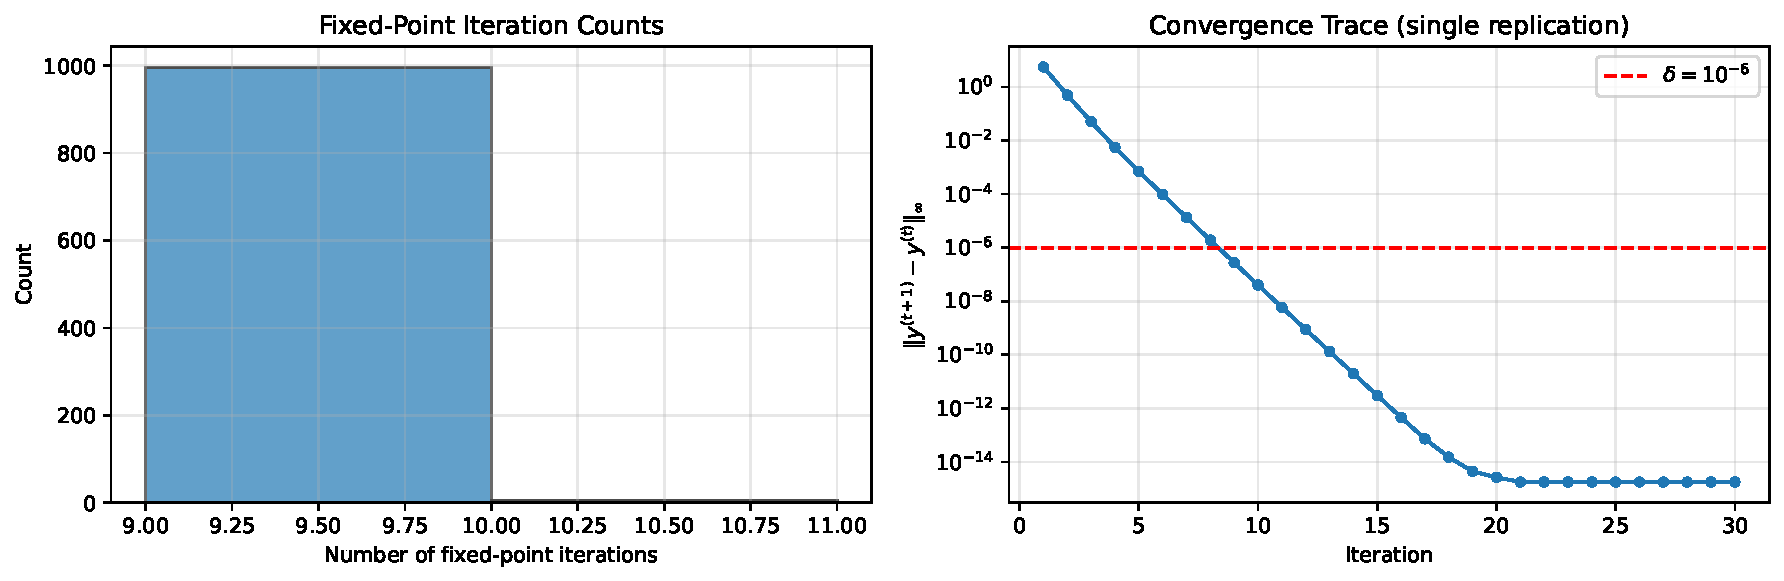
\includegraphics[width=\textwidth]{figures/mc_simul_fp_convergence.pdf}
    \caption[Fixed-point iteration convergence]{Visualisation of fixed-point iteration convergence across the $R = 1{,}000$ Monte Carlo replications. The left panel shows a histogram of the number of iterations to convergence with a tolerance of $\delta = 10^{-6}$. The right panel shows the geometric decrease in the maximum absolute change $\|\vect{y}^{(t+1)} - \vect{y}^{(t)}\|_\infty$ on a logarithmic scale, for a random replication.}
    \label{fig:mc_simul_fp_convergence}
\end{figure}

\begin{table}[htbp]
\centering
\caption[Monte Carlo results for FIML estimator of the simultaneous CoMO model]{Monte Carlo results for FIML estimator of the simultaneous CoMO model ($n = 500$, $R = 1{,}000$).}
\label{tab:mc_simul_results}
\begin{tabular}{lcccccc}
\toprule
Parameter & True & Mean Est. & Bias & Std(Est.) & Mean SE & Coverage \\
\midrule
$\beta_0$ & 3.50 & 3.4675 & $-0.0325$ & 0.8554 & 0.8274 & 0.952 \\
$\beta_1$ & 0.35 & 0.3483 & $-0.0017$ & 0.0778 & 0.0772 & 0.960 \\
$\beta_2$ & $-0.15$ & $-0.1437$ & 0.0063 & 0.1017 & 0.0970 & 0.938 \\
$\gamma_0$ & 7.00 & 7.0404 & 0.0404 & 0.6088 & 0.6027 & 0.951 \\
$\gamma_1$ & $-0.50$ & $-0.5027$ & $-0.0027$ & 0.0832 & 0.0823 & 0.943 \\
$\gamma_2$ & $-0.80$ & $-0.7998$ & 0.0002 & 0.0943 & 0.0946 & 0.952 \\
$\gamma_3$ & 0.25 & 0.2453 & $-0.0047$ & 0.0626 & 0.0627 & 0.942 \\
$\sigma_u^2$ & 1.44 & 1.4441 & 0.0041 & 0.1031 & 0.1023 & 0.951 \\
$\sigma_\varepsilon^2$ & 1.00 & 1.0008 & 0.0008 & 0.0677 & 0.0697 & 0.962 \\
\bottomrule
\end{tabular}
\end{table}

The mean estimates and biases show that the FIML estimator is approximately unbiased for all nine parameters. The largest bias is $0.040$ for $\gamma_0$, with $\beta_0$ also showing higher bias than the other parameters. We point to the discussion in Section~\ref{sec:mc:ml_screen} for why the intercepts have slightly higher bias and also why they have higher standard errors. We note that this is unproblematic and that the biases are still low. The Std(Est.) and Mean SE values are in close agreement for all parameters, and coverage is also close to the nominal 95\% across the board. This indicates that the standard errors based on the numerical Hessian are well-calibrated, and correctly capture the true sampling variability.

The coverages of $93.8\%$ for $\beta_2$ and $96.2\%$ for $\sigma_\varepsilon^2$ are the furthest from the nominal $95\%$. However, the Monte Carlo standard error for a $95\%$ coverage rate is approximately $\sqrt{0.95 \times 0.05/1{,}000} \approx 0.69$ percentage points when $R = 1{,}000$. Thus, $93.8\%$ and $96.2\%$ are about $1.7$ Monte Carlo standard errors from the nominal level, which is only a mild deviation.

In Figure~\ref{fig:mc_simul_hist_fiml} we plot histograms for estimates of all parameters. This gives a visual confirmation that the distributions of estimates are approximately symmetric and centred on the true values.

\begin{figure}[htbp]
    \centering
    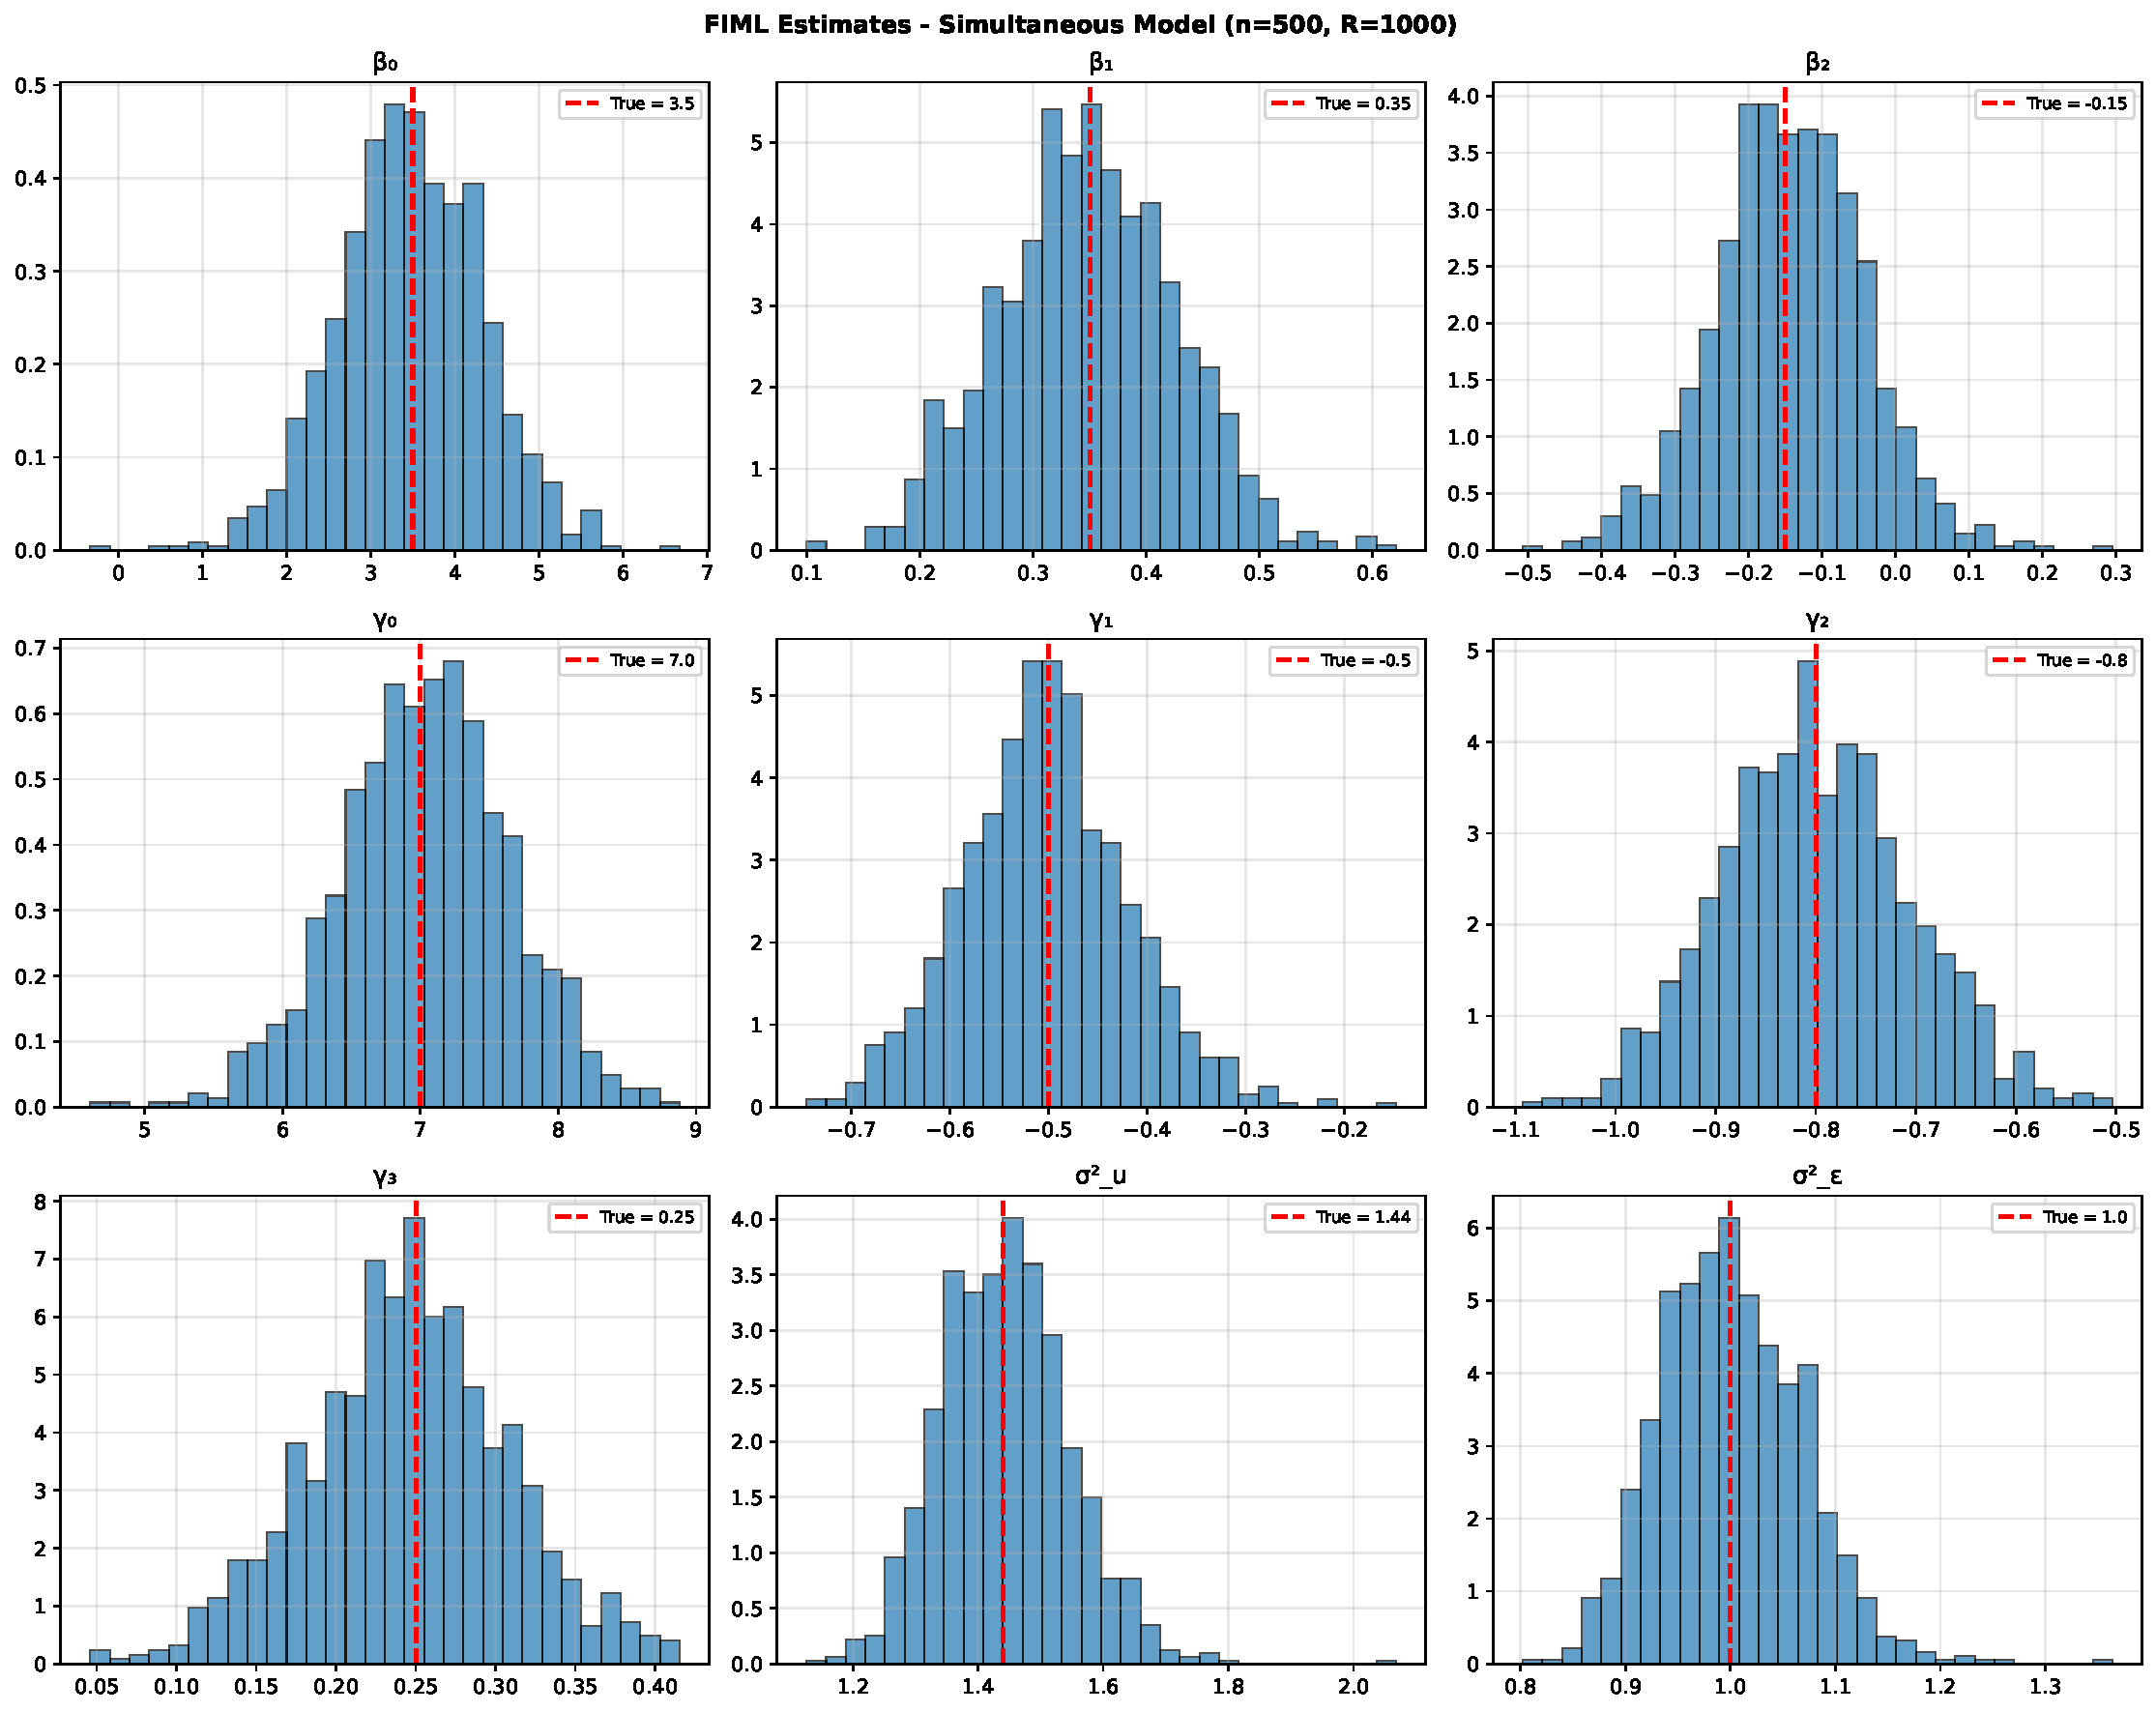
\includegraphics[width=\textwidth]{figures/mc_simul_hist_fiml.pdf}
    \caption[Histograms of FIML estimates]{The histograms display the FIML estimates for all nine parameters across the $R = 1{,}000$ Monte Carlo replications. The true parameter values are marked by red dashed lines. The histograms show approximate unbiasedness of the FIML estimators as the distributions are centred near the true values.}
    \label{fig:mc_simul_hist_fiml}
\end{figure}

\subsection{Assessment of Standard Errors}
\label{sec:simul:mc_se}
We now further assess the standard errors calculated by the numerical Hessian approximation. We do this through examining $z$-scores, and also through rejection rates from Wald tests of $H_0: \theta_k = \theta_k^0$, with $\theta_k^0$ the true parameter value. Under correct calibration of standard errors we expect the $z$-scores to be approximately standard normally distributed, and the empirical rejection rates at the $5\%$ level to be close to $0.05$.

This is exactly what we see. The results of the Wald tests are reported in Table~\ref{tab:mc_simul_rejection}, and show rejection rates hovering around the nominal 0.05 level. As in the analysis of Chapter~\ref{chap:monte_carlo}, we plot histograms of FIML $z$-scores in Figure~\ref{fig:mc_simul_zscore_hist}, and provide summary statistics in Table~\ref{tab:mc_simul_zscores}. Both the figure and summary statistics provide further evidence of proper calibration of Hessian-based standard errors: the $z$-scores are approximately standard normally distributed. All means are within $0.11$ of zero, and all standard deviations are within $0.04$ of one. Lastly, the values of skewness and kurtosis are small, with the largest in magnitude being $-0.292$ for skewness and $-0.271$ for kurtosis. These results correspond well with the coverages of Table~\ref{tab:mc_simul_results}, and confirm that the numerical Hessian-based standard errors are well-calibrated.

\begin{table}[htbp]
\centering
\caption[Empirical rejection rates for FIML Wald tests]{Empirical rejection rates at the $5\%$ level for FIML Wald tests ($n = 500$, $R = 1{,}000$, nominal: 0.05). Calculated as the Type I error rate under the null hypothesis that each parameter equals its true value.}
\label{tab:mc_simul_rejection}
\begin{tabular}{lc}
\toprule
Parameter & Rejection Rate \\
\midrule
$\beta_0$ & 0.048 \\
$\beta_1$ & 0.040 \\
$\beta_2$ & 0.062 \\
$\gamma_0$ & 0.049 \\
$\gamma_1$ & 0.057 \\
$\gamma_2$ & 0.048 \\
$\gamma_3$ & 0.058 \\
$\sigma_u^2$ & 0.049 \\
$\sigma_\varepsilon^2$ & 0.038 \\
\bottomrule
\end{tabular}
\end{table}

\begin{figure}[htbp]
    \centering
    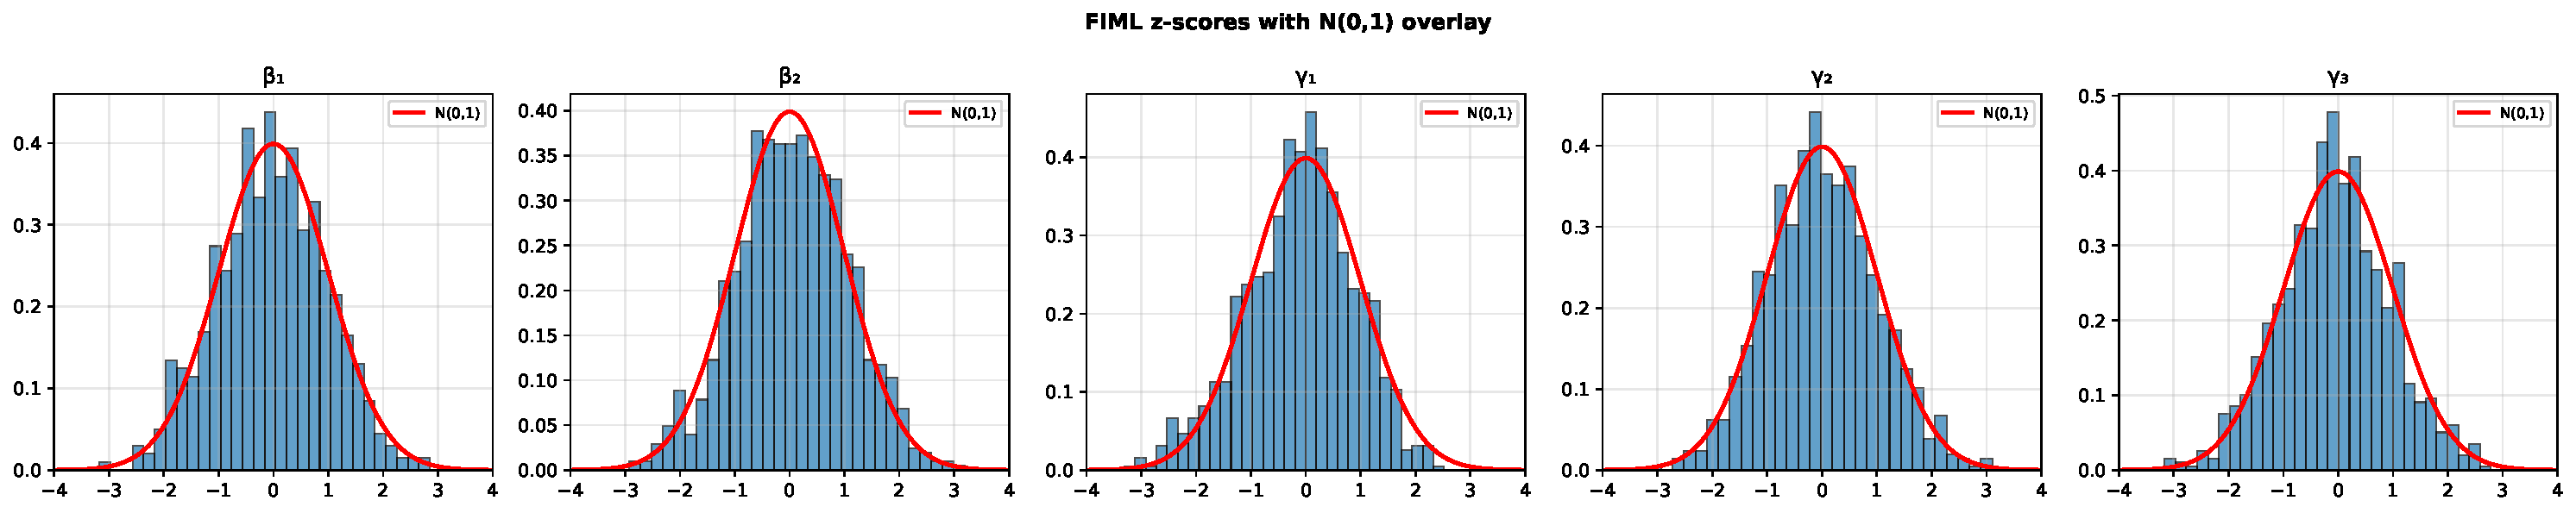
\includegraphics[width=\textwidth]{figures/mc_simul_zscore_hist.pdf}
    \caption[Histograms of FIML $z$-scores with $\N(0,1)$ overlays]{Histograms of FIML $z$-scores for the $R = 1{,}000$ Monte Carlo replications. Histograms are shown for the key parameters $\beta_1$, $\beta_2$, $\gamma_1$, $\gamma_2$, and $\gamma_3$. Red lines show overlays with $\N(0,1)$ densities. The approximate standard normal distribution of the $z$-scores signifies good calibration of the numerical Hessian-based standard errors.}
    \label{fig:mc_simul_zscore_hist}
\end{figure}

\begin{table}[htbp]
\centering
\caption[Summary statistics of FIML $z$-scores]{Summary statistics of FIML $z$-scores ($n = 500$, $R = 1{,}000$).}
\label{tab:mc_simul_zscores}
\begin{tabular}{lcccc}
\toprule
Parameter & Mean($z$) & Std($z$) & Skewness & Kurtosis \\
\midrule
$\beta_0$ & $-0.013$ & 1.002 & 0.061 & $-0.271$ \\
$\beta_1$ & $-0.037$ & 0.996 & $-0.041$ & $-0.257$ \\
$\beta_2$ & 0.054 & 1.018 & $-0.053$ & $-0.148$ \\
$\gamma_0$ & 0.110 & 1.000 & 0.186 & $-0.083$ \\
$\gamma_1$ & $-0.105$ & 0.997 & $-0.257$ & $-0.095$ \\
$\gamma_2$ & 0.003 & 0.994 & 0.099 & $-0.129$ \\
$\gamma_3$ & $-0.068$ & 0.999 & $-0.020$ & 0.018 \\
$\sigma_u^2$ & $-0.054$ & 1.007 & $-0.292$ & 0.240 \\
$\sigma_\varepsilon^2$ & $-0.084$ & 0.960 & $-0.240$ & $-0.124$ \\
\bottomrule
\end{tabular}
\end{table}

\subsection{Bias from Ignoring Feedback}
\label{sec:simul:mc_bias}
We now move on to testing the bias incurred when the recursive CoMO model (which assumes $\beta_2 = 0$) is used to estimate data generated from the simultaneous CoMO model ($\beta_2 = -0.15$). This is an important validation for the usefulness of the simultaneous CoMO model.

We generate data according to the DGP of the simultaneous CoMO model, using the parameters of Table~\ref{tab:mc_simul_params}, and then estimate parameters using both the FIML estimator and the now misspecified recursive ML estimators of Chapter~\ref{chap:estimation}. We report the results in Table~\ref{tab:mc_bias_comparison}. Here, $\beta_0$ and $\beta_2$ are omitted from the comparison. These are not comparable, as $\beta_2$ is not present in the recursive CoMO model, and $\beta_0$ has differing true values ($2.5$ in the recursive CoMO model, $3.5$ in the simultaneous CoMO model).

\begin{table}[htbp]
\centering
\caption[Bias comparison of recursive ML vs.\ FIML estimators]{Bias comparison of recursive ML vs.\ FIML estimators, fit on data from the simultaneous CoMO model ($n = 500$, $R = 1{,}000$). The FIML numbers are an independent Monte Carlo run, so there are small numerical differences from Table~\ref{tab:mc_simul_results} due to Monte Carlo sampling variability.}
\label{tab:mc_bias_comparison}
\begin{tabular}{lcccccccc}
\toprule
& & \multicolumn{3}{c}{Recursive ML} & \multicolumn{3}{c}{FIML} \\
\cmidrule(lr){3-5} \cmidrule(lr){6-8}
Parameter & True & Bias & Std(Est.) & RMSE & Bias & Std(Est.) & RMSE \\
\midrule
$\beta_1$ & 0.35 & 0.0735 & 0.0605 & 0.0952 & $-0.0034$ & 0.0772 & 0.0773 \\
$\gamma_0$ & 7.00 & 0.4106 & 0.4914 & 0.6404 & 0.0358 & 0.5872 & 0.5883 \\
$\gamma_1$ & $-0.50$ & $-0.0870$ & 0.0510 & 0.1009 & $-0.0003$ & 0.0816 & 0.0816 \\
$\gamma_2$ & $-0.80$ & 0.0304 & 0.0959 & 0.1006 & 0.0003 & 0.0959 & 0.0959 \\
$\gamma_3$ & 0.25 & $-0.0131$ & 0.0589 & 0.0603 & $-0.0057$ & 0.0604 & 0.0607 \\
$\sigma_u^2$ & 1.44 & 0.0736 & 0.1028 & 0.1265 & $-0.0025$ & 0.1040 & 0.1040 \\
$\sigma_\varepsilon^2$ & 1.00 & $-0.0218$ & 0.0623 & 0.0660 & 0.0012 & 0.0703 & 0.0704 \\
\bottomrule
\end{tabular}
\end{table}

The results show exactly what was expected: ignoring the feedback from WB to SMU biases the results of estimating with the recursive ML method on data from the simultaneous CoMO model. In particular, the recursive ML estimator exhibits a bias of $0.074$ in its estimation of $\beta_1$ (relative bias: $21\%$), and $0.411$ in the estimation of $\gamma_0$ (relative bias: $6\%$). Both biases are more than an order of magnitude higher than the FIML estimator equivalents. It also overestimates the magnitude of the direct SMU effect on WB ($\gamma_1$) by $0.087$. The recursive ML estimator for $\sigma_u^2$ also shows an upward bias of $0.074$ (relative bias: $5\%$). The FIML estimator, on the other hand, has negligible biases for all parameters.

The results can be explained by a misattribution occurring in the recursive ML estimator. When there is feedback from WB to SMU, we introduce a correlation between $\vect{s}$ and $\vect{\varepsilon}$. While the FIML estimator can account for this, the recursive ML estimator will misattribute this correlation. This can also be seen as a form of omitted-variable bias, as the omitted $\beta_2 y_i$ makes the effective error of the SMU equation $\tilde{u}_i = u_i + \beta_2 y_i$. This extra variation must be absorbed into the other regressors. For example, a negative WB shock ($\varepsilon_i < 0$) leads to a decrease in $y_i$ and corresponding increase in $s_i$ through $\beta_2$. This also raises $\sbar_j$, which inflates $\hat{\beta}_1$ even though there is no true increase in peer conformity. In this way the unmodelled feedback biases $\hat{\beta}_1$ from the recursive ML estimator. In the WB equation, $\vect{s}$ is endogenous as $s_i$ depends negatively on $\varepsilon_i$ through $\beta_2 y_i$. This negative correlation biases $\hat{\gamma}_1$ further away from zero. Lastly, the effective errors $\tilde{u}_i = u_i + \beta_2 y_i$ inflate the recursive ML estimate of $\sigma_u^2$, as it captures additional variance from the unmodelled feedback.

The RMSE values of the two models are quite closely aligned. Here there are two competing effects at play: a decrease in RMSE for the recursive CoMO model from fewer estimated parameters, and an increase in RMSE caused by biased estimates. For the parameters with the highest bias ($\beta_1$, $\gamma_0$, $\gamma_1$, $\sigma_u^2$), this leads to the FIML estimator having lower RMSE despite the additional parameter. Here, the largest difference is in $\sigma_u^2$, where the recursive RMSE is $22\%$ higher than the FIML RMSE ($0.127$ versus $0.104$). This corresponds to a relatively large difference in bias between the recursive and FIML estimates. However, for the parameters with lower bias ($\gamma_2$, $\gamma_3$, $\sigma_\varepsilon^2$), the RMSE values are approximately equal or lower for the recursive estimator.

\subsection{Size and Power of the Wald Test for Feedback}
\label{sec:simul:wald_test}
The nested nature of the recursive CoMO model within the simultaneous CoMO model (when $\beta_2 = 0$) allows us to test for the presence of feedback using a Wald test. This section assesses both the size of the test under $H_0: \beta_2 = 0$, and the power of the test against $\beta_2 = -0.15$. We also report numbers on the efficiency cost of using FIML over the recursive CoMO model.

We begin with the size of the test under the null hypothesis. We use the test statistic $z = \hat{\beta}_2 / \widehat{\text{SE}}(\hat\beta_2)$. Under $H_0$, this is approximately standard normally distributed. We run separate Monte Carlo simulations with the DGP of the recursive CoMO model ($\beta_0 = 2.5$, $\beta_2 = 0$, otherwise see Table~\ref{tab:mc_simul_params}), and $n = 500$ and $R = 1{,}000$ as before. Then, we estimate using the FIML model on this data. A rejection of this test signifies the presence of feedback from WB to SMU, implying a need for the simultaneous CoMO model. The results are presented in Table~\ref{tab:mc_wald_size}, and show that the test has approximately correct size. At all reported levels, the rejection rates are close to nominal. For the $5\%$ level, the discrepancy is the largest, with test rejections in $4.0\%$ of samples. However, with a Monte Carlo $95\%$ interval of $[3.6\%, 6.4\%]$, this is well within expected sampling variability.

\begin{table}[htbp]
\centering
\caption[Size of Wald test for $H_0: \beta_2 = 0$]{Size of Wald test for $H_0: \beta_2 = 0$ under $H_0$ ($n = 500$, $R = 1{,}000$).}
\label{tab:mc_wald_size}
\begin{tabular}{lc}
\toprule
Significance Level & Rejection Rate (Size) \\
\midrule
10\% & 0.092 \\
5\% & 0.040 \\
1\% & 0.011 \\
\bottomrule
\end{tabular}
\end{table}

This same simulation allows us to quantify the efficiency cost of using FIML when the DGP corresponds to the recursive CoMO model. We report the FIML standard deviations and mean SEs for the five shared parameters under the recursive DGP in Table~\ref{tab:mc_simul_efficiency}. We also include the corresponding values from the recursive ML simulation from Chapter~\ref{chap:monte_carlo}. The results show that there is increased variance in the sampling distributions of $\beta_1$, $\gamma_0$, and $\gamma_1$, which might be caused by the fact that FIML treats $\vect{s}$ as endogenous. The values for $\gamma_2$ and $\gamma_3$ are very similar for the two models. Coverage is close to nominal for all the parameters. We will discuss the practical implications of these results in Section~\ref{sec:simul:comparison}.

\begin{table}[htbp]
\centering
\caption[Efficiency cost of FIML vs.\ recursive estimators under the recursive DGP]{Comparison of efficiency cost of FIML and recursive CoMO estimators under the recursive CoMO DGP ($\beta_2 = 0$, $n = 500$, $R = 1{,}000$). The values for the recursive CoMO model are the same as in Tables~\ref{tab:mc_screen_ml} and~\ref{tab:mc_ml_results} of Chapter~\ref{chap:monte_carlo}.}
\label{tab:mc_simul_efficiency}
\begin{tabular}{lcccccc}
\toprule
& & \multicolumn{2}{c}{Recursive ML} & \multicolumn{3}{c}{FIML} \\
\cmidrule(lr){3-4} \cmidrule(lr){5-7}
Parameter & True & Std(Est.) & Mean SE & Std(Est.) & Mean SE & Coverage \\
\midrule
$\beta_1$    &  0.35 & 0.0646 & 0.0629 & 0.0779 & 0.0806 & 0.957 \\
$\gamma_0$   &  7.00 & 0.5050 & 0.5074 & 0.5658 & 0.5660 & 0.950 \\
$\gamma_1$   & $-0.50$ & 0.0538 & 0.0548 & 0.0848 & 0.0845 & 0.950 \\
$\gamma_2$   & $-0.80$ & 0.0938 & 0.0947 & 0.0976 & 0.0953 & 0.939 \\
$\gamma_3$   &  0.25 & 0.0623 & 0.0622 & 0.0630 & 0.0629 & 0.942 \\
\bottomrule
\end{tabular}
\end{table}

We now assess the empirical power of the test, investigating how often it correctly rejects $H_0$ when $\beta_2 = -0.15$. We use the main simulation design of this chapter with $\beta_2 = -0.15$. For each replication, we calculate the test statistic $z = \hat{\beta}_2 / \widehat{\text{SE}}(\hat\beta_2)$, and check whether $|z| > z_{1-\alpha/2}$ for each significance level. We note that one-sided tests could also be applied if warranted by prior knowledge, and that these would have increased power. The results of our simulations are reported in Table~\ref{tab:mc_wald_power}, and are the following: at the $10\%$, $5\%$, and $1\%$ levels, the rejection rates are $46.4\%$, $33.7\%$, and $15.1\%$, respectively. We also have that the mean test statistic is $\bar{z} = -1.52$, with $|\bar{z}| = 1.52$ below the two-sided $5\%$ critical value of $1.96$.

\begin{table}[htbp]
\centering
\caption[Power of Wald test for $H_0: \beta_2 = 0$ against $\beta_2 = -0.15$]{Power of Wald test for $H_0: \beta_2 = 0$ against $\beta_2 = -0.15$ ($n = 500$, $R = 1{,}000$).}
\label{tab:mc_wald_power}
\begin{tabular}{lc}
\toprule
Significance Level & Rejection Rate (Power) \\
\midrule
10\% & 0.464 \\
5\% & 0.337 \\
1\% & 0.151 \\
\bottomrule
\end{tabular}
\end{table}

These are moderate to low powers, which reflect the difficulty of detecting feedback (especially with low significance values) when we have $n = 500$ observations and an Erd\H{o}s--R\'enyi network with density $p = 0.01$. With this setup and the value $\beta_2 = -0.15$, the signal-to-noise ratio is too low for reliable detection in a single sample.

The unreliable detection can be verified through a direct calculation using $\widehat{\text{SE}}(\hat\beta_2) = 0.097$ from Table~\ref{tab:mc_simul_results}. Under the alternative, $z$ is approximately $\N(|\beta_2|/\widehat{\text{SE}}(\hat\beta_2), 1) \approx \N(1.55, 1)$, so the chance of $|z| > 1.96$ is approximately $\Phi(-0.41) \approx 0.34$. This matches the observed rejection rate of $33.7\%$ and $\bar z = -1.52$ closely.

The moderate power of $33.7\%$ at the $5\%$ level means that an application of the model to a single network dataset of $n = 500$ where true $\beta_2 = -0.15$ would fail to reject $H_0$ around two-thirds of the time. This is not due to any fault with the test, but is a consequence of the difficulty of the estimation problem. Whether or not the test rejects, we still retrieve unbiased estimates of all parameters when applying the FIML estimator. In practice, if the presence of feedback is in question, data can help answer the question by fitting the FIML estimator without introducing bias.

The results of the size and power of the Wald test show that the test is well-calibrated. It rejects at approximately nominal rates under $H_0$, and has expected moderate power. Larger sample sizes would increase the power. In practice, the test can be used to give information on whether or not the potential for feedback should be modelled. Including this in the model protects against the bias of an omitted variable, but reduces the efficiency of the estimator.

%% Section 7.4: Discussion
\section{Discussion}
\label{sec:simul:discussion}
This section briefly compares the recursive and simultaneous CoMO models, explains why we have not developed instrumental variables estimation for the simultaneous CoMO model, and discusses limitations and future work. This leads into the further discussion of Chapter~\ref{chap:discussion_conclusion}.

\subsection{Comparison of Recursive and Simultaneous CoMO Models}
\label{sec:simul:comparison}
Table~\ref{tab:recursive_vs_simul} provides an overview of the differences between the recursive and simultaneous CoMO models.

\begin{table}[htbp]
\centering
\caption[Comparison of recursive and simultaneous CoMO models]{Comparison of recursive and simultaneous CoMO models.}
\label{tab:recursive_vs_simul}
\small
\begin{tabular}{lcc}
\toprule
Feature & Recursive & Simultaneous \\
\midrule
Allows $y \to s$ feedback & No & Yes \\
Number of parameters & 8 & 9 \\
Closed-form reduced form & Yes & No (fixed-point) \\
ML estimation & Concentrated, 1D + 1D & Concentrated, 5D (warm-started) \\
Analytical Hessian & Derived (Chapter~\ref{chap:estimation}) & Not yet derived \\
Standard errors & Analytical & Numerical \\
IV identification & WB equation only & Not available (see Remark~\ref{rem:simul_no_iv}) \\
Monte Carlo validation & $R = 1{,}000$ (Ch.~\ref{chap:monte_carlo}) & $R = 1{,}000$ (this chapter) \\
\bottomrule
\end{tabular}
\end{table}

The simultaneous CoMO model introduces complexity through the $y \to s$ feedback, requiring the estimation of an additional parameter and increasing the dimensionality of the ML estimation. Instead of two one-dimensional optimisations, it requires solving a five-dimensional problem. It also introduces additional computational cost in the likelihood evaluations, which require a sparse log-determinant of the Schur complement. We also lack analytical standard errors and IV identification for comparison. This yields a trade-off between realism and robustness on the one hand, and computational cost on the other. If the feedback does exist, the simultaneous CoMO model does not exhibit omitted-variable bias (see Section~\ref{sec:simul:mc_bias}). If there is no such feedback, and the recursive CoMO model is true, estimating the simultaneous CoMO model is less efficient. This is because the model treats $\vect{s}$ as endogenous, which makes the sampling distributions of $\hat{\beta}_1$, $\hat{\gamma}_0$, and $\hat{\gamma}_1$ more variable (see Table~\ref{tab:mc_simul_efficiency}). The cost is most severe for the parameters $\beta_1$, $\gamma_0$, and $\gamma_1$, for which the FIML standard deviations are about $21\%$, $12\%$, and $58\%$ higher, respectively. For $\gamma_2$ and $\gamma_3$ the increases are small. However, coverage is still near $95\%$ for the FIML estimator even if the recursive CoMO model is true.

Using the FIML estimator also gives unbiased estimates, even when there is no feedback. Thus, in practice, if there is substantive uncertainty about whether feedback is present, fitting the FIML estimator as a robustness check can be worth it despite the efficiency cost. The Wald test for $H_0: \beta_2 = 0$ was shown to have moderate power when $n = 500$. While still providing information, non-rejection of the test is thus weak evidence for the absence of feedback. If there is good reason to believe that there is no feedback, or the efficiency gain is substantial, the recursive CoMO model is preferred.

\begin{remark}[Absence of IV Estimation]
\label{rem:simul_no_iv}
We include a remark on why IV estimation is not feasible for the simultaneous CoMO model in the current specification. For the recursive CoMO model, network instruments allowed for successful 2SLS estimation of the WB equation (see Section~\ref{sec:est:wb_2sls}). However, in the simultaneous CoMO model, the feedback makes all the non-intercept regressors endogenous. Both $\vect{s}$ and $\vect{c}(\vect{s})$ are correlated with the errors from the WB equation. This leaves us without any valid instruments usable for identification. In future work this could be addressed through the addition of exogenous individual-level covariates. This is similar to the SMU equation of the recursive CoMO model (see Section~\ref{sec:est:screen_2sls}). Instead of IV estimation, we thus only rely on the FIML approach, exploiting the distributional assumptions and the Jacobian structure for identification.
\end{remark}

\subsection{Limitations and Future Work}
\label{sec:simul:future}
We end the chapter with some limitations of the simultaneous CoMO model. These also provide directions for future work.

\begin{enumerate}
    \item \textbf{Analytical Hessian.} In our current implementation, standard errors are computed with a numerical Hessian approach requiring $O(p^2)$ likelihood evaluations. Both the speed and reliability of standard error computation could be improved by deriving the analytical Hessian of the FIML likelihood. Such a derivation would be algebraically involved, but is feasible in principle. This is left for future work.

    \item \textbf{Broader Monte Carlo validation.} In Chapter~\ref{chap:monte_carlo} we provided broad Monte Carlo validation of the recursive CoMO model estimators, investigating both the influence of varying sample sizes and network densities. This chapter provided an initial smaller Monte Carlo study with $R = 1{,}000$, which gave good evidence on both bias and coverage. However, a broader validation of the FIML estimator would strengthen confidence in it.

    \item \textbf{IV identification.} Remark~\ref{rem:simul_no_iv} discusses the lack of IV identification of the simultaneous CoMO model. Future work could develop IV estimators through extending the model with exogenous individual-level covariates. Exploring how the CoMO non-linearity could be exploited for identification is a different potential avenue for future research.

    \item \textbf{Sharper equilibrium conditions.} In Proposition~\ref{prop:contraction} we provided a sufficient condition for the Banach fixed-point theorem to guarantee the existence and uniqueness of the equilibrium. However, this constant~\eqref{eq:contraction_constant} is an upper bound that covers even the worst-case scenarios of operator norm estimates. Further work could sharpen this bound through, for example, exploiting spectral properties of the network $\mat{G}$, allowing for a stronger absolute influence of WB on SMU in the model.
\end{enumerate}

We have now developed the simultaneous CoMO model as well as the recursive specification of Chapter~\ref{chap:model}. This concludes the analytical framework of the thesis. In Chapter~\ref{chap:discussion_conclusion}, we return to the motivating research question, and combine these results with the ABM diagnosis of Chapter~\ref{chap:abm} to discuss the findings of the thesis.


% Chapter 8: Discussion and Conclusion
%% Chapter 8: Discussion and Conclusion

\chapter{Discussion and Conclusion}
\label{chap:discussion_conclusion}
This chapter wraps up the thesis. We begin with a synthesis of our findings in light of the motivating research question. Then we look at the contributions of the thesis relative to existing literature, and discuss the gap between the ABMs of Chapter~\ref{chap:abm} and the analytical modelling of subsequent chapters. We end by discussing the implications for SMU--WB research, along with limitations and directions for future work.

%% Section 8.1: Synthesis of Findings
\section{Synthesis of Findings}
\label{sec:discussion_conclusion:synthesis}
We now return to the motivating research question of Section~\ref{sec:intro:motivation}:
\begin{quote}
\emph{What is the causal influence of social media use on well-being?}
\end{quote}

The answer is that the causal influence of SMU on WB remains unclear. This thesis has not tried to answer the question directly, but instead shows that omission of network effects might be a key reason why the existing evidence cannot answer it. We developed network-aware models for future empirical estimation.

In Chapter~\ref{chap:introduction} we argued that the field of research tackling this question is affected by the methodological problem of not modelling network effects. This is because the standard statistical methods of the field, such as cross-sectional OLS, panel data with fixed effects, and randomised controlled trials (RCTs), fail when applied to networked data. In particular, we identified three statistical problems that arise when network effects are neglected: \emph{endogeneity} (peer outcomes enter the DGP but not the regression), \emph{relative effects} (differences between individual and peer behaviour have an effect on WB), and \emph{spillovers} (changes in one unit propagate through the network, breaking independence). The endogeneity problem relates to the \emph{reflection problem} of \textcite[Sec.~2]{Manski1993}, which is the problem of separately identifying endogenous, contextual, and correlated peer effects within a linear-in-means formulation.

We now give a synthesis of how the thesis arc follows these problems, from the problem diagnosis of Chapter~\ref{chap:abm} to the solutions developed in Chapters~\ref{chap:model}--\ref{chap:simultaneous}.

\subsection{Diagnosis: Standard Methods Fail Under Network Effects}

We begin by recounting the diagnosis of Chapter~\ref{chap:abm}, which applied ABMs to networked data. We defined three scenarios: a reference scenario, a scenario with the CoMO effect using a global mean, and a Network \& CoMO scenario based on peer reference. In the reference scenario, standard methods recovered the true effect. However, when the true DGP was networked, simulations showed attenuation of the true effect across the board. In the global CoMO scenario the methods exhibited relative biases of roughly $20\%$--$26\%$, with the cross-sectional OLS and RCT biases increasing further in the Network \& CoMO scenario (see Table~\ref{tab:abm_summary}). The most noticeable result was that RCTs, often regarded as the gold standard of causal inference, were the \emph{most} biased method in our simulations, with a relative bias of $31.9\%$ in the Network \& CoMO scenario (but note that this is subject to the $n$/density caveat from Section~\ref{sec:abm:methods}). The explanation is the independence required by the SUTVA Assumption~\ref{ass:sutva}. When we treat some agents with less SMU, this has a spillover effect on others through lowering their peer reference level. This attenuates the contrast between the groups, biasing estimates downwards.

In addition to showing that standard methods are biased under network effects, we used the complexity allowed for by ABMs to demonstrate Simpson's Paradox in Section~\ref{sec:abm:simpsons}. Implementing a delayed-decline mechanism allowed us to show how a DGP with a negative influence of SMU on WB could still lead to the paradox: cross-sectional regression at any single time point shows a positive association between SMU and WB, while at a population level, average SMU is increasing whereas average WB is declining. This shows the difficulty research in this field faces, as someone applying the seemingly reasonable procedure of cross-sectional regression might actually retrieve estimates with the opposite sign to the true effect. As many studies in the SMU--WB field rely on exactly such single-survey regressions, these results, together with the bias results, suggest a potential explanation for the conflicting estimates in the literature: substantial harms in \textcite{Twenge2018} and \textcite{Haidt2024}, and negligible effects in \textcite{Orben2019}. This divergence in results might be due to methodological limitations of methods not taking network effects into account.

Our finding of bias towards zero applies most strongly to studies that report small effects. If the underlying effect is actually large, but this type of bias or attenuation is present, we would expect to find small effects. We note that our simulations provide evidence for the plausible direction of bias in general for studies not taking network effects into account, which does not necessarily apply to any individual study.

\subsection{Solution: A Network-Aware Model with Formal Estimation}

We now move on to the solution: explicit modelling of network effects. In Chapter~\ref{chap:model} we introduced the recursive CoMO model, which lets peers influence the individual through three channels: peer conformity in SMU through $\beta_1$ in the SMU equation, and the CoMO effect and endogenous peer-WB spillover through $\gamma_2$ and $\gamma_3$ in the WB equation. This model addresses the three statistical problems caused by neglecting network effects. We recognise $\mat{G}\vect{y}$ as endogenous, and handle it accordingly when developing estimators. Relative peer effects are formalised and captured through the asymmetric CoMO term. Spillovers are made explicit in the peer-outcome term of the reduced form, and accounted for in estimation. The recursive structure makes the equations separately estimable under Assumption~\ref{ass:error_indep}, which simplifies estimation.

The CoMO term is non-linear, but does not cause problems in estimation. Instead, it provides us with the additional excluded instrument $\mat{G}\vect{c}$, which a standard SAR model does not usually have. We can use this as an instrument because the max operator makes $\vect{c}$ generically linearly independent of $\vect{1}$ and $\vect{s}$. This is formalised as a full-column-rank condition on the design matrix $\mat{X} = [\vect{1}, \vect{s}, \vect{c}]$. In Proposition~\ref{prop:wb_identification}, we use this instrument together with $\mat{G}^2\vect{s}$ to show that the WB structural parameters are identified via the IV route under the \textcite[Prop.~1]{Bramoulle2009} condition that $\{\mat{I}, \mat{G}, \mat{G}^2\}$ are linearly independent. We also show how the Gaussian form of the likelihood can identify the full WB parameter vector (Proposition~\ref{prop:wb_ml_identification}).

We developed both ML and 2SLS estimators for the model in Chapter~\ref{chap:estimation}, along with the analytical Hessians. For the SMU equation, we developed only the ML estimator, as the lack of exogenous covariates makes 2SLS unavailable. The estimators have different properties. The ML estimator requires normality, but is asymptotically efficient when this holds. The 2SLS estimator is more robust to distributional misspecification, but is generally less efficient. Applying both estimators is informative: agreement between them strengthens confidence in estimates, while disagreement requires consideration of whether there are weak instruments or an error in the specification.

\subsection{Validation and Extension}

The developed estimators were validated through Monte Carlo simulations in Chapter~\ref{chap:monte_carlo}. The main result is the success of both estimators in recovering true parameters. They have low bias, standard errors declining at an expected rate of $1/\sqrt{n}$, and roughly nominal confidence interval coverage. The analytical Hessians were verified to match closely with numerical estimates. The simulations also confirmed the theoretical properties of the two estimators, showing the increased efficiency of the ML estimator across the simulation studies. The relative efficiencies ranged from $1.2\times$ to $5\times$ across the parameters, with $\gamma_3$ having the largest gap, likely due to noise caused by weak instruments. When normality seems reasonable, these results clearly favour the ML estimator. Another set of notable results with practical consequences comes from the density study. These showed that as the density of the network increased, instrument strength weakened. From the least to most dense networks tested, the first-stage $F$-statistic fell from roughly 15 to 3.5, and RMSE for $\gamma_3$ went from $0.305$ to $2.759$ for the 2SLS estimator. The ML estimator performance also degraded, but at a modest rate (see Section~\ref{sec:mc:density}). Thus, for networks of modest to high density, which might include networks most likely to meet the data requirements of Section~\ref{sec:discussion_conclusion:data_requirements}, the ML estimator should be the primary estimator, with the 2SLS serving as a check of robustness.

Lastly, we extended the recursive CoMO model to the simultaneous CoMO model in Chapter~\ref{chap:simultaneous} by relaxing the recursive assumption. We allowed for feedback from WB to SMU through an additional parameter $\beta_2$ in the SMU equation. This led to a system without a closed-form reduced form, which required showing the existence of a unique equilibrium. We showed this in Proposition~\ref{prop:contraction}, together with the conditions under which fixed-point iteration converges to said equilibrium. We then developed an FIML estimator for the model, along with a Schur-complement simplification that exploits sparsity for computational efficiency. We provided an initial validation of the estimator with Monte Carlo simulations, which showed low bias and well-calibrated standard errors. Additionally, as the recursive CoMO model is nested in the simultaneous CoMO model as the special case of $\beta_2 = 0$, we applied a Wald test for detecting the need for the simultaneous CoMO model under a simultaneous DGP\@. The test size was validated, with test power being low to moderate in our simulation study.

%% Section 8.2: Contributions in Context
\section{Contributions in Context}
\label{sec:discussion_conclusion:contributions}
In Section~\ref{sec:intro:contributions} we outlined the six novel contributions made in this thesis. This section discusses these in light of the wider literature.

\textbf{(i) The ABM demonstration of bias and Simpson's Paradox} connects to the broader literature on interference and the SUTVA assumption \parencite[Sec.~2.1]{HudgensHalloran2008}, as well as to the tradition of using ABMs to understand social phenomena \parencite{Macy2002}. We are not aware of any prior studies quantifying bias in the SMU--WB setting under the CoMO mechanism. This thesis thus contributes by placing the SMU--WB question both in the frame of the interference literature and in the methodological tradition of understanding through simulated bottom-up dynamics.

\textbf{(ii) The recursive CoMO model} builds on psychological literature that has discussed social comparison since \textcite{Festinger1954}. Reframing the FOMO concept of \textcite[p.~1841]{Przybylski2013}, \textcite[Eqs.~1--2]{DahlFoldnesGronneberg2024} introduced the CoMO concept in the SMU--WB context and used a stylised linear mediation model to illustrate some of its consequences, with \textcite{DahlFoldnesGronneberg2026} extending the framing for policy applications. The contribution made in this thesis is the development of the concept into an identified component of a SAR model. We adapt the \textcite{Bramoulle2009} identification argument to show identification of the WB equation in the presence of the CoMO term.

\textbf{(iii) and (iv) The ML and 2SLS estimators} are developed in line with existing theory of maximum likelihood for SAR models of \textcite{Lee2004}, and the \textcite{Bramoulle2009} network instrument approach for 2SLS estimation. For the recursive CoMO model, our contribution is to adapt this theory to the two-equation structure with the non-linear CoMO term. Checking model robustness through applying both ML and 2SLS estimators is a known practice in spatial econometrics \parencite{LeSage2009}.

\textbf{(v) The Monte Carlo validation} of the estimators is applied to sample sizes relevant for empirical application. In particular, the density sensitivity study of Section~\ref{sec:mc:density} contributes an important insight, which is that 2SLS becomes unreliable when networks reach a certain density, making the ML estimator preferable for relevant applications.

\textbf{(vi) The simultaneous CoMO model} moves further away from the standard linear-in-means systems commonly treated in spatial econometrics, contributing an explicit uniqueness result based on Banach's fixed-point theorem. The previous SMU--WB literature does not provide \emph{a priori} knowledge of whether feedback from WB to SMU is negligible. Thus, this extension contributes by broadening the applicability of the developed framework, without sacrificing formal inference.

The contributions of this thesis are methodological, and application of the methods to real SMU--WB data remains future work (Section~\ref{sec:discussion_conclusion:limitations_future}).

%% Section 8.3: Bridging ABMs and Analytical Methods
\section{Bridging ABMs and Analytical Methods}
\label{sec:discussion_conclusion:gap}
A central approach of this thesis is the complementary application of ABM simulations and analytical inference. This section bridges the two, discussing their strengths and weaknesses.

ABMs can represent complexity in a way analytical methods cannot \parencite[Ch.~1]{Epstein2006}. In Chapter~\ref{chap:abm}, we set up heterogeneous agents with varying parameters and gave them learning rules, mean-reverting behaviour, delayed effects, and network-dependent CoMO\@. The simulations then evolved in complex ways according to these rules over time. This level of complexity in the DGP is intractable to model with analytical approaches. However, the real world might be closer to the complexity of ABMs than to that of analytical methods. Thus, ABMs can give insight into real-world dynamics that would otherwise be out of reach. In our case they are our diagnostic tool, as they show how network effects bias estimates of standard methods, as well as how such effects can lead to counterintuitive emergent results such as Simpson's Paradox.

Analytical methods allow for formal inference, letting us quantify uncertainty in a way not available with ABMs. For our recursive CoMO model of Chapters~\ref{chap:model}--\ref{chap:estimation}, this means that we have the properties of consistency and asymptotic normality, and we have available to us standard errors, confidence intervals, hypothesis tests, as well as conditions on identifiability. These allow us to draw more credible causal conclusions from a single observed dataset when the model assumptions hold. While the ABMs can diagnose bias issues under network effects, the analytical estimator gives us the underlying parameter estimates, together with measures of how precisely they have been estimated.

The gap between the two approaches is found in the complexity analytical approaches cannot handle, but which ABMs can. In our approach, the clearest gap is in dealing with complex temporal effects of agentic behaviour. For example, the CoMO mechanism is applied in the ABMs in a way that allows it to interact with learning and adaptation, generating feedback loops and other temporal dynamics. In our recursive CoMO model, the mechanism is static, capturing the CoMO an individual experiences at a single cross-section. We need this simplification to allow for identification and estimation, but it is arguably a strong assumption. Compared to the standard methods shown to be biased, our recursive CoMO model, and especially the simultaneous CoMO model of Chapter~\ref{chap:simultaneous}, allow for analytical modelling of peer effects. Thus, they can be seen as a start to narrowing the gap between ABMs and analytical approaches. However, the gap remains wide, and requires substantial further work to be closed.

We do not apply our analytical estimators directly to the ABM-generated data of Chapter~\ref{chap:abm}. This is because the DGP used for the ABMs is outside the parametric family of the recursive CoMO model, with temporal structure, learning rules, and heterogeneity in agents that break the model assumptions found in Section~\ref{sec:model:assumptions}. Developing analytical models fit for the DGP used in our ABMs requires substantial future work. In this thesis, we are content with validating our analytical estimators on the DGP they were designed for.

In our thesis, both approaches were used not only to draw the line from diagnosing with ABMs to analytical solutions, but also to illustrate that the gap persists. This strategy of using ABMs for diagnosis and analytical methods for inference could be applied more generally to areas where network effects are present, or where other effects require new estimation methods.

%% Section 8.4: Implications for SMU--WB Research
\section{Implications for SMU--WB Research}
\label{sec:discussion_conclusion:implications}
The finding that network effects can lead to bias, or even the wrong sign, in estimates of the relationship between SMU and WB when using standard methods gives a new reading of existing studies. The social nature of social media makes the presence of such effects plausible. Thus, the conflicting evidence in the current literature should not be read as conclusive evidence of either negligible or strong effects. Instead, it might be better to interpret this as an indication that network effects (or other unmodelled effects) are present, and that this leads to biased and inconsistent estimates.

The simulations in this thesis use parameters and network topologies that are not based on real data. Hence, we should be careful about over-interpreting the results. The bias magnitudes and sign-shift in the Simpson's Paradox illustration should therefore be taken as evidence that such effects are \emph{possible}, but not that these exact magnitudes or effects are present. Other unknown factors might be present, so the takeaway is the need for a careful evaluation to ensure appropriate modelling and interpretation of estimates.

The current research should also take into account the possibility that the CoMO mechanism is empirically relevant. While the mechanism has not yet been validated with real data, a true $\gamma_2 < 0$ in the population would require the field to adapt its approach. In that case, investigating the SMU--WB relationship requires a focus not only on the absolute usage of each individual, but also on how this compares to the use of their peers. For example, someone using social media for two hours per day could have higher well-being when their peers use it for one hour than if their peers use it for four, and we would need information on the peer usage to know the full story. This has consequences for the type of intervention designs future studies should adopt. Changing individual-level SMU might be counterproductive if peer SMU stays the same, as the increased gap with peers would reduce WB through the CoMO mechanism. Such counterproductive effects can be alleviated by introducing interventions on groups of peers or larger communities simultaneously, avoiding the creation of such gaps \parencite[Sec.~2.2]{HudgensHalloran2008}.

The models developed in this thesis would best contribute to the literature through an application to real data combining SMU, WB, and network measurements for the same individuals. Doing this using cluster-randomised experimental designs \parencite[Sec.~2.2]{HudgensHalloran2008}, where whole peer groups are randomised together, would mitigate the SUTVA violations documented in Chapter~\ref{chap:abm}. This would provide the field with a firmer causal basis than the literature currently offers.

%% Section 8.5: Applying the Framework in Practice
\section{Applying the Framework in Practice}
\label{sec:discussion_conclusion:practice}
Using the methodological framework developed in this thesis requires data in a specific form. This section outlines these requirements, and provides practical guidance based on the Monte Carlo evidence of Chapter~\ref{chap:monte_carlo} on model estimation.

\subsection{Data Requirements}
\label{sec:discussion_conclusion:data_requirements}
The list below covers the three types of information our model estimation procedure expects. These should ideally be captured at the same time point to align with the assumptions of our cross-sectional model.

\begin{enumerate}
    \item \textbf{Network data.} For the network data we need to observe the adjacency matrix $\mat{G}$. Thus, we ideally need a complete mapping of the social connections present in our sample. If this is not at hand, we need to have available a reliable approximation. Use of partial network data may bias both ML and 2SLS estimates. We also need this observed $\mat{G}$ to meet a condition for identification. For IV identification and 2SLS estimation, linear independence of $\{\mat{I}, \mat{G}, \mat{G}^2\}$ is required (Proposition~\ref{prop:wb_identification}). If ML identification and estimation are used, we need the linear independence of $\{\mat{I}, \mat{G} + \mat{G}^\top, \mat{G}^\top\mat{G}\}$ (Propositions~\ref{prop:screen_identification} and~\ref{prop:wb_ml_identification}). Both can be verified by computing the rank of the stacked matrix (see Section~\ref{sec:mc:check_identification}). In practice, we expect both to hold for heterogeneous observed social networks, but emphasise that the relevant condition should be verified for the chosen estimator.

    \item \textbf{Social media use.} For all the individuals of the network, we need to measure their SMU\@. This measure must be quantitative (e.g., daily screen time), and needs to contain some variation to identify $\beta_1$ and to make the CoMO variable $c_i = \max(0, \sbar_i - s_i)$ meaningful. While self-reported measures are possible, they can introduce measurement errors. Preferably, researchers would have available direct device-level usage data to avoid this.

    \item \textbf{Well-being outcomes.} Lastly, we need a measure of WB for the individuals. As with SMU, this should be a quantitative measure with some variation in the sample. Ideally, this measure would also not be based on a single self-reported item, but rather on a comprehensive validated psychometric scale. The collection of this measure should be contemporaneous with both the SMU data and network data to match the static, cross-sectional structure of the model.
\end{enumerate}

Perhaps the most natural or easy-to-collect source for this type of data would be school-based surveys. These could collect both SMU and WB data, while using classrooms and friendship nominations to define the network. An entire school of pupils might almost constitute a full network, as connections to pupils from other schools may be somewhat rare. This should be verified before application. The practical challenge is to gather all three at the same time for the same set of individuals in a way that captures all, or most, of the network structure.

\subsection{Estimation Strategy in Practice}
\label{sec:discussion_conclusion:estimation_strategy}
Along with the data requirements above, we provide two practical recommendations following the results of the simulations in Chapters~\ref{chap:monte_carlo} and~\ref{chap:simultaneous}.

The first recommendation is to treat the ML estimator as primary for the recursive CoMO model when the relevant networks are dense. We believe a network based on the typical classroom qualifies as dense in this context. This recommendation stems from the density sensitivity study of Section~\ref{sec:mc:density}, which showed that the 2SLS estimator exhibits weak-instrument noise under dense networks, while the ML estimator only degrades modestly. The density sensitivity of the FIML estimator has not yet been studied. For dense networks, the safest approach is therefore to use the recursive ML estimator. As a diagnostic test for weak instruments, we recommend reporting the first-stage $F$-statistic. When the first-stage $F$-statistic is below the \textcite[p.~557]{Staiger1997} threshold of $10$, caution is warranted. The Hausman test, which we also ran, should not be relied upon at moderate sample sizes due to its low power under these settings (see Section~\ref{sec:mc:overid}). We additionally recommend fitting both estimators and comparing them. If the estimates disagree and the network is dense with low first-stage $F$ values, the ML estimate should be treated as the central point estimate, and the 2SLS discrepancy as a sign of weak-instrument bias.

Second, when choosing between the recursive CoMO model and the simultaneous CoMO model, we recommend treating the recursive model as the baseline and the simultaneous model as a robustness extension. The baseline recommendation comes from the extensive validation of Chapter~\ref{chap:monte_carlo}, including the density study, and from the analytical standard errors that allow robust inference. If feedback from WB to SMU is expected, or the application is sensitive to the possibility, the simultaneous model should be fitted. The Wald test for $\beta_2 = 0$ can be used to provide evidence about feedback, but only has moderate power at the sample sizes studied in Section~\ref{sec:simul:wald_test}. Thus, non-rejection should not be taken as strong evidence against feedback. When both models are fitted, which is recommended for robustness, agreement between estimates should strengthen confidence in the results. Disagreement should be seen as evidence that the recursive assumption might not hold.

%% Section 8.6: Limitations and Future Research
\section{Limitations and Future Research}
\label{sec:discussion_conclusion:limitations_future}
This section discusses limitations of the thesis, along with the directions of future work that could address them. The main limitation of the thesis is that the modelling framework has not yet been applied to real data. This is clearly the next step for model validation. However, there are also various further limitations to the framework itself. We split these into three categories: assumptions and definitions made within the current analytical framework that could be refined, assumptions made that would require new data or modelling strategies if relaxed, and computational limitations. For each of these we identify the limitations and discuss potential future research avenues.

\subsection{Refinements Within the Current Framework}

The recursive CoMO model makes multiple assumptions that could be relaxed under the same overall modelling strategy.

We begin by mentioning the \emph{recursive assumption} on the structural form, which is already relaxed in Chapter~\ref{chap:simultaneous}. The discussion of Section~\ref{sec:simul:future} mentions limitations to the current work on the simultaneous CoMO model: we have no analytical Hessian, broader Monte Carlo validation with a density-sensitivity study is needed, instrumental variable (IV) methods have not been developed for estimation, and sharper equilibrium conditions could be derived. All of these are items for future work that would validate the estimator, and allow for wider and more robust application of the model. In particular, the development of IV methods would relax the normality assumption, increasing robustness at the cost of some efficiency.

The recursive CoMO model also uses the \emph{normality assumption} (Assumption~\ref{ass:normality}). This is needed for the identification of the peer conformity parameter in the SMU equation via Proposition~\ref{prop:screen_identification} when there are no exogenous covariates present. It also underpins the efficiency of the ML estimator. Our Monte Carlo simulations validated the estimators under a DGP conforming to this assumption, and did not examine robustness to non-normality. Future work could examine how the model performs under heavy-tailed or skewed errors, and develop quasi-ML estimators with sandwich-type inference robust to these scenarios.

The normality assumption also relates to the bounds on SMU and WB in our setup, as the normal errors are unbounded. In practice, this makes the recursive and simultaneous likelihoods local linear approximations in areas away from the boundary. Our Monte Carlo validation is performed at values avoiding this, but a pile-up of values at the boundary (e.g., zero SMU, or ceiling effects in WB) would require model alterations, potentially with a specification including censoring or truncation.

A third assumption made in the recursive CoMO model is the specific form of the CoMO mechanism as a term with the max operator. This creates a sharp kink at $s_i = \sbar_i$, which is arguably not realistic for the potentially more gradual process of social comparison. While other alternatives, such as a smooth soft-hinge $\log(1 + \exp(\sbar_i - s_i))$, were discussed in Section~\ref{sec:model:discussion}, we did not implement or test sensitivity to other choices of the functional form of CoMO\@.

Similarly, the direct effect $\gamma_1 s_i$ of own SMU on WB is imposed as linear, but could in theory have a different functional form. Non-linearities such as saturation or threshold effects cannot be modelled by the current approach. A simple change of the functional form to, for example, a spline in $s_i$, would open the door to more complex relationships. Alternative specifications have not been tested.

Another natural extension within the same framework would be the introduction of heterogeneous peer effects. For example, $\beta_1$ or $\gamma_3$ could be allowed to vary across individuals to add realism.

Finally, the Monte Carlo validation of Chapter~\ref{chap:monte_carlo} is limited in the form of network generation. All networks used for validation are generated from the Erd\H{o}s--R\'enyi model (Section~\ref{sec:mc:network}). While any network satisfying the identification and regularity conditions of Section~\ref{sec:model:identification} will lead to valid estimators, finite-sample behaviour can vary. Model validation with various network architectures, including more realistic topologies, is thus an important direction for future work.

\subsection{Assumptions Requiring New Data or Modelling Strategies}

The models built in this thesis also have more fundamental limitations that cannot be solved by adjusting the current framework alone.

The strongest of these is perhaps the assumption of \emph{network exogeneity} (Assumption~\ref{ass:network_exog}). We believe this is the strongest, as it is almost certainly violated to some degree in real social networks. The literature shows that homophily, the tendency of similar individuals to form connections \parencite{McPherson2001}, is often present in social networks. If connections are made partly due to similarity, there might be unobserved factors driving both SMU and WB, leading to confounding in our model. Addressing this presents a difficulty as future research would need to either explicitly model the network formation process itself, or include covariates strong enough to absorb the sources of homophily. Following the route of additional covariates might also allow 2SLS estimation of the SMU equation, providing a robustness check currently unavailable in the parsimonious specification of Chapter~\ref{chap:model}.

A related limitation is the assumption of \emph{error independence} (Assumption~\ref{ass:error_indep}). This requires $\vect{u} \perp \vect{\varepsilon}$, which would be violated by the presence of, e.g., personality traits or life events that simultaneously affect SMU and WB\@. Further work is needed to relax this assumption.

A further limitation of the models of this thesis is that they are static and cross-sectional, only able to capture a single time point. In Chapter~\ref{chap:abm} we used ABM simulations with temporal dynamics to illustrate Simpson's Paradox. Capturing such effects is outside the scope of the current modelling framework. Modelling dynamic temporal network effects is potentially very policy-relevant, and thus represents an important area of future research. Doing this would require an expansion of the current DGP\@. This might be done through a panel extension allowing lagged SMU and WB, enabling the application of longitudinal data. A starting point could be the spatial-panel machinery of \textcite{LeeYu2010}. This would also allow for modelling of the \emph{cost of having missed out} introduced by \textcite{DahlFoldnesGronneberg2026}, which represents the long-run accumulated WB cost of deprivation of interaction with peers during formative years. Extensions in this direction can also allow for applications of estimators to synthetic data generated from ABMs, along with robustness tests to the misspecification implied by the ABM/analytical gap.

Lastly, the current model setup is limited by requiring a single fully observed network. In reality, individuals are part of multiple networks that overlap to varying degrees (school, family, and online networks). These might also vary in their relevance for social comparison. Future work that deals explicitly with missing edges, false positives, strength of social connections, and other variations in $\mat{G}$ would alleviate this problem.

\subsection{Computational Constraints}

The last category of limitations we will discuss concerns model scalability.

The models developed in the thesis contain terms that are expensive to evaluate for large $n$. In the analytical Hessian for the WB equation, the trace term $\tr[(\Ay^{-1}\mat{G})^2]$ has a computational complexity of $O(n^3)$. In the simultaneous CoMO model, the $\log|\det(\mat{J})|$ term in the likelihood is also expensive, although our Schur-complement simplification in terms of the sparse matrices $\Ay$, $\As$, and $\mat{\Gamma}$ reduces the cost from $O(n^3)$ to one that scales with the non-zero entries of these matrices. In practice, our models are therefore applicable to networks of up to a few thousand individuals. National-scale surveys or other large datasets would be prohibitively large for our models. This also has consequences for model validation, which is expensive to perform for large $n$ and becomes intractable when $n$ grows past a few thousand. Future research could approach this by developing less computationally expensive methods, such as applying the stochastic trace estimator outlined in Section~\ref{sec:est:computational} and using sparse-matrix computations.

%% Section 8.7: Concluding Remarks
\section{Concluding Remarks}
\label{sec:discussion_conclusion:closing}
We conclude by returning to the motivating question of the thesis. The answer to the question is that the causal influence of SMU on WB remains unclear. This thesis contributes not by settling the question, but by clarifying one reason why the existing evidence cannot do so: network effects. We develop the formal machinery for taking network effects into account, allowing for a better answer to be obtained in the future.

This contribution should be seen in light of the limitations discussed in Section~\ref{sec:discussion_conclusion:limitations_future}. Some of the implications, such as the insufficiency of individual-level interventions, are also conditional on empirical validation of the proposed CoMO mechanism.

Despite these caveats, we believe the framework developed in this thesis provides the statistical foundation needed to move past a methodological blind spot in the SMU--WB field: assuming away the very feature that makes social media social.


%% Back Matter
\backmatter

% Bibliography
\printbibliography[heading=bibintoc]

%% Appendices
\appendix

%% Appendix A: Computational Details and Numerical Verification

\chapter{Computational Details and Numerical Verification}
\label{app:code}
This appendix contains additional details for the simulations of Chapters~\ref{chap:abm},~\ref{chap:monte_carlo}, and~\ref{chap:simultaneous}, along with implementation details and a numerical verification of the analytical Hessians for the estimators of Chapter~\ref{chap:estimation}. These details were either omitted from the main text for brevity or are specific to the code implementation. The goal of the appendix is to clarify how each step of the simulations was performed.

The code for the project was written in Python \parencite{Python313}, and is available from the author on request. Detailed version numbers and packages are provided in Table~\ref{tab:code_packages}.

\begin{table}[htbp]
\centering
\footnotesize
\caption[Python packages and versions used for the thesis code]{Python packages and version numbers used for the thesis code. The code was run with Anaconda Python 3.13.5.}
\label{tab:code_packages}
\begin{tabular}{lll}
\toprule
Package & Version & Usage \\
\midrule
\texttt{numpy} \parencite{Harris2020NumPy}           & 2.3.2   & Linear algebra, random number generation \\
\texttt{scipy} \parencite{Virtanen2020SciPy}         & 1.16.1  & Sparse linear algebra, optimisation \\
\texttt{pandas} \parencite{McKinney2010Pandas}       & 2.3.2   & Tabular data handling \\
\texttt{matplotlib} \parencite{Hunter2007Matplotlib} & 3.10.5  & Plotting \\
\texttt{networkx} \parencite{Hagberg2008NetworkX}    & 3.6.1   & Graph construction \\
\texttt{joblib} \parencite{Joblib2025}               & 1.5.2   & Monte Carlo parallelisation (\texttt{loky} backend) \\
\texttt{tqdm} \parencite{Tqdm2024}                   & 4.67.1  & Progress bars \\
\bottomrule
\end{tabular}
\end{table}

We use \texttt{numpy.random.default\_rng} throughout the thesis code to generate random numbers. To make Monte Carlo replications independent and reproducible in Chapters~\ref{chap:monte_carlo} and~\ref{chap:simultaneous}, we use an outer \texttt{SeedSequence} that generates an independent child seed per replication. For the Monte Carlo simulation of Chapter~\ref{chap:abm}, we assign each replication the seed $\texttt{base\_seed} + r$ for $r = 0, 1, \ldots, M-1$ (see Section~\ref{app:code:abm} below).

\section{Agent-Based Simulations (Chapter~\ref{chap:abm})}
\label{app:code:abm}
For the parameter values for the three main scenarios, see Table~\ref{tab:abm_main_params}. For the initialisation of agent attributes, we use the priors in Section~\ref{sec:abm:attributes} together with the clipping bounds in Table~\ref{tab:abm_agent_init}.

\begin{table}[htbp]
\centering
\caption[Agent parameter initialisation]{Agent parameter initialisation.}
\label{tab:abm_agent_init}
\begin{tabular}{llc}
\toprule
Parameter & Sampling & Clipping \\
\midrule
$\mu^y$ & $\N(6.0, 1.0)$ & $[3.0, 9.0]$ \\
$\sigma^y$ & $\N(1.0, 0.1)$ & $[0.1, 1.5]$ \\
$\mu^s$ & $\N(3.0, 0.2)$ & $[1.0, 8.0]$ \\
$\sigma^s$ & $\N(0.2, 0.1)$ & $[0.1, 1.5]$ \\
\bottomrule
\end{tabular}
\end{table}

Additionally, we document the following implementation details. We use the agent's initial $\sigma^s_i$ as the per-step innovation standard deviation for $\varepsilon^s_{it}$. We clip the $\eta \cdot \hat{\beta}_{it}$ part of the learning update to $[-1, 1]$ (after the main text $[-5, 5]$ clipping), and the updated SMU target $\mu^s_i$ to $[1, 15]$. These safeguards rarely activate, but are included to ensure stability near the edges of the parameter space. When we generate Erd\H{o}s--R\'enyi networks for the Network~\&~CoMO scenario, we check that each agent has at least one neighbour. Any agent with no neighbours is connected to another randomly chosen agent to ensure that each row of $\mat{G}$ has at least one non-zero entry. As noted in the main text, the allowed ranges for SMU and WB are $[0, 16]$ and $[0, 10]$, respectively. The values are clipped accordingly throughout the simulations. The Monte Carlo simulation of this chapter runs for $M = 250$ replications per scenario. For the reference, CoMO, and Network~\&~CoMO scenarios, we use base seeds $1{,}000$, $2{,}000$, and $3{,}000$, respectively. This ensures that the scenarios do not share randomness.

Lastly, in addition to the parameter values in Table~\ref{tab:abm_simpsons_params}, the Simpson's Paradox demonstration of Section~\ref{sec:abm:simpsons} uses the fixed seed $7$. Instead of the hard clipping applied in the scenarios above, it uses a smooth (tanh-based) mapping to avoid discontinuities. This ensures that the kernel-based delayed-decline mechanism of Equation~\eqref{eq:delayed_decline} is not disrupted by sharp boundary effects.

\begin{table}[htbp]
\centering
\caption[Parameter values for Simpson's Paradox]{Parameter values for Simpson's Paradox.}
\label{tab:abm_simpsons_params}
\begin{tabular}{llc}
\toprule
Parameter & Description & Value \\
\midrule
$n$ & Number of agents & 500 \\
$T$ & Number of days & 1{,}000 \\
$\phi$ & SMU persistence & 0.7 \\
$\gamma_1$ & SMU$\to$WB coefficient & $-0.5$ \\
$\gamma_2$ & CoMO$\to$WB coefficient & $-0.8$ \\
$\eta$ & Learning rate & 0.1 \\
$\alpha_r$ & Reward scale & 0.5 \\
$\alpha_p$ & Penalty scale & 0.05 \\
$\tau_f$ & Fast (reward) timescale & 1.0 \\
$\tau_s$ & Slow (penalty) timescale & 15.0 \\
$H$ & Effect window (days) & 15 \\
\bottomrule
\end{tabular}
\end{table}

\section{Recursive ML and 2SLS (Chapters~\ref{chap:estimation}--\ref{chap:monte_carlo})}
\label{app:code:recursive}
In Sections~\ref{sec:est:screen_ml} and~\ref{sec:est:wb_ml}, the concentrated likelihoods reduce the maximum likelihood optimisation to one-dimensional problems. We have bounds on $\beta_1$ and $\gamma_3$, and apply bounded one-dimensional optimisation (\texttt{scipy.optimize.minimize\_scalar} with \texttt{method="bounded"}) on the interval $[-0.99,\, 0.99]$ in both cases, using \texttt{xatol = 1e-8}. This ensures that $\As$ and $\Ay$ remain invertible, as the interval is inside the open stability region $(-1, 1)$. When the one-dimensional optimisation is complete, the other parameters are recovered analytically as described in Chapter~\ref{chap:estimation}.

In the calculation of the analytical standard errors, the computational bottleneck comes from the term $-\tr\!\bigl((\Ay^{-1}\mat{G})^2\bigr)$ in the analytical Hessian of the WB equation (see Section~\ref{sec:est:wb_hessian}). In the code, we evaluate this by explicitly forming $\Ay^{-1}$, which is the $O(n^3)$ step referenced in Section~\ref{sec:est:computational}. The analytical Hessians are cross-checked against a four-point central-difference approximation. See Section~\ref{app:code:hessian} for details on the full comparison.

In the density study of Section~\ref{sec:mc:density}, we verify the Bramoull\'e identification criterion by checking that the $n^2 \times 3$ matrix whose columns are the vectorisations of $\mat{I}$, $\mat{G}$, and $\mat{G}^2$ has rank three.

The Monte Carlo simulations validating estimators in Chapter~\ref{chap:monte_carlo} use the design specified in Section~\ref{sec:mc:design}, with draws of networks and error vectors based on the seeding scheme above. We run $R = 1{,}000$ replications for the main study of Section~\ref{sec:mc:ml}, and $R = 500$ for the density study of Section~\ref{sec:mc:density} and the convergence study of Section~\ref{sec:mc:convergence}. The outer seeds for the three studies are $42$, $100$, and $300$, respectively. For the Wald-test size study of Section~\ref{sec:mc:wald}, we use outer seed $42$ for the replications under the null DGP\@. In each replication, we draw Erd\H{o}s--R\'enyi networks until we obtain one with no isolates. We apply parallelisation across all available CPU cores using \texttt{joblib} with the \texttt{loky} backend.

\section{Hutchinson's Stochastic Trace Estimator}
\label{app:code:hutchinson}
As a reference for model applications to larger networks, we describe how to apply Hutchinson's stochastic trace estimator in practice. In Section~\ref{sec:est:computational} we discussed this option, but we did not use it in the Monte Carlo simulations of the thesis, as direct computation of the trace was feasible.

The estimator makes use of the identity
\begin{equation}
    \tr[\mat{M}] = \E[\vect{v}^\top\mat{M}\vect{v}],
\end{equation}
where $\vect{v}$ is a random vector with $\E[\vect{v}\vect{v}^\top] = \mat{I}$. An example of a viable choice for $\vect{v}$ is a vector of independent Rademacher random variables, where each $v_i$ takes values $\pm 1$ with probability $1/2$. The trace estimate is calculated by drawing $m$ such random vectors and averaging to get an unbiased estimate of the expectation:
\begin{equation}
    \widehat{\tr}[\mat{M}] = \frac{1}{m}\sum_{j=1}^m \vect{v}_j^\top\mat{M}\vect{v}_j.
\end{equation}

In our case, $\mat{M} = (\Ay^{-1}\mat{G})^2$. We do not need to form the full $\mat{M}$ explicitly to compute each $\vect{v}_j^\top\mat{M}\vect{v}_j$. Instead, we can apply the following approach: first compute $\vect{p}_1 = \mat{G}\vect{v}_j$ and solve $\Ay\vect{w}_1 = \vect{p}_1$ to get $\vect{w}_1 = \Ay^{-1}\mat{G}\vect{v}_j$. Then, compute $\vect{p}_2 = \mat{G}\vect{w}_1$ and similarly solve $\Ay\vect{w}_2 = \vect{p}_2$ to obtain $\vect{w}_2 = (\Ay^{-1}\mat{G})^2\vect{v}_j$. We then form $\vect{v}_j^\top\vect{w}_2$ as the contribution to the estimator.

In this approach, $\Ay$ does not depend on the probe vector. We can thus compute its LU factorisation only once, at $O(n^3)$ cost, and reuse it across all the probe vectors. After doing this, each of the two linear solves required costs $O(n^2)$, giving a total cost of $O(n^3 + mn^2)$. Since we already need the LU factorisation of $\Ay$ to evaluate the log-determinant in the likelihood, the marginal cost of the trace estimate is only $O(mn^2)$.

\section{Simultaneous FIML (Chapter~\ref{chap:simultaneous})}
\label{app:code:fiml}
For the fixed-point iteration in Section~\ref{sec:simul:como_challenge}, we use the tolerance $\delta = 10^{-6}$. We also implement a cap of $200$ iterations, but this was never reached, as all replications converged in nine or ten iterations.

We apply the Schur-complement identity of Lemma~\ref{lem:det_identity}, $\det(\mat{J}) = \det(\Ay\As - \beta_2\mat{\Gamma})$, to the expensive Jacobian log-determinant term in the concentrated likelihood. This avoids computing the dense $2n \times 2n$ Jacobian. Instead, we use the sparse $\mat{G}$, $\mat{D}$, and $\mat{I}$ to assemble the $n \times n$ matrix $\Ay\As - \beta_2\mat{\Gamma}$ and obtain its log-determinant through a sparse LU factorisation (using \texttt{scipy.sparse.linalg.splu}). This reduces the computational cost significantly and allows us to run $R = 1{,}000$ Monte Carlo replications on a laptop.

When maximising the five-dimensional concentrated likelihood using L-BFGS-B, we apply the parameter constraints
\[
    \beta_1 \in [-0.98,\, 0.98],\quad
    \beta_2 \in [-2,\, 2],\quad
    \gamma_1, \gamma_2 \in [-5,\, 5],\quad
    \gamma_3 \in [-0.98,\, 0.98],
\]
along with the options \texttt{maxiter = 250} and \texttt{ftol = 1e-8}. For $\beta_1$ and $\gamma_3$, this ensures that we are within the open stability region $(-1, 1)$ and keeps the model invertible. The bounds on $\beta_2$, $\gamma_1$, and $\gamma_2$ are meant to be wide, and never actually clip in our simulations. We start the optimisation using the warm-start vector $(\hat{\beta}_1^{\text{rec}},\, 0,\, \hat{\gamma}_1^{\text{rec}},\, \hat{\gamma}_2^{\text{rec}},\, \hat{\gamma}_3^{\text{rec}})$, in which the four recursive estimates are computed on the same simulated dataset and $\beta_2$ is initialised as zero. Before starting, we clip this vector so that it lies at least $10^{-4}$ inside the parameter constraints, to avoid starting the search on the boundary. In our implementation, we include a fallback to Nelder--Mead optimisation with \texttt{maxiter = 2000} and \texttt{xatol = fatol = 1e-8}, should the L-BFGS-B search fail to converge. However, this did not happen in any of the $R = 1{,}000$ Monte Carlo replications.

As with the recursive CoMO model, the remaining four parameters are calculated analytically using the results of Section~\ref{sec:simul:jacobian} once the optimisation has produced estimates. To calculate the numerical Hessian of the nine-parameter unconcentrated log-likelihood, we use the four-point central-difference formula of Section~\ref{sec:simul:standard_errors} with step size $h = 10^{-5}$. We use the unconcentrated log-likelihood so that the standard errors for all nine parameters can be found directly from the inverse Hessian.

The Monte Carlo simulations of Sections~\ref{sec:simul:mc_results},~\ref{sec:simul:mc_bias}, and~\ref{sec:simul:wald_test} use the same seeding scheme as the recursive simulations. For the main study, the bias-from-misspecification study, and the Wald-size study, the outer seeds are $42$, $1{,}042$, and $2{,}042$, respectively. The Wald power study does not have a separate seed, as it reuses the main study.

\section{Hessian Verification}
\label{app:code:hessian}
This section validates the derivations of the full analytical Hessians of Chapter~\ref{chap:estimation} by comparing their values to the four-point central-difference approximation introduced in the same chapter. We include this verification as the derivations and implementation are somewhat intricate. The numerical approximation uses a step size of $h = 10^{-5}$ and is evaluated at the MLE on a single generated dataset. The non-linear CoMO term $\vect{c} = \max(\vect{0}, \mat{G}\vect{s} - \vect{s})$ is fixed conditional on $\vect{s}$ and thus does not affect the Hessian, as the log-likelihood is smooth in its parameters given $\vect{c}$.

We report the comparison for the WB equation in Table~\ref{tab:hessian_check_wb}, and for the SMU equation in Table~\ref{tab:hessian_check_smu}. These values are the elements of the observed information matrices $-\mat{H}^y$ and $-\mat{H}^s$ (the negative Hessians). The tables show that all elements agree within a relative error of $10^{-4}$. This provides strong evidence that both the analytical derivations and the implementation are correct. Some elements in the tables are marked with the $\dagger$ sign. These are theoretically zero at the MLE because the first-order conditions for the linear parameters imply $\vect{1}^\top\hat{\vect{\varepsilon}} = \vect{s}^\top\hat{\vect{\varepsilon}} = \vect{c}^\top\hat{\vect{\varepsilon}} = 0$. As a result, their absolute values are on the order of $10^{-10}$, which makes their relative errors erratic and meaningless.

\begin{table}[htbp]
\centering
\caption[Analytical vs.\ numerical Hessian for the WB equation]{Elements of the observed information matrix $-\mat{H}^y$. Analytical vs.\ numerical Hessian for the WB equation ($n = 500$).}
\label{tab:hessian_check_wb}
\begin{tabular}{lccc}
\toprule
$(i,j)$ & Analytical & Numerical & Rel.\ Error \\
\midrule
$(\gamma_0,\, \gamma_0)$ & 526.33 & 526.33 & $< 10^{-4}$ \\
$(\gamma_0,\, \gamma_1)$ & 1{,}999.76 & 1{,}999.76 & $< 10^{-4}$ \\
$(\gamma_0,\, \gamma_2)$ & 245.18 & 245.18 & $< 10^{-4}$ \\
$(\gamma_0,\, \gamma_3)$ & 3{,}294.14 & 3{,}294.14 & $< 10^{-4}$ \\
$(\gamma_0,\, \sigma_\varepsilon^2)$ & $\approx 0$ & $\approx 0$ & $\dagger$ \\
$(\gamma_1,\, \gamma_1)$ & 8{,}442.12 & 8{,}442.12 & $< 10^{-4}$ \\
$(\gamma_1,\, \gamma_2)$ & 610.39 & 610.39 & $< 10^{-4}$ \\
$(\gamma_1,\, \gamma_3)$ & 12{,}419.54 & 12{,}419.54 & $< 10^{-4}$ \\
$(\gamma_1,\, \sigma_\varepsilon^2)$ & $\approx 0$ & $\approx 0$ & $\dagger$ \\
$(\gamma_2,\, \gamma_2)$ & 347.96 & 347.96 & $< 10^{-4}$ \\
$(\gamma_2,\, \gamma_3)$ & 1{,}537.35 & 1{,}537.35 & $< 10^{-4}$ \\
$(\gamma_2,\, \sigma_\varepsilon^2)$ & $\approx 0$ & $\approx 0$ & $\dagger$ \\
$(\gamma_3,\, \gamma_3)$ & 20{,}915.03 & 20{,}915.03 & $< 10^{-4}$ \\
$(\gamma_3,\, \sigma_\varepsilon^2)$ & 32.71 & 32.71 & $< 10^{-4}$ \\
$(\sigma_\varepsilon^2,\, \sigma_\varepsilon^2)$ & 277.02 & 277.02 & $< 10^{-4}$ \\
\bottomrule
\end{tabular}
\end{table}

\begin{table}[htbp]
\centering
\caption[Analytical vs.\ numerical Hessian for the SMU equation]{Elements of the observed information matrix $-\mat{H}^s$. Analytical vs.\ numerical Hessian for the SMU equation ($n = 500$).}
\label{tab:hessian_check_smu}
\begin{tabular}{lccc}
\toprule
$(i,j)$ & Analytical & Numerical & Rel.\ Error \\
\midrule
$(\beta_0,\, \beta_0)$ & 349.91 & 349.91 & $< 10^{-4}$ \\
$(\beta_0,\, \beta_1)$ & 1{,}319.99 & 1{,}319.99 & $< 10^{-4}$ \\
$(\beta_0,\, \sigma_u^2)$ & $\approx 0$ & $\approx 0$ & $\dagger$ \\
$(\beta_1,\, \beta_1)$ & 5{,}255.14 & 5{,}255.14 & $< 10^{-4}$ \\
$(\beta_1,\, \sigma_u^2)$ & 30.93 & 30.93 & $< 10^{-4}$ \\
$(\sigma_u^2,\, \sigma_u^2)$ & 122.44 & 122.44 & $< 10^{-4}$ \\
\bottomrule
\end{tabular}
\end{table}


\end{document}
